\documentclass[twoside]{book}

% Packages required by doxygen
\usepackage{fixltx2e}
\usepackage{calc}
\usepackage{doxygen}
\usepackage[export]{adjustbox} % also loads graphicx
\usepackage{graphicx}
\usepackage[utf8]{inputenc}
\usepackage{makeidx}
\usepackage{multicol}
\usepackage{multirow}
\PassOptionsToPackage{warn}{textcomp}
\usepackage{textcomp}
\usepackage[nointegrals]{wasysym}
\usepackage[table]{xcolor}

% Font selection
\usepackage[T1]{fontenc}
\usepackage[scaled=.90]{helvet}
\usepackage{courier}
\usepackage{amssymb}
\usepackage{sectsty}
\renewcommand{\familydefault}{\sfdefault}
\allsectionsfont{%
  \fontseries{bc}\selectfont%
  \color{darkgray}%
}
\renewcommand{\DoxyLabelFont}{%
  \fontseries{bc}\selectfont%
  \color{darkgray}%
}
\newcommand{\+}{\discretionary{\mbox{\scriptsize$\hookleftarrow$}}{}{}}

% Page & text layout
\usepackage{geometry}
\geometry{%
  a4paper,%
  top=2.5cm,%
  bottom=2.5cm,%
  left=2.5cm,%
  right=2.5cm%
}
\tolerance=750
\hfuzz=15pt
\hbadness=750
\setlength{\emergencystretch}{15pt}
\setlength{\parindent}{0cm}
\setlength{\parskip}{3ex plus 2ex minus 2ex}
\makeatletter
\renewcommand{\paragraph}{%
  \@startsection{paragraph}{4}{0ex}{-1.0ex}{1.0ex}{%
    \normalfont\normalsize\bfseries\SS@parafont%
  }%
}
\renewcommand{\subparagraph}{%
  \@startsection{subparagraph}{5}{0ex}{-1.0ex}{1.0ex}{%
    \normalfont\normalsize\bfseries\SS@subparafont%
  }%
}
\makeatother

% Headers & footers
\usepackage{fancyhdr}
\pagestyle{fancyplain}
\fancyhead[LE]{\fancyplain{}{\bfseries\thepage}}
\fancyhead[CE]{\fancyplain{}{}}
\fancyhead[RE]{\fancyplain{}{\bfseries\leftmark}}
\fancyhead[LO]{\fancyplain{}{\bfseries\rightmark}}
\fancyhead[CO]{\fancyplain{}{}}
\fancyhead[RO]{\fancyplain{}{\bfseries\thepage}}
\fancyfoot[LE]{\fancyplain{}{}}
\fancyfoot[CE]{\fancyplain{}{}}
\fancyfoot[RE]{\fancyplain{}{\bfseries\scriptsize Generated by Doxygen }}
\fancyfoot[LO]{\fancyplain{}{\bfseries\scriptsize Generated by Doxygen }}
\fancyfoot[CO]{\fancyplain{}{}}
\fancyfoot[RO]{\fancyplain{}{}}
\renewcommand{\footrulewidth}{0.4pt}
\renewcommand{\chaptermark}[1]{%
  \markboth{#1}{}%
}
\renewcommand{\sectionmark}[1]{%
  \markright{\thesection\ #1}%
}

% Indices & bibliography
\usepackage{natbib}
\usepackage[titles]{tocloft}
\setcounter{tocdepth}{3}
\setcounter{secnumdepth}{5}
\makeindex

% Hyperlinks (required, but should be loaded last)
\usepackage{ifpdf}
\ifpdf
  \usepackage[pdftex,pagebackref=true]{hyperref}
\else
  \usepackage[ps2pdf,pagebackref=true]{hyperref}
\fi
\hypersetup{%
  colorlinks=true,%
  linkcolor=blue,%
  citecolor=blue,%
  unicode%
}

% Custom commands
\newcommand{\clearemptydoublepage}{%
  \newpage{\pagestyle{empty}\cleardoublepage}%
}

\usepackage{caption}
\captionsetup{labelsep=space,justification=centering,font={bf},singlelinecheck=off,skip=4pt,position=top}

%===== C O N T E N T S =====

\begin{document}

% Titlepage & ToC
\hypersetup{pageanchor=false,
             bookmarksnumbered=true,
             pdfencoding=unicode
            }
\pagenumbering{alph}
\begin{titlepage}
\vspace*{7cm}
\begin{center}%
{\Large Tower defence \\[1ex]\large 1.\+0 }\\
\vspace*{1cm}
{\large Generated by Doxygen 1.8.14}\\
\end{center}
\end{titlepage}
\clearemptydoublepage
\pagenumbering{roman}
\tableofcontents
\clearemptydoublepage
\pagenumbering{arabic}
\hypersetup{pageanchor=true}

%--- Begin generated contents ---
\chapter{Hierarchical Index}
\section{Class Hierarchy}
This inheritance list is sorted roughly, but not completely, alphabetically\+:\begin{DoxyCompactList}
\item \contentsline{section}{rapidxml\+:\+:attribute\+\_\+iterator$<$ Ch $>$}{\pageref{classrapidxml_1_1attribute__iterator}}{}
\item \contentsline{section}{Configuration\+Manager}{\pageref{class_configuration_manager}}{}
\item Drawable\begin{DoxyCompactList}
\item \contentsline{section}{Scene}{\pageref{class_scene}}{}
\item \contentsline{section}{Tower\+Graphic}{\pageref{class_tower_graphic}}{}
\end{DoxyCompactList}
\item \contentsline{section}{Enemy\+Base}{\pageref{class_enemy_base}}{}
\item exception\begin{DoxyCompactList}
\item \contentsline{section}{Custom\+Exception}{\pageref{class_custom_exception}}{}
\item \contentsline{section}{rapidxml\+:\+:parse\+\_\+error}{\pageref{classrapidxml_1_1parse__error}}{}
\end{DoxyCompactList}
\item \contentsline{section}{rapidxml\+:\+:file$<$ Ch $>$}{\pageref{classrapidxml_1_1file}}{}
\item \contentsline{section}{Gameplay\+Handler}{\pageref{class_gameplay_handler}}{}
\item \contentsline{section}{Game\+Statistics}{\pageref{class_game_statistics}}{}
\item \contentsline{section}{Graphic\+Manager}{\pageref{class_graphic_manager}}{}
\item \contentsline{section}{I\+Moveable}{\pageref{class_i_moveable}}{}
\begin{DoxyCompactList}
\item \contentsline{section}{Bullet\+Designer}{\pageref{class_bullet_designer}}{}
\item \contentsline{section}{Enemy\+Designer}{\pageref{class_enemy_designer}}{}
\begin{DoxyCompactList}
\item \contentsline{section}{Bird}{\pageref{class_bird}}{}
\item \contentsline{section}{Snake}{\pageref{class_snake}}{}
\item \contentsline{section}{Vampire}{\pageref{class_vampire}}{}
\item \contentsline{section}{Zombie}{\pageref{class_zombie}}{}
\end{DoxyCompactList}
\end{DoxyCompactList}
\item \contentsline{section}{Level}{\pageref{class_level}}{}
\item \contentsline{section}{Map}{\pageref{class_map}}{}
\item \contentsline{section}{Map\+File\+Parser}{\pageref{class_map_file_parser}}{}
\item \contentsline{section}{rapidxml\+:\+:memory\+\_\+pool$<$ Ch $>$}{\pageref{classrapidxml_1_1memory__pool}}{}
\begin{DoxyCompactList}
\item \contentsline{section}{rapidxml\+:\+:xml\+\_\+document$<$ Ch $>$}{\pageref{classrapidxml_1_1xml__document}}{}
\end{DoxyCompactList}
\item \contentsline{section}{rapidxml\+:\+:node\+\_\+iterator$<$ Ch $>$}{\pageref{classrapidxml_1_1node__iterator}}{}
\item \contentsline{section}{Point}{\pageref{class_point}}{}
\item \contentsline{section}{Rules\+File\+Parser}{\pageref{class_rules_file_parser}}{}
\item \contentsline{section}{Statistics}{\pageref{class_statistics}}{}
\item \contentsline{section}{Tower}{\pageref{class_tower}}{}
\item \contentsline{section}{Tower\+Manager}{\pageref{class_tower_manager}}{}
\item Transformable\begin{DoxyCompactList}
\item \contentsline{section}{Scene}{\pageref{class_scene}}{}
\item \contentsline{section}{Tower\+Graphic}{\pageref{class_tower_graphic}}{}
\end{DoxyCompactList}
\item \contentsline{section}{Utils}{\pageref{class_utils}}{}
\item \contentsline{section}{Wave}{\pageref{class_wave}}{}
\item \contentsline{section}{rapidxml\+:\+:xml\+\_\+base$<$ Ch $>$}{\pageref{classrapidxml_1_1xml__base}}{}
\begin{DoxyCompactList}
\item \contentsline{section}{rapidxml\+:\+:xml\+\_\+attribute$<$ Ch $>$}{\pageref{classrapidxml_1_1xml__attribute}}{}
\item \contentsline{section}{rapidxml\+:\+:xml\+\_\+node$<$ Ch $>$}{\pageref{classrapidxml_1_1xml__node}}{}
\begin{DoxyCompactList}
\item \contentsline{section}{rapidxml\+:\+:xml\+\_\+document$<$ Ch $>$}{\pageref{classrapidxml_1_1xml__document}}{}
\end{DoxyCompactList}
\end{DoxyCompactList}
\end{DoxyCompactList}

\chapter{Class Index}
\section{Class List}
Here are the classes, structs, unions and interfaces with brief descriptions\+:\begin{DoxyCompactList}
\item\contentsline{section}{\mbox{\hyperlink{classrapidxml_1_1attribute__iterator}{rapidxml\+::attribute\+\_\+iterator$<$ Ch $>$}} \\*Iterator of child attributes of \mbox{\hyperlink{classrapidxml_1_1xml__node}{xml\+\_\+node}} }{\pageref{classrapidxml_1_1attribute__iterator}}{}
\item\contentsline{section}{\mbox{\hyperlink{class_bird}{Bird}} \\*Class representing bird }{\pageref{class_bird}}{}
\item\contentsline{section}{\mbox{\hyperlink{class_bullet_designer}{Bullet\+Designer}} \\*Class representing bullet }{\pageref{class_bullet_designer}}{}
\item\contentsline{section}{\mbox{\hyperlink{class_configuration_manager}{Configuration\+Manager}} \\*Class responsible for reading game\textquotesingle{}s properties from xml file }{\pageref{class_configuration_manager}}{}
\item\contentsline{section}{\mbox{\hyperlink{class_custom_exception}{Custom\+Exception}} \\*Class used for providing custom exceptions }{\pageref{class_custom_exception}}{}
\item\contentsline{section}{\mbox{\hyperlink{class_enemy_base}{Enemy\+Base}} \\*Class representing logical part of enemy }{\pageref{class_enemy_base}}{}
\item\contentsline{section}{\mbox{\hyperlink{class_enemy_designer}{Enemy\+Designer}} \\*Class representing physical enemy }{\pageref{class_enemy_designer}}{}
\item\contentsline{section}{\mbox{\hyperlink{classrapidxml_1_1file}{rapidxml\+::file$<$ Ch $>$}} \\*Represents data loaded from a file }{\pageref{classrapidxml_1_1file}}{}
\item\contentsline{section}{\mbox{\hyperlink{class_gameplay_handler}{Gameplay\+Handler}} }{\pageref{class_gameplay_handler}}{}
\item\contentsline{section}{\mbox{\hyperlink{class_game_statistics}{Game\+Statistics}} \\*Class representing game\textquotesingle{}s property }{\pageref{class_game_statistics}}{}
\item\contentsline{section}{\mbox{\hyperlink{class_graphic_manager}{Graphic\+Manager}} \\*Singleton class managing window parameters and textures }{\pageref{class_graphic_manager}}{}
\item\contentsline{section}{\mbox{\hyperlink{class_i_moveable}{I\+Moveable}} \\*Interface representing the enemy possible actions }{\pageref{class_i_moveable}}{}
\item\contentsline{section}{\mbox{\hyperlink{class_level}{Level}} \\*Class representing levels in game }{\pageref{class_level}}{}
\item\contentsline{section}{\mbox{\hyperlink{class_map}{Map}} \\*Class representing sets of points as a map }{\pageref{class_map}}{}
\item\contentsline{section}{\mbox{\hyperlink{class_map_file_parser}{Map\+File\+Parser}} \\*Class used for parsing file containing map\textquotesingle{}s settings }{\pageref{class_map_file_parser}}{}
\item\contentsline{section}{\mbox{\hyperlink{classrapidxml_1_1memory__pool}{rapidxml\+::memory\+\_\+pool$<$ Ch $>$}} }{\pageref{classrapidxml_1_1memory__pool}}{}
\item\contentsline{section}{\mbox{\hyperlink{classrapidxml_1_1node__iterator}{rapidxml\+::node\+\_\+iterator$<$ Ch $>$}} \\*Iterator of child nodes of \mbox{\hyperlink{classrapidxml_1_1xml__node}{xml\+\_\+node}} }{\pageref{classrapidxml_1_1node__iterator}}{}
\item\contentsline{section}{\mbox{\hyperlink{classrapidxml_1_1parse__error}{rapidxml\+::parse\+\_\+error}} }{\pageref{classrapidxml_1_1parse__error}}{}
\item\contentsline{section}{\mbox{\hyperlink{class_point}{Point}} \\*Class representing logical points of the map }{\pageref{class_point}}{}
\item\contentsline{section}{\mbox{\hyperlink{class_rules_file_parser}{Rules\+File\+Parser}} \\*Class used for parsing file containing rule\textquotesingle{}s settings }{\pageref{class_rules_file_parser}}{}
\item\contentsline{section}{\mbox{\hyperlink{class_scene}{Scene}} \\*Class representing game scene }{\pageref{class_scene}}{}
\item\contentsline{section}{\mbox{\hyperlink{class_snake}{Snake}} \\*Class representing snake }{\pageref{class_snake}}{}
\item\contentsline{section}{\mbox{\hyperlink{class_statistics}{Statistics}} \\*Class representing monster\textquotesingle{}s statistics }{\pageref{class_statistics}}{}
\item\contentsline{section}{\mbox{\hyperlink{class_tower}{Tower}} \\*Class representing tower in program logic }{\pageref{class_tower}}{}
\item\contentsline{section}{\mbox{\hyperlink{class_tower_graphic}{Tower\+Graphic}} \\*Class managing drawing of towers }{\pageref{class_tower_graphic}}{}
\item\contentsline{section}{\mbox{\hyperlink{class_tower_manager}{Tower\+Manager}} \\*Class managing towers and theirs collection }{\pageref{class_tower_manager}}{}
\item\contentsline{section}{\mbox{\hyperlink{class_utils}{Utils}} \\*Class used for providing useful functionality }{\pageref{class_utils}}{}
\item\contentsline{section}{\mbox{\hyperlink{class_vampire}{Vampire}} \\*Class representing vampire }{\pageref{class_vampire}}{}
\item\contentsline{section}{\mbox{\hyperlink{class_wave}{Wave}} \\*Class representing waves of enemies in game }{\pageref{class_wave}}{}
\item\contentsline{section}{\mbox{\hyperlink{classrapidxml_1_1xml__attribute}{rapidxml\+::xml\+\_\+attribute$<$ Ch $>$}} }{\pageref{classrapidxml_1_1xml__attribute}}{}
\item\contentsline{section}{\mbox{\hyperlink{classrapidxml_1_1xml__base}{rapidxml\+::xml\+\_\+base$<$ Ch $>$}} }{\pageref{classrapidxml_1_1xml__base}}{}
\item\contentsline{section}{\mbox{\hyperlink{classrapidxml_1_1xml__document}{rapidxml\+::xml\+\_\+document$<$ Ch $>$}} }{\pageref{classrapidxml_1_1xml__document}}{}
\item\contentsline{section}{\mbox{\hyperlink{classrapidxml_1_1xml__node}{rapidxml\+::xml\+\_\+node$<$ Ch $>$}} }{\pageref{classrapidxml_1_1xml__node}}{}
\item\contentsline{section}{\mbox{\hyperlink{class_zombie}{Zombie}} \\*Class representing zombie }{\pageref{class_zombie}}{}
\end{DoxyCompactList}

\chapter{File Index}
\section{File List}
Here is a list of all documented files with brief descriptions\+:\begin{DoxyCompactList}
\item\contentsline{section}{Tower\+Defence/\+Graphics\+Handler/{\bfseries Bullet\+Designer.\+h} }{\pageref{_bullet_designer_8h}}{}
\item\contentsline{section}{Tower\+Defence/\+Graphics\+Handler/{\bfseries Configuration\+Manager.\+h} }{\pageref{_configuration_manager_8h}}{}
\item\contentsline{section}{Tower\+Defence/\+Graphics\+Handler/{\bfseries Enemy\+Base.\+hpp} }{\pageref{_enemy_base_8hpp}}{}
\item\contentsline{section}{Tower\+Defence/\+Graphics\+Handler/{\bfseries Enemy\+Designer.\+h} }{\pageref{_enemy_designer_8h}}{}
\item\contentsline{section}{Tower\+Defence/\+Graphics\+Handler/{\bfseries Gameplay\+Handler.\+h} }{\pageref{_gameplay_handler_8h}}{}
\item\contentsline{section}{Tower\+Defence/\+Graphics\+Handler/{\bfseries Game\+Statistics.\+h} }{\pageref{_game_statistics_8h}}{}
\item\contentsline{section}{Tower\+Defence/\+Graphics\+Handler/{\bfseries Graphic\+Manager.\+h} }{\pageref{_graphic_manager_8h}}{}
\item\contentsline{section}{Tower\+Defence/\+Graphics\+Handler/{\bfseries Level.\+h} }{\pageref{_level_8h}}{}
\item\contentsline{section}{Tower\+Defence/\+Graphics\+Handler/{\bfseries Map.\+hpp} }{\pageref{_map_8hpp}}{}
\item\contentsline{section}{Tower\+Defence/\+Graphics\+Handler/\mbox{\hyperlink{rapidxml_8hpp}{rapidxml.\+hpp}} \\*This file contains rapidxml parser and D\+OM implementation }{\pageref{rapidxml_8hpp}}{}
\item\contentsline{section}{Tower\+Defence/\+Graphics\+Handler/\mbox{\hyperlink{rapidxml__iterators_8hpp}{rapidxml\+\_\+iterators.\+hpp}} \\*This file contains rapidxml iterators }{\pageref{rapidxml__iterators_8hpp}}{}
\item\contentsline{section}{Tower\+Defence/\+Graphics\+Handler/\mbox{\hyperlink{rapidxml__print_8hpp}{rapidxml\+\_\+print.\+hpp}} \\*This file contains rapidxml printer implementation }{\pageref{rapidxml__print_8hpp}}{}
\item\contentsline{section}{Tower\+Defence/\+Graphics\+Handler/\mbox{\hyperlink{rapidxml__utils_8hpp}{rapidxml\+\_\+utils.\+hpp}} }{\pageref{rapidxml__utils_8hpp}}{}
\item\contentsline{section}{Tower\+Defence/\+Graphics\+Handler/{\bfseries Scene.\+h} }{\pageref{_scene_8h}}{}
\item\contentsline{section}{Tower\+Defence/\+Graphics\+Handler/{\bfseries Tower.\+h} }{\pageref{_tower_8h}}{}
\item\contentsline{section}{Tower\+Defence/\+Graphics\+Handler/{\bfseries Tower\+Graphic.\+h} }{\pageref{_tower_graphic_8h}}{}
\item\contentsline{section}{Tower\+Defence/\+Graphics\+Handler/{\bfseries Tower\+Manager.\+h} }{\pageref{_tower_manager_8h}}{}
\item\contentsline{section}{Tower\+Defence/\+Graphics\+Handler/{\bfseries Utils.\+hpp} }{\pageref{_utils_8hpp}}{}
\item\contentsline{section}{Tower\+Defence/\+Graphics\+Handler/{\bfseries Wave.\+h} }{\pageref{_wave_8h}}{}
\end{DoxyCompactList}

\chapter{Class Documentation}
\hypertarget{classrapidxml_1_1attribute__iterator}{}\section{rapidxml\+:\+:attribute\+\_\+iterator$<$ Ch $>$ Class Template Reference}
\label{classrapidxml_1_1attribute__iterator}\index{rapidxml\+::attribute\+\_\+iterator$<$ Ch $>$@{rapidxml\+::attribute\+\_\+iterator$<$ Ch $>$}}


Iterator of child attributes of \mbox{\hyperlink{classrapidxml_1_1xml__node}{xml\+\_\+node}}.  




{\ttfamily \#include $<$rapidxml\+\_\+iterators.\+hpp$>$}

\subsection*{Public Types}
\begin{DoxyCompactItemize}
\item 
\mbox{\Hypertarget{classrapidxml_1_1attribute__iterator_ad4280d358828ad9c3eb1a787decb162e}\label{classrapidxml_1_1attribute__iterator_ad4280d358828ad9c3eb1a787decb162e}} 
typedef \mbox{\hyperlink{classrapidxml_1_1xml__attribute}{xml\+\_\+attribute}}$<$ Ch $>$ {\bfseries value\+\_\+type}
\item 
\mbox{\Hypertarget{classrapidxml_1_1attribute__iterator_a097343e44557de14de86b470d3f917d9}\label{classrapidxml_1_1attribute__iterator_a097343e44557de14de86b470d3f917d9}} 
typedef \mbox{\hyperlink{classrapidxml_1_1xml__attribute}{xml\+\_\+attribute}}$<$ Ch $>$ \& {\bfseries reference}
\item 
\mbox{\Hypertarget{classrapidxml_1_1attribute__iterator_a69acc2e60270d6a062c03c9cb1cf2aa7}\label{classrapidxml_1_1attribute__iterator_a69acc2e60270d6a062c03c9cb1cf2aa7}} 
typedef \mbox{\hyperlink{classrapidxml_1_1xml__attribute}{xml\+\_\+attribute}}$<$ Ch $>$ $\ast$ {\bfseries pointer}
\item 
\mbox{\Hypertarget{classrapidxml_1_1attribute__iterator_accfd6d8527d32b427496b42f71a2e37a}\label{classrapidxml_1_1attribute__iterator_accfd6d8527d32b427496b42f71a2e37a}} 
typedef std\+::ptrdiff\+\_\+t {\bfseries difference\+\_\+type}
\item 
\mbox{\Hypertarget{classrapidxml_1_1attribute__iterator_a97ac5d8b98f5b03c68cc566f5ac0a9e0}\label{classrapidxml_1_1attribute__iterator_a97ac5d8b98f5b03c68cc566f5ac0a9e0}} 
typedef std\+::bidirectional\+\_\+iterator\+\_\+tag {\bfseries iterator\+\_\+category}
\end{DoxyCompactItemize}
\subsection*{Public Member Functions}
\begin{DoxyCompactItemize}
\item 
\mbox{\Hypertarget{classrapidxml_1_1attribute__iterator_a1109344dead88533ae4dd68cea5d9613}\label{classrapidxml_1_1attribute__iterator_a1109344dead88533ae4dd68cea5d9613}} 
{\bfseries attribute\+\_\+iterator} (\mbox{\hyperlink{classrapidxml_1_1xml__node}{xml\+\_\+node}}$<$ Ch $>$ $\ast$node)
\item 
\mbox{\Hypertarget{classrapidxml_1_1attribute__iterator_aa15f5f06d2a6199467a33aa19f4357aa}\label{classrapidxml_1_1attribute__iterator_aa15f5f06d2a6199467a33aa19f4357aa}} 
\mbox{\hyperlink{classrapidxml_1_1xml__attribute}{reference}} {\bfseries operator$\ast$} () const
\item 
\mbox{\Hypertarget{classrapidxml_1_1attribute__iterator_a499c7ed0e1835f029585d0a9ba25f446}\label{classrapidxml_1_1attribute__iterator_a499c7ed0e1835f029585d0a9ba25f446}} 
\mbox{\hyperlink{classrapidxml_1_1xml__attribute}{pointer}} {\bfseries operator-\/$>$} () const
\item 
\mbox{\Hypertarget{classrapidxml_1_1attribute__iterator_afe7d15a4a1b228f97f1d4ebd4f3f6cca}\label{classrapidxml_1_1attribute__iterator_afe7d15a4a1b228f97f1d4ebd4f3f6cca}} 
\mbox{\hyperlink{classrapidxml_1_1attribute__iterator}{attribute\+\_\+iterator}} \& {\bfseries operator++} ()
\item 
\mbox{\Hypertarget{classrapidxml_1_1attribute__iterator_a82c8859b9eebd45caa3afc25b9e78c36}\label{classrapidxml_1_1attribute__iterator_a82c8859b9eebd45caa3afc25b9e78c36}} 
\mbox{\hyperlink{classrapidxml_1_1attribute__iterator}{attribute\+\_\+iterator}} {\bfseries operator++} (int)
\item 
\mbox{\Hypertarget{classrapidxml_1_1attribute__iterator_af22f1ad3c11d3269b43b49e29b89d7d1}\label{classrapidxml_1_1attribute__iterator_af22f1ad3c11d3269b43b49e29b89d7d1}} 
\mbox{\hyperlink{classrapidxml_1_1attribute__iterator}{attribute\+\_\+iterator}} \& {\bfseries operator-\/-\/} ()
\item 
\mbox{\Hypertarget{classrapidxml_1_1attribute__iterator_af52a8562ab1b2c0391cdde79f55e4a6f}\label{classrapidxml_1_1attribute__iterator_af52a8562ab1b2c0391cdde79f55e4a6f}} 
\mbox{\hyperlink{classrapidxml_1_1attribute__iterator}{attribute\+\_\+iterator}} {\bfseries operator-\/-\/} (int)
\item 
\mbox{\Hypertarget{classrapidxml_1_1attribute__iterator_ab1dc8dd11d21e145a4e3f76d46aead0d}\label{classrapidxml_1_1attribute__iterator_ab1dc8dd11d21e145a4e3f76d46aead0d}} 
bool {\bfseries operator==} (const \mbox{\hyperlink{classrapidxml_1_1attribute__iterator}{attribute\+\_\+iterator}}$<$ Ch $>$ \&rhs)
\item 
\mbox{\Hypertarget{classrapidxml_1_1attribute__iterator_a39e8cf336c324521fd9c720abf280d88}\label{classrapidxml_1_1attribute__iterator_a39e8cf336c324521fd9c720abf280d88}} 
bool {\bfseries operator!=} (const \mbox{\hyperlink{classrapidxml_1_1attribute__iterator}{attribute\+\_\+iterator}}$<$ Ch $>$ \&rhs)
\end{DoxyCompactItemize}


\subsection{Detailed Description}
\subsubsection*{template$<$class Ch$>$\newline
class rapidxml\+::attribute\+\_\+iterator$<$ Ch $>$}

Iterator of child attributes of \mbox{\hyperlink{classrapidxml_1_1xml__node}{xml\+\_\+node}}. 

The documentation for this class was generated from the following file\+:\begin{DoxyCompactItemize}
\item 
Tower\+Defence/\+Graphics\+Handler/\mbox{\hyperlink{rapidxml__iterators_8hpp}{rapidxml\+\_\+iterators.\+hpp}}\end{DoxyCompactItemize}

\hypertarget{class_bird}{}\section{Bird Class Reference}
\label{class_bird}\index{Bird@{Bird}}


Class representing bird.  




{\ttfamily \#include $<$Enemy\+Designer.\+h$>$}

Inheritance diagram for Bird\+:\begin{figure}[H]
\begin{center}
\leavevmode
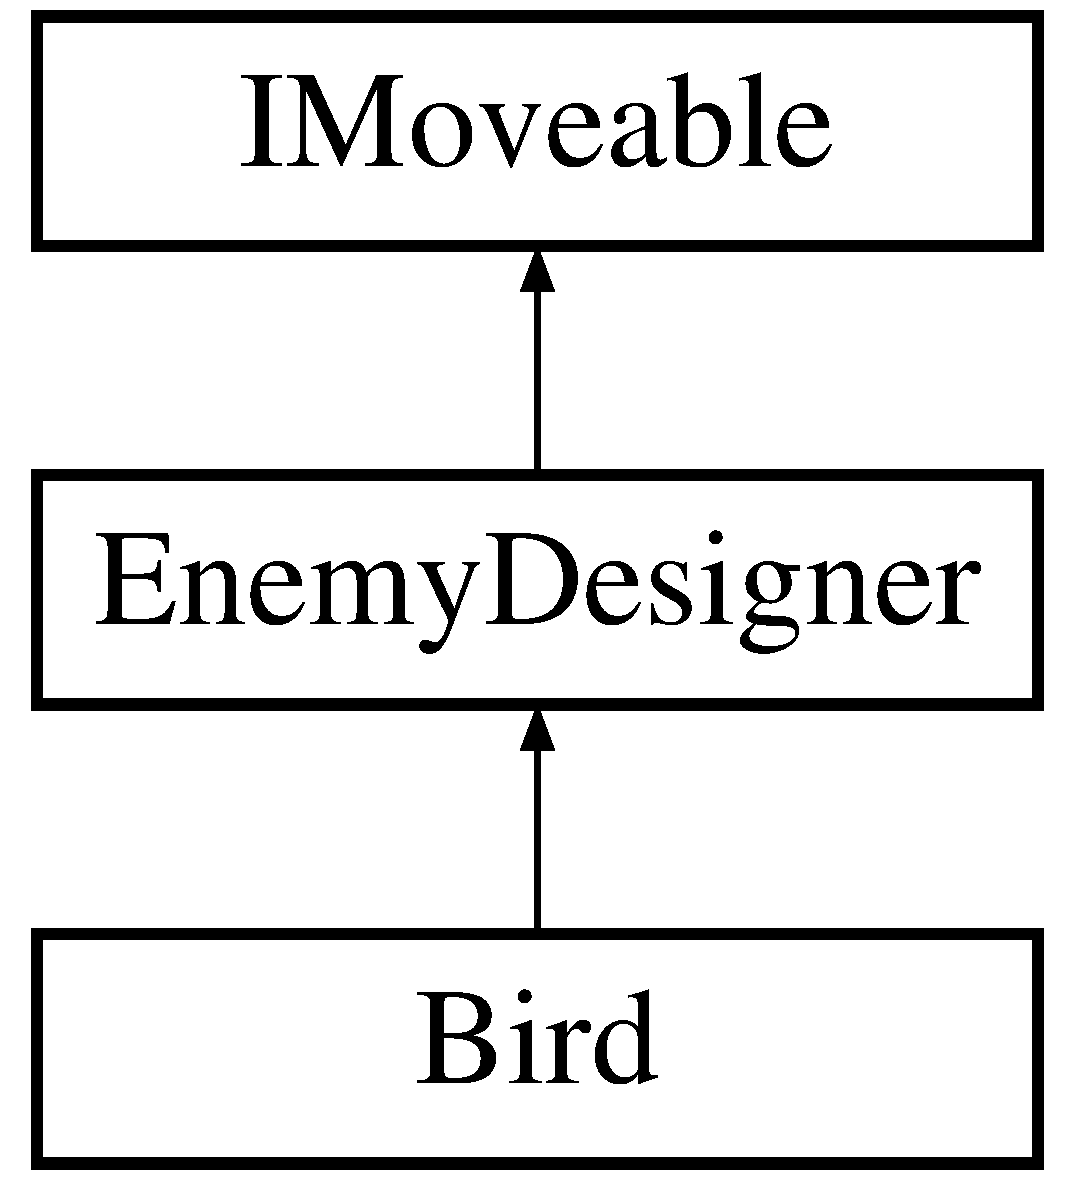
\includegraphics[height=3.000000cm]{class_bird}
\end{center}
\end{figure}
\subsection*{Public Member Functions}
\begin{DoxyCompactItemize}
\item 
\mbox{\hyperlink{class_bird_a8ada8cfd5d414ab4730651c37f86e348}{Bird}} (sf\+::\+Vector2f origin, sf\+::\+Vector2f dimensions, sf\+::\+Color color, sf\+::\+Vector2f texture\+Dimensions, std\+::string texture\+File=\char`\"{}set\+Of\+Monsters.\+png\char`\"{})
\begin{DoxyCompactList}\small\item\em constructor for bird class \end{DoxyCompactList}\end{DoxyCompactItemize}
\subsection*{Additional Inherited Members}


\subsection{Detailed Description}
Class representing bird. 

\subsection{Constructor \& Destructor Documentation}
\mbox{\Hypertarget{class_bird_a8ada8cfd5d414ab4730651c37f86e348}\label{class_bird_a8ada8cfd5d414ab4730651c37f86e348}} 
\index{Bird@{Bird}!Bird@{Bird}}
\index{Bird@{Bird}!Bird@{Bird}}
\subsubsection{\texorpdfstring{Bird()}{Bird()}}
{\footnotesize\ttfamily Bird\+::\+Bird (\begin{DoxyParamCaption}\item[{sf\+::\+Vector2f}]{origin,  }\item[{sf\+::\+Vector2f}]{dimensions,  }\item[{sf\+::\+Color}]{color,  }\item[{sf\+::\+Vector2f}]{texture\+Dimensions,  }\item[{std\+::string}]{texture\+File = {\ttfamily \char`\"{}setOfMonsters.png\char`\"{}} }\end{DoxyParamCaption})}



constructor for bird class 


\begin{DoxyParams}{Parameters}
{\em origin} & point \\
\hline
{\em dimensions} & \\
\hline
{\em color} & \\
\hline
{\em texture} & dimensions \\
\hline
{\em file} & containing texture \\
\hline
\end{DoxyParams}


The documentation for this class was generated from the following files\+:\begin{DoxyCompactItemize}
\item 
Tower\+Defence/\+Graphics\+Handler/Enemy\+Designer.\+h\item 
Tower\+Defence/\+Graphics\+Handler/Enemy\+Designer.\+cpp\end{DoxyCompactItemize}

\hypertarget{class_bullet_designer}{}\section{Bullet\+Designer Class Reference}
\label{class_bullet_designer}\index{Bullet\+Designer@{Bullet\+Designer}}


Class representing bullet.  




{\ttfamily \#include $<$Bullet\+Designer.\+h$>$}

Inheritance diagram for Bullet\+Designer\+:\begin{figure}[H]
\begin{center}
\leavevmode
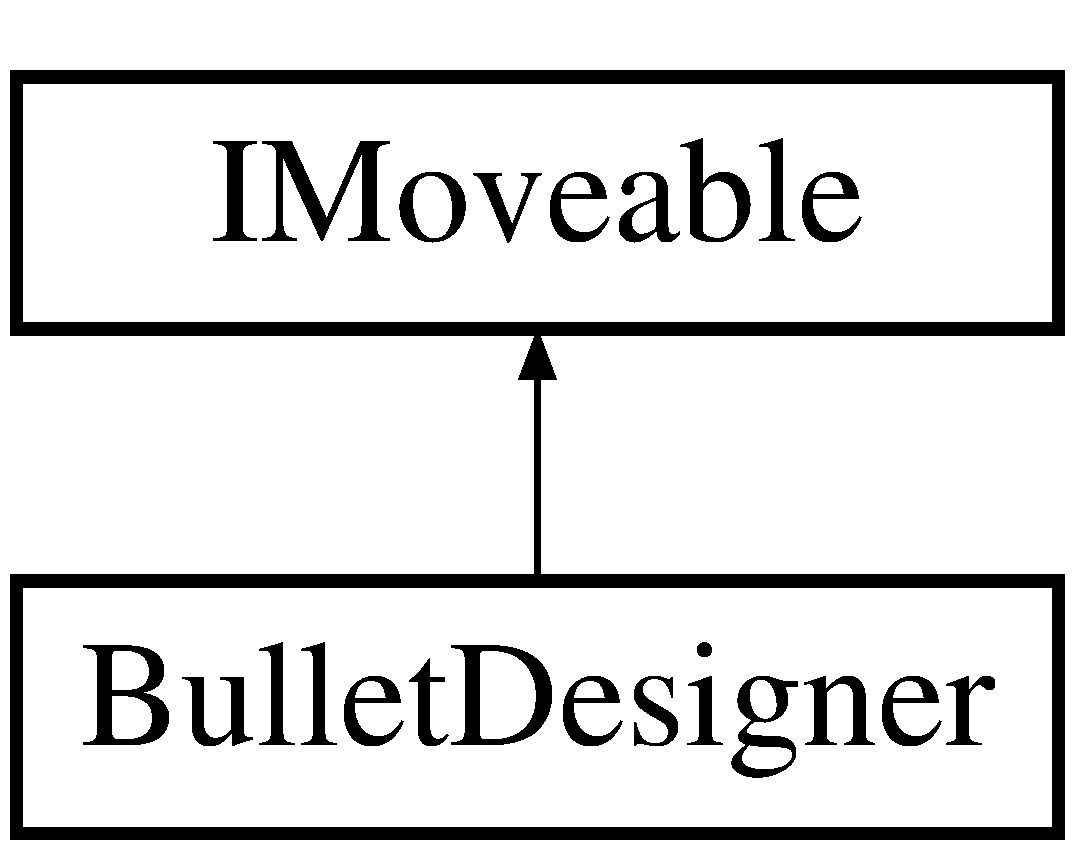
\includegraphics[height=2.000000cm]{class_bullet_designer}
\end{center}
\end{figure}
\subsection*{Public Member Functions}
\begin{DoxyCompactItemize}
\item 
\mbox{\hyperlink{class_bullet_designer_a4712950e2c64aaea2fe446855e8ec2d2}{Bullet\+Designer}} (sf\+::\+Vector2f start\+Point, sf\+::\+Vector2f destination\+Point, sf\+::\+Vector2f dimensions, uint damage, uint speed)
\begin{DoxyCompactList}\small\item\em constructor \end{DoxyCompactList}\item 
virtual uint \mbox{\hyperlink{class_bullet_designer_ab780d9e61cd46d6e2d1f73ad5144cb42}{Get\+Speed}} () override
\begin{DoxyCompactList}\small\item\em getter for bullet\textquotesingle{}s speed \end{DoxyCompactList}\item 
virtual void \mbox{\hyperlink{class_bullet_designer_a94ddb07bc126b159abc4cfedf27e18b7}{Move}} (const \mbox{\hyperlink{class_map}{Map}} \&m, const \mbox{\hyperlink{class_scene}{Scene}} \&scene) override
\begin{DoxyCompactList}\small\item\em Method for moving bullet on the map. \end{DoxyCompactList}\item 
virtual void \mbox{\hyperlink{class_bullet_designer_a5f920adb548d1e7d5e99394bebc08ec1}{draw}} (sf\+::\+Render\+Target \&target, sf\+::\+Render\+States states) override
\begin{DoxyCompactList}\small\item\em Method for drawing bullet (basing on current vertex array) \end{DoxyCompactList}\item 
virtual bool \mbox{\hyperlink{class_bullet_designer_a3ce40c948e1adcb694a1be0c10de0380}{Collides}} (\mbox{\hyperlink{class_i_moveable}{I\+Moveable}} $\ast$other) override
\begin{DoxyCompactList}\small\item\em Method for detecting collision with another object. \end{DoxyCompactList}\item 
virtual void \mbox{\hyperlink{class_bullet_designer_a360def48f566d8c863b1355b1cb69bad}{Collision}} (\mbox{\hyperlink{class_i_moveable}{I\+Moveable}} $\ast$other) override
\begin{DoxyCompactList}\small\item\em Method for performing collision with another object. \end{DoxyCompactList}\item 
virtual sf\+::\+Float\+Rect \mbox{\hyperlink{class_bullet_designer_ae7be5a8d1bef2c771715b5b8efce24ce}{Get\+Rect}} () override
\begin{DoxyCompactList}\small\item\em getter for bullet\textquotesingle{}s vertex array bounds \end{DoxyCompactList}\item 
virtual bool \mbox{\hyperlink{class_bullet_designer_a6287b58f72235fa91e103fa4400bdf12}{Removeable}} () override
\begin{DoxyCompactList}\small\item\em ~\newline
~\newline
Method returning m\+\_\+\+Move\+End value \end{DoxyCompactList}\item 
virtual sf\+::\+Vector2f \mbox{\hyperlink{class_bullet_designer_a89c3e817069b20e9404a01c3bdeaa481}{Get\+Origin}} () override
\begin{DoxyCompactList}\small\item\em getter for bullet\textquotesingle{}s origin point \end{DoxyCompactList}\item 
\mbox{\Hypertarget{class_bullet_designer_a0155587e64e09a997c2782e185b152f8}\label{class_bullet_designer_a0155587e64e09a997c2782e185b152f8}} 
\mbox{\hyperlink{class_bullet_designer_a0155587e64e09a997c2782e185b152f8}{$\sim$\+Bullet\+Designer}} ()
\begin{DoxyCompactList}\small\item\em destructor \end{DoxyCompactList}\end{DoxyCompactItemize}


\subsection{Detailed Description}
Class representing bullet. 

\subsection{Constructor \& Destructor Documentation}
\mbox{\Hypertarget{class_bullet_designer_a4712950e2c64aaea2fe446855e8ec2d2}\label{class_bullet_designer_a4712950e2c64aaea2fe446855e8ec2d2}} 
\index{Bullet\+Designer@{Bullet\+Designer}!Bullet\+Designer@{Bullet\+Designer}}
\index{Bullet\+Designer@{Bullet\+Designer}!Bullet\+Designer@{Bullet\+Designer}}
\subsubsection{\texorpdfstring{Bullet\+Designer()}{BulletDesigner()}}
{\footnotesize\ttfamily Bullet\+Designer\+::\+Bullet\+Designer (\begin{DoxyParamCaption}\item[{sf\+::\+Vector2f}]{start\+Point,  }\item[{sf\+::\+Vector2f}]{destination\+Point,  }\item[{sf\+::\+Vector2f}]{dimensions,  }\item[{uint}]{damage,  }\item[{uint}]{speed }\end{DoxyParamCaption})\hspace{0.3cm}{\ttfamily [explicit]}}



constructor 


\begin{DoxyParams}{Parameters}
{\em point} & from which bullet start \\
\hline
{\em destinating} & point where bullet hits \\
\hline
{\em dimensions} & of background rectangle \\
\hline
{\em bullet\textquotesingle{}s} & damage \\
\hline
{\em bullet\textquotesingle{}s} & speed \\
\hline
\end{DoxyParams}


\subsection{Member Function Documentation}
\mbox{\Hypertarget{class_bullet_designer_a3ce40c948e1adcb694a1be0c10de0380}\label{class_bullet_designer_a3ce40c948e1adcb694a1be0c10de0380}} 
\index{Bullet\+Designer@{Bullet\+Designer}!Collides@{Collides}}
\index{Collides@{Collides}!Bullet\+Designer@{Bullet\+Designer}}
\subsubsection{\texorpdfstring{Collides()}{Collides()}}
{\footnotesize\ttfamily bool Bullet\+Designer\+::\+Collides (\begin{DoxyParamCaption}\item[{\mbox{\hyperlink{class_i_moveable}{I\+Moveable}} $\ast$}]{other }\end{DoxyParamCaption})\hspace{0.3cm}{\ttfamily [override]}, {\ttfamily [virtual]}}



Method for detecting collision with another object. 


\begin{DoxyParams}{Parameters}
{\em reference} & to \mbox{\hyperlink{class_i_moveable}{I\+Moveable}} class,representing other object \\
\hline
\end{DoxyParams}
\begin{DoxyReturn}{Returns}
logical indicating whether collision happend 
\end{DoxyReturn}


Implements \mbox{\hyperlink{class_i_moveable}{I\+Moveable}}.

\mbox{\Hypertarget{class_bullet_designer_a360def48f566d8c863b1355b1cb69bad}\label{class_bullet_designer_a360def48f566d8c863b1355b1cb69bad}} 
\index{Bullet\+Designer@{Bullet\+Designer}!Collision@{Collision}}
\index{Collision@{Collision}!Bullet\+Designer@{Bullet\+Designer}}
\subsubsection{\texorpdfstring{Collision()}{Collision()}}
{\footnotesize\ttfamily void Bullet\+Designer\+::\+Collision (\begin{DoxyParamCaption}\item[{\mbox{\hyperlink{class_i_moveable}{I\+Moveable}} $\ast$}]{other }\end{DoxyParamCaption})\hspace{0.3cm}{\ttfamily [override]}, {\ttfamily [virtual]}}



Method for performing collision with another object. 


\begin{DoxyParams}{Parameters}
{\em reference} & to \mbox{\hyperlink{class_i_moveable}{I\+Moveable}} class,representing other object \\
\hline
\end{DoxyParams}


Implements \mbox{\hyperlink{class_i_moveable}{I\+Moveable}}.

\mbox{\Hypertarget{class_bullet_designer_a5f920adb548d1e7d5e99394bebc08ec1}\label{class_bullet_designer_a5f920adb548d1e7d5e99394bebc08ec1}} 
\index{Bullet\+Designer@{Bullet\+Designer}!draw@{draw}}
\index{draw@{draw}!Bullet\+Designer@{Bullet\+Designer}}
\subsubsection{\texorpdfstring{draw()}{draw()}}
{\footnotesize\ttfamily void Bullet\+Designer\+::draw (\begin{DoxyParamCaption}\item[{sf\+::\+Render\+Target \&}]{target,  }\item[{sf\+::\+Render\+States}]{states }\end{DoxyParamCaption})\hspace{0.3cm}{\ttfamily [override]}, {\ttfamily [virtual]}}



Method for drawing bullet (basing on current vertex array) 


\begin{DoxyParams}{Parameters}
{\em reference} & to Render\+Target class \\
\hline
{\em reference} & to Render\+States class \\
\hline
\end{DoxyParams}


Implements \mbox{\hyperlink{class_i_moveable}{I\+Moveable}}.

\mbox{\Hypertarget{class_bullet_designer_a89c3e817069b20e9404a01c3bdeaa481}\label{class_bullet_designer_a89c3e817069b20e9404a01c3bdeaa481}} 
\index{Bullet\+Designer@{Bullet\+Designer}!Get\+Origin@{Get\+Origin}}
\index{Get\+Origin@{Get\+Origin}!Bullet\+Designer@{Bullet\+Designer}}
\subsubsection{\texorpdfstring{Get\+Origin()}{GetOrigin()}}
{\footnotesize\ttfamily sf\+::\+Vector2f Bullet\+Designer\+::\+Get\+Origin (\begin{DoxyParamCaption}{ }\end{DoxyParamCaption})\hspace{0.3cm}{\ttfamily [override]}, {\ttfamily [virtual]}}



getter for bullet\textquotesingle{}s origin point 

\begin{DoxyReturn}{Returns}
origin point 
\end{DoxyReturn}


Implements \mbox{\hyperlink{class_i_moveable}{I\+Moveable}}.

\mbox{\Hypertarget{class_bullet_designer_ae7be5a8d1bef2c771715b5b8efce24ce}\label{class_bullet_designer_ae7be5a8d1bef2c771715b5b8efce24ce}} 
\index{Bullet\+Designer@{Bullet\+Designer}!Get\+Rect@{Get\+Rect}}
\index{Get\+Rect@{Get\+Rect}!Bullet\+Designer@{Bullet\+Designer}}
\subsubsection{\texorpdfstring{Get\+Rect()}{GetRect()}}
{\footnotesize\ttfamily sf\+::\+Float\+Rect Bullet\+Designer\+::\+Get\+Rect (\begin{DoxyParamCaption}{ }\end{DoxyParamCaption})\hspace{0.3cm}{\ttfamily [override]}, {\ttfamily [virtual]}}



getter for bullet\textquotesingle{}s vertex array bounds 

\begin{DoxyReturn}{Returns}
vertex array boundaries 
\end{DoxyReturn}


Implements \mbox{\hyperlink{class_i_moveable}{I\+Moveable}}.

\mbox{\Hypertarget{class_bullet_designer_ab780d9e61cd46d6e2d1f73ad5144cb42}\label{class_bullet_designer_ab780d9e61cd46d6e2d1f73ad5144cb42}} 
\index{Bullet\+Designer@{Bullet\+Designer}!Get\+Speed@{Get\+Speed}}
\index{Get\+Speed@{Get\+Speed}!Bullet\+Designer@{Bullet\+Designer}}
\subsubsection{\texorpdfstring{Get\+Speed()}{GetSpeed()}}
{\footnotesize\ttfamily uint Bullet\+Designer\+::\+Get\+Speed (\begin{DoxyParamCaption}{ }\end{DoxyParamCaption})\hspace{0.3cm}{\ttfamily [override]}, {\ttfamily [virtual]}}



getter for bullet\textquotesingle{}s speed 

\begin{DoxyReturn}{Returns}
bullet\textquotesingle{}s speed 
\end{DoxyReturn}


Implements \mbox{\hyperlink{class_i_moveable}{I\+Moveable}}.

\mbox{\Hypertarget{class_bullet_designer_a94ddb07bc126b159abc4cfedf27e18b7}\label{class_bullet_designer_a94ddb07bc126b159abc4cfedf27e18b7}} 
\index{Bullet\+Designer@{Bullet\+Designer}!Move@{Move}}
\index{Move@{Move}!Bullet\+Designer@{Bullet\+Designer}}
\subsubsection{\texorpdfstring{Move()}{Move()}}
{\footnotesize\ttfamily void Bullet\+Designer\+::\+Move (\begin{DoxyParamCaption}\item[{const \mbox{\hyperlink{class_map}{Map}} \&}]{m,  }\item[{const \mbox{\hyperlink{class_scene}{Scene}} \&}]{scene }\end{DoxyParamCaption})\hspace{0.3cm}{\ttfamily [override]}, {\ttfamily [virtual]}}



Method for moving bullet on the map. 


\begin{DoxyParams}{Parameters}
{\em reference} & to \mbox{\hyperlink{class_map}{Map}} class \\
\hline
{\em reference} & to \mbox{\hyperlink{class_scene}{Scene}} class \\
\hline
\end{DoxyParams}


Implements \mbox{\hyperlink{class_i_moveable}{I\+Moveable}}.

\mbox{\Hypertarget{class_bullet_designer_a6287b58f72235fa91e103fa4400bdf12}\label{class_bullet_designer_a6287b58f72235fa91e103fa4400bdf12}} 
\index{Bullet\+Designer@{Bullet\+Designer}!Removeable@{Removeable}}
\index{Removeable@{Removeable}!Bullet\+Designer@{Bullet\+Designer}}
\subsubsection{\texorpdfstring{Removeable()}{Removeable()}}
{\footnotesize\ttfamily bool Bullet\+Designer\+::\+Removeable (\begin{DoxyParamCaption}{ }\end{DoxyParamCaption})\hspace{0.3cm}{\ttfamily [override]}, {\ttfamily [virtual]}}



~\newline
~\newline
Method returning m\+\_\+\+Move\+End value 

\begin{DoxyReturn}{Returns}
boolean indicating whether end was reached 
\end{DoxyReturn}


Implements \mbox{\hyperlink{class_i_moveable}{I\+Moveable}}.



The documentation for this class was generated from the following files\+:\begin{DoxyCompactItemize}
\item 
Tower\+Defence/\+Graphics\+Handler/Bullet\+Designer.\+h\item 
Tower\+Defence/\+Graphics\+Handler/Bullet\+Designer.\+cpp\end{DoxyCompactItemize}

\hypertarget{class_configuration_manager}{}\section{Configuration\+Manager Class Reference}
\label{class_configuration_manager}\index{Configuration\+Manager@{Configuration\+Manager}}


Class responsible for reading game\textquotesingle{}s properties from xml file.  




{\ttfamily \#include $<$Configuration\+Manager.\+h$>$}

\subsection*{Public Member Functions}
\begin{DoxyCompactItemize}
\item 
\mbox{\hyperlink{class_configuration_manager_aee85c207758968e5ce0c291383aa51f6}{Configuration\+Manager}} (std\+::string \mbox{\hyperlink{classrapidxml_1_1file}{file}}=\char`\"{}config.\+xml\char`\"{})
\begin{DoxyCompactList}\small\item\em constructor \end{DoxyCompactList}\item 
\mbox{\Hypertarget{class_configuration_manager_ae4a92204b4d685954df9249330adaca6}\label{class_configuration_manager_ae4a92204b4d685954df9249330adaca6}} 
void \mbox{\hyperlink{class_configuration_manager_ae4a92204b4d685954df9249330adaca6}{read\+Configuration}} ()
\begin{DoxyCompactList}\small\item\em configuration reader Method reads configuration from specified file. It uses rapidxml library \end{DoxyCompactList}\item 
\mbox{\Hypertarget{class_configuration_manager_ab0484bee60058310602a8148bc668200}\label{class_configuration_manager_ab0484bee60058310602a8148bc668200}} 
std\+::vector$<$ \mbox{\hyperlink{class_level}{Level}} $>$ \mbox{\hyperlink{class_configuration_manager_ab0484bee60058310602a8148bc668200}{get\+Levels}} ()
\begin{DoxyCompactList}\small\item\em getter for vector of levels \end{DoxyCompactList}\end{DoxyCompactItemize}
\subsection*{Public Attributes}
\begin{DoxyCompactItemize}
\item 
\mbox{\Hypertarget{class_configuration_manager_a055385b86b26a736af6ba2d24477a5b2}\label{class_configuration_manager_a055385b86b26a736af6ba2d24477a5b2}} 
int {\bfseries number\+Of\+Levels}
\end{DoxyCompactItemize}


\subsection{Detailed Description}
Class responsible for reading game\textquotesingle{}s properties from xml file. 

\subsection{Constructor \& Destructor Documentation}
\mbox{\Hypertarget{class_configuration_manager_aee85c207758968e5ce0c291383aa51f6}\label{class_configuration_manager_aee85c207758968e5ce0c291383aa51f6}} 
\index{Configuration\+Manager@{Configuration\+Manager}!Configuration\+Manager@{Configuration\+Manager}}
\index{Configuration\+Manager@{Configuration\+Manager}!Configuration\+Manager@{Configuration\+Manager}}
\subsubsection{\texorpdfstring{Configuration\+Manager()}{ConfigurationManager()}}
{\footnotesize\ttfamily Configuration\+Manager\+::\+Configuration\+Manager (\begin{DoxyParamCaption}\item[{std\+::string}]{config\+File = {\ttfamily \char`\"{}config.xml\char`\"{}} }\end{DoxyParamCaption})}



constructor 


\begin{DoxyParams}{Parameters}
{\em config} & file name \\
\hline
\end{DoxyParams}


The documentation for this class was generated from the following files\+:\begin{DoxyCompactItemize}
\item 
Tower\+Defence/\+Graphics\+Handler/Configuration\+Manager.\+h\item 
Tower\+Defence/\+Graphics\+Handler/Configuration\+Manager.\+cpp\end{DoxyCompactItemize}

\hypertarget{class_custom_exception}{}\section{Custom\+Exception Class Reference}
\label{class_custom_exception}\index{Custom\+Exception@{Custom\+Exception}}


Class used for providing custom exceptions.  




{\ttfamily \#include $<$Utils.\+hpp$>$}

Inheritance diagram for Custom\+Exception\+:\begin{figure}[H]
\begin{center}
\leavevmode
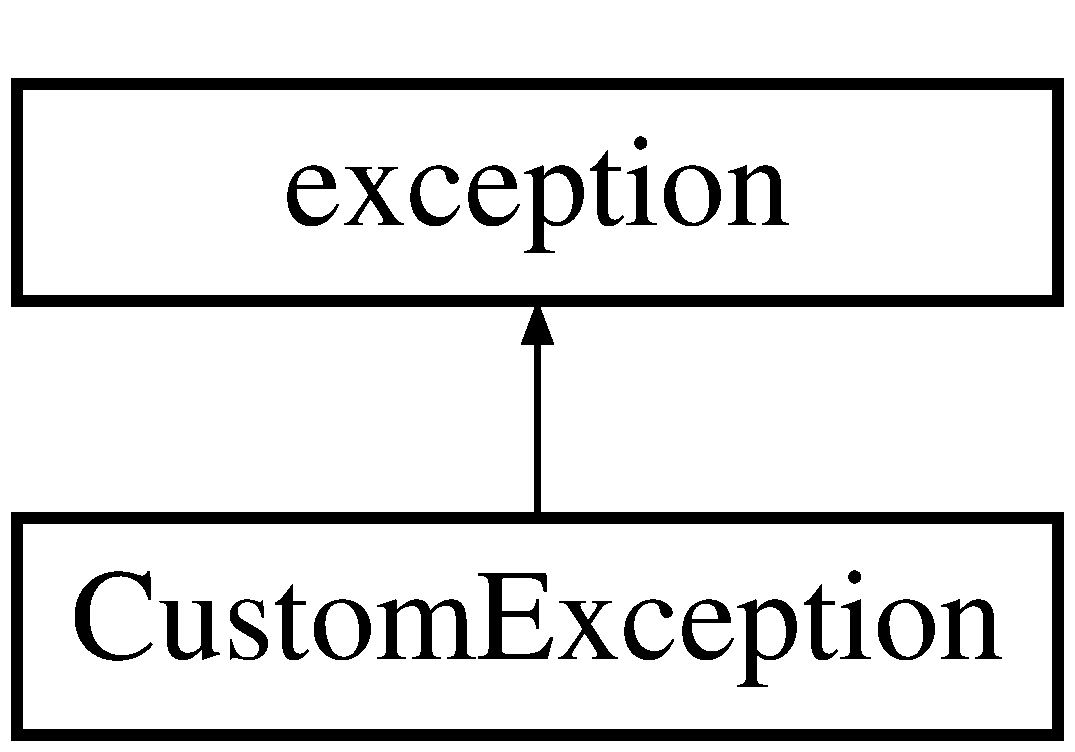
\includegraphics[height=2.000000cm]{class_custom_exception}
\end{center}
\end{figure}
\subsection*{Public Member Functions}
\begin{DoxyCompactItemize}
\item 
\mbox{\Hypertarget{class_custom_exception_a2e4226b49820b0cc7408ad5fa62b061a}\label{class_custom_exception_a2e4226b49820b0cc7408ad5fa62b061a}} 
{\bfseries Custom\+Exception} (std\+::string message)
\item 
\mbox{\Hypertarget{class_custom_exception_a2b382e4dd37ef2af58162fdf2087318d}\label{class_custom_exception_a2b382e4dd37ef2af58162fdf2087318d}} 
virtual const char $\ast$ {\bfseries what} () const  throw ()
\end{DoxyCompactItemize}


\subsection{Detailed Description}
Class used for providing custom exceptions. 

The documentation for this class was generated from the following file\+:\begin{DoxyCompactItemize}
\item 
Tower\+Defence/\+Graphics\+Handler/Utils.\+hpp\end{DoxyCompactItemize}

\hypertarget{class_enemy_base}{}\section{Enemy\+Base Class Reference}
\label{class_enemy_base}\index{Enemy\+Base@{Enemy\+Base}}


Class representing logical part of enemy.  




{\ttfamily \#include $<$Enemy\+Base.\+hpp$>$}

\subsection*{Public Member Functions}
\begin{DoxyCompactItemize}
\item 
\mbox{\hyperlink{class_point}{Point}} \mbox{\hyperlink{class_enemy_base_a95652c26aa4a75f69b7dac1c63ccde95}{get\+Position}} ()
\begin{DoxyCompactList}\small\item\em getter for Enemy\textquotesingle{}s position \end{DoxyCompactList}\item 
void \mbox{\hyperlink{class_enemy_base_aeae4a4336e40f2f799fafaef9e21f61b}{Step}} (const \mbox{\hyperlink{class_map}{Map}} \&m)
\begin{DoxyCompactList}\small\item\em Methods for making step on the map It takes next position of the point and set current position to that point. \end{DoxyCompactList}\item 
\mbox{\Hypertarget{class_enemy_base_a24272609863449e7e0502af45450c089}\label{class_enemy_base_a24272609863449e7e0502af45450c089}} 
void \mbox{\hyperlink{class_enemy_base_a24272609863449e7e0502af45450c089}{set\+Health}} (int health)
\begin{DoxyCompactList}\small\item\em ~\newline
setter for Enemy\textquotesingle{}s health \end{DoxyCompactList}\item 
int \mbox{\hyperlink{class_enemy_base_accad87636833f0ce585eb1294122d3b3}{Get\+Health}} ()
\begin{DoxyCompactList}\small\item\em getter for Enemy\textquotesingle{}s health \end{DoxyCompactList}\item 
int \mbox{\hyperlink{class_enemy_base_a4ab9a0cedd83a58215f37eb9e3eb9469}{Get\+Speed}} ()
\begin{DoxyCompactList}\small\item\em getter for speed \end{DoxyCompactList}\item 
int \mbox{\hyperlink{class_enemy_base_a7187da0f23cc619b9ebca37d9adb9b96}{Get\+Value}} ()
\begin{DoxyCompactList}\small\item\em getter for stats value \end{DoxyCompactList}\item 
int \mbox{\hyperlink{class_enemy_base_a6d4acbc673477c11d376bfd695e38b77}{Get\+Damage}} ()
\begin{DoxyCompactList}\small\item\em getter for damage \end{DoxyCompactList}\item 
\mbox{\Hypertarget{class_enemy_base_af0e688056ae50b763bb8d8139e7e53c3}\label{class_enemy_base_af0e688056ae50b763bb8d8139e7e53c3}} 
\mbox{\hyperlink{class_enemy_base_af0e688056ae50b763bb8d8139e7e53c3}{Enemy\+Base}} ()
\begin{DoxyCompactList}\small\item\em constructor \end{DoxyCompactList}\item 
\mbox{\hyperlink{class_enemy_base_a3a5fda450d95f680a394c171669a6266}{Enemy\+Base}} (\mbox{\hyperlink{class_point}{Point}} p)
\begin{DoxyCompactList}\small\item\em constructor with parameter this constructor takes point as parameter and set current position to this point \end{DoxyCompactList}\item 
\mbox{\hyperlink{class_enemy_base_a6ba829dd786e4409282b022195dadea5}{Enemy\+Base}} (uint health, uint damage, uint speed)
\begin{DoxyCompactList}\small\item\em constructor with parameters this constructor takes health,damage and speed as parameters and set statistics to those values \end{DoxyCompactList}\item 
\mbox{\hyperlink{class_enemy_base_ac4982e903a34b0a98f3ada74ef7a416f}{Enemy\+Base}} (\mbox{\hyperlink{class_point}{Point}} p, uint health, uint damage, uint speed)
\begin{DoxyCompactList}\small\item\em constructor with parameters this constructor takes point, health, damage and speed as parameters and set those values \end{DoxyCompactList}\item 
\mbox{\Hypertarget{class_enemy_base_a73d1ffb3230a2e8b2c0b7cd86cbd7a6c}\label{class_enemy_base_a73d1ffb3230a2e8b2c0b7cd86cbd7a6c}} 
\mbox{\hyperlink{class_enemy_base_a73d1ffb3230a2e8b2c0b7cd86cbd7a6c}{$\sim$\+Enemy\+Base}} ()
\begin{DoxyCompactList}\small\item\em destructor \end{DoxyCompactList}\end{DoxyCompactItemize}
\subsection*{Protected Attributes}
\begin{DoxyCompactItemize}
\item 
\mbox{\Hypertarget{class_enemy_base_af5e4b032a3bc2d9a4f3f82bb2bacfc98}\label{class_enemy_base_af5e4b032a3bc2d9a4f3f82bb2bacfc98}} 
\mbox{\hyperlink{class_point}{Point}} {\bfseries m\+\_\+\+Position}
\item 
\mbox{\Hypertarget{class_enemy_base_a2b4cce074350fa64dd888efa159526db}\label{class_enemy_base_a2b4cce074350fa64dd888efa159526db}} 
\mbox{\hyperlink{class_statistics}{Statistics}} {\bfseries m\+\_\+\+Stats}
\end{DoxyCompactItemize}


\subsection{Detailed Description}
Class representing logical part of enemy. 

\subsection{Constructor \& Destructor Documentation}
\mbox{\Hypertarget{class_enemy_base_a3a5fda450d95f680a394c171669a6266}\label{class_enemy_base_a3a5fda450d95f680a394c171669a6266}} 
\index{Enemy\+Base@{Enemy\+Base}!Enemy\+Base@{Enemy\+Base}}
\index{Enemy\+Base@{Enemy\+Base}!Enemy\+Base@{Enemy\+Base}}
\subsubsection{\texorpdfstring{Enemy\+Base()}{EnemyBase()}\hspace{0.1cm}{\footnotesize\ttfamily [1/3]}}
{\footnotesize\ttfamily Enemy\+Base\+::\+Enemy\+Base (\begin{DoxyParamCaption}\item[{\mbox{\hyperlink{class_point}{Point}}}]{p }\end{DoxyParamCaption})}



constructor with parameter this constructor takes point as parameter and set current position to this point 


\begin{DoxyParams}{Parameters}
{\em \mbox{\hyperlink{class_point}{Point}}} & \\
\hline
\end{DoxyParams}
\mbox{\Hypertarget{class_enemy_base_a6ba829dd786e4409282b022195dadea5}\label{class_enemy_base_a6ba829dd786e4409282b022195dadea5}} 
\index{Enemy\+Base@{Enemy\+Base}!Enemy\+Base@{Enemy\+Base}}
\index{Enemy\+Base@{Enemy\+Base}!Enemy\+Base@{Enemy\+Base}}
\subsubsection{\texorpdfstring{Enemy\+Base()}{EnemyBase()}\hspace{0.1cm}{\footnotesize\ttfamily [2/3]}}
{\footnotesize\ttfamily Enemy\+Base\+::\+Enemy\+Base (\begin{DoxyParamCaption}\item[{uint}]{health,  }\item[{uint}]{damage,  }\item[{uint}]{speed }\end{DoxyParamCaption})}



constructor with parameters this constructor takes health,damage and speed as parameters and set statistics to those values 


\begin{DoxyParams}{Parameters}
{\em health} & \\
\hline
{\em damage} & \\
\hline
{\em speed} & \\
\hline
\end{DoxyParams}
\mbox{\Hypertarget{class_enemy_base_ac4982e903a34b0a98f3ada74ef7a416f}\label{class_enemy_base_ac4982e903a34b0a98f3ada74ef7a416f}} 
\index{Enemy\+Base@{Enemy\+Base}!Enemy\+Base@{Enemy\+Base}}
\index{Enemy\+Base@{Enemy\+Base}!Enemy\+Base@{Enemy\+Base}}
\subsubsection{\texorpdfstring{Enemy\+Base()}{EnemyBase()}\hspace{0.1cm}{\footnotesize\ttfamily [3/3]}}
{\footnotesize\ttfamily Enemy\+Base\+::\+Enemy\+Base (\begin{DoxyParamCaption}\item[{\mbox{\hyperlink{class_point}{Point}}}]{p,  }\item[{uint}]{health,  }\item[{uint}]{damage,  }\item[{uint}]{speed }\end{DoxyParamCaption})}



constructor with parameters this constructor takes point, health, damage and speed as parameters and set those values 


\begin{DoxyParams}{Parameters}
{\em \mbox{\hyperlink{class_point}{Point}}} & \\
\hline
{\em health} & \\
\hline
{\em damage} & \\
\hline
{\em speed} & \\
\hline
\end{DoxyParams}


\subsection{Member Function Documentation}
\mbox{\Hypertarget{class_enemy_base_a6d4acbc673477c11d376bfd695e38b77}\label{class_enemy_base_a6d4acbc673477c11d376bfd695e38b77}} 
\index{Enemy\+Base@{Enemy\+Base}!Get\+Damage@{Get\+Damage}}
\index{Get\+Damage@{Get\+Damage}!Enemy\+Base@{Enemy\+Base}}
\subsubsection{\texorpdfstring{Get\+Damage()}{GetDamage()}}
{\footnotesize\ttfamily int Enemy\+Base\+::\+Get\+Damage (\begin{DoxyParamCaption}{ }\end{DoxyParamCaption})}



getter for damage 

\begin{DoxyReturn}{Returns}
damage 
\end{DoxyReturn}
\mbox{\Hypertarget{class_enemy_base_accad87636833f0ce585eb1294122d3b3}\label{class_enemy_base_accad87636833f0ce585eb1294122d3b3}} 
\index{Enemy\+Base@{Enemy\+Base}!Get\+Health@{Get\+Health}}
\index{Get\+Health@{Get\+Health}!Enemy\+Base@{Enemy\+Base}}
\subsubsection{\texorpdfstring{Get\+Health()}{GetHealth()}}
{\footnotesize\ttfamily int Enemy\+Base\+::\+Get\+Health (\begin{DoxyParamCaption}{ }\end{DoxyParamCaption})}



getter for Enemy\textquotesingle{}s health 

\begin{DoxyReturn}{Returns}
health 
\end{DoxyReturn}
\mbox{\Hypertarget{class_enemy_base_a95652c26aa4a75f69b7dac1c63ccde95}\label{class_enemy_base_a95652c26aa4a75f69b7dac1c63ccde95}} 
\index{Enemy\+Base@{Enemy\+Base}!get\+Position@{get\+Position}}
\index{get\+Position@{get\+Position}!Enemy\+Base@{Enemy\+Base}}
\subsubsection{\texorpdfstring{get\+Position()}{getPosition()}}
{\footnotesize\ttfamily \mbox{\hyperlink{class_point}{Point}} Enemy\+Base\+::get\+Position (\begin{DoxyParamCaption}{ }\end{DoxyParamCaption})}



getter for Enemy\textquotesingle{}s position 

\begin{DoxyReturn}{Returns}
enemy position 
\end{DoxyReturn}
\mbox{\Hypertarget{class_enemy_base_a4ab9a0cedd83a58215f37eb9e3eb9469}\label{class_enemy_base_a4ab9a0cedd83a58215f37eb9e3eb9469}} 
\index{Enemy\+Base@{Enemy\+Base}!Get\+Speed@{Get\+Speed}}
\index{Get\+Speed@{Get\+Speed}!Enemy\+Base@{Enemy\+Base}}
\subsubsection{\texorpdfstring{Get\+Speed()}{GetSpeed()}}
{\footnotesize\ttfamily int Enemy\+Base\+::\+Get\+Speed (\begin{DoxyParamCaption}{ }\end{DoxyParamCaption})}



getter for speed 

\begin{DoxyReturn}{Returns}
speed 
\end{DoxyReturn}
\mbox{\Hypertarget{class_enemy_base_a7187da0f23cc619b9ebca37d9adb9b96}\label{class_enemy_base_a7187da0f23cc619b9ebca37d9adb9b96}} 
\index{Enemy\+Base@{Enemy\+Base}!Get\+Value@{Get\+Value}}
\index{Get\+Value@{Get\+Value}!Enemy\+Base@{Enemy\+Base}}
\subsubsection{\texorpdfstring{Get\+Value()}{GetValue()}}
{\footnotesize\ttfamily int Enemy\+Base\+::\+Get\+Value (\begin{DoxyParamCaption}{ }\end{DoxyParamCaption})}



getter for stats value 

\begin{DoxyReturn}{Returns}
value 
\end{DoxyReturn}
\mbox{\Hypertarget{class_enemy_base_aeae4a4336e40f2f799fafaef9e21f61b}\label{class_enemy_base_aeae4a4336e40f2f799fafaef9e21f61b}} 
\index{Enemy\+Base@{Enemy\+Base}!Step@{Step}}
\index{Step@{Step}!Enemy\+Base@{Enemy\+Base}}
\subsubsection{\texorpdfstring{Step()}{Step()}}
{\footnotesize\ttfamily void Enemy\+Base\+::\+Step (\begin{DoxyParamCaption}\item[{const \mbox{\hyperlink{class_map}{Map}} \&}]{m }\end{DoxyParamCaption})}



Methods for making step on the map It takes next position of the point and set current position to that point. 


\begin{DoxyParams}{Parameters}
{\em reference} & to \mbox{\hyperlink{class_map}{Map}} \\
\hline
\end{DoxyParams}


The documentation for this class was generated from the following files\+:\begin{DoxyCompactItemize}
\item 
Tower\+Defence/\+Graphics\+Handler/Enemy\+Base.\+hpp\item 
Tower\+Defence/\+Graphics\+Handler/Enemy\+Base.\+cpp\end{DoxyCompactItemize}

\hypertarget{class_enemy_designer}{}\section{Enemy\+Designer Class Reference}
\label{class_enemy_designer}\index{Enemy\+Designer@{Enemy\+Designer}}


Class representing physical enemy.  




{\ttfamily \#include $<$Enemy\+Designer.\+h$>$}

Inheritance diagram for Enemy\+Designer\+:\begin{figure}[H]
\begin{center}
\leavevmode
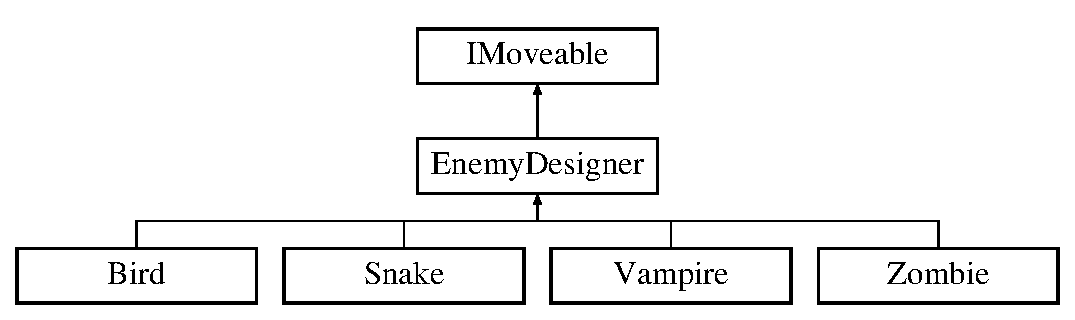
\includegraphics[height=3.000000cm]{class_enemy_designer}
\end{center}
\end{figure}
\subsection*{Public Member Functions}
\begin{DoxyCompactItemize}
\item 
\mbox{\hyperlink{class_enemy_designer_a976f7ec242432ef9d2eb7c181590833b}{Enemy\+Designer}} (\mbox{\hyperlink{class_enemy_base}{Enemy\+Base}} enemy\+Object, sf\+::\+Vector2f origin, sf\+::\+Vector2f dimensions, sf\+::\+Color color, sf\+::\+Vector2f texture\+Origin=sf\+::\+Vector2f(0, 0))
\begin{DoxyCompactList}\small\item\em constructor \end{DoxyCompactList}\item 
sf\+::\+Vertex\+Array \mbox{\hyperlink{class_enemy_designer_a699a16e808c173c28dc7be7c05386ea1}{get\+Enemy\+Vertex}} ()
\begin{DoxyCompactList}\small\item\em getter for enemy vertex \end{DoxyCompactList}\item 
\mbox{\Hypertarget{class_enemy_designer_a49fd1cb02ff43f7c3264f46ca9f94cb0}\label{class_enemy_designer_a49fd1cb02ff43f7c3264f46ca9f94cb0}} 
void {\bfseries Update\+Origin} (sf\+::\+Vector2f new\+Origin)
\item 
uint \mbox{\hyperlink{class_enemy_designer_a4a1fc18b37685368194461f744937d22}{Get\+Steps}} ()
\begin{DoxyCompactList}\small\item\em getter for steps \end{DoxyCompactList}\item 
virtual sf\+::\+Vector2f \mbox{\hyperlink{class_enemy_designer_a868f397544fe2415d1d6881e7b3acf92}{Get\+Origin}} () override
\begin{DoxyCompactList}\small\item\em getter for origin point \end{DoxyCompactList}\item 
virtual uint \mbox{\hyperlink{class_enemy_designer_a857e6d38180ed66dacb0ba8bfcd02173}{Get\+Speed}} () override
\begin{DoxyCompactList}\small\item\em getter for speed \end{DoxyCompactList}\item 
virtual void \mbox{\hyperlink{class_enemy_designer_a0aa9fb702dc95ad548108379ba3540a8}{Move}} (const \mbox{\hyperlink{class_map}{Map}} \&m, const \mbox{\hyperlink{class_scene}{Scene}} \&scene) override
\begin{DoxyCompactList}\small\item\em Method used for moving object on the map If object isn\textquotesingle{}t moving it gets the destination point from scene. \end{DoxyCompactList}\item 
virtual void \mbox{\hyperlink{class_enemy_designer_ab496f15186e05c356bbdb7931fed56b6}{draw}} (sf\+::\+Render\+Target \&target, sf\+::\+Render\+States states) override
\begin{DoxyCompactList}\small\item\em Method used for drawing object basing on vertex array and tileset. \end{DoxyCompactList}\item 
virtual bool \mbox{\hyperlink{class_enemy_designer_aaea93aae4a87f999f2f11233aca161c1}{Collides}} (\mbox{\hyperlink{class_i_moveable}{I\+Moveable}} $\ast$other) override
\item 
virtual void \mbox{\hyperlink{class_enemy_designer_a2d9fb6cc11f8f975b263d6739a1a3ac2}{Collision}} (\mbox{\hyperlink{class_i_moveable}{I\+Moveable}} $\ast$other) override
\begin{DoxyCompactList}\small\item\em Method used for collision detection method sets collision delay according to defined C\+O\+L\+L\+I\+S\+I\+O\+N\+\_\+\+D\+E\+L\+A\+Y\+\_\+\+V\+A\+L\+UE. \end{DoxyCompactList}\item 
virtual sf\+::\+Float\+Rect \mbox{\hyperlink{class_enemy_designer_a1dc87f5766601115601c20de865ef6d7}{Get\+Rect}} () override
\begin{DoxyCompactList}\small\item\em Getter for vertex points. \end{DoxyCompactList}\item 
virtual bool \mbox{\hyperlink{class_enemy_designer_a721c45f9d14c10f55b2d7ae624e2db6a}{Removeable}} () override
\begin{DoxyCompactList}\small\item\em Method checks whether health is lower than 0 so it can be removed. \end{DoxyCompactList}\item 
void \mbox{\hyperlink{class_enemy_designer_a6aac3b8c8fa145212a1d37a1f1bcaca7}{Hit}} (uint amount)
\begin{DoxyCompactList}\small\item\em Method used for changing health when being hit. \end{DoxyCompactList}\item 
\mbox{\hyperlink{class_point}{Point}} \mbox{\hyperlink{class_enemy_designer_a3ed8aa13f9da30df073e729ea4817dfe}{Get\+Position}} ()
\begin{DoxyCompactList}\small\item\em getter for position \end{DoxyCompactList}\item 
int \mbox{\hyperlink{class_enemy_designer_aa1982407303eb55be476281c5b7a40f8}{Get\+Value}} ()
\begin{DoxyCompactList}\small\item\em getter for value of the enemy \end{DoxyCompactList}\item 
int \mbox{\hyperlink{class_enemy_designer_a6c612e70cef0534946c54f302f63a970}{Get\+Damage}} ()
\begin{DoxyCompactList}\small\item\em getter for enemy\textquotesingle{}s damage \end{DoxyCompactList}\item 
virtual void \mbox{\hyperlink{class_enemy_designer_afaed42dca9d945456c780c55a6c16b84}{set\+Health}} (uint health)
\begin{DoxyCompactList}\small\item\em Setter for enemy\textquotesingle{}s health. \end{DoxyCompactList}\item 
\mbox{\Hypertarget{class_enemy_designer_ac7938c26b4e2f54b511c1e18cdacb97b}\label{class_enemy_designer_ac7938c26b4e2f54b511c1e18cdacb97b}} 
\mbox{\hyperlink{class_enemy_designer_ac7938c26b4e2f54b511c1e18cdacb97b}{$\sim$\+Enemy\+Designer}} ()
\begin{DoxyCompactList}\small\item\em destructor \end{DoxyCompactList}\end{DoxyCompactItemize}
\subsection*{Public Attributes}
\begin{DoxyCompactItemize}
\item 
\mbox{\Hypertarget{class_enemy_designer_af003889b786feb80d2330115959a2530}\label{class_enemy_designer_af003889b786feb80d2330115959a2530}} 
std\+::string {\bfseries transparency\+Color}
\end{DoxyCompactItemize}
\subsection*{Protected Member Functions}
\begin{DoxyCompactItemize}
\item 
\mbox{\Hypertarget{class_enemy_designer_ac9518d4725dc0c6bfe65dcdefa72f67e}\label{class_enemy_designer_ac9518d4725dc0c6bfe65dcdefa72f67e}} 
void \mbox{\hyperlink{class_enemy_designer_ac9518d4725dc0c6bfe65dcdefa72f67e}{step}} ()
\begin{DoxyCompactList}\small\item\em Method used for performing step of enemy it tests whether enemy hits something in x and y axis. \end{DoxyCompactList}\item 
\mbox{\Hypertarget{class_enemy_designer_a7148adb40736b887e9b9bd5cd5587e7a}\label{class_enemy_designer_a7148adb40736b887e9b9bd5cd5587e7a}} 
void \mbox{\hyperlink{class_enemy_designer_a7148adb40736b887e9b9bd5cd5587e7a}{Move\+To\+Point}} ()
\begin{DoxyCompactList}\small\item\em Method used for moving towards point it performs move when distance in x and y directions are greater than 0. \end{DoxyCompactList}\item 
\mbox{\Hypertarget{class_enemy_designer_a856d62edac7271e1c9031eae3e9e156c}\label{class_enemy_designer_a856d62edac7271e1c9031eae3e9e156c}} 
void \mbox{\hyperlink{class_enemy_designer_a856d62edac7271e1c9031eae3e9e156c}{Update\+Vertex}} ()
\begin{DoxyCompactList}\small\item\em Method used for updating vertex method calculates rectangle\textquotesingle{}s corners basing on current origin and dimensions. \end{DoxyCompactList}\end{DoxyCompactItemize}
\subsection*{Protected Attributes}
\begin{DoxyCompactItemize}
\item 
\mbox{\Hypertarget{class_enemy_designer_a4bd433eb71119492c95204c72d9f7a35}\label{class_enemy_designer_a4bd433eb71119492c95204c72d9f7a35}} 
sf\+::\+Vector2f {\bfseries m\+\_\+dimensions}
\item 
\mbox{\Hypertarget{class_enemy_designer_ac9cad159fc1f9fb7caf997a72b682d8a}\label{class_enemy_designer_ac9cad159fc1f9fb7caf997a72b682d8a}} 
sf\+::\+Color {\bfseries m\+\_\+color}
\item 
\mbox{\Hypertarget{class_enemy_designer_aa1317c9f36bc81eba0bba16097a61728}\label{class_enemy_designer_aa1317c9f36bc81eba0bba16097a61728}} 
sf\+::\+Vertex\+Array {\bfseries m\+\_\+enemy\+Vertex}
\item 
\mbox{\Hypertarget{class_enemy_designer_a804e62c3e561e963e36df18206e92a55}\label{class_enemy_designer_a804e62c3e561e963e36df18206e92a55}} 
sf\+::\+Vector2f {\bfseries m\+\_\+origin}
\item 
\mbox{\Hypertarget{class_enemy_designer_aed06f29ae29077b5a8e39239dc012a39}\label{class_enemy_designer_aed06f29ae29077b5a8e39239dc012a39}} 
sf\+::\+Vector2f {\bfseries m\+\_\+distance}
\item 
\mbox{\Hypertarget{class_enemy_designer_a4cb61ac947a82f2c072654f5f74a9955}\label{class_enemy_designer_a4cb61ac947a82f2c072654f5f74a9955}} 
sf\+::\+Vector2f {\bfseries m\+\_\+destination}
\item 
\mbox{\Hypertarget{class_enemy_designer_a152e20df3ab02c14c450fe9f470fc488}\label{class_enemy_designer_a152e20df3ab02c14c450fe9f470fc488}} 
\mbox{\hyperlink{class_enemy_base}{Enemy\+Base}} {\bfseries m\+\_\+\+Enemy\+Object}
\item 
\mbox{\Hypertarget{class_enemy_designer_aecb976691fd7336ae42b41e9d2eea98a}\label{class_enemy_designer_aecb976691fd7336ae42b41e9d2eea98a}} 
uint {\bfseries m\+\_\+\+Collision\+Delay}
\item 
\mbox{\Hypertarget{class_enemy_designer_af3106567b41f5fc64001314c886c38f1}\label{class_enemy_designer_af3106567b41f5fc64001314c886c38f1}} 
uint {\bfseries m\+\_\+\+Steps\+Gone}
\item 
\mbox{\Hypertarget{class_enemy_designer_aee51a3fcbeda156dbc9294860d8876c5}\label{class_enemy_designer_aee51a3fcbeda156dbc9294860d8876c5}} 
bool {\bfseries m\+\_\+is\+Moving}
\item 
\mbox{\Hypertarget{class_enemy_designer_a89ccaf5f667f8b27def366c282a56665}\label{class_enemy_designer_a89ccaf5f667f8b27def366c282a56665}} 
sf\+::\+Texture {\bfseries tileset}
\item 
\mbox{\Hypertarget{class_enemy_designer_a8f637b5d8a361a9f5f35ed0136fc8d68}\label{class_enemy_designer_a8f637b5d8a361a9f5f35ed0136fc8d68}} 
sf\+::\+Image {\bfseries image}
\item 
\mbox{\Hypertarget{class_enemy_designer_a41822ebe04afff30aaeeca33fd0f4179}\label{class_enemy_designer_a41822ebe04afff30aaeeca33fd0f4179}} 
std\+::string {\bfseries texture\+File}
\end{DoxyCompactItemize}


\subsection{Detailed Description}
Class representing physical enemy. 

\subsection{Constructor \& Destructor Documentation}
\mbox{\Hypertarget{class_enemy_designer_a976f7ec242432ef9d2eb7c181590833b}\label{class_enemy_designer_a976f7ec242432ef9d2eb7c181590833b}} 
\index{Enemy\+Designer@{Enemy\+Designer}!Enemy\+Designer@{Enemy\+Designer}}
\index{Enemy\+Designer@{Enemy\+Designer}!Enemy\+Designer@{Enemy\+Designer}}
\subsubsection{\texorpdfstring{Enemy\+Designer()}{EnemyDesigner()}}
{\footnotesize\ttfamily Enemy\+Designer\+::\+Enemy\+Designer (\begin{DoxyParamCaption}\item[{\mbox{\hyperlink{class_enemy_base}{Enemy\+Base}}}]{enemy\+Object,  }\item[{sf\+::\+Vector2f}]{origin,  }\item[{sf\+::\+Vector2f}]{dimensions,  }\item[{sf\+::\+Color}]{color,  }\item[{sf\+::\+Vector2f}]{texture\+Origin = {\ttfamily sf\+:\+:Vector2f(0,0)} }\end{DoxyParamCaption})}



constructor 


\begin{DoxyParams}{Parameters}
{\em logical} & enemy object \\
\hline
{\em origin} & point \\
\hline
{\em dimensions} & of background rectangle \\
\hline
{\em backgroud} & color \\
\hline
{\em origin} & point of texture \\
\hline
\end{DoxyParams}


\subsection{Member Function Documentation}
\mbox{\Hypertarget{class_enemy_designer_aaea93aae4a87f999f2f11233aca161c1}\label{class_enemy_designer_aaea93aae4a87f999f2f11233aca161c1}} 
\index{Enemy\+Designer@{Enemy\+Designer}!Collides@{Collides}}
\index{Collides@{Collides}!Enemy\+Designer@{Enemy\+Designer}}
\subsubsection{\texorpdfstring{Collides()}{Collides()}}
{\footnotesize\ttfamily bool Enemy\+Designer\+::\+Collides (\begin{DoxyParamCaption}\item[{\mbox{\hyperlink{class_i_moveable}{I\+Moveable}} $\ast$}]{other }\end{DoxyParamCaption})\hspace{0.3cm}{\ttfamily [override]}, {\ttfamily [virtual]}}


\begin{DoxyParams}{Parameters}
{\em pointer} & to object representing \mbox{\hyperlink{class_i_moveable}{I\+Moveable}} interface \\
\hline
\end{DoxyParams}
\begin{DoxyReturn}{Returns}
logical indicating whether collision has happend 
\end{DoxyReturn}


Implements \mbox{\hyperlink{class_i_moveable}{I\+Moveable}}.

\mbox{\Hypertarget{class_enemy_designer_a2d9fb6cc11f8f975b263d6739a1a3ac2}\label{class_enemy_designer_a2d9fb6cc11f8f975b263d6739a1a3ac2}} 
\index{Enemy\+Designer@{Enemy\+Designer}!Collision@{Collision}}
\index{Collision@{Collision}!Enemy\+Designer@{Enemy\+Designer}}
\subsubsection{\texorpdfstring{Collision()}{Collision()}}
{\footnotesize\ttfamily void Enemy\+Designer\+::\+Collision (\begin{DoxyParamCaption}\item[{\mbox{\hyperlink{class_i_moveable}{I\+Moveable}} $\ast$}]{other }\end{DoxyParamCaption})\hspace{0.3cm}{\ttfamily [override]}, {\ttfamily [virtual]}}



Method used for collision detection method sets collision delay according to defined C\+O\+L\+L\+I\+S\+I\+O\+N\+\_\+\+D\+E\+L\+A\+Y\+\_\+\+V\+A\+L\+UE. 


\begin{DoxyParams}{Parameters}
{\em pointer} & to object representing \mbox{\hyperlink{class_i_moveable}{I\+Moveable}} interface \\
\hline
\end{DoxyParams}


Implements \mbox{\hyperlink{class_i_moveable}{I\+Moveable}}.

\mbox{\Hypertarget{class_enemy_designer_ab496f15186e05c356bbdb7931fed56b6}\label{class_enemy_designer_ab496f15186e05c356bbdb7931fed56b6}} 
\index{Enemy\+Designer@{Enemy\+Designer}!draw@{draw}}
\index{draw@{draw}!Enemy\+Designer@{Enemy\+Designer}}
\subsubsection{\texorpdfstring{draw()}{draw()}}
{\footnotesize\ttfamily void Enemy\+Designer\+::draw (\begin{DoxyParamCaption}\item[{sf\+::\+Render\+Target \&}]{target,  }\item[{sf\+::\+Render\+States}]{states }\end{DoxyParamCaption})\hspace{0.3cm}{\ttfamily [override]}, {\ttfamily [virtual]}}



Method used for drawing object basing on vertex array and tileset. 


\begin{DoxyParams}{Parameters}
{\em reference} & to Render\+Target \\
\hline
{\em reference} & to Render\+States \\
\hline
\end{DoxyParams}


Implements \mbox{\hyperlink{class_i_moveable}{I\+Moveable}}.

\mbox{\Hypertarget{class_enemy_designer_a6c612e70cef0534946c54f302f63a970}\label{class_enemy_designer_a6c612e70cef0534946c54f302f63a970}} 
\index{Enemy\+Designer@{Enemy\+Designer}!Get\+Damage@{Get\+Damage}}
\index{Get\+Damage@{Get\+Damage}!Enemy\+Designer@{Enemy\+Designer}}
\subsubsection{\texorpdfstring{Get\+Damage()}{GetDamage()}}
{\footnotesize\ttfamily int Enemy\+Designer\+::\+Get\+Damage (\begin{DoxyParamCaption}{ }\end{DoxyParamCaption})}



getter for enemy\textquotesingle{}s damage 

\begin{DoxyReturn}{Returns}
enemy\textquotesingle{}s damage 
\end{DoxyReturn}
\mbox{\Hypertarget{class_enemy_designer_a699a16e808c173c28dc7be7c05386ea1}\label{class_enemy_designer_a699a16e808c173c28dc7be7c05386ea1}} 
\index{Enemy\+Designer@{Enemy\+Designer}!get\+Enemy\+Vertex@{get\+Enemy\+Vertex}}
\index{get\+Enemy\+Vertex@{get\+Enemy\+Vertex}!Enemy\+Designer@{Enemy\+Designer}}
\subsubsection{\texorpdfstring{get\+Enemy\+Vertex()}{getEnemyVertex()}}
{\footnotesize\ttfamily sf\+::\+Vertex\+Array Enemy\+Designer\+::get\+Enemy\+Vertex (\begin{DoxyParamCaption}{ }\end{DoxyParamCaption})}



getter for enemy vertex 

\begin{DoxyReturn}{Returns}
array of vertex describing enemy\textquotesingle{}s background 
\end{DoxyReturn}
\mbox{\Hypertarget{class_enemy_designer_a868f397544fe2415d1d6881e7b3acf92}\label{class_enemy_designer_a868f397544fe2415d1d6881e7b3acf92}} 
\index{Enemy\+Designer@{Enemy\+Designer}!Get\+Origin@{Get\+Origin}}
\index{Get\+Origin@{Get\+Origin}!Enemy\+Designer@{Enemy\+Designer}}
\subsubsection{\texorpdfstring{Get\+Origin()}{GetOrigin()}}
{\footnotesize\ttfamily sf\+::\+Vector2f Enemy\+Designer\+::\+Get\+Origin (\begin{DoxyParamCaption}{ }\end{DoxyParamCaption})\hspace{0.3cm}{\ttfamily [override]}, {\ttfamily [virtual]}}



getter for origin point 

\begin{DoxyReturn}{Returns}
origin 
\end{DoxyReturn}


Implements \mbox{\hyperlink{class_i_moveable}{I\+Moveable}}.

\mbox{\Hypertarget{class_enemy_designer_a3ed8aa13f9da30df073e729ea4817dfe}\label{class_enemy_designer_a3ed8aa13f9da30df073e729ea4817dfe}} 
\index{Enemy\+Designer@{Enemy\+Designer}!Get\+Position@{Get\+Position}}
\index{Get\+Position@{Get\+Position}!Enemy\+Designer@{Enemy\+Designer}}
\subsubsection{\texorpdfstring{Get\+Position()}{GetPosition()}}
{\footnotesize\ttfamily \mbox{\hyperlink{class_point}{Point}} Enemy\+Designer\+::\+Get\+Position (\begin{DoxyParamCaption}{ }\end{DoxyParamCaption})}



getter for position 

\begin{DoxyReturn}{Returns}
current position 
\end{DoxyReturn}
\mbox{\Hypertarget{class_enemy_designer_a1dc87f5766601115601c20de865ef6d7}\label{class_enemy_designer_a1dc87f5766601115601c20de865ef6d7}} 
\index{Enemy\+Designer@{Enemy\+Designer}!Get\+Rect@{Get\+Rect}}
\index{Get\+Rect@{Get\+Rect}!Enemy\+Designer@{Enemy\+Designer}}
\subsubsection{\texorpdfstring{Get\+Rect()}{GetRect()}}
{\footnotesize\ttfamily sf\+::\+Float\+Rect Enemy\+Designer\+::\+Get\+Rect (\begin{DoxyParamCaption}{ }\end{DoxyParamCaption})\hspace{0.3cm}{\ttfamily [override]}, {\ttfamily [virtual]}}



Getter for vertex points. 

\begin{DoxyReturn}{Returns}
vertex array 
\end{DoxyReturn}


Implements \mbox{\hyperlink{class_i_moveable}{I\+Moveable}}.

\mbox{\Hypertarget{class_enemy_designer_a857e6d38180ed66dacb0ba8bfcd02173}\label{class_enemy_designer_a857e6d38180ed66dacb0ba8bfcd02173}} 
\index{Enemy\+Designer@{Enemy\+Designer}!Get\+Speed@{Get\+Speed}}
\index{Get\+Speed@{Get\+Speed}!Enemy\+Designer@{Enemy\+Designer}}
\subsubsection{\texorpdfstring{Get\+Speed()}{GetSpeed()}}
{\footnotesize\ttfamily uint Enemy\+Designer\+::\+Get\+Speed (\begin{DoxyParamCaption}{ }\end{DoxyParamCaption})\hspace{0.3cm}{\ttfamily [override]}, {\ttfamily [virtual]}}



getter for speed 

\begin{DoxyReturn}{Returns}
speed 
\end{DoxyReturn}


Implements \mbox{\hyperlink{class_i_moveable}{I\+Moveable}}.

\mbox{\Hypertarget{class_enemy_designer_a4a1fc18b37685368194461f744937d22}\label{class_enemy_designer_a4a1fc18b37685368194461f744937d22}} 
\index{Enemy\+Designer@{Enemy\+Designer}!Get\+Steps@{Get\+Steps}}
\index{Get\+Steps@{Get\+Steps}!Enemy\+Designer@{Enemy\+Designer}}
\subsubsection{\texorpdfstring{Get\+Steps()}{GetSteps()}}
{\footnotesize\ttfamily uint Enemy\+Designer\+::\+Get\+Steps (\begin{DoxyParamCaption}{ }\end{DoxyParamCaption})}



getter for steps 

\begin{DoxyReturn}{Returns}
steps performed 
\end{DoxyReturn}
\mbox{\Hypertarget{class_enemy_designer_aa1982407303eb55be476281c5b7a40f8}\label{class_enemy_designer_aa1982407303eb55be476281c5b7a40f8}} 
\index{Enemy\+Designer@{Enemy\+Designer}!Get\+Value@{Get\+Value}}
\index{Get\+Value@{Get\+Value}!Enemy\+Designer@{Enemy\+Designer}}
\subsubsection{\texorpdfstring{Get\+Value()}{GetValue()}}
{\footnotesize\ttfamily int Enemy\+Designer\+::\+Get\+Value (\begin{DoxyParamCaption}{ }\end{DoxyParamCaption})}



getter for value of the enemy 

\begin{DoxyReturn}{Returns}
value of the enemy value 
\end{DoxyReturn}
\mbox{\Hypertarget{class_enemy_designer_a6aac3b8c8fa145212a1d37a1f1bcaca7}\label{class_enemy_designer_a6aac3b8c8fa145212a1d37a1f1bcaca7}} 
\index{Enemy\+Designer@{Enemy\+Designer}!Hit@{Hit}}
\index{Hit@{Hit}!Enemy\+Designer@{Enemy\+Designer}}
\subsubsection{\texorpdfstring{Hit()}{Hit()}}
{\footnotesize\ttfamily void Enemy\+Designer\+::\+Hit (\begin{DoxyParamCaption}\item[{uint}]{amount }\end{DoxyParamCaption})}



Method used for changing health when being hit. 


\begin{DoxyParams}{Parameters}
{\em hit} & strength \\
\hline
\end{DoxyParams}
\mbox{\Hypertarget{class_enemy_designer_a0aa9fb702dc95ad548108379ba3540a8}\label{class_enemy_designer_a0aa9fb702dc95ad548108379ba3540a8}} 
\index{Enemy\+Designer@{Enemy\+Designer}!Move@{Move}}
\index{Move@{Move}!Enemy\+Designer@{Enemy\+Designer}}
\subsubsection{\texorpdfstring{Move()}{Move()}}
{\footnotesize\ttfamily void Enemy\+Designer\+::\+Move (\begin{DoxyParamCaption}\item[{const \mbox{\hyperlink{class_map}{Map}} \&}]{m,  }\item[{const \mbox{\hyperlink{class_scene}{Scene}} \&}]{scene }\end{DoxyParamCaption})\hspace{0.3cm}{\ttfamily [override]}, {\ttfamily [virtual]}}



Method used for moving object on the map If object isn\textquotesingle{}t moving it gets the destination point from scene. 


\begin{DoxyParams}{Parameters}
{\em reference} & to map \\
\hline
{\em reference} & to scene \\
\hline
\end{DoxyParams}


Implements \mbox{\hyperlink{class_i_moveable}{I\+Moveable}}.

\mbox{\Hypertarget{class_enemy_designer_a721c45f9d14c10f55b2d7ae624e2db6a}\label{class_enemy_designer_a721c45f9d14c10f55b2d7ae624e2db6a}} 
\index{Enemy\+Designer@{Enemy\+Designer}!Removeable@{Removeable}}
\index{Removeable@{Removeable}!Enemy\+Designer@{Enemy\+Designer}}
\subsubsection{\texorpdfstring{Removeable()}{Removeable()}}
{\footnotesize\ttfamily bool Enemy\+Designer\+::\+Removeable (\begin{DoxyParamCaption}{ }\end{DoxyParamCaption})\hspace{0.3cm}{\ttfamily [override]}, {\ttfamily [virtual]}}



Method checks whether health is lower than 0 so it can be removed. 

\begin{DoxyReturn}{Returns}
logical indicating whether object can be removed 
\end{DoxyReturn}


Implements \mbox{\hyperlink{class_i_moveable}{I\+Moveable}}.

\mbox{\Hypertarget{class_enemy_designer_afaed42dca9d945456c780c55a6c16b84}\label{class_enemy_designer_afaed42dca9d945456c780c55a6c16b84}} 
\index{Enemy\+Designer@{Enemy\+Designer}!set\+Health@{set\+Health}}
\index{set\+Health@{set\+Health}!Enemy\+Designer@{Enemy\+Designer}}
\subsubsection{\texorpdfstring{set\+Health()}{setHealth()}}
{\footnotesize\ttfamily void Enemy\+Designer\+::set\+Health (\begin{DoxyParamCaption}\item[{uint}]{health }\end{DoxyParamCaption})\hspace{0.3cm}{\ttfamily [virtual]}}



Setter for enemy\textquotesingle{}s health. 


\begin{DoxyParams}{Parameters}
{\em health} & value \\
\hline
\end{DoxyParams}


The documentation for this class was generated from the following files\+:\begin{DoxyCompactItemize}
\item 
Tower\+Defence/\+Graphics\+Handler/Enemy\+Designer.\+h\item 
Tower\+Defence/\+Graphics\+Handler/Enemy\+Designer.\+cpp\end{DoxyCompactItemize}

\hypertarget{classrapidxml_1_1file}{}\section{rapidxml\+:\+:file$<$ Ch $>$ Class Template Reference}
\label{classrapidxml_1_1file}\index{rapidxml\+::file$<$ Ch $>$@{rapidxml\+::file$<$ Ch $>$}}


Represents data loaded from a file.  




{\ttfamily \#include $<$rapidxml\+\_\+utils.\+hpp$>$}

\subsection*{Public Member Functions}
\begin{DoxyCompactItemize}
\item 
\mbox{\hyperlink{classrapidxml_1_1file_ae881a3cab1fe7152d45c92a8d7606cb3}{file}} (const char $\ast$filename)
\item 
\mbox{\hyperlink{classrapidxml_1_1file_a90707ccd991cc392dcf4bef37eed9d1f}{file}} (std\+::basic\+\_\+istream$<$ Ch $>$ \&stream)
\item 
Ch $\ast$ \mbox{\hyperlink{classrapidxml_1_1file_af1c71d65862c7af14e4708e32a80c1de}{data}} ()
\item 
const Ch $\ast$ \mbox{\hyperlink{classrapidxml_1_1file_a044bdd99e59157b8a5a1b28c2f32da4d}{data}} () const
\item 
std\+::size\+\_\+t \mbox{\hyperlink{classrapidxml_1_1file_aacd451b3def3ad056fe8342dccee35cd}{size}} () const
\end{DoxyCompactItemize}


\subsection{Detailed Description}
\subsubsection*{template$<$class Ch = char$>$\newline
class rapidxml\+::file$<$ Ch $>$}

Represents data loaded from a file. 

\subsection{Constructor \& Destructor Documentation}
\mbox{\Hypertarget{classrapidxml_1_1file_ae881a3cab1fe7152d45c92a8d7606cb3}\label{classrapidxml_1_1file_ae881a3cab1fe7152d45c92a8d7606cb3}} 
\index{rapidxml\+::file@{rapidxml\+::file}!file@{file}}
\index{file@{file}!rapidxml\+::file@{rapidxml\+::file}}
\subsubsection{\texorpdfstring{file()}{file()}\hspace{0.1cm}{\footnotesize\ttfamily [1/2]}}
{\footnotesize\ttfamily template$<$class Ch  = char$>$ \\
\mbox{\hyperlink{classrapidxml_1_1file}{rapidxml\+::file}}$<$ Ch $>$\+::\mbox{\hyperlink{classrapidxml_1_1file}{file}} (\begin{DoxyParamCaption}\item[{const char $\ast$}]{filename }\end{DoxyParamCaption})\hspace{0.3cm}{\ttfamily [inline]}}

Loads file into the memory. Data will be automatically destroyed by the destructor. 
\begin{DoxyParams}{Parameters}
{\em filename} & Filename to load. \\
\hline
\end{DoxyParams}
\mbox{\Hypertarget{classrapidxml_1_1file_a90707ccd991cc392dcf4bef37eed9d1f}\label{classrapidxml_1_1file_a90707ccd991cc392dcf4bef37eed9d1f}} 
\index{rapidxml\+::file@{rapidxml\+::file}!file@{file}}
\index{file@{file}!rapidxml\+::file@{rapidxml\+::file}}
\subsubsection{\texorpdfstring{file()}{file()}\hspace{0.1cm}{\footnotesize\ttfamily [2/2]}}
{\footnotesize\ttfamily template$<$class Ch  = char$>$ \\
\mbox{\hyperlink{classrapidxml_1_1file}{rapidxml\+::file}}$<$ Ch $>$\+::\mbox{\hyperlink{classrapidxml_1_1file}{file}} (\begin{DoxyParamCaption}\item[{std\+::basic\+\_\+istream$<$ Ch $>$ \&}]{stream }\end{DoxyParamCaption})\hspace{0.3cm}{\ttfamily [inline]}}

Loads file into the memory. Data will be automatically destroyed by the destructor 
\begin{DoxyParams}{Parameters}
{\em stream} & Stream to load from \\
\hline
\end{DoxyParams}


\subsection{Member Function Documentation}
\mbox{\Hypertarget{classrapidxml_1_1file_af1c71d65862c7af14e4708e32a80c1de}\label{classrapidxml_1_1file_af1c71d65862c7af14e4708e32a80c1de}} 
\index{rapidxml\+::file@{rapidxml\+::file}!data@{data}}
\index{data@{data}!rapidxml\+::file@{rapidxml\+::file}}
\subsubsection{\texorpdfstring{data()}{data()}\hspace{0.1cm}{\footnotesize\ttfamily [1/2]}}
{\footnotesize\ttfamily template$<$class Ch  = char$>$ \\
Ch$\ast$ \mbox{\hyperlink{classrapidxml_1_1file}{rapidxml\+::file}}$<$ Ch $>$\+::data (\begin{DoxyParamCaption}{ }\end{DoxyParamCaption})\hspace{0.3cm}{\ttfamily [inline]}}

Gets file data. \begin{DoxyReturn}{Returns}
Pointer to data of file. 
\end{DoxyReturn}
\mbox{\Hypertarget{classrapidxml_1_1file_a044bdd99e59157b8a5a1b28c2f32da4d}\label{classrapidxml_1_1file_a044bdd99e59157b8a5a1b28c2f32da4d}} 
\index{rapidxml\+::file@{rapidxml\+::file}!data@{data}}
\index{data@{data}!rapidxml\+::file@{rapidxml\+::file}}
\subsubsection{\texorpdfstring{data()}{data()}\hspace{0.1cm}{\footnotesize\ttfamily [2/2]}}
{\footnotesize\ttfamily template$<$class Ch  = char$>$ \\
const Ch$\ast$ \mbox{\hyperlink{classrapidxml_1_1file}{rapidxml\+::file}}$<$ Ch $>$\+::data (\begin{DoxyParamCaption}{ }\end{DoxyParamCaption}) const\hspace{0.3cm}{\ttfamily [inline]}}

Gets file data. \begin{DoxyReturn}{Returns}
Pointer to data of file. 
\end{DoxyReturn}
\mbox{\Hypertarget{classrapidxml_1_1file_aacd451b3def3ad056fe8342dccee35cd}\label{classrapidxml_1_1file_aacd451b3def3ad056fe8342dccee35cd}} 
\index{rapidxml\+::file@{rapidxml\+::file}!size@{size}}
\index{size@{size}!rapidxml\+::file@{rapidxml\+::file}}
\subsubsection{\texorpdfstring{size()}{size()}}
{\footnotesize\ttfamily template$<$class Ch  = char$>$ \\
std\+::size\+\_\+t \mbox{\hyperlink{classrapidxml_1_1file}{rapidxml\+::file}}$<$ Ch $>$\+::size (\begin{DoxyParamCaption}{ }\end{DoxyParamCaption}) const\hspace{0.3cm}{\ttfamily [inline]}}

Gets file data size. \begin{DoxyReturn}{Returns}
Size of file data, in characters. 
\end{DoxyReturn}


The documentation for this class was generated from the following file\+:\begin{DoxyCompactItemize}
\item 
Tower\+Defence/\+Graphics\+Handler/\mbox{\hyperlink{rapidxml__utils_8hpp}{rapidxml\+\_\+utils.\+hpp}}\end{DoxyCompactItemize}

\hypertarget{class_gameplay_handler}{}\section{Gameplay\+Handler Class Reference}
\label{class_gameplay_handler}\index{Gameplay\+Handler@{Gameplay\+Handler}}
\subsection*{Public Member Functions}
\begin{DoxyCompactItemize}
\item 
\mbox{\Hypertarget{class_gameplay_handler_a8addcdb06c57908784da83512acb21eb}\label{class_gameplay_handler_a8addcdb06c57908784da83512acb21eb}} 
bool {\bfseries is\+Valid} ()
\item 
\mbox{\Hypertarget{class_gameplay_handler_a1f14353474c1263a14fa0803f4980807}\label{class_gameplay_handler_a1f14353474c1263a14fa0803f4980807}} 
void {\bfseries Main\+Loop} ()
\end{DoxyCompactItemize}


The documentation for this class was generated from the following files\+:\begin{DoxyCompactItemize}
\item 
Tower\+Defence/\+Graphics\+Handler/Gameplay\+Handler.\+h\item 
Tower\+Defence/\+Graphics\+Handler/Gameplay\+Handler.\+cpp\end{DoxyCompactItemize}

\hypertarget{class_game_statistics}{}\section{Game\+Statistics Class Reference}
\label{class_game_statistics}\index{Game\+Statistics@{Game\+Statistics}}


Class representing game\textquotesingle{}s property.  




{\ttfamily \#include $<$Game\+Statistics.\+h$>$}

\subsection*{Public Member Functions}
\begin{DoxyCompactItemize}
\item 
\mbox{\Hypertarget{class_game_statistics_ab7bf8318cfae5d8f313aa27eec35fe13}\label{class_game_statistics_ab7bf8318cfae5d8f313aa27eec35fe13}} 
void \mbox{\hyperlink{class_game_statistics_ab7bf8318cfae5d8f313aa27eec35fe13}{load\+From\+File}} (std\+::string)
\begin{DoxyCompactList}\small\item\em data loader Method for reading game\textquotesingle{}s statistics \end{DoxyCompactList}\item 
void \mbox{\hyperlink{class_game_statistics_a74a4872e00ef08aa7f65a3a73a8c2ce0}{save\+To\+File}} (std\+::string)
\begin{DoxyCompactList}\small\item\em method used for saving resulting statistics \end{DoxyCompactList}\item 
void \mbox{\hyperlink{class_game_statistics_a9f1f6c74719aa14537bc973ad6db83cd}{update\+Statistics}} (bool)
\begin{DoxyCompactList}\small\item\em data loader Method for updating statistics \end{DoxyCompactList}\end{DoxyCompactItemize}
\subsection*{Protected Attributes}
\begin{DoxyCompactItemize}
\item 
\mbox{\Hypertarget{class_game_statistics_a0f1fc054227129fc03d4a508ad956c4f}\label{class_game_statistics_a0f1fc054227129fc03d4a508ad956c4f}} 
int {\bfseries number\+Of\+Games} =0
\item 
\mbox{\Hypertarget{class_game_statistics_a5ce2c11b961772881566c02875514584}\label{class_game_statistics_a5ce2c11b961772881566c02875514584}} 
int {\bfseries number\+Of\+Games\+Won} =0
\item 
\mbox{\Hypertarget{class_game_statistics_a86a74277d8aeb80d2708dfafa152548e}\label{class_game_statistics_a86a74277d8aeb80d2708dfafa152548e}} 
int {\bfseries number\+Of\+Games\+Lost} =0
\end{DoxyCompactItemize}


\subsection{Detailed Description}
Class representing game\textquotesingle{}s property. 

\subsection{Member Function Documentation}
\mbox{\Hypertarget{class_game_statistics_a74a4872e00ef08aa7f65a3a73a8c2ce0}\label{class_game_statistics_a74a4872e00ef08aa7f65a3a73a8c2ce0}} 
\index{Game\+Statistics@{Game\+Statistics}!save\+To\+File@{save\+To\+File}}
\index{save\+To\+File@{save\+To\+File}!Game\+Statistics@{Game\+Statistics}}
\subsubsection{\texorpdfstring{save\+To\+File()}{saveToFile()}}
{\footnotesize\ttfamily void Game\+Statistics\+::save\+To\+File (\begin{DoxyParamCaption}\item[{std\+::string}]{file }\end{DoxyParamCaption})}



method used for saving resulting statistics 


\begin{DoxyParams}{Parameters}
{\em file} & to which save statistics \\
\hline
\end{DoxyParams}
\mbox{\Hypertarget{class_game_statistics_a9f1f6c74719aa14537bc973ad6db83cd}\label{class_game_statistics_a9f1f6c74719aa14537bc973ad6db83cd}} 
\index{Game\+Statistics@{Game\+Statistics}!update\+Statistics@{update\+Statistics}}
\index{update\+Statistics@{update\+Statistics}!Game\+Statistics@{Game\+Statistics}}
\subsubsection{\texorpdfstring{update\+Statistics()}{updateStatistics()}}
{\footnotesize\ttfamily void Game\+Statistics\+::update\+Statistics (\begin{DoxyParamCaption}\item[{bool}]{is\+Winner }\end{DoxyParamCaption})}



data loader Method for updating statistics 


\begin{DoxyParams}{Parameters}
{\em parameter} & indicating whether game is won, if so-\/increment number\+Of\+Games won \\
\hline
\end{DoxyParams}


The documentation for this class was generated from the following files\+:\begin{DoxyCompactItemize}
\item 
Tower\+Defence/\+Graphics\+Handler/Game\+Statistics.\+h\item 
Tower\+Defence/\+Graphics\+Handler/Game\+Statistics.\+cpp\end{DoxyCompactItemize}

\hypertarget{class_graphic_manager}{}\section{Graphic\+Manager Class Reference}
\label{class_graphic_manager}\index{Graphic\+Manager@{Graphic\+Manager}}


Singleton class managing window parameters and textures.  




{\ttfamily \#include $<$Graphic\+Manager.\+h$>$}

\subsection*{Public Types}
\begin{DoxyCompactItemize}
\item 
\mbox{\Hypertarget{class_graphic_manager_a8c72b253489f6f51d548812d566ed56e}\label{class_graphic_manager_a8c72b253489f6f51d548812d566ed56e}} 
enum \mbox{\hyperlink{class_graphic_manager_a8c72b253489f6f51d548812d566ed56e}{Texture\+Index}} \{ {\bfseries T\+I\+\_\+\+E\+M\+P\+TY}, 
{\bfseries T\+I\+\_\+\+P\+A\+TH}, 
{\bfseries T\+I\+\_\+\+T\+O\+W\+E\+R1} =0x10, 
{\bfseries T\+I\+\_\+\+E\+R\+R\+OR} =0xff
 \}
\begin{DoxyCompactList}\small\item\em Enumeration of texture tiles. \end{DoxyCompactList}\end{DoxyCompactItemize}
\subsection*{Public Member Functions}
\begin{DoxyCompactItemize}
\item 
unsigned int \mbox{\hyperlink{class_graphic_manager_a09e9d90c3751312e83609221ed653f70}{get\+Width}} ()
\begin{DoxyCompactList}\small\item\em Gets window width in squares. \end{DoxyCompactList}\item 
unsigned int \mbox{\hyperlink{class_graphic_manager_a6e55c77b8bd70d820920090db8ad666b}{get\+Heigth}} ()
\begin{DoxyCompactList}\small\item\em Gets window heigth in squares. \end{DoxyCompactList}\item 
unsigned int \mbox{\hyperlink{class_graphic_manager_a59523c70187862b7ccd0fd73b65cbbf0}{get\+ResolutionX}} ()
\begin{DoxyCompactList}\small\item\em Gets window width in pixels. \end{DoxyCompactList}\item 
unsigned int \mbox{\hyperlink{class_graphic_manager_a8c9a8735220370a81101d32c73595bc3}{get\+ResolutionY}} ()
\begin{DoxyCompactList}\small\item\em Gets window heigth in pixels. \end{DoxyCompactList}\item 
double \mbox{\hyperlink{class_graphic_manager_acdd4dc3b2d89b0f76e04f66aaac2d78b}{get\+Square\+Width}} ()
\begin{DoxyCompactList}\small\item\em Gets width of single square on window. \end{DoxyCompactList}\item 
double \mbox{\hyperlink{class_graphic_manager_a2499a6f320e67a7955d7fdf96eda794d}{get\+Square\+Heigth}} ()
\begin{DoxyCompactList}\small\item\em Gets heigth of single square on window. \end{DoxyCompactList}\item 
void \mbox{\hyperlink{class_graphic_manager_a0d177abd3a98449126938af3c076b128}{set\+Size}} (unsigned int x, unsigned int y)
\begin{DoxyCompactList}\small\item\em Sets size of window in squares. \end{DoxyCompactList}\item 
void \mbox{\hyperlink{class_graphic_manager_a1ab7417cbc4168cdb00f9439ccf57e4c}{set\+Resolution}} (unsigned int x, unsigned int y)
\begin{DoxyCompactList}\small\item\em Sets size of window in pixels. \end{DoxyCompactList}\item 
sf\+::\+Rect$<$ float $>$ \mbox{\hyperlink{class_graphic_manager_a35a21b74d38600410515b62c7ef63c9f}{get\+Texture\+Coordinates}} (\mbox{\hyperlink{class_graphic_manager_a8c72b253489f6f51d548812d566ed56e}{Texture\+Index}} i)
\begin{DoxyCompactList}\small\item\em Gets coordinates of a texture in tileset. \end{DoxyCompactList}\item 
const sf\+::\+Texture $\ast$ \mbox{\hyperlink{class_graphic_manager_a1606d81941e83aab67d178ce6866550f}{get\+Texture}} ()
\begin{DoxyCompactList}\small\item\em Gets texture atlas object. \end{DoxyCompactList}\item 
sf\+::\+Font \& \mbox{\hyperlink{class_graphic_manager_ab11f88514adc3dbe6912438c0280b267}{get\+Font}} ()
\begin{DoxyCompactList}\small\item\em Gets font object. \end{DoxyCompactList}\end{DoxyCompactItemize}
\subsection*{Static Public Member Functions}
\begin{DoxyCompactItemize}
\item 
static \mbox{\hyperlink{class_graphic_manager}{Graphic\+Manager}} \& \mbox{\hyperlink{class_graphic_manager_a5ab0713b781b88adb5906db47b5a1d45}{get\+Instance}} ()
\begin{DoxyCompactList}\small\item\em Gets \mbox{\hyperlink{class_graphic_manager}{Graphic\+Manager}} object. \end{DoxyCompactList}\end{DoxyCompactItemize}


\subsection{Detailed Description}
Singleton class managing window parameters and textures. 

\subsection{Member Function Documentation}
\mbox{\Hypertarget{class_graphic_manager_ab11f88514adc3dbe6912438c0280b267}\label{class_graphic_manager_ab11f88514adc3dbe6912438c0280b267}} 
\index{Graphic\+Manager@{Graphic\+Manager}!get\+Font@{get\+Font}}
\index{get\+Font@{get\+Font}!Graphic\+Manager@{Graphic\+Manager}}
\subsubsection{\texorpdfstring{get\+Font()}{getFont()}}
{\footnotesize\ttfamily sf\+::\+Font \& Graphic\+Manager\+::get\+Font (\begin{DoxyParamCaption}{ }\end{DoxyParamCaption})}



Gets font object. 

\begin{DoxyReturn}{Returns}
font 
\end{DoxyReturn}
\mbox{\Hypertarget{class_graphic_manager_a6e55c77b8bd70d820920090db8ad666b}\label{class_graphic_manager_a6e55c77b8bd70d820920090db8ad666b}} 
\index{Graphic\+Manager@{Graphic\+Manager}!get\+Heigth@{get\+Heigth}}
\index{get\+Heigth@{get\+Heigth}!Graphic\+Manager@{Graphic\+Manager}}
\subsubsection{\texorpdfstring{get\+Heigth()}{getHeigth()}}
{\footnotesize\ttfamily unsigned int Graphic\+Manager\+::get\+Heigth (\begin{DoxyParamCaption}{ }\end{DoxyParamCaption})}



Gets window heigth in squares. 

\begin{DoxyReturn}{Returns}
window heigth 
\end{DoxyReturn}
\mbox{\Hypertarget{class_graphic_manager_a5ab0713b781b88adb5906db47b5a1d45}\label{class_graphic_manager_a5ab0713b781b88adb5906db47b5a1d45}} 
\index{Graphic\+Manager@{Graphic\+Manager}!get\+Instance@{get\+Instance}}
\index{get\+Instance@{get\+Instance}!Graphic\+Manager@{Graphic\+Manager}}
\subsubsection{\texorpdfstring{get\+Instance()}{getInstance()}}
{\footnotesize\ttfamily \mbox{\hyperlink{class_graphic_manager}{Graphic\+Manager}} \& Graphic\+Manager\+::get\+Instance (\begin{DoxyParamCaption}{ }\end{DoxyParamCaption})\hspace{0.3cm}{\ttfamily [static]}}



Gets \mbox{\hyperlink{class_graphic_manager}{Graphic\+Manager}} object. 

If the object doesn\textquotesingle{}t exist and it can\textquotesingle{}t be created, runtimr\+\_\+error is thrown \begin{DoxyReturn}{Returns}
instance of \mbox{\hyperlink{class_graphic_manager}{Graphic\+Manager}} 
\end{DoxyReturn}
\mbox{\Hypertarget{class_graphic_manager_a59523c70187862b7ccd0fd73b65cbbf0}\label{class_graphic_manager_a59523c70187862b7ccd0fd73b65cbbf0}} 
\index{Graphic\+Manager@{Graphic\+Manager}!get\+ResolutionX@{get\+ResolutionX}}
\index{get\+ResolutionX@{get\+ResolutionX}!Graphic\+Manager@{Graphic\+Manager}}
\subsubsection{\texorpdfstring{get\+Resolution\+X()}{getResolutionX()}}
{\footnotesize\ttfamily unsigned int Graphic\+Manager\+::get\+ResolutionX (\begin{DoxyParamCaption}{ }\end{DoxyParamCaption})}



Gets window width in pixels. 

\begin{DoxyReturn}{Returns}
window width 
\end{DoxyReturn}
\mbox{\Hypertarget{class_graphic_manager_a8c9a8735220370a81101d32c73595bc3}\label{class_graphic_manager_a8c9a8735220370a81101d32c73595bc3}} 
\index{Graphic\+Manager@{Graphic\+Manager}!get\+ResolutionY@{get\+ResolutionY}}
\index{get\+ResolutionY@{get\+ResolutionY}!Graphic\+Manager@{Graphic\+Manager}}
\subsubsection{\texorpdfstring{get\+Resolution\+Y()}{getResolutionY()}}
{\footnotesize\ttfamily unsigned int Graphic\+Manager\+::get\+ResolutionY (\begin{DoxyParamCaption}{ }\end{DoxyParamCaption})}



Gets window heigth in pixels. 

\begin{DoxyReturn}{Returns}
window heigth 
\end{DoxyReturn}
\mbox{\Hypertarget{class_graphic_manager_a2499a6f320e67a7955d7fdf96eda794d}\label{class_graphic_manager_a2499a6f320e67a7955d7fdf96eda794d}} 
\index{Graphic\+Manager@{Graphic\+Manager}!get\+Square\+Heigth@{get\+Square\+Heigth}}
\index{get\+Square\+Heigth@{get\+Square\+Heigth}!Graphic\+Manager@{Graphic\+Manager}}
\subsubsection{\texorpdfstring{get\+Square\+Heigth()}{getSquareHeigth()}}
{\footnotesize\ttfamily double Graphic\+Manager\+::get\+Square\+Heigth (\begin{DoxyParamCaption}{ }\end{DoxyParamCaption})}



Gets heigth of single square on window. 

\begin{DoxyReturn}{Returns}
square heigth in pixels 

0 if window heigth is not set 
\end{DoxyReturn}
\begin{DoxyNote}{Note}
returned value is of double type, not integer 
\end{DoxyNote}
\mbox{\Hypertarget{class_graphic_manager_acdd4dc3b2d89b0f76e04f66aaac2d78b}\label{class_graphic_manager_acdd4dc3b2d89b0f76e04f66aaac2d78b}} 
\index{Graphic\+Manager@{Graphic\+Manager}!get\+Square\+Width@{get\+Square\+Width}}
\index{get\+Square\+Width@{get\+Square\+Width}!Graphic\+Manager@{Graphic\+Manager}}
\subsubsection{\texorpdfstring{get\+Square\+Width()}{getSquareWidth()}}
{\footnotesize\ttfamily double Graphic\+Manager\+::get\+Square\+Width (\begin{DoxyParamCaption}{ }\end{DoxyParamCaption})}



Gets width of single square on window. 

\begin{DoxyReturn}{Returns}
square width in pixels 

0 if window width is not set 
\end{DoxyReturn}
\begin{DoxyNote}{Note}
returned value is of double type, not integer 
\end{DoxyNote}
\mbox{\Hypertarget{class_graphic_manager_a1606d81941e83aab67d178ce6866550f}\label{class_graphic_manager_a1606d81941e83aab67d178ce6866550f}} 
\index{Graphic\+Manager@{Graphic\+Manager}!get\+Texture@{get\+Texture}}
\index{get\+Texture@{get\+Texture}!Graphic\+Manager@{Graphic\+Manager}}
\subsubsection{\texorpdfstring{get\+Texture()}{getTexture()}}
{\footnotesize\ttfamily const sf\+::\+Texture $\ast$ Graphic\+Manager\+::get\+Texture (\begin{DoxyParamCaption}{ }\end{DoxyParamCaption})}



Gets texture atlas object. 

\begin{DoxyReturn}{Returns}
texture atlas 
\end{DoxyReturn}
\mbox{\Hypertarget{class_graphic_manager_a35a21b74d38600410515b62c7ef63c9f}\label{class_graphic_manager_a35a21b74d38600410515b62c7ef63c9f}} 
\index{Graphic\+Manager@{Graphic\+Manager}!get\+Texture\+Coordinates@{get\+Texture\+Coordinates}}
\index{get\+Texture\+Coordinates@{get\+Texture\+Coordinates}!Graphic\+Manager@{Graphic\+Manager}}
\subsubsection{\texorpdfstring{get\+Texture\+Coordinates()}{getTextureCoordinates()}}
{\footnotesize\ttfamily sf\+::\+Rect$<$ float $>$ Graphic\+Manager\+::get\+Texture\+Coordinates (\begin{DoxyParamCaption}\item[{\mbox{\hyperlink{class_graphic_manager_a8c72b253489f6f51d548812d566ed56e}{Texture\+Index}}}]{i }\end{DoxyParamCaption})}



Gets coordinates of a texture in tileset. 

Gets position of texture indicated by argument in texture atlas coordinates 
\begin{DoxyParams}{Parameters}
{\em i} & selected texture index \\
\hline
\end{DoxyParams}
\begin{DoxyReturn}{Returns}
rectangle reresenting coords of top left texture corner and its size 
\end{DoxyReturn}
\mbox{\Hypertarget{class_graphic_manager_a09e9d90c3751312e83609221ed653f70}\label{class_graphic_manager_a09e9d90c3751312e83609221ed653f70}} 
\index{Graphic\+Manager@{Graphic\+Manager}!get\+Width@{get\+Width}}
\index{get\+Width@{get\+Width}!Graphic\+Manager@{Graphic\+Manager}}
\subsubsection{\texorpdfstring{get\+Width()}{getWidth()}}
{\footnotesize\ttfamily unsigned int Graphic\+Manager\+::get\+Width (\begin{DoxyParamCaption}{ }\end{DoxyParamCaption})}



Gets window width in squares. 

\begin{DoxyReturn}{Returns}
window width 
\end{DoxyReturn}
\mbox{\Hypertarget{class_graphic_manager_a1ab7417cbc4168cdb00f9439ccf57e4c}\label{class_graphic_manager_a1ab7417cbc4168cdb00f9439ccf57e4c}} 
\index{Graphic\+Manager@{Graphic\+Manager}!set\+Resolution@{set\+Resolution}}
\index{set\+Resolution@{set\+Resolution}!Graphic\+Manager@{Graphic\+Manager}}
\subsubsection{\texorpdfstring{set\+Resolution()}{setResolution()}}
{\footnotesize\ttfamily void Graphic\+Manager\+::set\+Resolution (\begin{DoxyParamCaption}\item[{unsigned int}]{x,  }\item[{unsigned int}]{y }\end{DoxyParamCaption})}



Sets size of window in pixels. 


\begin{DoxyParams}{Parameters}
{\em x} & width of window \\
\hline
{\em y} & height of window \\
\hline
\end{DoxyParams}
\mbox{\Hypertarget{class_graphic_manager_a0d177abd3a98449126938af3c076b128}\label{class_graphic_manager_a0d177abd3a98449126938af3c076b128}} 
\index{Graphic\+Manager@{Graphic\+Manager}!set\+Size@{set\+Size}}
\index{set\+Size@{set\+Size}!Graphic\+Manager@{Graphic\+Manager}}
\subsubsection{\texorpdfstring{set\+Size()}{setSize()}}
{\footnotesize\ttfamily void Graphic\+Manager\+::set\+Size (\begin{DoxyParamCaption}\item[{unsigned int}]{x,  }\item[{unsigned int}]{y }\end{DoxyParamCaption})}



Sets size of window in squares. 


\begin{DoxyParams}{Parameters}
{\em x} & width of window \\
\hline
{\em y} & height of window \\
\hline
\end{DoxyParams}


The documentation for this class was generated from the following files\+:\begin{DoxyCompactItemize}
\item 
Tower\+Defence/\+Graphics\+Handler/Graphic\+Manager.\+h\item 
Tower\+Defence/\+Graphics\+Handler/Graphic\+Manager.\+cpp\end{DoxyCompactItemize}

\hypertarget{class_i_moveable}{}\section{I\+Moveable Class Reference}
\label{class_i_moveable}\index{I\+Moveable@{I\+Moveable}}


Interface representing the enemy possible actions.  




{\ttfamily \#include $<$Enemy\+Designer.\+h$>$}

Inheritance diagram for I\+Moveable\+:\begin{figure}[H]
\begin{center}
\leavevmode
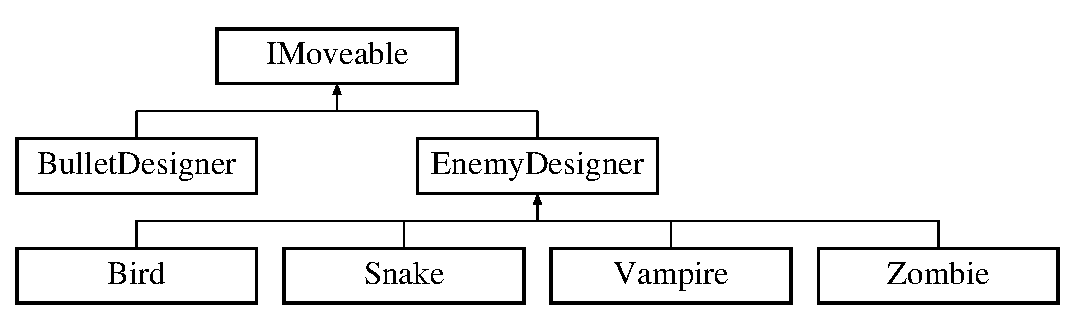
\includegraphics[height=3.000000cm]{class_i_moveable}
\end{center}
\end{figure}
\subsection*{Public Member Functions}
\begin{DoxyCompactItemize}
\item 
\mbox{\Hypertarget{class_i_moveable_a66f241a85348b1c9dba3685f277cf9f7}\label{class_i_moveable_a66f241a85348b1c9dba3685f277cf9f7}} 
virtual uint {\bfseries Get\+Speed} ()=0
\item 
\mbox{\Hypertarget{class_i_moveable_acda53a34a5369a696804afd7f88e63d3}\label{class_i_moveable_acda53a34a5369a696804afd7f88e63d3}} 
virtual void {\bfseries Move} (const \mbox{\hyperlink{class_map}{Map}} \&m, const \mbox{\hyperlink{class_scene}{Scene}} \&scene)=0
\item 
\mbox{\Hypertarget{class_i_moveable_a7b0625b79748c1642e20d95182c42855}\label{class_i_moveable_a7b0625b79748c1642e20d95182c42855}} 
virtual void {\bfseries draw} (sf\+::\+Render\+Target \&target, sf\+::\+Render\+States states)=0
\item 
\mbox{\Hypertarget{class_i_moveable_aa3b73eabadda4deba75d3e2daceb2e67}\label{class_i_moveable_aa3b73eabadda4deba75d3e2daceb2e67}} 
virtual bool {\bfseries Collides} (\mbox{\hyperlink{class_i_moveable}{I\+Moveable}} $\ast$other)=0
\item 
\mbox{\Hypertarget{class_i_moveable_a3e6183140a949499c4e85e4d0d7a771c}\label{class_i_moveable_a3e6183140a949499c4e85e4d0d7a771c}} 
virtual void {\bfseries Collision} (\mbox{\hyperlink{class_i_moveable}{I\+Moveable}} $\ast$other)=0
\item 
\mbox{\Hypertarget{class_i_moveable_a2a8392fa1fe1a22a4f98b2d0ab97a1ff}\label{class_i_moveable_a2a8392fa1fe1a22a4f98b2d0ab97a1ff}} 
virtual sf\+::\+Vector2f {\bfseries Get\+Origin} ()=0
\item 
\mbox{\Hypertarget{class_i_moveable_ade09545d32dc5a0337e15d32ba9f9521}\label{class_i_moveable_ade09545d32dc5a0337e15d32ba9f9521}} 
virtual sf\+::\+Float\+Rect {\bfseries Get\+Rect} ()=0
\item 
\mbox{\Hypertarget{class_i_moveable_ac18bf702bc8c4356f715122270b0e1d5}\label{class_i_moveable_ac18bf702bc8c4356f715122270b0e1d5}} 
virtual bool {\bfseries Removeable} ()=0
\end{DoxyCompactItemize}


\subsection{Detailed Description}
Interface representing the enemy possible actions. 

The documentation for this class was generated from the following file\+:\begin{DoxyCompactItemize}
\item 
Tower\+Defence/\+Graphics\+Handler/Enemy\+Designer.\+h\end{DoxyCompactItemize}

\hypertarget{class_level}{}\section{Level Class Reference}
\label{class_level}\index{Level@{Level}}


Class representing levels in game.  




{\ttfamily \#include $<$Level.\+h$>$}

\subsection*{Public Member Functions}
\begin{DoxyCompactItemize}
\item 
\mbox{\Hypertarget{class_level_a3319abe5123ed42bb6632015656d4df7}\label{class_level_a3319abe5123ed42bb6632015656d4df7}} 
std\+::string \mbox{\hyperlink{class_level_a3319abe5123ed42bb6632015656d4df7}{get\+Map\+Name}} ()
\begin{DoxyCompactList}\small\item\em ~\newline
getter for map name \end{DoxyCompactList}\item 
\mbox{\hyperlink{class_level_ac3219336ec0edadd14e4c8bd012ede11}{Level}} (std\+::vector$<$ \mbox{\hyperlink{class_wave}{Wave}} $>$ vector\+Of\+Waves, std\+::string map\+Name)
\begin{DoxyCompactList}\small\item\em constructor \end{DoxyCompactList}\item 
void \mbox{\hyperlink{class_level_af30bbc6f28d1373854c316a8226503ba}{set\+Map\+Name}} (std\+::string map\+Name)
\begin{DoxyCompactList}\small\item\em setter for map name \end{DoxyCompactList}\item 
void \mbox{\hyperlink{class_level_adc3fb45bf2db8c85e60a6496d8bb5d0c}{set\+Waves}} (std\+::vector$<$ \mbox{\hyperlink{class_wave}{Wave}} $>$ vector\+Of\+Waves)
\begin{DoxyCompactList}\small\item\em setter for map waves \end{DoxyCompactList}\item 
void \mbox{\hyperlink{class_level_a8ffc6f7c57173c9399aa8755b4435353}{clear\+Waves}} ()
\begin{DoxyCompactList}\small\item\em method for clearing vector of waves \end{DoxyCompactList}\item 
\mbox{\Hypertarget{class_level_a7bd752a7575a494d713f6cc548cce015}\label{class_level_a7bd752a7575a494d713f6cc548cce015}} 
std\+::vector$<$ \mbox{\hyperlink{class_wave}{Wave}} $>$ \mbox{\hyperlink{class_level_a7bd752a7575a494d713f6cc548cce015}{get\+Waves}} ()
\begin{DoxyCompactList}\small\item\em ~\newline
getter for waves \end{DoxyCompactList}\item 
void \mbox{\hyperlink{class_level_a1aa9a0d5da3c3a2763620de72c336dcc}{add\+Wave}} (\mbox{\hyperlink{class_wave}{Wave}} wave)
\begin{DoxyCompactList}\small\item\em method for adding waves to vector \end{DoxyCompactList}\end{DoxyCompactItemize}
\subsection*{Protected Attributes}
\begin{DoxyCompactItemize}
\item 
\mbox{\Hypertarget{class_level_abeec0fb04d67ff914e6393bd49d78dc9}\label{class_level_abeec0fb04d67ff914e6393bd49d78dc9}} 
std\+::string {\bfseries map\+Name}
\item 
\mbox{\Hypertarget{class_level_af96606a75a04d4f00a0a426881e6df32}\label{class_level_af96606a75a04d4f00a0a426881e6df32}} 
std\+::vector$<$ \mbox{\hyperlink{class_wave}{Wave}} $>$ {\bfseries vector\+Of\+Waves}
\end{DoxyCompactItemize}


\subsection{Detailed Description}
Class representing levels in game. 

\subsection{Constructor \& Destructor Documentation}
\mbox{\Hypertarget{class_level_ac3219336ec0edadd14e4c8bd012ede11}\label{class_level_ac3219336ec0edadd14e4c8bd012ede11}} 
\index{Level@{Level}!Level@{Level}}
\index{Level@{Level}!Level@{Level}}
\subsubsection{\texorpdfstring{Level()}{Level()}}
{\footnotesize\ttfamily Level\+::\+Level (\begin{DoxyParamCaption}\item[{std\+::vector$<$ \mbox{\hyperlink{class_wave}{Wave}} $>$}]{vector\+Of\+Waves,  }\item[{std\+::string}]{map\+Name }\end{DoxyParamCaption})}



constructor 

Method checks if shoot can be done, i.\+e. checks time interval from last shoot and compares range with distance If shoot is possible, bullet object is created 
\begin{DoxyParams}{Parameters}
{\em vector} & of waves \\
\hline
{\em map\textquotesingle{}s} & name \\
\hline
\end{DoxyParams}


\subsection{Member Function Documentation}
\mbox{\Hypertarget{class_level_a1aa9a0d5da3c3a2763620de72c336dcc}\label{class_level_a1aa9a0d5da3c3a2763620de72c336dcc}} 
\index{Level@{Level}!add\+Wave@{add\+Wave}}
\index{add\+Wave@{add\+Wave}!Level@{Level}}
\subsubsection{\texorpdfstring{add\+Wave()}{addWave()}}
{\footnotesize\ttfamily void Level\+::add\+Wave (\begin{DoxyParamCaption}\item[{\mbox{\hyperlink{class_wave}{Wave}}}]{wave }\end{DoxyParamCaption})}



method for adding waves to vector 

Method adds wave to vector of wave 
\begin{DoxyParams}{Parameters}
{\em \mbox{\hyperlink{class_wave}{Wave}}} & of enemiess \\
\hline
\end{DoxyParams}
\mbox{\Hypertarget{class_level_a8ffc6f7c57173c9399aa8755b4435353}\label{class_level_a8ffc6f7c57173c9399aa8755b4435353}} 
\index{Level@{Level}!clear\+Waves@{clear\+Waves}}
\index{clear\+Waves@{clear\+Waves}!Level@{Level}}
\subsubsection{\texorpdfstring{clear\+Waves()}{clearWaves()}}
{\footnotesize\ttfamily void Level\+::clear\+Waves (\begin{DoxyParamCaption}{ }\end{DoxyParamCaption})}



method for clearing vector of waves 

Method clears vector from current waves \mbox{\Hypertarget{class_level_af30bbc6f28d1373854c316a8226503ba}\label{class_level_af30bbc6f28d1373854c316a8226503ba}} 
\index{Level@{Level}!set\+Map\+Name@{set\+Map\+Name}}
\index{set\+Map\+Name@{set\+Map\+Name}!Level@{Level}}
\subsubsection{\texorpdfstring{set\+Map\+Name()}{setMapName()}}
{\footnotesize\ttfamily void Level\+::set\+Map\+Name (\begin{DoxyParamCaption}\item[{std\+::string}]{map\+Name }\end{DoxyParamCaption})}



setter for map name 


\begin{DoxyParams}{Parameters}
{\em map} & name \\
\hline
\end{DoxyParams}
\mbox{\Hypertarget{class_level_adc3fb45bf2db8c85e60a6496d8bb5d0c}\label{class_level_adc3fb45bf2db8c85e60a6496d8bb5d0c}} 
\index{Level@{Level}!set\+Waves@{set\+Waves}}
\index{set\+Waves@{set\+Waves}!Level@{Level}}
\subsubsection{\texorpdfstring{set\+Waves()}{setWaves()}}
{\footnotesize\ttfamily void Level\+::set\+Waves (\begin{DoxyParamCaption}\item[{std\+::vector$<$ \mbox{\hyperlink{class_wave}{Wave}} $>$}]{vector\+Of\+Waves }\end{DoxyParamCaption})}



setter for map waves 


\begin{DoxyParams}{Parameters}
{\em vector} & of waves \\
\hline
\end{DoxyParams}


The documentation for this class was generated from the following files\+:\begin{DoxyCompactItemize}
\item 
Tower\+Defence/\+Graphics\+Handler/Level.\+h\item 
Tower\+Defence/\+Graphics\+Handler/Level.\+cpp\end{DoxyCompactItemize}

\hypertarget{class_map}{}\section{Map Class Reference}
\label{class_map}\index{Map@{Map}}


Class representing sets of points as a map.  




{\ttfamily \#include $<$Map.\+hpp$>$}

\subsection*{Public Member Functions}
\begin{DoxyCompactItemize}
\item 
\mbox{\hyperlink{class_map_a8497952fd6e1f0584d868e6ceb97d42d}{Map}} (int width, int height)
\begin{DoxyCompactList}\small\item\em constructor \end{DoxyCompactList}\item 
\mbox{\hyperlink{class_map_a953c6ae29b27d415572a016bcf55e768}{Map}} (int width, int height, const int $\ast$int\+Map)
\begin{DoxyCompactList}\small\item\em constructor \end{DoxyCompactList}\item 
bool \mbox{\hyperlink{class_map_a6456ee3beb19614b6ae03a04414d048a}{Set\+Point}} (int x, int y, int new\+Value)
\begin{DoxyCompactList}\small\item\em Method used for setting points with new value Method checks if index of point\textquotesingle{}s is in range, if so-\/it set\textquotesingle{}s terrain with new value and returns true  x dimension  y dimension  new value. \end{DoxyCompactList}\item 
bool \mbox{\hyperlink{class_map_a68903a79aac7c1680b59329ff1b14579}{Set\+Point}} (\mbox{\hyperlink{class_point}{Point}} p, int new\+Value)
\begin{DoxyCompactList}\small\item\em Method used for setting points with new value Method sets map points with logical point x,y and new value  point  new value. \end{DoxyCompactList}\item 
bool \mbox{\hyperlink{class_map_aa1133d277379166a0f4703b6e17849c1}{Set\+Point}} (int x, int y, \mbox{\hyperlink{class_point}{Point}} new\+Point)
\begin{DoxyCompactList}\small\item\em Method used for setting points with new value Method sets map points with new point. it calculates index from x and y and if it is in range-\/it returns true  x  y  new point. \end{DoxyCompactList}\item 
bool \mbox{\hyperlink{class_map_aacc4374e1b3984d54ecbaf9fa488d08e}{Replace\+Point}} (\mbox{\hyperlink{class_point}{Point}} old\+Point, \mbox{\hyperlink{class_point}{Point}} new\+Point)
\begin{DoxyCompactList}\small\item\em Method used for replacing old point with new point  old point  new point replacing old one. \end{DoxyCompactList}\item 
\mbox{\hyperlink{class_point}{Point}} \mbox{\hyperlink{class_map_a9f7239d47a8e426590e98b0fd07c0604}{Get\+Point}} (int x, int y) const
\item 
\mbox{\hyperlink{class_point}{Point}} \mbox{\hyperlink{class_map_aab03ac51e8468984a23f52f3ddd2cbcb}{Get\+Last\+Point}} () const
\begin{DoxyCompactList}\small\item\em getter for last point \end{DoxyCompactList}\item 
int \mbox{\hyperlink{class_map_aeca77ed7c01dec1e8effa05f0e08c266}{Get\+Width}} ()
\begin{DoxyCompactList}\small\item\em getter for map\textquotesingle{}s width \end{DoxyCompactList}\item 
int \mbox{\hyperlink{class_map_a72adf4e41e8e6558e58c2efe20445f7f}{Get\+Height}} ()
\begin{DoxyCompactList}\small\item\em getter for map\textquotesingle{}s height \end{DoxyCompactList}\item 
bool \mbox{\hyperlink{class_map_a20da42fe27ba40a81ebf25947b8a46fc}{Is\+In\+Map}} (\mbox{\hyperlink{class_point}{Point}} p) const
\begin{DoxyCompactList}\small\item\em ~\newline
~\newline
Method used for checking if point is on the map \end{DoxyCompactList}\item 
bool \mbox{\hyperlink{class_map_a7b9c227621696cda01445fdae6a3c80d}{Is\+In\+Map}} (int x, int y) const
\begin{DoxyCompactList}\small\item\em ~\newline
~\newline
Method used for checking if point is on the map \end{DoxyCompactList}\item 
\mbox{\Hypertarget{class_map_aa403fbe09394ccf39747588f5168e3b2}\label{class_map_aa403fbe09394ccf39747588f5168e3b2}} 
\mbox{\hyperlink{class_map_aa403fbe09394ccf39747588f5168e3b2}{$\sim$\+Map}} ()
\begin{DoxyCompactList}\small\item\em destructor \end{DoxyCompactList}\item 
\mbox{\Hypertarget{class_map_a88353e04db090336b830c1353cff7f71}\label{class_map_a88353e04db090336b830c1353cff7f71}} 
void \mbox{\hyperlink{class_map_a88353e04db090336b830c1353cff7f71}{Display}} () const
\begin{DoxyCompactList}\small\item\em Method used for displaying information about point on std output. \end{DoxyCompactList}\end{DoxyCompactItemize}


\subsection{Detailed Description}
Class representing sets of points as a map. 

\subsection{Constructor \& Destructor Documentation}
\mbox{\Hypertarget{class_map_a8497952fd6e1f0584d868e6ceb97d42d}\label{class_map_a8497952fd6e1f0584d868e6ceb97d42d}} 
\index{Map@{Map}!Map@{Map}}
\index{Map@{Map}!Map@{Map}}
\subsubsection{\texorpdfstring{Map()}{Map()}\hspace{0.1cm}{\footnotesize\ttfamily [1/2]}}
{\footnotesize\ttfamily Map\+::\+Map (\begin{DoxyParamCaption}\item[{int}]{width,  }\item[{int}]{height }\end{DoxyParamCaption})\hspace{0.3cm}{\ttfamily [explicit]}}



constructor 

map\textquotesingle{}s width  map\textquotesingle{}s height \mbox{\Hypertarget{class_map_a953c6ae29b27d415572a016bcf55e768}\label{class_map_a953c6ae29b27d415572a016bcf55e768}} 
\index{Map@{Map}!Map@{Map}}
\index{Map@{Map}!Map@{Map}}
\subsubsection{\texorpdfstring{Map()}{Map()}\hspace{0.1cm}{\footnotesize\ttfamily [2/2]}}
{\footnotesize\ttfamily Map\+::\+Map (\begin{DoxyParamCaption}\item[{int}]{width,  }\item[{int}]{height,  }\item[{const int $\ast$}]{int\+Map }\end{DoxyParamCaption})\hspace{0.3cm}{\ttfamily [explicit]}}



constructor 


\begin{DoxyParams}{Parameters}
{\em map\textquotesingle{}s} & width \\
\hline
{\em map\textquotesingle{}s} & height \\
\hline
{\em pointer} & used for map initialization \\
\hline
\end{DoxyParams}


\subsection{Member Function Documentation}
\mbox{\Hypertarget{class_map_a72adf4e41e8e6558e58c2efe20445f7f}\label{class_map_a72adf4e41e8e6558e58c2efe20445f7f}} 
\index{Map@{Map}!Get\+Height@{Get\+Height}}
\index{Get\+Height@{Get\+Height}!Map@{Map}}
\subsubsection{\texorpdfstring{Get\+Height()}{GetHeight()}}
{\footnotesize\ttfamily int Map\+::\+Get\+Height (\begin{DoxyParamCaption}{ }\end{DoxyParamCaption})}



getter for map\textquotesingle{}s height 

\begin{DoxyReturn}{Returns}
map\textquotesingle{}s height 
\end{DoxyReturn}
\mbox{\Hypertarget{class_map_aab03ac51e8468984a23f52f3ddd2cbcb}\label{class_map_aab03ac51e8468984a23f52f3ddd2cbcb}} 
\index{Map@{Map}!Get\+Last\+Point@{Get\+Last\+Point}}
\index{Get\+Last\+Point@{Get\+Last\+Point}!Map@{Map}}
\subsubsection{\texorpdfstring{Get\+Last\+Point()}{GetLastPoint()}}
{\footnotesize\ttfamily \mbox{\hyperlink{class_point}{Point}} Map\+::\+Get\+Last\+Point (\begin{DoxyParamCaption}{ }\end{DoxyParamCaption}) const}



getter for last point 

\begin{DoxyReturn}{Returns}
last point in collection 
\end{DoxyReturn}
\mbox{\Hypertarget{class_map_a9f7239d47a8e426590e98b0fd07c0604}\label{class_map_a9f7239d47a8e426590e98b0fd07c0604}} 
\index{Map@{Map}!Get\+Point@{Get\+Point}}
\index{Get\+Point@{Get\+Point}!Map@{Map}}
\subsubsection{\texorpdfstring{Get\+Point()}{GetPoint()}}
{\footnotesize\ttfamily \mbox{\hyperlink{class_point}{Point}} Map\+::\+Get\+Point (\begin{DoxyParamCaption}\item[{int}]{x,  }\item[{int}]{y }\end{DoxyParamCaption}) const}

Important\+: In case of invalid coordinates, function returns point (x=-\/1, y=-\/1, value=-\/1) which is incorrect point in map. Use Is\+In\+Map function before invoking this. \mbox{\Hypertarget{class_map_aeca77ed7c01dec1e8effa05f0e08c266}\label{class_map_aeca77ed7c01dec1e8effa05f0e08c266}} 
\index{Map@{Map}!Get\+Width@{Get\+Width}}
\index{Get\+Width@{Get\+Width}!Map@{Map}}
\subsubsection{\texorpdfstring{Get\+Width()}{GetWidth()}}
{\footnotesize\ttfamily int Map\+::\+Get\+Width (\begin{DoxyParamCaption}{ }\end{DoxyParamCaption})}



getter for map\textquotesingle{}s width 

\begin{DoxyReturn}{Returns}
map\textquotesingle{}s width 
\end{DoxyReturn}
\mbox{\Hypertarget{class_map_a20da42fe27ba40a81ebf25947b8a46fc}\label{class_map_a20da42fe27ba40a81ebf25947b8a46fc}} 
\index{Map@{Map}!Is\+In\+Map@{Is\+In\+Map}}
\index{Is\+In\+Map@{Is\+In\+Map}!Map@{Map}}
\subsubsection{\texorpdfstring{Is\+In\+Map()}{IsInMap()}\hspace{0.1cm}{\footnotesize\ttfamily [1/2]}}
{\footnotesize\ttfamily bool Map\+::\+Is\+In\+Map (\begin{DoxyParamCaption}\item[{\mbox{\hyperlink{class_point}{Point}}}]{p }\end{DoxyParamCaption}) const}



~\newline
~\newline
Method used for checking if point is on the map 

\begin{DoxyReturn}{Returns}
false if point(x,y) is not on the map 
\end{DoxyReturn}
\mbox{\Hypertarget{class_map_a7b9c227621696cda01445fdae6a3c80d}\label{class_map_a7b9c227621696cda01445fdae6a3c80d}} 
\index{Map@{Map}!Is\+In\+Map@{Is\+In\+Map}}
\index{Is\+In\+Map@{Is\+In\+Map}!Map@{Map}}
\subsubsection{\texorpdfstring{Is\+In\+Map()}{IsInMap()}\hspace{0.1cm}{\footnotesize\ttfamily [2/2]}}
{\footnotesize\ttfamily bool Map\+::\+Is\+In\+Map (\begin{DoxyParamCaption}\item[{int}]{x,  }\item[{int}]{y }\end{DoxyParamCaption}) const}



~\newline
~\newline
Method used for checking if point is on the map 

\begin{DoxyReturn}{Returns}
false if point(x,y) is not on the map 
\end{DoxyReturn}
\mbox{\Hypertarget{class_map_aacc4374e1b3984d54ecbaf9fa488d08e}\label{class_map_aacc4374e1b3984d54ecbaf9fa488d08e}} 
\index{Map@{Map}!Replace\+Point@{Replace\+Point}}
\index{Replace\+Point@{Replace\+Point}!Map@{Map}}
\subsubsection{\texorpdfstring{Replace\+Point()}{ReplacePoint()}}
{\footnotesize\ttfamily bool Map\+::\+Replace\+Point (\begin{DoxyParamCaption}\item[{\mbox{\hyperlink{class_point}{Point}}}]{old\+Point,  }\item[{\mbox{\hyperlink{class_point}{Point}}}]{new\+Point }\end{DoxyParamCaption})}



Method used for replacing old point with new point  old point  new point replacing old one. 

\begin{DoxyReturn}{Returns}
true if points was set successfully 
\end{DoxyReturn}
\mbox{\Hypertarget{class_map_a6456ee3beb19614b6ae03a04414d048a}\label{class_map_a6456ee3beb19614b6ae03a04414d048a}} 
\index{Map@{Map}!Set\+Point@{Set\+Point}}
\index{Set\+Point@{Set\+Point}!Map@{Map}}
\subsubsection{\texorpdfstring{Set\+Point()}{SetPoint()}\hspace{0.1cm}{\footnotesize\ttfamily [1/3]}}
{\footnotesize\ttfamily bool Map\+::\+Set\+Point (\begin{DoxyParamCaption}\item[{int}]{x,  }\item[{int}]{y,  }\item[{int}]{new\+Value }\end{DoxyParamCaption})}



Method used for setting points with new value Method checks if index of point\textquotesingle{}s is in range, if so-\/it set\textquotesingle{}s terrain with new value and returns true  x dimension  y dimension  new value. 

\begin{DoxyReturn}{Returns}
true if index is in range 
\end{DoxyReturn}
\mbox{\Hypertarget{class_map_a68903a79aac7c1680b59329ff1b14579}\label{class_map_a68903a79aac7c1680b59329ff1b14579}} 
\index{Map@{Map}!Set\+Point@{Set\+Point}}
\index{Set\+Point@{Set\+Point}!Map@{Map}}
\subsubsection{\texorpdfstring{Set\+Point()}{SetPoint()}\hspace{0.1cm}{\footnotesize\ttfamily [2/3]}}
{\footnotesize\ttfamily bool Map\+::\+Set\+Point (\begin{DoxyParamCaption}\item[{\mbox{\hyperlink{class_point}{Point}}}]{p,  }\item[{int}]{new\+Value }\end{DoxyParamCaption})}



Method used for setting points with new value Method sets map points with logical point x,y and new value  point  new value. 

\begin{DoxyReturn}{Returns}
true if point was in range 
\end{DoxyReturn}
\mbox{\Hypertarget{class_map_aa1133d277379166a0f4703b6e17849c1}\label{class_map_aa1133d277379166a0f4703b6e17849c1}} 
\index{Map@{Map}!Set\+Point@{Set\+Point}}
\index{Set\+Point@{Set\+Point}!Map@{Map}}
\subsubsection{\texorpdfstring{Set\+Point()}{SetPoint()}\hspace{0.1cm}{\footnotesize\ttfamily [3/3]}}
{\footnotesize\ttfamily bool Map\+::\+Set\+Point (\begin{DoxyParamCaption}\item[{int}]{x,  }\item[{int}]{y,  }\item[{\mbox{\hyperlink{class_point}{Point}}}]{new\+Point }\end{DoxyParamCaption})}



Method used for setting points with new value Method sets map points with new point. it calculates index from x and y and if it is in range-\/it returns true  x  y  new point. 

\begin{DoxyReturn}{Returns}
true if index is in range 
\end{DoxyReturn}


The documentation for this class was generated from the following files\+:\begin{DoxyCompactItemize}
\item 
Tower\+Defence/\+Graphics\+Handler/Map.\+hpp\item 
Tower\+Defence/\+Graphics\+Handler/Map.\+cpp\end{DoxyCompactItemize}

\hypertarget{class_map_file_parser}{}\section{Map\+File\+Parser Class Reference}
\label{class_map_file_parser}\index{Map\+File\+Parser@{Map\+File\+Parser}}


Class used for parsing file containing map\textquotesingle{}s settings.  




{\ttfamily \#include $<$Map.\+hpp$>$}

\subsection*{Public Member Functions}
\begin{DoxyCompactItemize}
\item 
bool \mbox{\hyperlink{class_map_file_parser_a763133f44741dc4164595d03df036d0b}{Parse\+File}} ()
\begin{DoxyCompactList}\small\item\em method used for parsing file \end{DoxyCompactList}\item 
\mbox{\hyperlink{class_map_file_parser_a650246d5b95af369b885615c6b7d61bf}{Map\+File\+Parser}} (std\+::string s\+File\+Path)
\begin{DoxyCompactList}\small\item\em constructor of file parser \end{DoxyCompactList}\item 
\mbox{\hyperlink{class_map}{Map}} \mbox{\hyperlink{class_map_file_parser_a4c6fa40ab985db21869eecdcdba62549}{parsed\+Map}} ()
\begin{DoxyCompactList}\small\item\em getter for parsed map \end{DoxyCompactList}\item 
\mbox{\Hypertarget{class_map_file_parser_a897daf88843f2c6ce2549ccc22f932b9}\label{class_map_file_parser_a897daf88843f2c6ce2549ccc22f932b9}} 
\mbox{\hyperlink{class_map_file_parser_a897daf88843f2c6ce2549ccc22f932b9}{$\sim$\+Map\+File\+Parser}} ()
\begin{DoxyCompactList}\small\item\em destructor \end{DoxyCompactList}\end{DoxyCompactItemize}


\subsection{Detailed Description}
Class used for parsing file containing map\textquotesingle{}s settings. 

\subsection{Constructor \& Destructor Documentation}
\mbox{\Hypertarget{class_map_file_parser_a650246d5b95af369b885615c6b7d61bf}\label{class_map_file_parser_a650246d5b95af369b885615c6b7d61bf}} 
\index{Map\+File\+Parser@{Map\+File\+Parser}!Map\+File\+Parser@{Map\+File\+Parser}}
\index{Map\+File\+Parser@{Map\+File\+Parser}!Map\+File\+Parser@{Map\+File\+Parser}}
\subsubsection{\texorpdfstring{Map\+File\+Parser()}{MapFileParser()}}
{\footnotesize\ttfamily Map\+File\+Parser\+::\+Map\+File\+Parser (\begin{DoxyParamCaption}\item[{std\+::string}]{s\+File\+Path }\end{DoxyParamCaption})\hspace{0.3cm}{\ttfamily [explicit]}}



constructor of file parser 


\begin{DoxyParams}{Parameters}
{\em filename} & \\
\hline
\end{DoxyParams}


\subsection{Member Function Documentation}
\mbox{\Hypertarget{class_map_file_parser_a4c6fa40ab985db21869eecdcdba62549}\label{class_map_file_parser_a4c6fa40ab985db21869eecdcdba62549}} 
\index{Map\+File\+Parser@{Map\+File\+Parser}!parsed\+Map@{parsed\+Map}}
\index{parsed\+Map@{parsed\+Map}!Map\+File\+Parser@{Map\+File\+Parser}}
\subsubsection{\texorpdfstring{parsed\+Map()}{parsedMap()}}
{\footnotesize\ttfamily \mbox{\hyperlink{class_map}{Map}} Map\+File\+Parser\+::parsed\+Map (\begin{DoxyParamCaption}{ }\end{DoxyParamCaption})}



getter for parsed map 

\begin{DoxyReturn}{Returns}
\mbox{\hyperlink{class_map}{Map}} 
\end{DoxyReturn}

\begin{DoxyExceptions}{Exceptions}
{\em \mbox{\hyperlink{class_custom_exception}{Custom\+Exception}}} & indicating that file wasn\textquotesingle{}t successfully read \\
\hline
\end{DoxyExceptions}
\mbox{\Hypertarget{class_map_file_parser_a763133f44741dc4164595d03df036d0b}\label{class_map_file_parser_a763133f44741dc4164595d03df036d0b}} 
\index{Map\+File\+Parser@{Map\+File\+Parser}!Parse\+File@{Parse\+File}}
\index{Parse\+File@{Parse\+File}!Map\+File\+Parser@{Map\+File\+Parser}}
\subsubsection{\texorpdfstring{Parse\+File()}{ParseFile()}}
{\footnotesize\ttfamily bool Map\+File\+Parser\+::\+Parse\+File (\begin{DoxyParamCaption}{ }\end{DoxyParamCaption})}



method used for parsing file 

\begin{DoxyReturn}{Returns}
logical indicating whether reading map and dimensions were succesfull 
\end{DoxyReturn}


The documentation for this class was generated from the following files\+:\begin{DoxyCompactItemize}
\item 
Tower\+Defence/\+Graphics\+Handler/Map.\+hpp\item 
Tower\+Defence/\+Graphics\+Handler/Map.\+cpp\end{DoxyCompactItemize}

\hypertarget{classrapidxml_1_1memory__pool}{}\section{rapidxml\+:\+:memory\+\_\+pool$<$ Ch $>$ Class Template Reference}
\label{classrapidxml_1_1memory__pool}\index{rapidxml\+::memory\+\_\+pool$<$ Ch $>$@{rapidxml\+::memory\+\_\+pool$<$ Ch $>$}}


{\ttfamily \#include $<$rapidxml.\+hpp$>$}

Inheritance diagram for rapidxml\+:\+:memory\+\_\+pool$<$ Ch $>$\+:\begin{figure}[H]
\begin{center}
\leavevmode
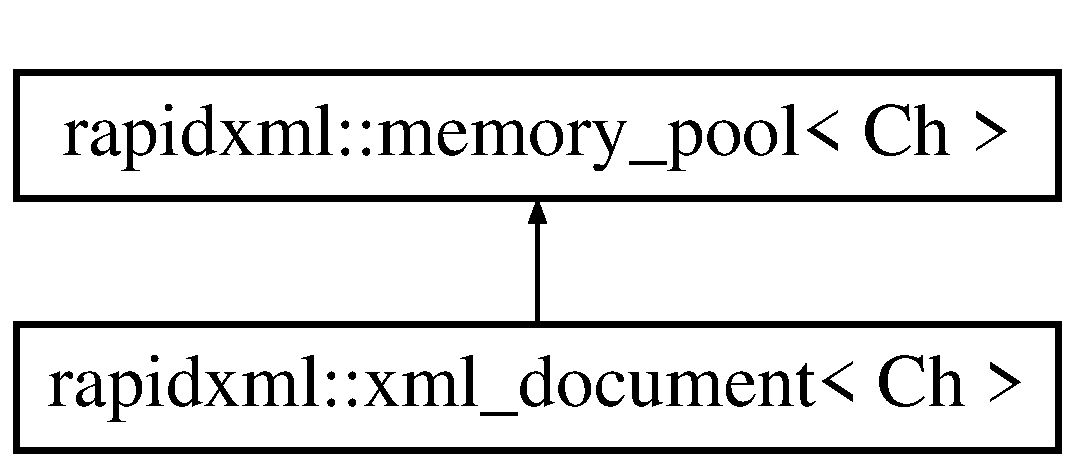
\includegraphics[height=2.000000cm]{classrapidxml_1_1memory__pool}
\end{center}
\end{figure}
\subsection*{Public Member Functions}
\begin{DoxyCompactItemize}
\item 
\mbox{\Hypertarget{classrapidxml_1_1memory__pool_a0b609da81dff28a19ebd704400788429}\label{classrapidxml_1_1memory__pool_a0b609da81dff28a19ebd704400788429}} 
\mbox{\hyperlink{classrapidxml_1_1memory__pool_a0b609da81dff28a19ebd704400788429}{memory\+\_\+pool}} ()
\begin{DoxyCompactList}\small\item\em Constructs empty pool with default allocator functions. \end{DoxyCompactList}\item 
\mbox{\hyperlink{classrapidxml_1_1memory__pool_a0a3e82126e59e4077f41e933130bb5a0}{$\sim$memory\+\_\+pool}} ()
\item 
\mbox{\hyperlink{classrapidxml_1_1xml__node}{xml\+\_\+node}}$<$ Ch $>$ $\ast$ \mbox{\hyperlink{classrapidxml_1_1memory__pool_a4118581c29ee9a2f6b55ebf7dac185f8}{allocate\+\_\+node}} (\mbox{\hyperlink{rapidxml_8hpp_abb456db38f7efb746c4330eed6072a7c}{node\+\_\+type}} type, const Ch $\ast$name=0, const Ch $\ast$value=0, std\+::size\+\_\+t name\+\_\+size=0, std\+::size\+\_\+t value\+\_\+size=0)
\item 
\mbox{\hyperlink{classrapidxml_1_1xml__attribute}{xml\+\_\+attribute}}$<$ Ch $>$ $\ast$ \mbox{\hyperlink{classrapidxml_1_1memory__pool_a3de2a66c983336e006ea3844e244ed30}{allocate\+\_\+attribute}} (const Ch $\ast$name=0, const Ch $\ast$value=0, std\+::size\+\_\+t name\+\_\+size=0, std\+::size\+\_\+t value\+\_\+size=0)
\item 
Ch $\ast$ \mbox{\hyperlink{classrapidxml_1_1memory__pool_a171941b39d55b868358da97462185f58}{allocate\+\_\+string}} (const Ch $\ast$source=0, std\+::size\+\_\+t size=0)
\item 
\mbox{\hyperlink{classrapidxml_1_1xml__node}{xml\+\_\+node}}$<$ Ch $>$ $\ast$ \mbox{\hyperlink{classrapidxml_1_1memory__pool_a0a10679fc17597d339a0dc107f8a94ac}{clone\+\_\+node}} (const \mbox{\hyperlink{classrapidxml_1_1xml__node}{xml\+\_\+node}}$<$ Ch $>$ $\ast$source, \mbox{\hyperlink{classrapidxml_1_1xml__node}{xml\+\_\+node}}$<$ Ch $>$ $\ast$result=0)
\item 
void \mbox{\hyperlink{classrapidxml_1_1memory__pool_aad377c835fdaed1cb2cc9df194cf84e4}{clear}} ()
\item 
void \mbox{\hyperlink{classrapidxml_1_1memory__pool_a84d3d8d2cdfc00501e1dcf26d889ae03}{set\+\_\+allocator}} (alloc\+\_\+func $\ast$af, free\+\_\+func $\ast$ff)
\end{DoxyCompactItemize}


\subsection{Detailed Description}
\subsubsection*{template$<$class Ch = char$>$\newline
class rapidxml\+::memory\+\_\+pool$<$ Ch $>$}

This class is used by the parser to create new nodes and attributes, without overheads of dynamic memory allocation. In most cases, you will not need to use this class directly. However, if you need to create nodes manually or modify names/values of nodes, you are encouraged to use \mbox{\hyperlink{classrapidxml_1_1memory__pool}{memory\+\_\+pool}} of relevant \mbox{\hyperlink{classrapidxml_1_1xml__document}{xml\+\_\+document}} to allocate the memory. Not only is this faster than allocating them by using {\ttfamily new} operator, but also their lifetime will be tied to the lifetime of document, possibly simplyfing memory management. ~\newline
~\newline
 Call \mbox{\hyperlink{classrapidxml_1_1memory__pool_a4118581c29ee9a2f6b55ebf7dac185f8}{allocate\+\_\+node()}} or \mbox{\hyperlink{classrapidxml_1_1memory__pool_a3de2a66c983336e006ea3844e244ed30}{allocate\+\_\+attribute()}} functions to obtain new nodes or attributes from the pool. You can also call \mbox{\hyperlink{classrapidxml_1_1memory__pool_a171941b39d55b868358da97462185f58}{allocate\+\_\+string()}} function to allocate strings. Such strings can then be used as names or values of nodes without worrying about their lifetime. Note that there is no {\ttfamily free()} function -- all allocations are freed at once when \mbox{\hyperlink{classrapidxml_1_1memory__pool_aad377c835fdaed1cb2cc9df194cf84e4}{clear()}} function is called, or when the pool is destroyed. ~\newline
~\newline
 It is also possible to create a standalone \mbox{\hyperlink{classrapidxml_1_1memory__pool}{memory\+\_\+pool}}, and use it to allocate nodes, whose lifetime will not be tied to any document. ~\newline
~\newline
 Pool maintains {\ttfamily R\+A\+P\+I\+D\+X\+M\+L\+\_\+\+S\+T\+A\+T\+I\+C\+\_\+\+P\+O\+O\+L\+\_\+\+S\+I\+ZE} bytes of statically allocated memory. Until static memory is exhausted, no dynamic memory allocations are done. When static memory is exhausted, pool allocates additional blocks of memory of size {\ttfamily R\+A\+P\+I\+D\+X\+M\+L\+\_\+\+D\+Y\+N\+A\+M\+I\+C\+\_\+\+P\+O\+O\+L\+\_\+\+S\+I\+ZE} each, by using global {\ttfamily new\mbox{[}\mbox{]}} and {\ttfamily delete\mbox{[}\mbox{]}} operators. This behaviour can be changed by setting custom allocation routines. Use \mbox{\hyperlink{classrapidxml_1_1memory__pool_a84d3d8d2cdfc00501e1dcf26d889ae03}{set\+\_\+allocator()}} function to set them. ~\newline
~\newline
 Allocations for nodes, attributes and strings are aligned at {\ttfamily R\+A\+P\+I\+D\+X\+M\+L\+\_\+\+A\+L\+I\+G\+N\+M\+E\+NT} bytes. This value defaults to the size of pointer on target architecture. ~\newline
~\newline
 To obtain absolutely top performance from the parser, it is important that all nodes are allocated from a single, contiguous block of memory. Otherwise, cache misses when jumping between two (or more) disjoint blocks of memory can slow down parsing quite considerably. If required, you can tweak {\ttfamily R\+A\+P\+I\+D\+X\+M\+L\+\_\+\+S\+T\+A\+T\+I\+C\+\_\+\+P\+O\+O\+L\+\_\+\+S\+I\+ZE}, {\ttfamily R\+A\+P\+I\+D\+X\+M\+L\+\_\+\+D\+Y\+N\+A\+M\+I\+C\+\_\+\+P\+O\+O\+L\+\_\+\+S\+I\+ZE} and {\ttfamily R\+A\+P\+I\+D\+X\+M\+L\+\_\+\+A\+L\+I\+G\+N\+M\+E\+NT} to obtain best wasted memory to performance compromise. To do it, define their values before \mbox{\hyperlink{rapidxml_8hpp}{rapidxml.\+hpp}} file is included. 
\begin{DoxyParams}{Parameters}
{\em Ch} & Character type of created nodes. \\
\hline
\end{DoxyParams}


\subsection{Constructor \& Destructor Documentation}
\mbox{\Hypertarget{classrapidxml_1_1memory__pool_a0a3e82126e59e4077f41e933130bb5a0}\label{classrapidxml_1_1memory__pool_a0a3e82126e59e4077f41e933130bb5a0}} 
\index{rapidxml\+::memory\+\_\+pool@{rapidxml\+::memory\+\_\+pool}!````~memory\+\_\+pool@{$\sim$memory\+\_\+pool}}
\index{````~memory\+\_\+pool@{$\sim$memory\+\_\+pool}!rapidxml\+::memory\+\_\+pool@{rapidxml\+::memory\+\_\+pool}}
\subsubsection{\texorpdfstring{$\sim$memory\+\_\+pool()}{~memory\_pool()}}
{\footnotesize\ttfamily template$<$class Ch  = char$>$ \\
\mbox{\hyperlink{classrapidxml_1_1memory__pool}{rapidxml\+::memory\+\_\+pool}}$<$ Ch $>$\+::$\sim$\mbox{\hyperlink{classrapidxml_1_1memory__pool}{memory\+\_\+pool}} (\begin{DoxyParamCaption}{ }\end{DoxyParamCaption})\hspace{0.3cm}{\ttfamily [inline]}}

Destroys pool and frees all the memory. This causes memory occupied by nodes allocated by the pool to be freed. Nodes allocated from the pool are no longer valid. 

\subsection{Member Function Documentation}
\mbox{\Hypertarget{classrapidxml_1_1memory__pool_a3de2a66c983336e006ea3844e244ed30}\label{classrapidxml_1_1memory__pool_a3de2a66c983336e006ea3844e244ed30}} 
\index{rapidxml\+::memory\+\_\+pool@{rapidxml\+::memory\+\_\+pool}!allocate\+\_\+attribute@{allocate\+\_\+attribute}}
\index{allocate\+\_\+attribute@{allocate\+\_\+attribute}!rapidxml\+::memory\+\_\+pool@{rapidxml\+::memory\+\_\+pool}}
\subsubsection{\texorpdfstring{allocate\+\_\+attribute()}{allocate\_attribute()}}
{\footnotesize\ttfamily template$<$class Ch  = char$>$ \\
\mbox{\hyperlink{classrapidxml_1_1xml__attribute}{xml\+\_\+attribute}}$<$Ch$>$$\ast$ \mbox{\hyperlink{classrapidxml_1_1memory__pool}{rapidxml\+::memory\+\_\+pool}}$<$ Ch $>$\+::allocate\+\_\+attribute (\begin{DoxyParamCaption}\item[{const Ch $\ast$}]{name = {\ttfamily 0},  }\item[{const Ch $\ast$}]{value = {\ttfamily 0},  }\item[{std\+::size\+\_\+t}]{name\+\_\+size = {\ttfamily 0},  }\item[{std\+::size\+\_\+t}]{value\+\_\+size = {\ttfamily 0} }\end{DoxyParamCaption})\hspace{0.3cm}{\ttfamily [inline]}}

Allocates a new attribute from the pool, and optionally assigns name and value to it. If the allocation request cannot be accomodated, this function will throw {\ttfamily std\+::bad\+\_\+alloc}. If exceptions are disabled by defining R\+A\+P\+I\+D\+X\+M\+L\+\_\+\+N\+O\+\_\+\+E\+X\+C\+E\+P\+T\+I\+O\+NS, this function will call rapidxml\+::parse\+\_\+error\+\_\+handler() function. 
\begin{DoxyParams}{Parameters}
{\em name} & Name to assign to the attribute, or 0 to assign no name. \\
\hline
{\em value} & Value to assign to the attribute, or 0 to assign no value. \\
\hline
{\em name\+\_\+size} & Size of name to assign, or 0 to automatically calculate size from name string. \\
\hline
{\em value\+\_\+size} & Size of value to assign, or 0 to automatically calculate size from value string. \\
\hline
\end{DoxyParams}
\begin{DoxyReturn}{Returns}
Pointer to allocated attribute. This pointer will never be N\+U\+LL. 
\end{DoxyReturn}
\mbox{\Hypertarget{classrapidxml_1_1memory__pool_a4118581c29ee9a2f6b55ebf7dac185f8}\label{classrapidxml_1_1memory__pool_a4118581c29ee9a2f6b55ebf7dac185f8}} 
\index{rapidxml\+::memory\+\_\+pool@{rapidxml\+::memory\+\_\+pool}!allocate\+\_\+node@{allocate\+\_\+node}}
\index{allocate\+\_\+node@{allocate\+\_\+node}!rapidxml\+::memory\+\_\+pool@{rapidxml\+::memory\+\_\+pool}}
\subsubsection{\texorpdfstring{allocate\+\_\+node()}{allocate\_node()}}
{\footnotesize\ttfamily template$<$class Ch  = char$>$ \\
\mbox{\hyperlink{classrapidxml_1_1xml__node}{xml\+\_\+node}}$<$Ch$>$$\ast$ \mbox{\hyperlink{classrapidxml_1_1memory__pool}{rapidxml\+::memory\+\_\+pool}}$<$ Ch $>$\+::allocate\+\_\+node (\begin{DoxyParamCaption}\item[{\mbox{\hyperlink{rapidxml_8hpp_abb456db38f7efb746c4330eed6072a7c}{node\+\_\+type}}}]{type,  }\item[{const Ch $\ast$}]{name = {\ttfamily 0},  }\item[{const Ch $\ast$}]{value = {\ttfamily 0},  }\item[{std\+::size\+\_\+t}]{name\+\_\+size = {\ttfamily 0},  }\item[{std\+::size\+\_\+t}]{value\+\_\+size = {\ttfamily 0} }\end{DoxyParamCaption})\hspace{0.3cm}{\ttfamily [inline]}}

Allocates a new node from the pool, and optionally assigns name and value to it. If the allocation request cannot be accomodated, this function will throw {\ttfamily std\+::bad\+\_\+alloc}. If exceptions are disabled by defining R\+A\+P\+I\+D\+X\+M\+L\+\_\+\+N\+O\+\_\+\+E\+X\+C\+E\+P\+T\+I\+O\+NS, this function will call rapidxml\+::parse\+\_\+error\+\_\+handler() function. 
\begin{DoxyParams}{Parameters}
{\em type} & Type of node to create. \\
\hline
{\em name} & Name to assign to the node, or 0 to assign no name. \\
\hline
{\em value} & Value to assign to the node, or 0 to assign no value. \\
\hline
{\em name\+\_\+size} & Size of name to assign, or 0 to automatically calculate size from name string. \\
\hline
{\em value\+\_\+size} & Size of value to assign, or 0 to automatically calculate size from value string. \\
\hline
\end{DoxyParams}
\begin{DoxyReturn}{Returns}
Pointer to allocated node. This pointer will never be N\+U\+LL. 
\end{DoxyReturn}
\mbox{\Hypertarget{classrapidxml_1_1memory__pool_a171941b39d55b868358da97462185f58}\label{classrapidxml_1_1memory__pool_a171941b39d55b868358da97462185f58}} 
\index{rapidxml\+::memory\+\_\+pool@{rapidxml\+::memory\+\_\+pool}!allocate\+\_\+string@{allocate\+\_\+string}}
\index{allocate\+\_\+string@{allocate\+\_\+string}!rapidxml\+::memory\+\_\+pool@{rapidxml\+::memory\+\_\+pool}}
\subsubsection{\texorpdfstring{allocate\+\_\+string()}{allocate\_string()}}
{\footnotesize\ttfamily template$<$class Ch  = char$>$ \\
Ch$\ast$ \mbox{\hyperlink{classrapidxml_1_1memory__pool}{rapidxml\+::memory\+\_\+pool}}$<$ Ch $>$\+::allocate\+\_\+string (\begin{DoxyParamCaption}\item[{const Ch $\ast$}]{source = {\ttfamily 0},  }\item[{std\+::size\+\_\+t}]{size = {\ttfamily 0} }\end{DoxyParamCaption})\hspace{0.3cm}{\ttfamily [inline]}}

Allocates a char array of given size from the pool, and optionally copies a given string to it. If the allocation request cannot be accomodated, this function will throw {\ttfamily std\+::bad\+\_\+alloc}. If exceptions are disabled by defining R\+A\+P\+I\+D\+X\+M\+L\+\_\+\+N\+O\+\_\+\+E\+X\+C\+E\+P\+T\+I\+O\+NS, this function will call rapidxml\+::parse\+\_\+error\+\_\+handler() function. 
\begin{DoxyParams}{Parameters}
{\em source} & String to initialize the allocated memory with, or 0 to not initialize it. \\
\hline
{\em size} & Number of characters to allocate, or zero to calculate it automatically from source string length; if size is 0, source string must be specified and null terminated. \\
\hline
\end{DoxyParams}
\begin{DoxyReturn}{Returns}
Pointer to allocated char array. This pointer will never be N\+U\+LL. 
\end{DoxyReturn}
\mbox{\Hypertarget{classrapidxml_1_1memory__pool_aad377c835fdaed1cb2cc9df194cf84e4}\label{classrapidxml_1_1memory__pool_aad377c835fdaed1cb2cc9df194cf84e4}} 
\index{rapidxml\+::memory\+\_\+pool@{rapidxml\+::memory\+\_\+pool}!clear@{clear}}
\index{clear@{clear}!rapidxml\+::memory\+\_\+pool@{rapidxml\+::memory\+\_\+pool}}
\subsubsection{\texorpdfstring{clear()}{clear()}}
{\footnotesize\ttfamily template$<$class Ch  = char$>$ \\
void \mbox{\hyperlink{classrapidxml_1_1memory__pool}{rapidxml\+::memory\+\_\+pool}}$<$ Ch $>$\+::clear (\begin{DoxyParamCaption}{ }\end{DoxyParamCaption})\hspace{0.3cm}{\ttfamily [inline]}}

Clears the pool. This causes memory occupied by nodes allocated by the pool to be freed. Any nodes or strings allocated from the pool will no longer be valid. \mbox{\Hypertarget{classrapidxml_1_1memory__pool_a0a10679fc17597d339a0dc107f8a94ac}\label{classrapidxml_1_1memory__pool_a0a10679fc17597d339a0dc107f8a94ac}} 
\index{rapidxml\+::memory\+\_\+pool@{rapidxml\+::memory\+\_\+pool}!clone\+\_\+node@{clone\+\_\+node}}
\index{clone\+\_\+node@{clone\+\_\+node}!rapidxml\+::memory\+\_\+pool@{rapidxml\+::memory\+\_\+pool}}
\subsubsection{\texorpdfstring{clone\+\_\+node()}{clone\_node()}}
{\footnotesize\ttfamily template$<$class Ch  = char$>$ \\
\mbox{\hyperlink{classrapidxml_1_1xml__node}{xml\+\_\+node}}$<$Ch$>$$\ast$ \mbox{\hyperlink{classrapidxml_1_1memory__pool}{rapidxml\+::memory\+\_\+pool}}$<$ Ch $>$\+::clone\+\_\+node (\begin{DoxyParamCaption}\item[{const \mbox{\hyperlink{classrapidxml_1_1xml__node}{xml\+\_\+node}}$<$ Ch $>$ $\ast$}]{source,  }\item[{\mbox{\hyperlink{classrapidxml_1_1xml__node}{xml\+\_\+node}}$<$ Ch $>$ $\ast$}]{result = {\ttfamily 0} }\end{DoxyParamCaption})\hspace{0.3cm}{\ttfamily [inline]}}

Clones an \mbox{\hyperlink{classrapidxml_1_1xml__node}{xml\+\_\+node}} and its hierarchy of child nodes and attributes. Nodes and attributes are allocated from this memory pool. Names and values are not cloned, they are shared between the clone and the source. Result node can be optionally specified as a second parameter, in which case its contents will be replaced with cloned source node. This is useful when you want to clone entire document. 
\begin{DoxyParams}{Parameters}
{\em source} & Node to clone. \\
\hline
{\em result} & Node to put results in, or 0 to automatically allocate result node \\
\hline
\end{DoxyParams}
\begin{DoxyReturn}{Returns}
Pointer to cloned node. This pointer will never be N\+U\+LL. 
\end{DoxyReturn}
\mbox{\Hypertarget{classrapidxml_1_1memory__pool_a84d3d8d2cdfc00501e1dcf26d889ae03}\label{classrapidxml_1_1memory__pool_a84d3d8d2cdfc00501e1dcf26d889ae03}} 
\index{rapidxml\+::memory\+\_\+pool@{rapidxml\+::memory\+\_\+pool}!set\+\_\+allocator@{set\+\_\+allocator}}
\index{set\+\_\+allocator@{set\+\_\+allocator}!rapidxml\+::memory\+\_\+pool@{rapidxml\+::memory\+\_\+pool}}
\subsubsection{\texorpdfstring{set\+\_\+allocator()}{set\_allocator()}}
{\footnotesize\ttfamily template$<$class Ch  = char$>$ \\
void \mbox{\hyperlink{classrapidxml_1_1memory__pool}{rapidxml\+::memory\+\_\+pool}}$<$ Ch $>$\+::set\+\_\+allocator (\begin{DoxyParamCaption}\item[{alloc\+\_\+func $\ast$}]{af,  }\item[{free\+\_\+func $\ast$}]{ff }\end{DoxyParamCaption})\hspace{0.3cm}{\ttfamily [inline]}}

Sets or resets the user-\/defined memory allocation functions for the pool. This can only be called when no memory is allocated from the pool yet, otherwise results are undefined. Allocation function must not return invalid pointer on failure. It should either throw, stop the program, or use {\ttfamily longjmp()} function to pass control to other place of program. If it returns invalid pointer, results are undefined. ~\newline
~\newline
 User defined allocation functions must have the following forms\+: ~\newline
{\ttfamily  ~\newline
void $\ast$allocate(std\+::size\+\_\+t size); ~\newline
void free(void $\ast$pointer); }~\newline
 
\begin{DoxyParams}{Parameters}
{\em af} & Allocation function, or 0 to restore default function \\
\hline
{\em ff} & Free function, or 0 to restore default function \\
\hline
\end{DoxyParams}


The documentation for this class was generated from the following file\+:\begin{DoxyCompactItemize}
\item 
Tower\+Defence/\+Graphics\+Handler/\mbox{\hyperlink{rapidxml_8hpp}{rapidxml.\+hpp}}\end{DoxyCompactItemize}

\hypertarget{classrapidxml_1_1node__iterator}{}\section{rapidxml\+:\+:node\+\_\+iterator$<$ Ch $>$ Class Template Reference}
\label{classrapidxml_1_1node__iterator}\index{rapidxml\+::node\+\_\+iterator$<$ Ch $>$@{rapidxml\+::node\+\_\+iterator$<$ Ch $>$}}


Iterator of child nodes of \mbox{\hyperlink{classrapidxml_1_1xml__node}{xml\+\_\+node}}.  




{\ttfamily \#include $<$rapidxml\+\_\+iterators.\+hpp$>$}

\subsection*{Public Types}
\begin{DoxyCompactItemize}
\item 
\mbox{\Hypertarget{classrapidxml_1_1node__iterator_ade6310119ed1f72c94830e006fac69b7}\label{classrapidxml_1_1node__iterator_ade6310119ed1f72c94830e006fac69b7}} 
typedef \mbox{\hyperlink{classrapidxml_1_1xml__node}{xml\+\_\+node}}$<$ Ch $>$ {\bfseries value\+\_\+type}
\item 
\mbox{\Hypertarget{classrapidxml_1_1node__iterator_ad7fabbcb7d3d9e4e220299c5475b9e9c}\label{classrapidxml_1_1node__iterator_ad7fabbcb7d3d9e4e220299c5475b9e9c}} 
typedef \mbox{\hyperlink{classrapidxml_1_1xml__node}{xml\+\_\+node}}$<$ Ch $>$ \& {\bfseries reference}
\item 
\mbox{\Hypertarget{classrapidxml_1_1node__iterator_a65dca8bca2b9c29f635b9ad0bdeeecb9}\label{classrapidxml_1_1node__iterator_a65dca8bca2b9c29f635b9ad0bdeeecb9}} 
typedef \mbox{\hyperlink{classrapidxml_1_1xml__node}{xml\+\_\+node}}$<$ Ch $>$ $\ast$ {\bfseries pointer}
\item 
\mbox{\Hypertarget{classrapidxml_1_1node__iterator_a5bdc462b980a52c5fa2d99ac9f4f4bff}\label{classrapidxml_1_1node__iterator_a5bdc462b980a52c5fa2d99ac9f4f4bff}} 
typedef std\+::ptrdiff\+\_\+t {\bfseries difference\+\_\+type}
\item 
\mbox{\Hypertarget{classrapidxml_1_1node__iterator_a8e82d75f768e17bf7349d010ee26c037}\label{classrapidxml_1_1node__iterator_a8e82d75f768e17bf7349d010ee26c037}} 
typedef std\+::bidirectional\+\_\+iterator\+\_\+tag {\bfseries iterator\+\_\+category}
\end{DoxyCompactItemize}
\subsection*{Public Member Functions}
\begin{DoxyCompactItemize}
\item 
\mbox{\Hypertarget{classrapidxml_1_1node__iterator_a94c3da59b54e4bd003e226cc35b3c266}\label{classrapidxml_1_1node__iterator_a94c3da59b54e4bd003e226cc35b3c266}} 
{\bfseries node\+\_\+iterator} (\mbox{\hyperlink{classrapidxml_1_1xml__node}{xml\+\_\+node}}$<$ Ch $>$ $\ast$node)
\item 
\mbox{\Hypertarget{classrapidxml_1_1node__iterator_a47a076383ce706bb88e2b455646d8555}\label{classrapidxml_1_1node__iterator_a47a076383ce706bb88e2b455646d8555}} 
\mbox{\hyperlink{classrapidxml_1_1xml__node}{reference}} {\bfseries operator$\ast$} () const
\item 
\mbox{\Hypertarget{classrapidxml_1_1node__iterator_a203f946893733b2f8526b49c3c9039ef}\label{classrapidxml_1_1node__iterator_a203f946893733b2f8526b49c3c9039ef}} 
\mbox{\hyperlink{classrapidxml_1_1xml__node}{pointer}} {\bfseries operator-\/$>$} () const
\item 
\mbox{\Hypertarget{classrapidxml_1_1node__iterator_a8d6b184a76b2ec8a8b5e90bc013c80ed}\label{classrapidxml_1_1node__iterator_a8d6b184a76b2ec8a8b5e90bc013c80ed}} 
\mbox{\hyperlink{classrapidxml_1_1node__iterator}{node\+\_\+iterator}} \& {\bfseries operator++} ()
\item 
\mbox{\Hypertarget{classrapidxml_1_1node__iterator_ad01b4e43e348a330984833fd4924d0f2}\label{classrapidxml_1_1node__iterator_ad01b4e43e348a330984833fd4924d0f2}} 
\mbox{\hyperlink{classrapidxml_1_1node__iterator}{node\+\_\+iterator}} {\bfseries operator++} (int)
\item 
\mbox{\Hypertarget{classrapidxml_1_1node__iterator_ace52107ecd1bcf02e49619e86206e3a3}\label{classrapidxml_1_1node__iterator_ace52107ecd1bcf02e49619e86206e3a3}} 
\mbox{\hyperlink{classrapidxml_1_1node__iterator}{node\+\_\+iterator}} \& {\bfseries operator-\/-\/} ()
\item 
\mbox{\Hypertarget{classrapidxml_1_1node__iterator_a4ca35716bb7865f199a137b063af6080}\label{classrapidxml_1_1node__iterator_a4ca35716bb7865f199a137b063af6080}} 
\mbox{\hyperlink{classrapidxml_1_1node__iterator}{node\+\_\+iterator}} {\bfseries operator-\/-\/} (int)
\item 
\mbox{\Hypertarget{classrapidxml_1_1node__iterator_a5cb8a3b0d65a1a2517995e986a4debfd}\label{classrapidxml_1_1node__iterator_a5cb8a3b0d65a1a2517995e986a4debfd}} 
bool {\bfseries operator==} (const \mbox{\hyperlink{classrapidxml_1_1node__iterator}{node\+\_\+iterator}}$<$ Ch $>$ \&rhs)
\item 
\mbox{\Hypertarget{classrapidxml_1_1node__iterator_a20f1e25347d7e3856694f18597f7c8e2}\label{classrapidxml_1_1node__iterator_a20f1e25347d7e3856694f18597f7c8e2}} 
bool {\bfseries operator!=} (const \mbox{\hyperlink{classrapidxml_1_1node__iterator}{node\+\_\+iterator}}$<$ Ch $>$ \&rhs)
\end{DoxyCompactItemize}


\subsection{Detailed Description}
\subsubsection*{template$<$class Ch$>$\newline
class rapidxml\+::node\+\_\+iterator$<$ Ch $>$}

Iterator of child nodes of \mbox{\hyperlink{classrapidxml_1_1xml__node}{xml\+\_\+node}}. 

The documentation for this class was generated from the following file\+:\begin{DoxyCompactItemize}
\item 
Tower\+Defence/\+Graphics\+Handler/\mbox{\hyperlink{rapidxml__iterators_8hpp}{rapidxml\+\_\+iterators.\+hpp}}\end{DoxyCompactItemize}

\hypertarget{classrapidxml_1_1parse__error}{}\section{rapidxml\+:\+:parse\+\_\+error Class Reference}
\label{classrapidxml_1_1parse__error}\index{rapidxml\+::parse\+\_\+error@{rapidxml\+::parse\+\_\+error}}


{\ttfamily \#include $<$rapidxml.\+hpp$>$}

Inheritance diagram for rapidxml\+:\+:parse\+\_\+error\+:\begin{figure}[H]
\begin{center}
\leavevmode
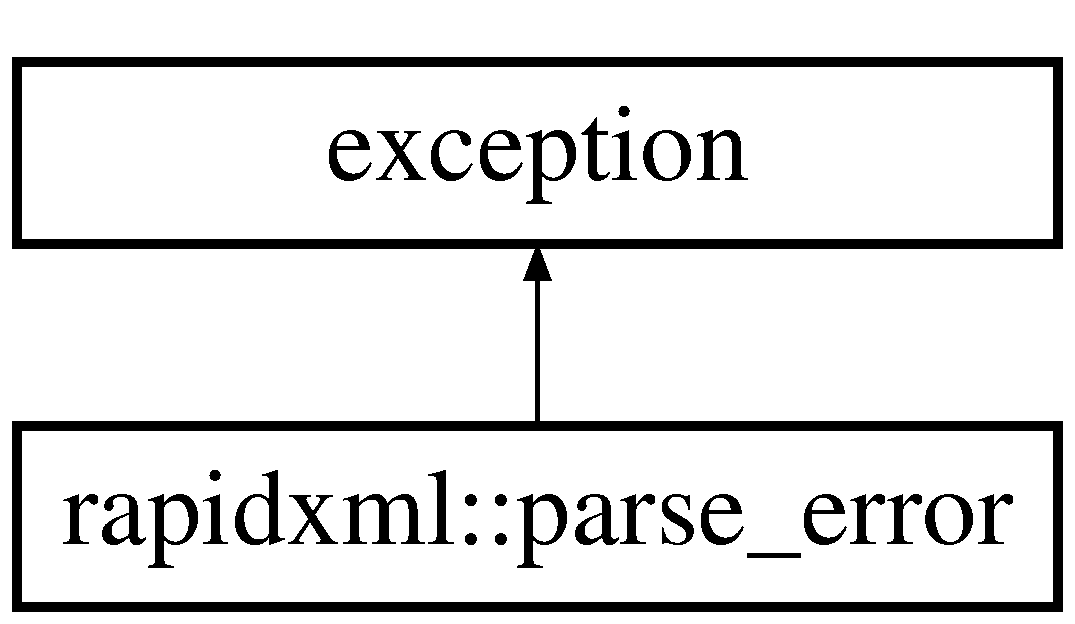
\includegraphics[height=2.000000cm]{classrapidxml_1_1parse__error}
\end{center}
\end{figure}
\subsection*{Public Member Functions}
\begin{DoxyCompactItemize}
\item 
\mbox{\Hypertarget{classrapidxml_1_1parse__error_aea12a301271c393fb627b368fb9f35c1}\label{classrapidxml_1_1parse__error_aea12a301271c393fb627b368fb9f35c1}} 
\mbox{\hyperlink{classrapidxml_1_1parse__error_aea12a301271c393fb627b368fb9f35c1}{parse\+\_\+error}} (const char $\ast$\mbox{\hyperlink{classrapidxml_1_1parse__error_a986003116ebcb49a69a20228da306232}{what}}, void $\ast$\mbox{\hyperlink{classrapidxml_1_1parse__error_ab139528f4d9e960f0ee807d22d6c032d}{where}})
\begin{DoxyCompactList}\small\item\em Constructs parse error. \end{DoxyCompactList}\item 
virtual const char $\ast$ \mbox{\hyperlink{classrapidxml_1_1parse__error_a986003116ebcb49a69a20228da306232}{what}} () const  throw ()
\item 
{\footnotesize template$<$class Ch $>$ }\\Ch $\ast$ \mbox{\hyperlink{classrapidxml_1_1parse__error_ab139528f4d9e960f0ee807d22d6c032d}{where}} () const
\end{DoxyCompactItemize}


\subsection{Detailed Description}
Parse error exception. This exception is thrown by the parser when an error occurs. Use \mbox{\hyperlink{classrapidxml_1_1parse__error_a986003116ebcb49a69a20228da306232}{what()}} function to get human-\/readable error message. Use \mbox{\hyperlink{classrapidxml_1_1parse__error_ab139528f4d9e960f0ee807d22d6c032d}{where()}} function to get a pointer to position within source text where error was detected. ~\newline
~\newline
 If throwing exceptions by the parser is undesirable, it can be disabled by defining R\+A\+P\+I\+D\+X\+M\+L\+\_\+\+N\+O\+\_\+\+E\+X\+C\+E\+P\+T\+I\+O\+NS macro before \mbox{\hyperlink{rapidxml_8hpp}{rapidxml.\+hpp}} is included. This will cause the parser to call rapidxml\+::parse\+\_\+error\+\_\+handler() function instead of throwing an exception. This function must be defined by the user. ~\newline
~\newline
 This class derives from {\ttfamily std\+::exception} class. 

\subsection{Member Function Documentation}
\mbox{\Hypertarget{classrapidxml_1_1parse__error_a986003116ebcb49a69a20228da306232}\label{classrapidxml_1_1parse__error_a986003116ebcb49a69a20228da306232}} 
\index{rapidxml\+::parse\+\_\+error@{rapidxml\+::parse\+\_\+error}!what@{what}}
\index{what@{what}!rapidxml\+::parse\+\_\+error@{rapidxml\+::parse\+\_\+error}}
\subsubsection{\texorpdfstring{what()}{what()}}
{\footnotesize\ttfamily virtual const char$\ast$ rapidxml\+::parse\+\_\+error\+::what (\begin{DoxyParamCaption}{ }\end{DoxyParamCaption}) const throw  ) \hspace{0.3cm}{\ttfamily [inline]}, {\ttfamily [virtual]}}

Gets human readable description of error. \begin{DoxyReturn}{Returns}
Pointer to null terminated description of the error. 
\end{DoxyReturn}
\mbox{\Hypertarget{classrapidxml_1_1parse__error_ab139528f4d9e960f0ee807d22d6c032d}\label{classrapidxml_1_1parse__error_ab139528f4d9e960f0ee807d22d6c032d}} 
\index{rapidxml\+::parse\+\_\+error@{rapidxml\+::parse\+\_\+error}!where@{where}}
\index{where@{where}!rapidxml\+::parse\+\_\+error@{rapidxml\+::parse\+\_\+error}}
\subsubsection{\texorpdfstring{where()}{where()}}
{\footnotesize\ttfamily template$<$class Ch $>$ \\
Ch$\ast$ rapidxml\+::parse\+\_\+error\+::where (\begin{DoxyParamCaption}{ }\end{DoxyParamCaption}) const\hspace{0.3cm}{\ttfamily [inline]}}

Gets pointer to character data where error happened. Ch should be the same as char type of \mbox{\hyperlink{classrapidxml_1_1xml__document}{xml\+\_\+document}} that produced the error. \begin{DoxyReturn}{Returns}
Pointer to location within the parsed string where error occured. 
\end{DoxyReturn}


The documentation for this class was generated from the following file\+:\begin{DoxyCompactItemize}
\item 
Tower\+Defence/\+Graphics\+Handler/\mbox{\hyperlink{rapidxml_8hpp}{rapidxml.\+hpp}}\end{DoxyCompactItemize}

\hypertarget{class_point}{}\section{Point Class Reference}
\label{class_point}\index{Point@{Point}}


Class representing logical points of the map.  




{\ttfamily \#include $<$Map.\+hpp$>$}

\subsection*{Public Types}
\begin{DoxyCompactItemize}
\item 
\mbox{\Hypertarget{class_point_a8a9b57f460ab0b37150d8de5fd7d6611}\label{class_point_a8a9b57f460ab0b37150d8de5fd7d6611}} 
enum {\bfseries Terrain\+Type} \{ {\bfseries T\+T\+\_\+\+E\+M\+P\+TY}, 
{\bfseries T\+T\+\_\+\+P\+A\+TH}, 
{\bfseries T\+T\+\_\+\+T\+O\+W\+ER}
 \}
\item 
\mbox{\Hypertarget{class_point_a308add5f0fcae4c922a72852bf9fa733}\label{class_point_a308add5f0fcae4c922a72852bf9fa733}} 
enum {\bfseries Directions} \{ {\bfseries Up}, 
{\bfseries Right}, 
{\bfseries Down}, 
{\bfseries Left}
 \}
\end{DoxyCompactItemize}
\subsection*{Public Member Functions}
\begin{DoxyCompactItemize}
\item 
\mbox{\Hypertarget{class_point_aa531683e6c851abf7e6fffdcb9fd2ad9}\label{class_point_aa531683e6c851abf7e6fffdcb9fd2ad9}} 
Directions {\bfseries operator++} (int r)
\item 
\mbox{\hyperlink{class_point_aba5766336ccc353ae31b6a0edd03bc30}{Point}} (int x=0, int y=0, int val=0)
\begin{DoxyCompactList}\small\item\em \mbox{\hyperlink{class_point}{Point}} constructor. \end{DoxyCompactList}\item 
int \mbox{\hyperlink{class_point_a1df5f9a8e3606705ebeec25384f58f8b}{GetX}} () const
\begin{DoxyCompactList}\small\item\em getter for point\textquotesingle{}s x coordinate \end{DoxyCompactList}\item 
\mbox{\Hypertarget{class_point_a28eaaae3447a8d5485a690196eb6d8da}\label{class_point_a28eaaae3447a8d5485a690196eb6d8da}} 
int \mbox{\hyperlink{class_point_a28eaaae3447a8d5485a690196eb6d8da}{GetY}} () const
\begin{DoxyCompactList}\small\item\em ~\newline
getter for point\textquotesingle{}s y coordinate \end{DoxyCompactList}\item 
Terrain\+Type \mbox{\hyperlink{class_point_af1d2f948542642bdeb25eebec21ef06f}{Get\+Terrain\+Type}} () const
\begin{DoxyCompactList}\small\item\em getter for point\textquotesingle{}s terrain type \end{DoxyCompactList}\item 
void \mbox{\hyperlink{class_point_aac7fb5fc8d1d5950f8ad7c8577ed2d65}{Set\+Terrain\+Type}} (int new\+Value)
\begin{DoxyCompactList}\small\item\em setter for point\textquotesingle{}s terrain type index \end{DoxyCompactList}\item 
void \mbox{\hyperlink{class_point_a226ab770c8f00be177167818821df9dc}{Set\+Terrain\+Type}} (Terrain\+Type new\+Value)
\begin{DoxyCompactList}\small\item\em setter for point\textquotesingle{}s terrain type \end{DoxyCompactList}\item 
bool \mbox{\hyperlink{class_point_af43939ed444048c105909fe20ec9d7a1}{Is\+Up\+Allowed}} () const
\begin{DoxyCompactList}\small\item\em checks if move in up direction is allowed \end{DoxyCompactList}\item 
bool \mbox{\hyperlink{class_point_a49b95773802999e73b390df343cc780e}{Is\+Left\+Allowed}} () const
\begin{DoxyCompactList}\small\item\em checks if move in left direction is allowed \end{DoxyCompactList}\item 
bool \mbox{\hyperlink{class_point_aa686595d33470ea204428326128aebc3}{Is\+Down\+Allowed}} () const
\begin{DoxyCompactList}\small\item\em checks if move in down direction is allowed \end{DoxyCompactList}\item 
\mbox{\Hypertarget{class_point_a0882d6fc2b88e340ecc5beb71f6930dd}\label{class_point_a0882d6fc2b88e340ecc5beb71f6930dd}} 
bool \mbox{\hyperlink{class_point_a0882d6fc2b88e340ecc5beb71f6930dd}{Is\+Right\+Allowed}} () const
\begin{DoxyCompactList}\small\item\em ~\newline
checks if move in right direction is allowed \end{DoxyCompactList}\item 
bool \mbox{\hyperlink{class_point_a30fe455d593e1f5e049bd80e374045a4}{Set\+Direction}} (bool val, Directions direction)
\begin{DoxyCompactList}\small\item\em set possibility of move in chosen direction \end{DoxyCompactList}\item 
bool \mbox{\hyperlink{class_point_ae8e3d753aeaa848e2cc27d1a95f31646}{Allow\+Up}} ()
\begin{DoxyCompactList}\small\item\em set possibility of move in up direction \end{DoxyCompactList}\item 
\mbox{\Hypertarget{class_point_a1f334c775c9b49f3bfe9591dc267eb59}\label{class_point_a1f334c775c9b49f3bfe9591dc267eb59}} 
bool \mbox{\hyperlink{class_point_a1f334c775c9b49f3bfe9591dc267eb59}{Allow\+Down}} ()
\begin{DoxyCompactList}\small\item\em ~\newline
set possibility of move in down direction \end{DoxyCompactList}\item 
bool \mbox{\hyperlink{class_point_a29eb3406055020f0e40bdf130ea74ee0}{Allow\+Left}} ()
\begin{DoxyCompactList}\small\item\em set possibility of move in left direction \end{DoxyCompactList}\item 
bool \mbox{\hyperlink{class_point_a92545dd0cf053357f70f809bf32a759f}{Allow\+Right}} ()
\begin{DoxyCompactList}\small\item\em set possibility of move in right direction \end{DoxyCompactList}\item 
bool \mbox{\hyperlink{class_point_a61ee1b109f1edf11cfa37b16e9113e9f}{Disallow\+Up}} ()
\begin{DoxyCompactList}\small\item\em makes move in up direction impossible \end{DoxyCompactList}\item 
bool \mbox{\hyperlink{class_point_ab1d92678fc5ba39f65649144a261d6f4}{Disallow\+Down}} ()
\begin{DoxyCompactList}\small\item\em makes move in down direction impossible \end{DoxyCompactList}\item 
bool \mbox{\hyperlink{class_point_a9a3dacc41ce29ba4535b99e9d0c6575e}{Disallow\+Left}} ()
\begin{DoxyCompactList}\small\item\em makes move in left direction impossible \end{DoxyCompactList}\item 
bool \mbox{\hyperlink{class_point_a38a55e9eae750c1e3838c1572b1b8ae2}{Disallow\+Right}} ()
\begin{DoxyCompactList}\small\item\em makes move in right direction impossible \end{DoxyCompactList}\item 
\mbox{\hyperlink{class_point}{Point}} \mbox{\hyperlink{class_point_ad6451227b0442af26b62280f7fe33eac}{Get\+Next}} () const
\begin{DoxyCompactList}\small\item\em Get next point. \end{DoxyCompactList}\item 
bool \mbox{\hyperlink{class_point_a7cda0356e8cf4ca2daae36fe45273d77}{operator==}} (const \mbox{\hyperlink{class_point}{Point}} \&rhv) const
\begin{DoxyCompactList}\small\item\em overloaded comparison operator \end{DoxyCompactList}\end{DoxyCompactItemize}


\subsection{Detailed Description}
Class representing logical points of the map. 

\subsection{Constructor \& Destructor Documentation}
\mbox{\Hypertarget{class_point_aba5766336ccc353ae31b6a0edd03bc30}\label{class_point_aba5766336ccc353ae31b6a0edd03bc30}} 
\index{Point@{Point}!Point@{Point}}
\index{Point@{Point}!Point@{Point}}
\subsubsection{\texorpdfstring{Point()}{Point()}}
{\footnotesize\ttfamily Point\+::\+Point (\begin{DoxyParamCaption}\item[{int}]{x = {\ttfamily 0},  }\item[{int}]{y = {\ttfamily 0},  }\item[{int}]{val = {\ttfamily 0} }\end{DoxyParamCaption})\hspace{0.3cm}{\ttfamily [explicit]}}



\mbox{\hyperlink{class_point}{Point}} constructor. 


\begin{DoxyParams}{Parameters}
{\em x} & \\
\hline
{\em y} & \\
\hline
{\em value} & \\
\hline
\end{DoxyParams}


\subsection{Member Function Documentation}
\mbox{\Hypertarget{class_point_a29eb3406055020f0e40bdf130ea74ee0}\label{class_point_a29eb3406055020f0e40bdf130ea74ee0}} 
\index{Point@{Point}!Allow\+Left@{Allow\+Left}}
\index{Allow\+Left@{Allow\+Left}!Point@{Point}}
\subsubsection{\texorpdfstring{Allow\+Left()}{AllowLeft()}}
{\footnotesize\ttfamily bool Point\+::\+Allow\+Left (\begin{DoxyParamCaption}{ }\end{DoxyParamCaption})}



set possibility of move in left direction 

\begin{DoxyReturn}{Returns}
logical whether move in left direction was allowed 
\end{DoxyReturn}
\mbox{\Hypertarget{class_point_a92545dd0cf053357f70f809bf32a759f}\label{class_point_a92545dd0cf053357f70f809bf32a759f}} 
\index{Point@{Point}!Allow\+Right@{Allow\+Right}}
\index{Allow\+Right@{Allow\+Right}!Point@{Point}}
\subsubsection{\texorpdfstring{Allow\+Right()}{AllowRight()}}
{\footnotesize\ttfamily bool Point\+::\+Allow\+Right (\begin{DoxyParamCaption}{ }\end{DoxyParamCaption})}



set possibility of move in right direction 

\begin{DoxyReturn}{Returns}
logical whether move in right direction was allowed 
\end{DoxyReturn}
\mbox{\Hypertarget{class_point_ae8e3d753aeaa848e2cc27d1a95f31646}\label{class_point_ae8e3d753aeaa848e2cc27d1a95f31646}} 
\index{Point@{Point}!Allow\+Up@{Allow\+Up}}
\index{Allow\+Up@{Allow\+Up}!Point@{Point}}
\subsubsection{\texorpdfstring{Allow\+Up()}{AllowUp()}}
{\footnotesize\ttfamily bool Point\+::\+Allow\+Up (\begin{DoxyParamCaption}{ }\end{DoxyParamCaption})}



set possibility of move in up direction 

\begin{DoxyReturn}{Returns}
logical whether move in up direction was allowed 
\end{DoxyReturn}
\mbox{\Hypertarget{class_point_ab1d92678fc5ba39f65649144a261d6f4}\label{class_point_ab1d92678fc5ba39f65649144a261d6f4}} 
\index{Point@{Point}!Disallow\+Down@{Disallow\+Down}}
\index{Disallow\+Down@{Disallow\+Down}!Point@{Point}}
\subsubsection{\texorpdfstring{Disallow\+Down()}{DisallowDown()}}
{\footnotesize\ttfamily bool Point\+::\+Disallow\+Down (\begin{DoxyParamCaption}{ }\end{DoxyParamCaption})}



makes move in down direction impossible 

\begin{DoxyReturn}{Returns}
logical whether move in down direction wasn\textquotesingle{}t allowed 
\end{DoxyReturn}
\mbox{\Hypertarget{class_point_a9a3dacc41ce29ba4535b99e9d0c6575e}\label{class_point_a9a3dacc41ce29ba4535b99e9d0c6575e}} 
\index{Point@{Point}!Disallow\+Left@{Disallow\+Left}}
\index{Disallow\+Left@{Disallow\+Left}!Point@{Point}}
\subsubsection{\texorpdfstring{Disallow\+Left()}{DisallowLeft()}}
{\footnotesize\ttfamily bool Point\+::\+Disallow\+Left (\begin{DoxyParamCaption}{ }\end{DoxyParamCaption})}



makes move in left direction impossible 

\begin{DoxyReturn}{Returns}
logical whether move in left direction wasn\textquotesingle{}t allowed 
\end{DoxyReturn}
\mbox{\Hypertarget{class_point_a38a55e9eae750c1e3838c1572b1b8ae2}\label{class_point_a38a55e9eae750c1e3838c1572b1b8ae2}} 
\index{Point@{Point}!Disallow\+Right@{Disallow\+Right}}
\index{Disallow\+Right@{Disallow\+Right}!Point@{Point}}
\subsubsection{\texorpdfstring{Disallow\+Right()}{DisallowRight()}}
{\footnotesize\ttfamily bool Point\+::\+Disallow\+Right (\begin{DoxyParamCaption}{ }\end{DoxyParamCaption})}



makes move in right direction impossible 

\begin{DoxyReturn}{Returns}
logical whether move in right direction wasn\textquotesingle{}t allowed 
\end{DoxyReturn}
\mbox{\Hypertarget{class_point_a61ee1b109f1edf11cfa37b16e9113e9f}\label{class_point_a61ee1b109f1edf11cfa37b16e9113e9f}} 
\index{Point@{Point}!Disallow\+Up@{Disallow\+Up}}
\index{Disallow\+Up@{Disallow\+Up}!Point@{Point}}
\subsubsection{\texorpdfstring{Disallow\+Up()}{DisallowUp()}}
{\footnotesize\ttfamily bool Point\+::\+Disallow\+Up (\begin{DoxyParamCaption}{ }\end{DoxyParamCaption})}



makes move in up direction impossible 

\begin{DoxyReturn}{Returns}
logical whether move in up direction wasn\textquotesingle{}t allowed 
\end{DoxyReturn}
\mbox{\Hypertarget{class_point_ad6451227b0442af26b62280f7fe33eac}\label{class_point_ad6451227b0442af26b62280f7fe33eac}} 
\index{Point@{Point}!Get\+Next@{Get\+Next}}
\index{Get\+Next@{Get\+Next}!Point@{Point}}
\subsubsection{\texorpdfstring{Get\+Next()}{GetNext()}}
{\footnotesize\ttfamily \mbox{\hyperlink{class_point}{Point}} Point\+::\+Get\+Next (\begin{DoxyParamCaption}{ }\end{DoxyParamCaption}) const}



Get next point. 

\begin{DoxyReturn}{Returns}
point with specific coordinates and value 
\end{DoxyReturn}
\mbox{\Hypertarget{class_point_af1d2f948542642bdeb25eebec21ef06f}\label{class_point_af1d2f948542642bdeb25eebec21ef06f}} 
\index{Point@{Point}!Get\+Terrain\+Type@{Get\+Terrain\+Type}}
\index{Get\+Terrain\+Type@{Get\+Terrain\+Type}!Point@{Point}}
\subsubsection{\texorpdfstring{Get\+Terrain\+Type()}{GetTerrainType()}}
{\footnotesize\ttfamily Point\+::\+Terrain\+Type Point\+::\+Get\+Terrain\+Type (\begin{DoxyParamCaption}{ }\end{DoxyParamCaption}) const}



getter for point\textquotesingle{}s terrain type 

\begin{DoxyReturn}{Returns}
terrain type 
\end{DoxyReturn}
\mbox{\Hypertarget{class_point_a1df5f9a8e3606705ebeec25384f58f8b}\label{class_point_a1df5f9a8e3606705ebeec25384f58f8b}} 
\index{Point@{Point}!GetX@{GetX}}
\index{GetX@{GetX}!Point@{Point}}
\subsubsection{\texorpdfstring{Get\+X()}{GetX()}}
{\footnotesize\ttfamily int Point\+::\+GetX (\begin{DoxyParamCaption}{ }\end{DoxyParamCaption}) const}



getter for point\textquotesingle{}s x coordinate 

\begin{DoxyReturn}{Returns}
x value 
\end{DoxyReturn}
\mbox{\Hypertarget{class_point_aa686595d33470ea204428326128aebc3}\label{class_point_aa686595d33470ea204428326128aebc3}} 
\index{Point@{Point}!Is\+Down\+Allowed@{Is\+Down\+Allowed}}
\index{Is\+Down\+Allowed@{Is\+Down\+Allowed}!Point@{Point}}
\subsubsection{\texorpdfstring{Is\+Down\+Allowed()}{IsDownAllowed()}}
{\footnotesize\ttfamily bool Point\+::\+Is\+Down\+Allowed (\begin{DoxyParamCaption}{ }\end{DoxyParamCaption}) const}



checks if move in down direction is allowed 

\begin{DoxyReturn}{Returns}
logical indicating whether move in down direction is allowed 
\end{DoxyReturn}
\mbox{\Hypertarget{class_point_a49b95773802999e73b390df343cc780e}\label{class_point_a49b95773802999e73b390df343cc780e}} 
\index{Point@{Point}!Is\+Left\+Allowed@{Is\+Left\+Allowed}}
\index{Is\+Left\+Allowed@{Is\+Left\+Allowed}!Point@{Point}}
\subsubsection{\texorpdfstring{Is\+Left\+Allowed()}{IsLeftAllowed()}}
{\footnotesize\ttfamily bool Point\+::\+Is\+Left\+Allowed (\begin{DoxyParamCaption}{ }\end{DoxyParamCaption}) const}



checks if move in left direction is allowed 

\begin{DoxyReturn}{Returns}
logical indicating whether move in left direction is allowed 
\end{DoxyReturn}
\mbox{\Hypertarget{class_point_af43939ed444048c105909fe20ec9d7a1}\label{class_point_af43939ed444048c105909fe20ec9d7a1}} 
\index{Point@{Point}!Is\+Up\+Allowed@{Is\+Up\+Allowed}}
\index{Is\+Up\+Allowed@{Is\+Up\+Allowed}!Point@{Point}}
\subsubsection{\texorpdfstring{Is\+Up\+Allowed()}{IsUpAllowed()}}
{\footnotesize\ttfamily bool Point\+::\+Is\+Up\+Allowed (\begin{DoxyParamCaption}{ }\end{DoxyParamCaption}) const}



checks if move in up direction is allowed 

\begin{DoxyReturn}{Returns}
logical indicating whether move in up direction is allowed 
\end{DoxyReturn}
\mbox{\Hypertarget{class_point_a7cda0356e8cf4ca2daae36fe45273d77}\label{class_point_a7cda0356e8cf4ca2daae36fe45273d77}} 
\index{Point@{Point}!operator==@{operator==}}
\index{operator==@{operator==}!Point@{Point}}
\subsubsection{\texorpdfstring{operator==()}{operator==()}}
{\footnotesize\ttfamily bool Point\+::operator== (\begin{DoxyParamCaption}\item[{const \mbox{\hyperlink{class_point}{Point}} \&}]{rhv }\end{DoxyParamCaption}) const}



overloaded comparison operator 

\begin{DoxyReturn}{Returns}
logical indicating whether two points coordinates are equal 
\end{DoxyReturn}
\mbox{\Hypertarget{class_point_a30fe455d593e1f5e049bd80e374045a4}\label{class_point_a30fe455d593e1f5e049bd80e374045a4}} 
\index{Point@{Point}!Set\+Direction@{Set\+Direction}}
\index{Set\+Direction@{Set\+Direction}!Point@{Point}}
\subsubsection{\texorpdfstring{Set\+Direction()}{SetDirection()}}
{\footnotesize\ttfamily bool Point\+::\+Set\+Direction (\begin{DoxyParamCaption}\item[{bool}]{val,  }\item[{Directions}]{direction }\end{DoxyParamCaption})}



set possibility of move in chosen direction 

\begin{DoxyReturn}{Returns}
logical whether move in chosen direction is allowed 
\end{DoxyReturn}
\mbox{\Hypertarget{class_point_aac7fb5fc8d1d5950f8ad7c8577ed2d65}\label{class_point_aac7fb5fc8d1d5950f8ad7c8577ed2d65}} 
\index{Point@{Point}!Set\+Terrain\+Type@{Set\+Terrain\+Type}}
\index{Set\+Terrain\+Type@{Set\+Terrain\+Type}!Point@{Point}}
\subsubsection{\texorpdfstring{Set\+Terrain\+Type()}{SetTerrainType()}\hspace{0.1cm}{\footnotesize\ttfamily [1/2]}}
{\footnotesize\ttfamily void Point\+::\+Set\+Terrain\+Type (\begin{DoxyParamCaption}\item[{int}]{new\+Value }\end{DoxyParamCaption})}



setter for point\textquotesingle{}s terrain type index 


\begin{DoxyParams}{Parameters}
{\em terrain} & type number \\
\hline
\end{DoxyParams}
\mbox{\Hypertarget{class_point_a226ab770c8f00be177167818821df9dc}\label{class_point_a226ab770c8f00be177167818821df9dc}} 
\index{Point@{Point}!Set\+Terrain\+Type@{Set\+Terrain\+Type}}
\index{Set\+Terrain\+Type@{Set\+Terrain\+Type}!Point@{Point}}
\subsubsection{\texorpdfstring{Set\+Terrain\+Type()}{SetTerrainType()}\hspace{0.1cm}{\footnotesize\ttfamily [2/2]}}
{\footnotesize\ttfamily void Point\+::\+Set\+Terrain\+Type (\begin{DoxyParamCaption}\item[{Terrain\+Type}]{new\+Value }\end{DoxyParamCaption})}



setter for point\textquotesingle{}s terrain type 


\begin{DoxyParams}{Parameters}
{\em terrain} & type \\
\hline
\end{DoxyParams}


The documentation for this class was generated from the following files\+:\begin{DoxyCompactItemize}
\item 
Tower\+Defence/\+Graphics\+Handler/Map.\+hpp\item 
Tower\+Defence/\+Graphics\+Handler/Map.\+cpp\end{DoxyCompactItemize}

\hypertarget{class_rules_file_parser}{}\section{Rules\+File\+Parser Class Reference}
\label{class_rules_file_parser}\index{Rules\+File\+Parser@{Rules\+File\+Parser}}


Class used for parsing file containing rule\textquotesingle{}s settings.  




{\ttfamily \#include $<$Map.\+hpp$>$}



\subsection{Detailed Description}
Class used for parsing file containing rule\textquotesingle{}s settings. 

The documentation for this class was generated from the following file\+:\begin{DoxyCompactItemize}
\item 
Tower\+Defence/\+Graphics\+Handler/Map.\+hpp\end{DoxyCompactItemize}

\hypertarget{class_scene}{}\section{Scene Class Reference}
\label{class_scene}\index{Scene@{Scene}}


Class representing game scene.  




{\ttfamily \#include $<$Scene.\+h$>$}

Inheritance diagram for Scene\+:\begin{figure}[H]
\begin{center}
\leavevmode
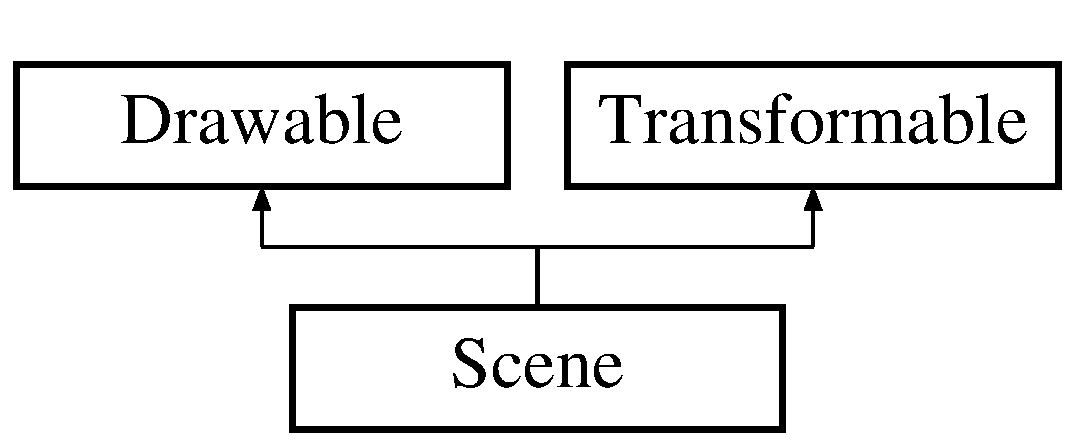
\includegraphics[height=2.000000cm]{class_scene}
\end{center}
\end{figure}
\subsection*{Public Member Functions}
\begin{DoxyCompactItemize}
\item 
\mbox{\hyperlink{class_scene_a7a4f0004dce8380ca0e31f573a92d7f2}{Scene}} (\mbox{\hyperlink{class_map}{Map}} map)
\begin{DoxyCompactList}\small\item\em Constructor, creates scene based on delivered map. \end{DoxyCompactList}\item 
\mbox{\Hypertarget{class_scene_ae1b864ad69216f68b5c588477c87ec20}\label{class_scene_ae1b864ad69216f68b5c588477c87ec20}} 
void \mbox{\hyperlink{class_scene_ae1b864ad69216f68b5c588477c87ec20}{load}} ()
\begin{DoxyCompactList}\small\item\em Prepares array of verticles according to logical map. \end{DoxyCompactList}\item 
\mbox{\Hypertarget{class_scene_a3b8cec2e32546713915f8c6303c951f1}\label{class_scene_a3b8cec2e32546713915f8c6303c951f1}} 
virtual \mbox{\hyperlink{class_scene_a3b8cec2e32546713915f8c6303c951f1}{$\sim$\+Scene}} ()
\begin{DoxyCompactList}\small\item\em Destructor. \end{DoxyCompactList}\item 
void \mbox{\hyperlink{class_scene_a77d8f570a3b13a237b31888429288946}{Push\+Object}} (\mbox{\hyperlink{class_i_moveable}{I\+Moveable}} $\ast$obj)
\begin{DoxyCompactList}\small\item\em Adds moveable object to collection. \end{DoxyCompactList}\item 
sf\+::\+Vector2f \mbox{\hyperlink{class_scene_a527feb6bbb5f751494fac5a3503657e7}{get\+Square\+Origin}} (\mbox{\hyperlink{class_point}{Point}} p) const
\begin{DoxyCompactList}\small\item\em Gets center of square corresponding to a particular point. \end{DoxyCompactList}\item 
const \mbox{\hyperlink{class_map}{Map}} \& \mbox{\hyperlink{class_scene_a63e098d10e04e864474e4949690c6f57}{get\+Map}} () const
\begin{DoxyCompactList}\small\item\em Gets object of logical map. \end{DoxyCompactList}\item 
\mbox{\Hypertarget{class_scene_aa3add49578abdf4d3fd3fb47192d6e8e}\label{class_scene_aa3add49578abdf4d3fd3fb47192d6e8e}} 
void \mbox{\hyperlink{class_scene_aa3add49578abdf4d3fd3fb47192d6e8e}{Cleanup}} ()
\begin{DoxyCompactList}\small\item\em Removes outdated moveable objects from scene. \end{DoxyCompactList}\item 
void \mbox{\hyperlink{class_scene_a0cd0a324b6fd0d560ce223e249be0828}{Update\+Scene}} ()
\begin{DoxyCompactList}\small\item\em Updates object on the scene. \end{DoxyCompactList}\item 
void \mbox{\hyperlink{class_scene_a9c715dfd2169aa537526947c6649b397}{set\+Towers}} (\mbox{\hyperlink{class_tower_manager}{Tower\+Manager}} $\ast$tower)
\begin{DoxyCompactList}\small\item\em Sets and loads object managing towers. \end{DoxyCompactList}\item 
Moveable\+Vector \mbox{\hyperlink{class_scene_a0e995515914c7ac027c8814f3bd341da}{Get\+Moveable\+Objects}} ()
\begin{DoxyCompactList}\small\item\em Gets collection of moveable obiects. \end{DoxyCompactList}\item 
bool \mbox{\hyperlink{class_scene_ad868aeb65543a3bd92b722b976885549}{End\+Of\+Wave}} ()
\begin{DoxyCompactList}\small\item\em Check if there are any enemies or bullets on the scene. \end{DoxyCompactList}\item 
int \mbox{\hyperlink{class_scene_a59c3ff8674ae5156614afe53d2797337}{Enemy\+At\+End}} ()
\begin{DoxyCompactList}\small\item\em Check if there are enemies at the end of path. \end{DoxyCompactList}\end{DoxyCompactItemize}


\subsection{Detailed Description}
Class representing game scene. 

Contains all graphical elements of game, such as graphical representation of map and collections of towers, enemies, etc. ~\newline
Object of this type is the main rendered object in game 

\subsection{Constructor \& Destructor Documentation}
\mbox{\Hypertarget{class_scene_a7a4f0004dce8380ca0e31f573a92d7f2}\label{class_scene_a7a4f0004dce8380ca0e31f573a92d7f2}} 
\index{Scene@{Scene}!Scene@{Scene}}
\index{Scene@{Scene}!Scene@{Scene}}
\subsubsection{\texorpdfstring{Scene()}{Scene()}}
{\footnotesize\ttfamily Scene\+::\+Scene (\begin{DoxyParamCaption}\item[{\mbox{\hyperlink{class_map}{Map}}}]{map }\end{DoxyParamCaption})}



Constructor, creates scene based on delivered map. 


\begin{DoxyParams}{Parameters}
{\em map} & logical map \\
\hline
\end{DoxyParams}


\subsection{Member Function Documentation}
\mbox{\Hypertarget{class_scene_ad868aeb65543a3bd92b722b976885549}\label{class_scene_ad868aeb65543a3bd92b722b976885549}} 
\index{Scene@{Scene}!End\+Of\+Wave@{End\+Of\+Wave}}
\index{End\+Of\+Wave@{End\+Of\+Wave}!Scene@{Scene}}
\subsubsection{\texorpdfstring{End\+Of\+Wave()}{EndOfWave()}}
{\footnotesize\ttfamily bool Scene\+::\+End\+Of\+Wave (\begin{DoxyParamCaption}{ }\end{DoxyParamCaption})}



Check if there are any enemies or bullets on the scene. 

\begin{DoxyReturn}{Returns}
true if wave still lasts, false otherwise 
\end{DoxyReturn}
\mbox{\Hypertarget{class_scene_a59c3ff8674ae5156614afe53d2797337}\label{class_scene_a59c3ff8674ae5156614afe53d2797337}} 
\index{Scene@{Scene}!Enemy\+At\+End@{Enemy\+At\+End}}
\index{Enemy\+At\+End@{Enemy\+At\+End}!Scene@{Scene}}
\subsubsection{\texorpdfstring{Enemy\+At\+End()}{EnemyAtEnd()}}
{\footnotesize\ttfamily int Scene\+::\+Enemy\+At\+End (\begin{DoxyParamCaption}{ }\end{DoxyParamCaption})}



Check if there are enemies at the end of path. 

All enemies that have achieved end of the path are killed and total damage is computed \begin{DoxyReturn}{Returns}
total damage done by the enemies 
\end{DoxyReturn}
\mbox{\Hypertarget{class_scene_a63e098d10e04e864474e4949690c6f57}\label{class_scene_a63e098d10e04e864474e4949690c6f57}} 
\index{Scene@{Scene}!get\+Map@{get\+Map}}
\index{get\+Map@{get\+Map}!Scene@{Scene}}
\subsubsection{\texorpdfstring{get\+Map()}{getMap()}}
{\footnotesize\ttfamily const \mbox{\hyperlink{class_map}{Map}} \& Scene\+::get\+Map (\begin{DoxyParamCaption}{ }\end{DoxyParamCaption}) const}



Gets object of logical map. 

\begin{DoxyReturn}{Returns}
map 
\end{DoxyReturn}
\mbox{\Hypertarget{class_scene_a0e995515914c7ac027c8814f3bd341da}\label{class_scene_a0e995515914c7ac027c8814f3bd341da}} 
\index{Scene@{Scene}!Get\+Moveable\+Objects@{Get\+Moveable\+Objects}}
\index{Get\+Moveable\+Objects@{Get\+Moveable\+Objects}!Scene@{Scene}}
\subsubsection{\texorpdfstring{Get\+Moveable\+Objects()}{GetMoveableObjects()}}
{\footnotesize\ttfamily Moveable\+Vector Scene\+::\+Get\+Moveable\+Objects (\begin{DoxyParamCaption}{ }\end{DoxyParamCaption})}



Gets collection of moveable obiects. 

\begin{DoxyReturn}{Returns}
vector of moveable obiects 
\end{DoxyReturn}
\mbox{\Hypertarget{class_scene_a527feb6bbb5f751494fac5a3503657e7}\label{class_scene_a527feb6bbb5f751494fac5a3503657e7}} 
\index{Scene@{Scene}!get\+Square\+Origin@{get\+Square\+Origin}}
\index{get\+Square\+Origin@{get\+Square\+Origin}!Scene@{Scene}}
\subsubsection{\texorpdfstring{get\+Square\+Origin()}{getSquareOrigin()}}
{\footnotesize\ttfamily sf\+::\+Vector2f Scene\+::get\+Square\+Origin (\begin{DoxyParamCaption}\item[{\mbox{\hyperlink{class_point}{Point}}}]{p }\end{DoxyParamCaption}) const}



Gets center of square corresponding to a particular point. 


\begin{DoxyParams}{Parameters}
{\em p} & point describing a square \\
\hline
\end{DoxyParams}
\begin{DoxyReturn}{Returns}
center of indicated square 
\end{DoxyReturn}
\mbox{\Hypertarget{class_scene_a77d8f570a3b13a237b31888429288946}\label{class_scene_a77d8f570a3b13a237b31888429288946}} 
\index{Scene@{Scene}!Push\+Object@{Push\+Object}}
\index{Push\+Object@{Push\+Object}!Scene@{Scene}}
\subsubsection{\texorpdfstring{Push\+Object()}{PushObject()}}
{\footnotesize\ttfamily void Scene\+::\+Push\+Object (\begin{DoxyParamCaption}\item[{\mbox{\hyperlink{class_i_moveable}{I\+Moveable}} $\ast$}]{obj }\end{DoxyParamCaption})}



Adds moveable object to collection. 


\begin{DoxyParams}{Parameters}
{\em obj} & pointer to moveable object \\
\hline
\end{DoxyParams}
\mbox{\Hypertarget{class_scene_a9c715dfd2169aa537526947c6649b397}\label{class_scene_a9c715dfd2169aa537526947c6649b397}} 
\index{Scene@{Scene}!set\+Towers@{set\+Towers}}
\index{set\+Towers@{set\+Towers}!Scene@{Scene}}
\subsubsection{\texorpdfstring{set\+Towers()}{setTowers()}}
{\footnotesize\ttfamily void Scene\+::set\+Towers (\begin{DoxyParamCaption}\item[{\mbox{\hyperlink{class_tower_manager}{Tower\+Manager}} $\ast$}]{tower }\end{DoxyParamCaption})}



Sets and loads object managing towers. 


\begin{DoxyParams}{Parameters}
{\em tower} & pointer to new \mbox{\hyperlink{class_tower_manager}{Tower\+Manager}} object \\
\hline
\end{DoxyParams}
\mbox{\Hypertarget{class_scene_a0cd0a324b6fd0d560ce223e249be0828}\label{class_scene_a0cd0a324b6fd0d560ce223e249be0828}} 
\index{Scene@{Scene}!Update\+Scene@{Update\+Scene}}
\index{Update\+Scene@{Update\+Scene}!Scene@{Scene}}
\subsubsection{\texorpdfstring{Update\+Scene()}{UpdateScene()}}
{\footnotesize\ttfamily void Scene\+::\+Update\+Scene (\begin{DoxyParamCaption}{ }\end{DoxyParamCaption})}



Updates object on the scene. 

Adds new objects to scene, moves objects, checks collisions and removes inactive objects 

The documentation for this class was generated from the following files\+:\begin{DoxyCompactItemize}
\item 
Tower\+Defence/\+Graphics\+Handler/Scene.\+h\item 
Tower\+Defence/\+Graphics\+Handler/Scene.\+cpp\end{DoxyCompactItemize}

\hypertarget{class_snake}{}\section{Snake Class Reference}
\label{class_snake}\index{Snake@{Snake}}


Class representing snake.  




{\ttfamily \#include $<$Enemy\+Designer.\+h$>$}

Inheritance diagram for Snake\+:\begin{figure}[H]
\begin{center}
\leavevmode
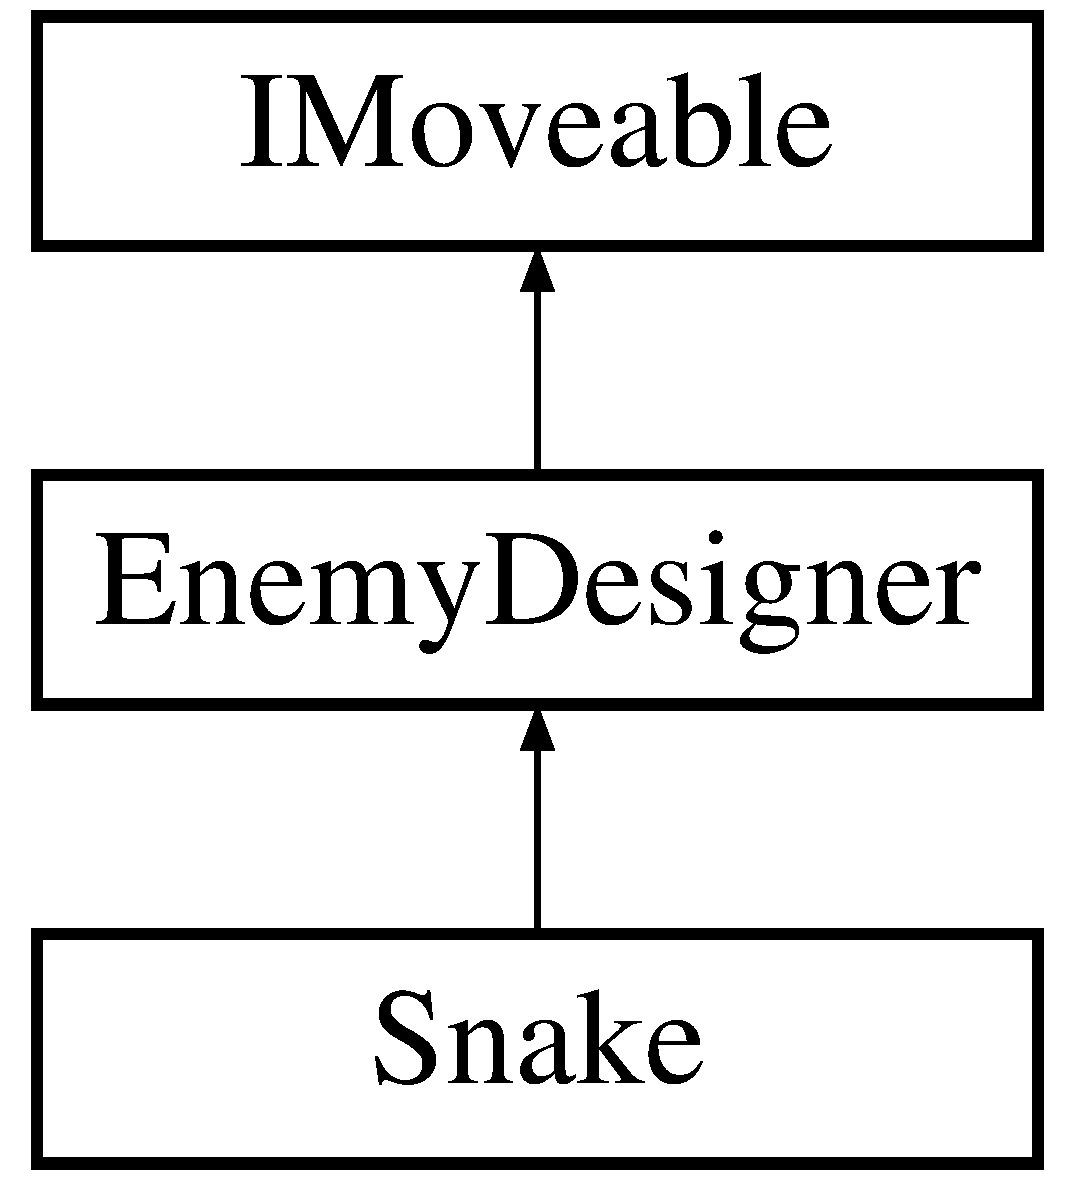
\includegraphics[height=3.000000cm]{class_snake}
\end{center}
\end{figure}
\subsection*{Public Member Functions}
\begin{DoxyCompactItemize}
\item 
\mbox{\hyperlink{class_snake_a92f93daaa158c71469ee4ba468922442}{Snake}} (sf\+::\+Vector2f origin, sf\+::\+Vector2f dimensions, sf\+::\+Color color, sf\+::\+Vector2f texture\+Dimensions, std\+::string texture\+File=\char`\"{}set\+Of\+Monsters.\+png\char`\"{})
\begin{DoxyCompactList}\small\item\em constructor for snake class \end{DoxyCompactList}\end{DoxyCompactItemize}
\subsection*{Additional Inherited Members}


\subsection{Detailed Description}
Class representing snake. 

\subsection{Constructor \& Destructor Documentation}
\mbox{\Hypertarget{class_snake_a92f93daaa158c71469ee4ba468922442}\label{class_snake_a92f93daaa158c71469ee4ba468922442}} 
\index{Snake@{Snake}!Snake@{Snake}}
\index{Snake@{Snake}!Snake@{Snake}}
\subsubsection{\texorpdfstring{Snake()}{Snake()}}
{\footnotesize\ttfamily Snake\+::\+Snake (\begin{DoxyParamCaption}\item[{sf\+::\+Vector2f}]{origin,  }\item[{sf\+::\+Vector2f}]{dimensions,  }\item[{sf\+::\+Color}]{color,  }\item[{sf\+::\+Vector2f}]{texture\+Dimensions,  }\item[{std\+::string}]{texture\+File = {\ttfamily \char`\"{}setOfMonsters.png\char`\"{}} }\end{DoxyParamCaption})}



constructor for snake class 


\begin{DoxyParams}{Parameters}
{\em origin} & point \\
\hline
{\em dimensions} & \\
\hline
{\em color} & \\
\hline
{\em texture} & dimensions \\
\hline
{\em file} & containing texture \\
\hline
\end{DoxyParams}


The documentation for this class was generated from the following files\+:\begin{DoxyCompactItemize}
\item 
Tower\+Defence/\+Graphics\+Handler/Enemy\+Designer.\+h\item 
Tower\+Defence/\+Graphics\+Handler/Enemy\+Designer.\+cpp\end{DoxyCompactItemize}

\hypertarget{class_statistics}{}\section{Statistics Class Reference}
\label{class_statistics}\index{Statistics@{Statistics}}


Class representing monster\textquotesingle{}s statistics.  




{\ttfamily \#include $<$Enemy\+Base.\+hpp$>$}

\subsection*{Public Member Functions}
\begin{DoxyCompactItemize}
\item 
\mbox{\hyperlink{class_statistics_a66445b3151e74a15b543437eb2633a72}{Statistics}} (uint health=0, uint damage=0, uint speed=0)
\begin{DoxyCompactList}\small\item\em statistics constructor \end{DoxyCompactList}\item 
\mbox{\Hypertarget{class_statistics_a0a1a2e5163182a42349449a0a44145fb}\label{class_statistics_a0a1a2e5163182a42349449a0a44145fb}} 
int \mbox{\hyperlink{class_statistics_a0a1a2e5163182a42349449a0a44145fb}{Get\+Health}} ()
\begin{DoxyCompactList}\small\item\em getter for health \end{DoxyCompactList}\item 
void \mbox{\hyperlink{class_statistics_a152114e1a7134507f3f1865f05ae6ac9}{Set\+Health}} (uint health)
\begin{DoxyCompactList}\small\item\em setter for health \end{DoxyCompactList}\item 
int \mbox{\hyperlink{class_statistics_a46693e6826f75d2b1b40c1ea34707096}{Get\+Damage}} ()
\begin{DoxyCompactList}\small\item\em getter for damage \end{DoxyCompactList}\item 
int \mbox{\hyperlink{class_statistics_a055c86f402070457d85468dc9c8e0b5a}{Get\+Speed}} ()
\begin{DoxyCompactList}\small\item\em getter for speed \end{DoxyCompactList}\item 
int \mbox{\hyperlink{class_statistics_a5f6ba53f54849e07de0e30ae7b07e818}{Get\+Value}} ()
\begin{DoxyCompactList}\small\item\em getter for value of the enemy \end{DoxyCompactList}\item 
\mbox{\Hypertarget{class_statistics_ab68ede75479e44d5c35b78ec1284065b}\label{class_statistics_ab68ede75479e44d5c35b78ec1284065b}} 
\mbox{\hyperlink{class_statistics_ab68ede75479e44d5c35b78ec1284065b}{$\sim$\+Statistics}} ()
\begin{DoxyCompactList}\small\item\em destructor \end{DoxyCompactList}\end{DoxyCompactItemize}


\subsection{Detailed Description}
Class representing monster\textquotesingle{}s statistics. 

\subsection{Constructor \& Destructor Documentation}
\mbox{\Hypertarget{class_statistics_a66445b3151e74a15b543437eb2633a72}\label{class_statistics_a66445b3151e74a15b543437eb2633a72}} 
\index{Statistics@{Statistics}!Statistics@{Statistics}}
\index{Statistics@{Statistics}!Statistics@{Statistics}}
\subsubsection{\texorpdfstring{Statistics()}{Statistics()}}
{\footnotesize\ttfamily Statistics\+::\+Statistics (\begin{DoxyParamCaption}\item[{uint}]{health = {\ttfamily 0},  }\item[{uint}]{damage = {\ttfamily 0},  }\item[{uint}]{speed = {\ttfamily 0} }\end{DoxyParamCaption})\hspace{0.3cm}{\ttfamily [explicit]}}



statistics constructor 


\begin{DoxyParams}{Parameters}
{\em enemy\textquotesingle{}s} & health \\
\hline
{\em enemy\textquotesingle{}s} & damage \\
\hline
{\em enemy\textquotesingle{}s} & speed \\
\hline
\end{DoxyParams}


\subsection{Member Function Documentation}
\mbox{\Hypertarget{class_statistics_a46693e6826f75d2b1b40c1ea34707096}\label{class_statistics_a46693e6826f75d2b1b40c1ea34707096}} 
\index{Statistics@{Statistics}!Get\+Damage@{Get\+Damage}}
\index{Get\+Damage@{Get\+Damage}!Statistics@{Statistics}}
\subsubsection{\texorpdfstring{Get\+Damage()}{GetDamage()}}
{\footnotesize\ttfamily int Statistics\+::\+Get\+Damage (\begin{DoxyParamCaption}{ }\end{DoxyParamCaption})}



getter for damage 

\begin{DoxyReturn}{Returns}
damage 
\end{DoxyReturn}
\mbox{\Hypertarget{class_statistics_a055c86f402070457d85468dc9c8e0b5a}\label{class_statistics_a055c86f402070457d85468dc9c8e0b5a}} 
\index{Statistics@{Statistics}!Get\+Speed@{Get\+Speed}}
\index{Get\+Speed@{Get\+Speed}!Statistics@{Statistics}}
\subsubsection{\texorpdfstring{Get\+Speed()}{GetSpeed()}}
{\footnotesize\ttfamily int Statistics\+::\+Get\+Speed (\begin{DoxyParamCaption}{ }\end{DoxyParamCaption})}



getter for speed 

\begin{DoxyReturn}{Returns}
speed 
\end{DoxyReturn}
\mbox{\Hypertarget{class_statistics_a5f6ba53f54849e07de0e30ae7b07e818}\label{class_statistics_a5f6ba53f54849e07de0e30ae7b07e818}} 
\index{Statistics@{Statistics}!Get\+Value@{Get\+Value}}
\index{Get\+Value@{Get\+Value}!Statistics@{Statistics}}
\subsubsection{\texorpdfstring{Get\+Value()}{GetValue()}}
{\footnotesize\ttfamily int Statistics\+::\+Get\+Value (\begin{DoxyParamCaption}{ }\end{DoxyParamCaption})}



getter for value of the enemy 

\begin{DoxyReturn}{Returns}
value of the enemy 
\end{DoxyReturn}
\mbox{\Hypertarget{class_statistics_a152114e1a7134507f3f1865f05ae6ac9}\label{class_statistics_a152114e1a7134507f3f1865f05ae6ac9}} 
\index{Statistics@{Statistics}!Set\+Health@{Set\+Health}}
\index{Set\+Health@{Set\+Health}!Statistics@{Statistics}}
\subsubsection{\texorpdfstring{Set\+Health()}{SetHealth()}}
{\footnotesize\ttfamily void Statistics\+::\+Set\+Health (\begin{DoxyParamCaption}\item[{uint}]{health }\end{DoxyParamCaption})}



setter for health 


\begin{DoxyParams}{Parameters}
{\em enemy\textquotesingle{}s} & health \\
\hline
\end{DoxyParams}


The documentation for this class was generated from the following files\+:\begin{DoxyCompactItemize}
\item 
Tower\+Defence/\+Graphics\+Handler/Enemy\+Base.\+hpp\item 
Tower\+Defence/\+Graphics\+Handler/Enemy\+Base.\+cpp\end{DoxyCompactItemize}

\hypertarget{class_tower}{}\section{Tower Class Reference}
\label{class_tower}\index{Tower@{Tower}}


Class representing tower in program logic.  




{\ttfamily \#include $<$Tower.\+h$>$}

\subsection*{Public Member Functions}
\begin{DoxyCompactItemize}
\item 
\mbox{\hyperlink{class_tower_a330b70ccd30f0964eab8c905fe25fdcf}{Tower}} (int x, int y)
\begin{DoxyCompactList}\small\item\em Constructor, creates tower in specified location. \end{DoxyCompactList}\item 
\mbox{\hyperlink{class_tower_a36ad07a9298039e649fcc4eb01dce120}{Tower}} (const \mbox{\hyperlink{class_tower}{Tower}} \&t)
\begin{DoxyCompactList}\small\item\em Copy constructor. \end{DoxyCompactList}\item 
\mbox{\Hypertarget{class_tower_a96972da33c287758c036c944eccdc5fe}\label{class_tower_a96972da33c287758c036c944eccdc5fe}} 
virtual \mbox{\hyperlink{class_tower_a96972da33c287758c036c944eccdc5fe}{$\sim$\+Tower}} ()
\begin{DoxyCompactList}\small\item\em Destructor. \end{DoxyCompactList}\item 
int \mbox{\hyperlink{class_tower_ac5c9e76603f3ae1290b86796578ed69f}{getX}} () const
\begin{DoxyCompactList}\small\item\em Gets x position of tower in squares. \end{DoxyCompactList}\item 
int \mbox{\hyperlink{class_tower_a8efdcbaa1b0dc9866eb753ba3871c533}{getY}} () const
\begin{DoxyCompactList}\small\item\em Gets y position of tower in squares. \end{DoxyCompactList}\item 
int \mbox{\hyperlink{class_tower_a4a69796c3c65aeae2d42ef631d69eb6c}{get\+Level}} () const
\begin{DoxyCompactList}\small\item\em Gets level of tower. \end{DoxyCompactList}\item 
int \mbox{\hyperlink{class_tower_a90246de79aad5204b3c9ecd8aafec6e9}{upgrade\+Price}} ()
\begin{DoxyCompactList}\small\item\em Gets costs of upgrading tower to higher level. \end{DoxyCompactList}\item 
uint \mbox{\hyperlink{class_tower_a52b934c8b84d0fd9e5d8fbd49f01a5ad}{get\+Damage}} () const
\begin{DoxyCompactList}\small\item\em Gets damage value of bullets from the tower. \end{DoxyCompactList}\item 
double \mbox{\hyperlink{class_tower_a038998e96c97ef8fcdbc5005b6429f21}{get\+Accuracy}} () const
\begin{DoxyCompactList}\small\item\em Gets accuracy of shots. \end{DoxyCompactList}\item 
int \mbox{\hyperlink{class_tower_a7712ef687630f1831073934629ddc984}{get\+Reload\+Speed}} () const
\begin{DoxyCompactList}\small\item\em Gets time of reloading. \end{DoxyCompactList}\item 
double \mbox{\hyperlink{class_tower_a3e24b34760dbcc22a98cb0526ff85ad9}{get\+Shoot\+Speed}} () const
\begin{DoxyCompactList}\small\item\em Gets speed of bullet. \end{DoxyCompactList}\item 
double \mbox{\hyperlink{class_tower_a703e8dff95cd8995db19479703dfc353}{get\+Range}} () const
\begin{DoxyCompactList}\small\item\em Gets range of shoots. \end{DoxyCompactList}\item 
bool \mbox{\hyperlink{class_tower_a831ac6bf0ec549c6e5296bcc16fa1a00}{upgrade}} ()
\begin{DoxyCompactList}\small\item\em Upgrades tower to higher level. \end{DoxyCompactList}\item 
\mbox{\hyperlink{class_bullet_designer}{Bullet\+Designer}} $\ast$ \mbox{\hyperlink{class_tower_a7bc66cc3d7b33c82894e186c5088d849}{fire}} (\mbox{\hyperlink{class_enemy_designer}{Enemy\+Designer}} $\ast$enemy, const \mbox{\hyperlink{class_scene}{Scene}} \&scene)
\begin{DoxyCompactList}\small\item\em Shoots to indicated enemy if possible. \end{DoxyCompactList}\end{DoxyCompactItemize}
\subsection*{Static Public Member Functions}
\begin{DoxyCompactItemize}
\item 
static int \mbox{\hyperlink{class_tower_a3b495235e7ca4a76c858d62ba1775aac}{get\+Price}} ()
\begin{DoxyCompactList}\small\item\em Gets price of tower. \end{DoxyCompactList}\item 
static int \mbox{\hyperlink{class_tower_ade2e2de32deefb5112473363911c6e73}{get\+Max\+Level}} ()
\begin{DoxyCompactList}\small\item\em Gets maximal possible level of towers. \end{DoxyCompactList}\end{DoxyCompactItemize}
\subsection*{Protected Member Functions}
\begin{DoxyCompactItemize}
\item 
sf\+::\+Vector2f \mbox{\hyperlink{class_tower_a1184d64afe39819372e94f8d0e678c7f}{aim}} (double time, sf\+::\+Vector2f distance, \mbox{\hyperlink{class_point}{Point}} \&enemy\+Position, int enemy\+Speed, const \mbox{\hyperlink{class_scene}{Scene}} \&scene) const
\begin{DoxyCompactList}\small\item\em Aims to enemy object. \end{DoxyCompactList}\end{DoxyCompactItemize}
\subsection*{Protected Attributes}
\begin{DoxyCompactItemize}
\item 
\mbox{\Hypertarget{class_tower_adf389dfdea0c8ed3e4849425ef677a41}\label{class_tower_adf389dfdea0c8ed3e4849425ef677a41}} 
sf\+::\+Clock \mbox{\hyperlink{class_tower_adf389dfdea0c8ed3e4849425ef677a41}{m\+\_\+clock}}
\begin{DoxyCompactList}\small\item\em Clock measuring time from the last shoot. \end{DoxyCompactList}\item 
\mbox{\Hypertarget{class_tower_a7a53fd511f9f644e512120a3b03766c1}\label{class_tower_a7a53fd511f9f644e512120a3b03766c1}} 
\mbox{\hyperlink{class_point}{Point}} \mbox{\hyperlink{class_tower_a7a53fd511f9f644e512120a3b03766c1}{Pos}}
\begin{DoxyCompactList}\small\item\em Position of tower. \end{DoxyCompactList}\item 
\mbox{\Hypertarget{class_tower_ad726aba82ac69315792a799d3c66843e}\label{class_tower_ad726aba82ac69315792a799d3c66843e}} 
int \mbox{\hyperlink{class_tower_ad726aba82ac69315792a799d3c66843e}{x\+Pos}}
\begin{DoxyCompactList}\small\item\em X position of tower. \end{DoxyCompactList}\item 
\mbox{\Hypertarget{class_tower_a955cb3b5d915b7e2bb0c8b1e0c012e13}\label{class_tower_a955cb3b5d915b7e2bb0c8b1e0c012e13}} 
int \mbox{\hyperlink{class_tower_a955cb3b5d915b7e2bb0c8b1e0c012e13}{y\+Pos}}
\begin{DoxyCompactList}\small\item\em Y position of tower. \end{DoxyCompactList}\item 
\mbox{\Hypertarget{class_tower_a586375a39e6817983339b36225379da0}\label{class_tower_a586375a39e6817983339b36225379da0}} 
int \mbox{\hyperlink{class_tower_a586375a39e6817983339b36225379da0}{level}}
\begin{DoxyCompactList}\small\item\em \mbox{\hyperlink{class_level}{Level}} of tower. \end{DoxyCompactList}\end{DoxyCompactItemize}
\subsection*{Static Protected Attributes}
\begin{DoxyCompactItemize}
\item 
\mbox{\Hypertarget{class_tower_a42dd5e95ec52d98ec39a97dc6dcfd81d}\label{class_tower_a42dd5e95ec52d98ec39a97dc6dcfd81d}} 
static const int \mbox{\hyperlink{class_tower_a42dd5e95ec52d98ec39a97dc6dcfd81d}{price}} = 80
\begin{DoxyCompactList}\small\item\em \mbox{\hyperlink{class_tower}{Tower}} base price. \end{DoxyCompactList}\item 
\mbox{\Hypertarget{class_tower_a985a164bdc82770fc7d9e1917d4bfa31}\label{class_tower_a985a164bdc82770fc7d9e1917d4bfa31}} 
static const double \mbox{\hyperlink{class_tower_a985a164bdc82770fc7d9e1917d4bfa31}{range}} = 100
\begin{DoxyCompactList}\small\item\em Shoot range for level 0. \end{DoxyCompactList}\item 
\mbox{\Hypertarget{class_tower_a8941df1326452bdd59aaff556f86d79e}\label{class_tower_a8941df1326452bdd59aaff556f86d79e}} 
static const uint \mbox{\hyperlink{class_tower_a8941df1326452bdd59aaff556f86d79e}{damage}} = 1
\begin{DoxyCompactList}\small\item\em Shoot damage for level 0. \end{DoxyCompactList}\item 
\mbox{\Hypertarget{class_tower_a31b5581d0d9b6a83ea6531235485248c}\label{class_tower_a31b5581d0d9b6a83ea6531235485248c}} 
static const double \mbox{\hyperlink{class_tower_a31b5581d0d9b6a83ea6531235485248c}{accuracy}} = 0.\+8
\begin{DoxyCompactList}\small\item\em Shoot accuracy for level 0. \end{DoxyCompactList}\item 
\mbox{\Hypertarget{class_tower_a19a5da9ad30ec4017435a5694e2340b4}\label{class_tower_a19a5da9ad30ec4017435a5694e2340b4}} 
static const int \mbox{\hyperlink{class_tower_a19a5da9ad30ec4017435a5694e2340b4}{reload\+Speed}} = 10000
\begin{DoxyCompactList}\small\item\em Minimal time between two shots for level 0. \end{DoxyCompactList}\item 
\mbox{\Hypertarget{class_tower_a1432839ae641b6dce99714c537a468fb}\label{class_tower_a1432839ae641b6dce99714c537a468fb}} 
static const double \mbox{\hyperlink{class_tower_a1432839ae641b6dce99714c537a468fb}{shoot\+Speed}} = 5
\begin{DoxyCompactList}\small\item\em Speed of bullet for level 0. \end{DoxyCompactList}\item 
\mbox{\Hypertarget{class_tower_a96e8819718e60f26498a9013a4a63238}\label{class_tower_a96e8819718e60f26498a9013a4a63238}} 
static const double \mbox{\hyperlink{class_tower_a96e8819718e60f26498a9013a4a63238}{upgrade\+Ratio}} = 1.\+2
\begin{DoxyCompactList}\small\item\em Ratio of increasing parameters of tower at upgrade. \end{DoxyCompactList}\item 
\mbox{\Hypertarget{class_tower_a96f87c25354d6b919e517788e1e46539}\label{class_tower_a96f87c25354d6b919e517788e1e46539}} 
static const int \mbox{\hyperlink{class_tower_a96f87c25354d6b919e517788e1e46539}{max\+Level}} = 3
\begin{DoxyCompactList}\small\item\em Maximal level of tower. \end{DoxyCompactList}\end{DoxyCompactItemize}


\subsection{Detailed Description}
Class representing tower in program logic. 

\subsection{Constructor \& Destructor Documentation}
\mbox{\Hypertarget{class_tower_a330b70ccd30f0964eab8c905fe25fdcf}\label{class_tower_a330b70ccd30f0964eab8c905fe25fdcf}} 
\index{Tower@{Tower}!Tower@{Tower}}
\index{Tower@{Tower}!Tower@{Tower}}
\subsubsection{\texorpdfstring{Tower()}{Tower()}\hspace{0.1cm}{\footnotesize\ttfamily [1/2]}}
{\footnotesize\ttfamily Tower\+::\+Tower (\begin{DoxyParamCaption}\item[{int}]{x,  }\item[{int}]{y }\end{DoxyParamCaption})}



Constructor, creates tower in specified location. 


\begin{DoxyParams}{Parameters}
{\em x} & x coordinate of tower in logic coordinates \\
\hline
{\em y} & y coordinate of tower in logic coordinates \\
\hline
\end{DoxyParams}
\mbox{\Hypertarget{class_tower_a36ad07a9298039e649fcc4eb01dce120}\label{class_tower_a36ad07a9298039e649fcc4eb01dce120}} 
\index{Tower@{Tower}!Tower@{Tower}}
\index{Tower@{Tower}!Tower@{Tower}}
\subsubsection{\texorpdfstring{Tower()}{Tower()}\hspace{0.1cm}{\footnotesize\ttfamily [2/2]}}
{\footnotesize\ttfamily Tower\+::\+Tower (\begin{DoxyParamCaption}\item[{const \mbox{\hyperlink{class_tower}{Tower}} \&}]{t }\end{DoxyParamCaption})}



Copy constructor. 


\begin{DoxyParams}{Parameters}
{\em t} & reference of tower object \\
\hline
\end{DoxyParams}


\subsection{Member Function Documentation}
\mbox{\Hypertarget{class_tower_a1184d64afe39819372e94f8d0e678c7f}\label{class_tower_a1184d64afe39819372e94f8d0e678c7f}} 
\index{Tower@{Tower}!aim@{aim}}
\index{aim@{aim}!Tower@{Tower}}
\subsubsection{\texorpdfstring{aim()}{aim()}}
{\footnotesize\ttfamily sf\+::\+Vector2f Tower\+::aim (\begin{DoxyParamCaption}\item[{double}]{time,  }\item[{sf\+::\+Vector2f}]{distance,  }\item[{\mbox{\hyperlink{class_point}{Point}} \&}]{enemy\+Position,  }\item[{int}]{enemy\+Speed,  }\item[{const \mbox{\hyperlink{class_scene}{Scene}} \&}]{scene }\end{DoxyParamCaption}) const\hspace{0.3cm}{\ttfamily [protected]}}



Aims to enemy object. 

Calculates prediction of enemy movement and computes intersection point of bullet trajectory and enemy track ~\newline
Method is invoked recursively to predict movement for path with turns 
\begin{DoxyParams}{Parameters}
{\em time} & time since shoot for actual prediction \\
\hline
{\em distance} & distance between tower and enemy for actual prediction \\
\hline
{\em enemy\+Position} & enemy position for actual prediction \\
\hline
{\em enemy\+Speed} & speed of enemy \\
\hline
{\em scene} & reference to current scene \\
\hline
\end{DoxyParams}
\begin{DoxyReturn}{Returns}
motion vector of shoot 
\end{DoxyReturn}
\mbox{\Hypertarget{class_tower_a7bc66cc3d7b33c82894e186c5088d849}\label{class_tower_a7bc66cc3d7b33c82894e186c5088d849}} 
\index{Tower@{Tower}!fire@{fire}}
\index{fire@{fire}!Tower@{Tower}}
\subsubsection{\texorpdfstring{fire()}{fire()}}
{\footnotesize\ttfamily \mbox{\hyperlink{class_bullet_designer}{Bullet\+Designer}} $\ast$ Tower\+::fire (\begin{DoxyParamCaption}\item[{\mbox{\hyperlink{class_enemy_designer}{Enemy\+Designer}} $\ast$}]{enemy,  }\item[{const \mbox{\hyperlink{class_scene}{Scene}} \&}]{scene }\end{DoxyParamCaption})}



Shoots to indicated enemy if possible. 

Method checks if shoot can be done, i.\+e. checks time interval from last shoot and compares range with distance If shoot is possible, bullet object is created 
\begin{DoxyParams}{Parameters}
{\em enemy} & pointer to enemy object \\
\hline
{\em scene} & reference to current scene \\
\hline
\end{DoxyParams}
\begin{DoxyReturn}{Returns}
pointer to new bullet object 

nullptr if shoot cannot be done 
\end{DoxyReturn}
\mbox{\Hypertarget{class_tower_a038998e96c97ef8fcdbc5005b6429f21}\label{class_tower_a038998e96c97ef8fcdbc5005b6429f21}} 
\index{Tower@{Tower}!get\+Accuracy@{get\+Accuracy}}
\index{get\+Accuracy@{get\+Accuracy}!Tower@{Tower}}
\subsubsection{\texorpdfstring{get\+Accuracy()}{getAccuracy()}}
{\footnotesize\ttfamily double Tower\+::get\+Accuracy (\begin{DoxyParamCaption}{ }\end{DoxyParamCaption}) const}



Gets accuracy of shots. 

\begin{DoxyReturn}{Returns}
accuracy value 
\end{DoxyReturn}
\mbox{\Hypertarget{class_tower_a52b934c8b84d0fd9e5d8fbd49f01a5ad}\label{class_tower_a52b934c8b84d0fd9e5d8fbd49f01a5ad}} 
\index{Tower@{Tower}!get\+Damage@{get\+Damage}}
\index{get\+Damage@{get\+Damage}!Tower@{Tower}}
\subsubsection{\texorpdfstring{get\+Damage()}{getDamage()}}
{\footnotesize\ttfamily uint Tower\+::get\+Damage (\begin{DoxyParamCaption}{ }\end{DoxyParamCaption}) const}



Gets damage value of bullets from the tower. 

\begin{DoxyReturn}{Returns}
damage value 
\end{DoxyReturn}
\mbox{\Hypertarget{class_tower_a4a69796c3c65aeae2d42ef631d69eb6c}\label{class_tower_a4a69796c3c65aeae2d42ef631d69eb6c}} 
\index{Tower@{Tower}!get\+Level@{get\+Level}}
\index{get\+Level@{get\+Level}!Tower@{Tower}}
\subsubsection{\texorpdfstring{get\+Level()}{getLevel()}}
{\footnotesize\ttfamily int Tower\+::get\+Level (\begin{DoxyParamCaption}{ }\end{DoxyParamCaption}) const}



Gets level of tower. 

\begin{DoxyReturn}{Returns}
level 
\end{DoxyReturn}
\mbox{\Hypertarget{class_tower_ade2e2de32deefb5112473363911c6e73}\label{class_tower_ade2e2de32deefb5112473363911c6e73}} 
\index{Tower@{Tower}!get\+Max\+Level@{get\+Max\+Level}}
\index{get\+Max\+Level@{get\+Max\+Level}!Tower@{Tower}}
\subsubsection{\texorpdfstring{get\+Max\+Level()}{getMaxLevel()}}
{\footnotesize\ttfamily int Tower\+::get\+Max\+Level (\begin{DoxyParamCaption}{ }\end{DoxyParamCaption})\hspace{0.3cm}{\ttfamily [static]}}



Gets maximal possible level of towers. 

\begin{DoxyReturn}{Returns}
maximum tower level 
\end{DoxyReturn}
\mbox{\Hypertarget{class_tower_a3b495235e7ca4a76c858d62ba1775aac}\label{class_tower_a3b495235e7ca4a76c858d62ba1775aac}} 
\index{Tower@{Tower}!get\+Price@{get\+Price}}
\index{get\+Price@{get\+Price}!Tower@{Tower}}
\subsubsection{\texorpdfstring{get\+Price()}{getPrice()}}
{\footnotesize\ttfamily int Tower\+::get\+Price (\begin{DoxyParamCaption}{ }\end{DoxyParamCaption})\hspace{0.3cm}{\ttfamily [static]}}



Gets price of tower. 

\begin{DoxyReturn}{Returns}
price 
\end{DoxyReturn}
\mbox{\Hypertarget{class_tower_a703e8dff95cd8995db19479703dfc353}\label{class_tower_a703e8dff95cd8995db19479703dfc353}} 
\index{Tower@{Tower}!get\+Range@{get\+Range}}
\index{get\+Range@{get\+Range}!Tower@{Tower}}
\subsubsection{\texorpdfstring{get\+Range()}{getRange()}}
{\footnotesize\ttfamily double Tower\+::get\+Range (\begin{DoxyParamCaption}{ }\end{DoxyParamCaption}) const}



Gets range of shoots. 

\begin{DoxyReturn}{Returns}
range 
\end{DoxyReturn}
\mbox{\Hypertarget{class_tower_a7712ef687630f1831073934629ddc984}\label{class_tower_a7712ef687630f1831073934629ddc984}} 
\index{Tower@{Tower}!get\+Reload\+Speed@{get\+Reload\+Speed}}
\index{get\+Reload\+Speed@{get\+Reload\+Speed}!Tower@{Tower}}
\subsubsection{\texorpdfstring{get\+Reload\+Speed()}{getReloadSpeed()}}
{\footnotesize\ttfamily int Tower\+::get\+Reload\+Speed (\begin{DoxyParamCaption}{ }\end{DoxyParamCaption}) const}



Gets time of reloading. 

\begin{DoxyReturn}{Returns}
time of reloading 
\end{DoxyReturn}
\mbox{\Hypertarget{class_tower_a3e24b34760dbcc22a98cb0526ff85ad9}\label{class_tower_a3e24b34760dbcc22a98cb0526ff85ad9}} 
\index{Tower@{Tower}!get\+Shoot\+Speed@{get\+Shoot\+Speed}}
\index{get\+Shoot\+Speed@{get\+Shoot\+Speed}!Tower@{Tower}}
\subsubsection{\texorpdfstring{get\+Shoot\+Speed()}{getShootSpeed()}}
{\footnotesize\ttfamily double Tower\+::get\+Shoot\+Speed (\begin{DoxyParamCaption}{ }\end{DoxyParamCaption}) const}



Gets speed of bullet. 

\begin{DoxyReturn}{Returns}
bullet speed 
\end{DoxyReturn}
\mbox{\Hypertarget{class_tower_ac5c9e76603f3ae1290b86796578ed69f}\label{class_tower_ac5c9e76603f3ae1290b86796578ed69f}} 
\index{Tower@{Tower}!getX@{getX}}
\index{getX@{getX}!Tower@{Tower}}
\subsubsection{\texorpdfstring{get\+X()}{getX()}}
{\footnotesize\ttfamily int Tower\+::getX (\begin{DoxyParamCaption}{ }\end{DoxyParamCaption}) const}



Gets x position of tower in squares. 

\begin{DoxyReturn}{Returns}
x coordinate of tower 
\end{DoxyReturn}
\mbox{\Hypertarget{class_tower_a8efdcbaa1b0dc9866eb753ba3871c533}\label{class_tower_a8efdcbaa1b0dc9866eb753ba3871c533}} 
\index{Tower@{Tower}!getY@{getY}}
\index{getY@{getY}!Tower@{Tower}}
\subsubsection{\texorpdfstring{get\+Y()}{getY()}}
{\footnotesize\ttfamily int Tower\+::getY (\begin{DoxyParamCaption}{ }\end{DoxyParamCaption}) const}



Gets y position of tower in squares. 

\begin{DoxyReturn}{Returns}
y coordinate of tower 
\end{DoxyReturn}
\mbox{\Hypertarget{class_tower_a831ac6bf0ec549c6e5296bcc16fa1a00}\label{class_tower_a831ac6bf0ec549c6e5296bcc16fa1a00}} 
\index{Tower@{Tower}!upgrade@{upgrade}}
\index{upgrade@{upgrade}!Tower@{Tower}}
\subsubsection{\texorpdfstring{upgrade()}{upgrade()}}
{\footnotesize\ttfamily bool Tower\+::upgrade (\begin{DoxyParamCaption}{ }\end{DoxyParamCaption})}



Upgrades tower to higher level. 

It results in better range, damage and speed ~\newline
Upgrade is impossible if tower level is equal to maximal level \begin{DoxyReturn}{Returns}
true if upgrade succeed, false otherwise 
\end{DoxyReturn}
\mbox{\Hypertarget{class_tower_a90246de79aad5204b3c9ecd8aafec6e9}\label{class_tower_a90246de79aad5204b3c9ecd8aafec6e9}} 
\index{Tower@{Tower}!upgrade\+Price@{upgrade\+Price}}
\index{upgrade\+Price@{upgrade\+Price}!Tower@{Tower}}
\subsubsection{\texorpdfstring{upgrade\+Price()}{upgradePrice()}}
{\footnotesize\ttfamily int Tower\+::upgrade\+Price (\begin{DoxyParamCaption}{ }\end{DoxyParamCaption})}



Gets costs of upgrading tower to higher level. 

\begin{DoxyReturn}{Returns}
price 
\end{DoxyReturn}


The documentation for this class was generated from the following files\+:\begin{DoxyCompactItemize}
\item 
Tower\+Defence/\+Graphics\+Handler/Tower.\+h\item 
Tower\+Defence/\+Graphics\+Handler/Tower.\+cpp\end{DoxyCompactItemize}

\hypertarget{class_tower_graphic}{}\section{Tower\+Graphic Class Reference}
\label{class_tower_graphic}\index{Tower\+Graphic@{Tower\+Graphic}}


Class managing drawing of towers.  




{\ttfamily \#include $<$Tower\+Graphic.\+h$>$}

Inheritance diagram for Tower\+Graphic\+:\begin{figure}[H]
\begin{center}
\leavevmode
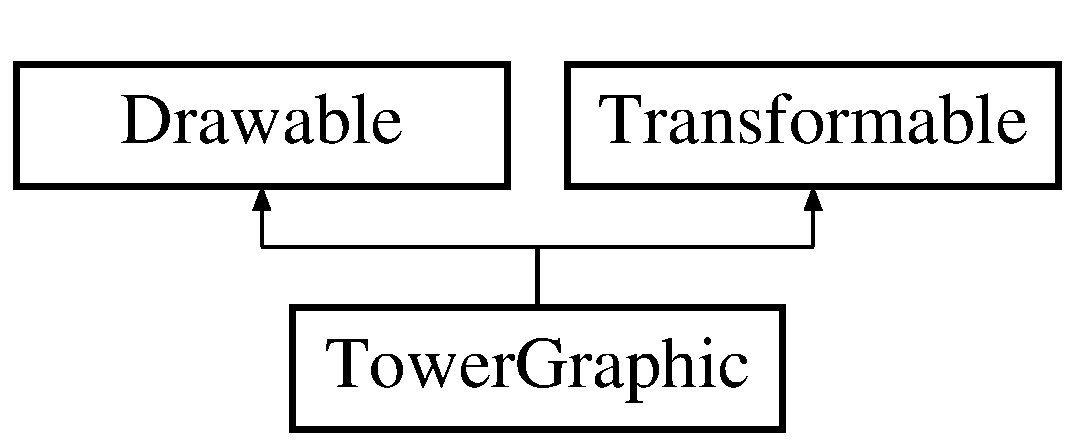
\includegraphics[height=2.000000cm]{class_tower_graphic}
\end{center}
\end{figure}
\subsection*{Public Member Functions}
\begin{DoxyCompactItemize}
\item 
\mbox{\Hypertarget{class_tower_graphic_a9fabddf8db14ad2aaf42d6e8f271ca70}\label{class_tower_graphic_a9fabddf8db14ad2aaf42d6e8f271ca70}} 
\mbox{\hyperlink{class_tower_graphic_a9fabddf8db14ad2aaf42d6e8f271ca70}{Tower\+Graphic}} ()
\begin{DoxyCompactList}\small\item\em Default constructor. \end{DoxyCompactList}\item 
void \mbox{\hyperlink{class_tower_graphic_a74c68c198252422789d39f7428130ae6}{load}} (const \mbox{\hyperlink{class_tower_manager}{Tower\+Manager}} \&tm)
\begin{DoxyCompactList}\small\item\em Prepares array of verticles according to data from tower manager. \end{DoxyCompactList}\item 
virtual void \mbox{\hyperlink{class_tower_graphic_acf08ab592132dc2992b5b4f02f26343b}{draw}} (sf\+::\+Render\+Target \&target, sf\+::\+Render\+States states) const
\begin{DoxyCompactList}\small\item\em Draws all towers to a target. \end{DoxyCompactList}\item 
\mbox{\Hypertarget{class_tower_graphic_a8f7c3e6d52c3b8a27137434c2b3ecb05}\label{class_tower_graphic_a8f7c3e6d52c3b8a27137434c2b3ecb05}} 
virtual \mbox{\hyperlink{class_tower_graphic_a8f7c3e6d52c3b8a27137434c2b3ecb05}{$\sim$\+Tower\+Graphic}} ()
\begin{DoxyCompactList}\small\item\em Destructor. \end{DoxyCompactList}\end{DoxyCompactItemize}


\subsection{Detailed Description}
Class managing drawing of towers. 

\subsection{Member Function Documentation}
\mbox{\Hypertarget{class_tower_graphic_acf08ab592132dc2992b5b4f02f26343b}\label{class_tower_graphic_acf08ab592132dc2992b5b4f02f26343b}} 
\index{Tower\+Graphic@{Tower\+Graphic}!draw@{draw}}
\index{draw@{draw}!Tower\+Graphic@{Tower\+Graphic}}
\subsubsection{\texorpdfstring{draw()}{draw()}}
{\footnotesize\ttfamily void Tower\+Graphic\+::draw (\begin{DoxyParamCaption}\item[{sf\+::\+Render\+Target \&}]{target,  }\item[{sf\+::\+Render\+States}]{states }\end{DoxyParamCaption}) const\hspace{0.3cm}{\ttfamily [virtual]}}



Draws all towers to a target. 

Inherited by sf\+:Dravable 
\begin{DoxyParams}{Parameters}
{\em target} & render target (typically window) \\
\hline
{\em states} & render states, such as transform, texture, etc. \\
\hline
\end{DoxyParams}
\mbox{\Hypertarget{class_tower_graphic_a74c68c198252422789d39f7428130ae6}\label{class_tower_graphic_a74c68c198252422789d39f7428130ae6}} 
\index{Tower\+Graphic@{Tower\+Graphic}!load@{load}}
\index{load@{load}!Tower\+Graphic@{Tower\+Graphic}}
\subsubsection{\texorpdfstring{load()}{load()}}
{\footnotesize\ttfamily void Tower\+Graphic\+::load (\begin{DoxyParamCaption}\item[{const \mbox{\hyperlink{class_tower_manager}{Tower\+Manager}} \&}]{tm }\end{DoxyParamCaption})}



Prepares array of verticles according to data from tower manager. 


\begin{DoxyParams}{Parameters}
{\em tm} & \mbox{\hyperlink{class_tower_manager}{Tower\+Manager}} object reference \\
\hline
\end{DoxyParams}


The documentation for this class was generated from the following files\+:\begin{DoxyCompactItemize}
\item 
Tower\+Defence/\+Graphics\+Handler/Tower\+Graphic.\+h\item 
Tower\+Defence/\+Graphics\+Handler/Tower\+Graphic.\+cpp\end{DoxyCompactItemize}

\hypertarget{class_tower_manager}{}\section{Tower\+Manager Class Reference}
\label{class_tower_manager}\index{Tower\+Manager@{Tower\+Manager}}


Class managing towers and theirs collection.  




{\ttfamily \#include $<$Tower\+Manager.\+h$>$}

\subsection*{Public Member Functions}
\begin{DoxyCompactItemize}
\item 
\mbox{\hyperlink{class_tower_manager_a709c5b86ae62f50820da54d535b83342}{Tower\+Manager}} (const \mbox{\hyperlink{class_map}{Map}} \&m)
\begin{DoxyCompactList}\small\item\em Constructor, creates manager object working at delivered map. \end{DoxyCompactList}\item 
\mbox{\Hypertarget{class_tower_manager_aa2c2765238a8747803334c164e767e41}\label{class_tower_manager_aa2c2765238a8747803334c164e767e41}} 
virtual \mbox{\hyperlink{class_tower_manager_aa2c2765238a8747803334c164e767e41}{$\sim$\+Tower\+Manager}} ()
\begin{DoxyCompactList}\small\item\em Destructor. \end{DoxyCompactList}\item 
bool \mbox{\hyperlink{class_tower_manager_a72ecf5954505cd071860b4468669c5bd}{buy}} (int x, int y)
\begin{DoxyCompactList}\small\item\em Buys tower in indicated coords. \end{DoxyCompactList}\item 
void \mbox{\hyperlink{class_tower_manager_ab1b232f3361916be0442ccdcaca30df6}{sell}} (const \mbox{\hyperlink{class_tower}{Tower}} \&t)
\begin{DoxyCompactList}\small\item\em Sells selected tower. \end{DoxyCompactList}\item 
void \mbox{\hyperlink{class_tower_manager_a3ccb8e040306022ef0ac2d54787a122d}{sell}} (int x, int y)
\begin{DoxyCompactList}\small\item\em Sells selected tower. \end{DoxyCompactList}\item 
bool \mbox{\hyperlink{class_tower_manager_aec10d63aa3de906706738c04fceb0ff7}{upgrade}} (const \mbox{\hyperlink{class_tower}{Tower}} \&t)
\begin{DoxyCompactList}\small\item\em Upgrades selected tower. \end{DoxyCompactList}\item 
bool \mbox{\hyperlink{class_tower_manager_a08071e4d7230bd316577086f787fffeb}{upgrade}} (int x, int y)
\begin{DoxyCompactList}\small\item\em Upgrades selected tower. \end{DoxyCompactList}\item 
\mbox{\hyperlink{class_tower}{Tower}} \& \mbox{\hyperlink{class_tower_manager_a05e8e2670b1b58f3d4f9851f431f08bc}{get}} (int x, int y)
\begin{DoxyCompactList}\small\item\em Gets tower from indicated location. \end{DoxyCompactList}\item 
\mbox{\hyperlink{class_tower}{Tower}} \& \mbox{\hyperlink{class_tower_manager_ad96e7abf6a9d512af64a86d7f44bf1a5}{operator\mbox{[}$\,$\mbox{]}}} (int i)
\begin{DoxyCompactList}\small\item\em Gets tower of indicated index. \end{DoxyCompactList}\item 
bool \mbox{\hyperlink{class_tower_manager_ab4943b63a4d5646ae6a951108732f4f6}{is\+Tower}} (int x, int y) const
\begin{DoxyCompactList}\small\item\em Checks if there is a tower in indicated coordinates. \end{DoxyCompactList}\item 
int \mbox{\hyperlink{class_tower_manager_a78683aa19991978f304fbea0b8e25890}{get\+Size}} () const
\begin{DoxyCompactList}\small\item\em Gets number of towers in collection. \end{DoxyCompactList}\item 
bool \mbox{\hyperlink{class_tower_manager_ad421cee3c30020aa02e770823dd1dab6}{update\+Graphic}} (\mbox{\hyperlink{class_tower_graphic}{Tower\+Graphic}} \&tg)
\begin{DoxyCompactList}\small\item\em Updates \mbox{\hyperlink{class_tower_graphic}{Tower\+Graphic}} object with new towers state. \end{DoxyCompactList}\item 
void \mbox{\hyperlink{class_tower_manager_a67c7741801ff0935ea2b0a6181768532}{Add\+Cash}} (uint v)
\begin{DoxyCompactList}\small\item\em Increases cash amount. \end{DoxyCompactList}\item 
std\+::string \mbox{\hyperlink{class_tower_manager_ae449833a3d381d3d616c35b1489ecd55}{Get\+Cash}} () const
\begin{DoxyCompactList}\small\item\em Gets cash amount. \end{DoxyCompactList}\item 
auto \mbox{\hyperlink{class_tower_manager_a90d1ce46145a7b52d50308ab29de5616}{begin}} () const
\begin{DoxyCompactList}\small\item\em Gets iterator set to begin of tower collection. \end{DoxyCompactList}\item 
auto \mbox{\hyperlink{class_tower_manager_a66cb83ad5d16ae63806b65d34768645e}{end}} () const
\begin{DoxyCompactList}\small\item\em Gets iterator set to end of tower collection. \end{DoxyCompactList}\end{DoxyCompactItemize}
\subsection*{Public Attributes}
\begin{DoxyCompactItemize}
\item 
\mbox{\Hypertarget{class_tower_manager_ac3b672da8534f42c9981df3fd55a9fbe}\label{class_tower_manager_ac3b672da8534f42c9981df3fd55a9fbe}} 
std\+::vector$<$ \mbox{\hyperlink{class_tower}{Tower}} $>$ \mbox{\hyperlink{class_tower_manager_ac3b672da8534f42c9981df3fd55a9fbe}{tab}}
\begin{DoxyCompactList}\small\item\em Collection of towers. \end{DoxyCompactList}\end{DoxyCompactItemize}


\subsection{Detailed Description}
Class managing towers and theirs collection. 

It provides methods to buying, upgrading and selling towers ~\newline
Also manages player cash 

\subsection{Constructor \& Destructor Documentation}
\mbox{\Hypertarget{class_tower_manager_a709c5b86ae62f50820da54d535b83342}\label{class_tower_manager_a709c5b86ae62f50820da54d535b83342}} 
\index{Tower\+Manager@{Tower\+Manager}!Tower\+Manager@{Tower\+Manager}}
\index{Tower\+Manager@{Tower\+Manager}!Tower\+Manager@{Tower\+Manager}}
\subsubsection{\texorpdfstring{Tower\+Manager()}{TowerManager()}}
{\footnotesize\ttfamily Tower\+Manager\+::\+Tower\+Manager (\begin{DoxyParamCaption}\item[{const \mbox{\hyperlink{class_map}{Map}} \&}]{m }\end{DoxyParamCaption})}



Constructor, creates manager object working at delivered map. 


\begin{DoxyParams}{Parameters}
{\em m} & logical map \\
\hline
\end{DoxyParams}


\subsection{Member Function Documentation}
\mbox{\Hypertarget{class_tower_manager_a67c7741801ff0935ea2b0a6181768532}\label{class_tower_manager_a67c7741801ff0935ea2b0a6181768532}} 
\index{Tower\+Manager@{Tower\+Manager}!Add\+Cash@{Add\+Cash}}
\index{Add\+Cash@{Add\+Cash}!Tower\+Manager@{Tower\+Manager}}
\subsubsection{\texorpdfstring{Add\+Cash()}{AddCash()}}
{\footnotesize\ttfamily void Tower\+Manager\+::\+Add\+Cash (\begin{DoxyParamCaption}\item[{uint}]{v }\end{DoxyParamCaption})}



Increases cash amount. 


\begin{DoxyParams}{Parameters}
{\em v} & income \\
\hline
\end{DoxyParams}
\mbox{\Hypertarget{class_tower_manager_a90d1ce46145a7b52d50308ab29de5616}\label{class_tower_manager_a90d1ce46145a7b52d50308ab29de5616}} 
\index{Tower\+Manager@{Tower\+Manager}!begin@{begin}}
\index{begin@{begin}!Tower\+Manager@{Tower\+Manager}}
\subsubsection{\texorpdfstring{begin()}{begin()}}
{\footnotesize\ttfamily auto Tower\+Manager\+::begin (\begin{DoxyParamCaption}{ }\end{DoxyParamCaption}) const\hspace{0.3cm}{\ttfamily [inline]}}



Gets iterator set to begin of tower collection. 

\begin{DoxyReturn}{Returns}
begin iterator 
\end{DoxyReturn}
\mbox{\Hypertarget{class_tower_manager_a72ecf5954505cd071860b4468669c5bd}\label{class_tower_manager_a72ecf5954505cd071860b4468669c5bd}} 
\index{Tower\+Manager@{Tower\+Manager}!buy@{buy}}
\index{buy@{buy}!Tower\+Manager@{Tower\+Manager}}
\subsubsection{\texorpdfstring{buy()}{buy()}}
{\footnotesize\ttfamily bool Tower\+Manager\+::buy (\begin{DoxyParamCaption}\item[{int}]{x,  }\item[{int}]{y }\end{DoxyParamCaption})}



Buys tower in indicated coords. 

\mbox{\hyperlink{class_tower}{Tower}} can be bougth only if choosen square is of empty terrain type and there are sufficient amount of cash 
\begin{DoxyParams}{Parameters}
{\em x} & x coordinate in squares \\
\hline
{\em y} & y coordinate in squares \\
\hline
\end{DoxyParams}
\begin{DoxyReturn}{Returns}
true if operation succeed, false otherwise 
\end{DoxyReturn}
\mbox{\Hypertarget{class_tower_manager_a66cb83ad5d16ae63806b65d34768645e}\label{class_tower_manager_a66cb83ad5d16ae63806b65d34768645e}} 
\index{Tower\+Manager@{Tower\+Manager}!end@{end}}
\index{end@{end}!Tower\+Manager@{Tower\+Manager}}
\subsubsection{\texorpdfstring{end()}{end()}}
{\footnotesize\ttfamily auto Tower\+Manager\+::end (\begin{DoxyParamCaption}{ }\end{DoxyParamCaption}) const\hspace{0.3cm}{\ttfamily [inline]}}



Gets iterator set to end of tower collection. 

\begin{DoxyReturn}{Returns}
end iterator 
\end{DoxyReturn}
\mbox{\Hypertarget{class_tower_manager_a05e8e2670b1b58f3d4f9851f431f08bc}\label{class_tower_manager_a05e8e2670b1b58f3d4f9851f431f08bc}} 
\index{Tower\+Manager@{Tower\+Manager}!get@{get}}
\index{get@{get}!Tower\+Manager@{Tower\+Manager}}
\subsubsection{\texorpdfstring{get()}{get()}}
{\footnotesize\ttfamily \mbox{\hyperlink{class_tower}{Tower}} \& Tower\+Manager\+::get (\begin{DoxyParamCaption}\item[{int}]{x,  }\item[{int}]{y }\end{DoxyParamCaption})}



Gets tower from indicated location. 


\begin{DoxyParams}{Parameters}
{\em x} & x coordinate in squares \\
\hline
{\em y} & y coordinate in squares \\
\hline
\end{DoxyParams}
\begin{DoxyReturn}{Returns}
tower reference 

tower of (-\/1,-\/1) coords if found none in indicated location 
\end{DoxyReturn}
\mbox{\Hypertarget{class_tower_manager_ae449833a3d381d3d616c35b1489ecd55}\label{class_tower_manager_ae449833a3d381d3d616c35b1489ecd55}} 
\index{Tower\+Manager@{Tower\+Manager}!Get\+Cash@{Get\+Cash}}
\index{Get\+Cash@{Get\+Cash}!Tower\+Manager@{Tower\+Manager}}
\subsubsection{\texorpdfstring{Get\+Cash()}{GetCash()}}
{\footnotesize\ttfamily std\+::string Tower\+Manager\+::\+Get\+Cash (\begin{DoxyParamCaption}{ }\end{DoxyParamCaption}) const}



Gets cash amount. 

\begin{DoxyReturn}{Returns}
cash amount 
\end{DoxyReturn}
\mbox{\Hypertarget{class_tower_manager_a78683aa19991978f304fbea0b8e25890}\label{class_tower_manager_a78683aa19991978f304fbea0b8e25890}} 
\index{Tower\+Manager@{Tower\+Manager}!get\+Size@{get\+Size}}
\index{get\+Size@{get\+Size}!Tower\+Manager@{Tower\+Manager}}
\subsubsection{\texorpdfstring{get\+Size()}{getSize()}}
{\footnotesize\ttfamily int Tower\+Manager\+::get\+Size (\begin{DoxyParamCaption}{ }\end{DoxyParamCaption}) const}



Gets number of towers in collection. 

\begin{DoxyReturn}{Returns}
size of tower collection 
\end{DoxyReturn}
\mbox{\Hypertarget{class_tower_manager_ab4943b63a4d5646ae6a951108732f4f6}\label{class_tower_manager_ab4943b63a4d5646ae6a951108732f4f6}} 
\index{Tower\+Manager@{Tower\+Manager}!is\+Tower@{is\+Tower}}
\index{is\+Tower@{is\+Tower}!Tower\+Manager@{Tower\+Manager}}
\subsubsection{\texorpdfstring{is\+Tower()}{isTower()}}
{\footnotesize\ttfamily bool Tower\+Manager\+::is\+Tower (\begin{DoxyParamCaption}\item[{int}]{x,  }\item[{int}]{y }\end{DoxyParamCaption}) const}



Checks if there is a tower in indicated coordinates. 


\begin{DoxyParams}{Parameters}
{\em x} & x coordinate in squares \\
\hline
{\em y} & y coordinate in squares \\
\hline
\end{DoxyParams}
\begin{DoxyReturn}{Returns}
true if there is a tower in indicated location, false otherwise 
\end{DoxyReturn}
\mbox{\Hypertarget{class_tower_manager_ad96e7abf6a9d512af64a86d7f44bf1a5}\label{class_tower_manager_ad96e7abf6a9d512af64a86d7f44bf1a5}} 
\index{Tower\+Manager@{Tower\+Manager}!operator\mbox{[}\mbox{]}@{operator[]}}
\index{operator\mbox{[}\mbox{]}@{operator[]}!Tower\+Manager@{Tower\+Manager}}
\subsubsection{\texorpdfstring{operator[]()}{operator[]()}}
{\footnotesize\ttfamily \mbox{\hyperlink{class_tower}{Tower}} \& Tower\+Manager\+::operator\mbox{[}$\,$\mbox{]} (\begin{DoxyParamCaption}\item[{int}]{i }\end{DoxyParamCaption})}



Gets tower of indicated index. 


\begin{DoxyParams}{Parameters}
{\em i} & tower index \\
\hline
\end{DoxyParams}
\begin{DoxyReturn}{Returns}
tower reference 
\end{DoxyReturn}
\mbox{\Hypertarget{class_tower_manager_ab1b232f3361916be0442ccdcaca30df6}\label{class_tower_manager_ab1b232f3361916be0442ccdcaca30df6}} 
\index{Tower\+Manager@{Tower\+Manager}!sell@{sell}}
\index{sell@{sell}!Tower\+Manager@{Tower\+Manager}}
\subsubsection{\texorpdfstring{sell()}{sell()}\hspace{0.1cm}{\footnotesize\ttfamily [1/2]}}
{\footnotesize\ttfamily void Tower\+Manager\+::sell (\begin{DoxyParamCaption}\item[{const \mbox{\hyperlink{class_tower}{Tower}} \&}]{t }\end{DoxyParamCaption})}



Sells selected tower. 


\begin{DoxyParams}{Parameters}
{\em t} & reference of selected tower \\
\hline
\end{DoxyParams}
\mbox{\Hypertarget{class_tower_manager_a3ccb8e040306022ef0ac2d54787a122d}\label{class_tower_manager_a3ccb8e040306022ef0ac2d54787a122d}} 
\index{Tower\+Manager@{Tower\+Manager}!sell@{sell}}
\index{sell@{sell}!Tower\+Manager@{Tower\+Manager}}
\subsubsection{\texorpdfstring{sell()}{sell()}\hspace{0.1cm}{\footnotesize\ttfamily [2/2]}}
{\footnotesize\ttfamily void Tower\+Manager\+::sell (\begin{DoxyParamCaption}\item[{int}]{x,  }\item[{int}]{y }\end{DoxyParamCaption})}



Sells selected tower. 


\begin{DoxyParams}{Parameters}
{\em x} & x coordinate in squares \\
\hline
{\em y} & y coordinate in squares \\
\hline
\end{DoxyParams}
\mbox{\Hypertarget{class_tower_manager_ad421cee3c30020aa02e770823dd1dab6}\label{class_tower_manager_ad421cee3c30020aa02e770823dd1dab6}} 
\index{Tower\+Manager@{Tower\+Manager}!update\+Graphic@{update\+Graphic}}
\index{update\+Graphic@{update\+Graphic}!Tower\+Manager@{Tower\+Manager}}
\subsubsection{\texorpdfstring{update\+Graphic()}{updateGraphic()}}
{\footnotesize\ttfamily bool Tower\+Manager\+::update\+Graphic (\begin{DoxyParamCaption}\item[{\mbox{\hyperlink{class_tower_graphic}{Tower\+Graphic}} \&}]{tg }\end{DoxyParamCaption})}



Updates \mbox{\hyperlink{class_tower_graphic}{Tower\+Graphic}} object with new towers state. 


\begin{DoxyParams}[1]{Parameters}
\mbox{\tt in,out}  & {\em tg} & reference to \mbox{\hyperlink{class_tower_graphic}{Tower\+Graphic}} object \\
\hline
\end{DoxyParams}
\begin{DoxyReturn}{Returns}
true if there were new data to update, false otherwise 
\end{DoxyReturn}
\mbox{\Hypertarget{class_tower_manager_aec10d63aa3de906706738c04fceb0ff7}\label{class_tower_manager_aec10d63aa3de906706738c04fceb0ff7}} 
\index{Tower\+Manager@{Tower\+Manager}!upgrade@{upgrade}}
\index{upgrade@{upgrade}!Tower\+Manager@{Tower\+Manager}}
\subsubsection{\texorpdfstring{upgrade()}{upgrade()}\hspace{0.1cm}{\footnotesize\ttfamily [1/2]}}
{\footnotesize\ttfamily bool Tower\+Manager\+::upgrade (\begin{DoxyParamCaption}\item[{const \mbox{\hyperlink{class_tower}{Tower}} \&}]{t }\end{DoxyParamCaption})}



Upgrades selected tower. 

\mbox{\hyperlink{class_tower}{Tower}} can be upgraded only if there are sufficient amount of cash 
\begin{DoxyParams}{Parameters}
{\em t} & reference of selected tower \\
\hline
\end{DoxyParams}
\begin{DoxyReturn}{Returns}
true if operation succeed, false otherwise 
\end{DoxyReturn}
\mbox{\Hypertarget{class_tower_manager_a08071e4d7230bd316577086f787fffeb}\label{class_tower_manager_a08071e4d7230bd316577086f787fffeb}} 
\index{Tower\+Manager@{Tower\+Manager}!upgrade@{upgrade}}
\index{upgrade@{upgrade}!Tower\+Manager@{Tower\+Manager}}
\subsubsection{\texorpdfstring{upgrade()}{upgrade()}\hspace{0.1cm}{\footnotesize\ttfamily [2/2]}}
{\footnotesize\ttfamily bool Tower\+Manager\+::upgrade (\begin{DoxyParamCaption}\item[{int}]{x,  }\item[{int}]{y }\end{DoxyParamCaption})}



Upgrades selected tower. 

\mbox{\hyperlink{class_tower}{Tower}} can be upgraded only if coordinates are proper and there are sufficient amount of cash 
\begin{DoxyParams}{Parameters}
{\em x} & x coordinate in squares \\
\hline
{\em y} & y coordinate in squares \\
\hline
\end{DoxyParams}
\begin{DoxyReturn}{Returns}
true if operation succeed, false otherwise 
\end{DoxyReturn}


The documentation for this class was generated from the following files\+:\begin{DoxyCompactItemize}
\item 
Tower\+Defence/\+Graphics\+Handler/Tower\+Manager.\+h\item 
Tower\+Defence/\+Graphics\+Handler/Tower\+Manager.\+cpp\end{DoxyCompactItemize}

\hypertarget{class_utils}{}\section{Utils Class Reference}
\label{class_utils}\index{Utils@{Utils}}


Class used for providing useful functionality.  




{\ttfamily \#include $<$Utils.\+hpp$>$}

\subsection*{Static Public Member Functions}
\begin{DoxyCompactItemize}
\item 
static std\+::vector$<$ std\+::string $>$ \mbox{\hyperlink{class_utils_a4b340ceb0cae184c4d42237716284b1b}{split}} (std\+::string to\+Split, std\+::string Separator=\char`\"{} \char`\"{})
\begin{DoxyCompactList}\small\item\em method used for splitting string \end{DoxyCompactList}\end{DoxyCompactItemize}


\subsection{Detailed Description}
Class used for providing useful functionality. 

\subsection{Member Function Documentation}
\mbox{\Hypertarget{class_utils_a4b340ceb0cae184c4d42237716284b1b}\label{class_utils_a4b340ceb0cae184c4d42237716284b1b}} 
\index{Utils@{Utils}!split@{split}}
\index{split@{split}!Utils@{Utils}}
\subsubsection{\texorpdfstring{split()}{split()}}
{\footnotesize\ttfamily std\+::vector$<$ std\+::string $>$ Utils\+::split (\begin{DoxyParamCaption}\item[{std\+::string}]{to\+Split,  }\item[{std\+::string}]{Separator = {\ttfamily \char`\"{}~\char`\"{}} }\end{DoxyParamCaption})\hspace{0.3cm}{\ttfamily [static]}}



method used for splitting string 


\begin{DoxyParams}{Parameters}
{\em string} & to split \\
\hline
{\em string} & separator \\
\hline
\end{DoxyParams}


The documentation for this class was generated from the following files\+:\begin{DoxyCompactItemize}
\item 
Tower\+Defence/\+Graphics\+Handler/Utils.\+hpp\item 
Tower\+Defence/\+Graphics\+Handler/Utils.\+cpp\end{DoxyCompactItemize}

\hypertarget{class_vampire}{}\section{Vampire Class Reference}
\label{class_vampire}\index{Vampire@{Vampire}}


Class representing vampire.  




{\ttfamily \#include $<$Enemy\+Designer.\+h$>$}

Inheritance diagram for Vampire\+:\begin{figure}[H]
\begin{center}
\leavevmode
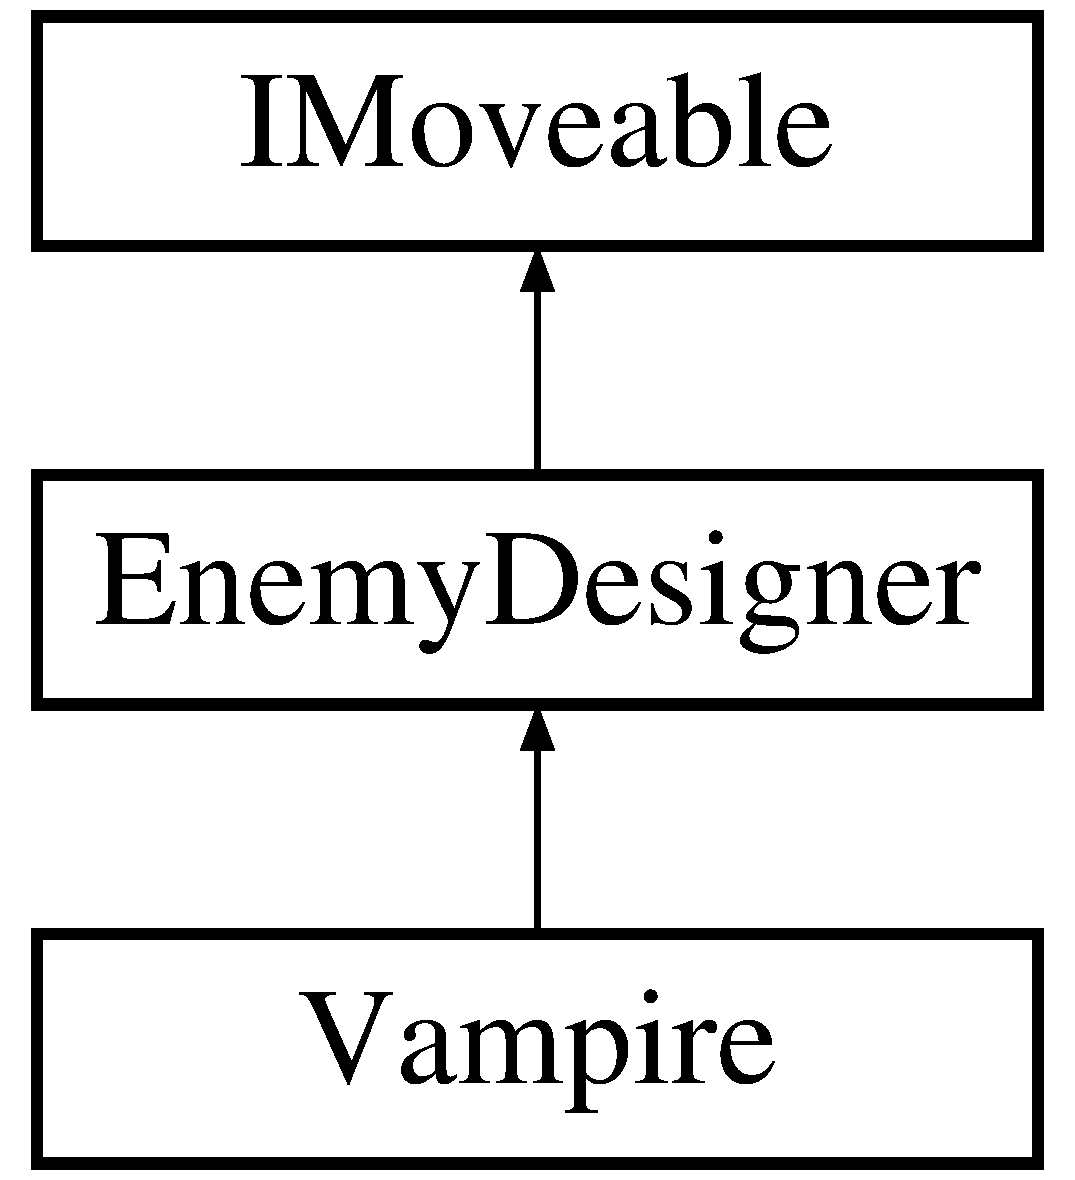
\includegraphics[height=3.000000cm]{class_vampire}
\end{center}
\end{figure}
\subsection*{Public Member Functions}
\begin{DoxyCompactItemize}
\item 
\mbox{\hyperlink{class_vampire_a5e4b1003b26311f3c248f87e6871ceb5}{Vampire}} (sf\+::\+Vector2f origin, sf\+::\+Vector2f dimensions, sf\+::\+Color color, sf\+::\+Vector2f texture\+Dimensions, std\+::string texture\+File=\char`\"{}vampire.\+png\char`\"{})
\begin{DoxyCompactList}\small\item\em constructor for vampire class \end{DoxyCompactList}\end{DoxyCompactItemize}
\subsection*{Additional Inherited Members}


\subsection{Detailed Description}
Class representing vampire. 

\subsection{Constructor \& Destructor Documentation}
\mbox{\Hypertarget{class_vampire_a5e4b1003b26311f3c248f87e6871ceb5}\label{class_vampire_a5e4b1003b26311f3c248f87e6871ceb5}} 
\index{Vampire@{Vampire}!Vampire@{Vampire}}
\index{Vampire@{Vampire}!Vampire@{Vampire}}
\subsubsection{\texorpdfstring{Vampire()}{Vampire()}}
{\footnotesize\ttfamily Vampire\+::\+Vampire (\begin{DoxyParamCaption}\item[{sf\+::\+Vector2f}]{origin,  }\item[{sf\+::\+Vector2f}]{dimensions,  }\item[{sf\+::\+Color}]{color,  }\item[{sf\+::\+Vector2f}]{texture\+Dimensions,  }\item[{std\+::string}]{texture\+File = {\ttfamily \char`\"{}vampire.png\char`\"{}} }\end{DoxyParamCaption})}



constructor for vampire class 


\begin{DoxyParams}{Parameters}
{\em origin} & point \\
\hline
{\em dimensions} & \\
\hline
{\em color} & \\
\hline
{\em texture} & dimensions \\
\hline
{\em file} & containing texture \\
\hline
\end{DoxyParams}


The documentation for this class was generated from the following files\+:\begin{DoxyCompactItemize}
\item 
Tower\+Defence/\+Graphics\+Handler/Enemy\+Designer.\+h\item 
Tower\+Defence/\+Graphics\+Handler/Enemy\+Designer.\+cpp\end{DoxyCompactItemize}

\hypertarget{class_wave}{}\section{Wave Class Reference}
\label{class_wave}\index{Wave@{Wave}}


Class representing waves of enemies in game.  




{\ttfamily \#include $<$Wave.\+h$>$}

\subsection*{Public Member Functions}
\begin{DoxyCompactItemize}
\item 
\mbox{\Hypertarget{class_wave_a6fb7dde8fde8d5b67d49f6cbefcecd6b}\label{class_wave_a6fb7dde8fde8d5b67d49f6cbefcecd6b}} 
int \mbox{\hyperlink{class_wave_a6fb7dde8fde8d5b67d49f6cbefcecd6b}{get\+Wave\+Id}} ()
\begin{DoxyCompactList}\small\item\em getter for wave id \end{DoxyCompactList}\item 
void \mbox{\hyperlink{class_wave_a27e3aec3e19fc4f4cbfdf3eb486062c0}{set\+Wave\+Id}} (int wave\+Id)
\begin{DoxyCompactList}\small\item\em setter for wave\textquotesingle{}s ID \end{DoxyCompactList}\item 
\mbox{\Hypertarget{class_wave_a3d8144ec0d6c0b0ede77ff59f54471aa}\label{class_wave_a3d8144ec0d6c0b0ede77ff59f54471aa}} 
\mbox{\hyperlink{class_wave_a3d8144ec0d6c0b0ede77ff59f54471aa}{Wave}} ()
\begin{DoxyCompactList}\small\item\em Constructor. \end{DoxyCompactList}\item 
\mbox{\hyperlink{class_wave_afbe28f8ee2238a9ead6aec5da1969618}{Wave}} (std\+::vector$<$ std\+::tuple$<$ int, \mbox{\hyperlink{class_enemy_designer}{Enemy\+Designer}} $\ast$, std\+::string $>$$>$ enemies\+Vector, int wave\+Id)
\begin{DoxyCompactList}\small\item\em Constructor with parameters. \end{DoxyCompactList}\item 
void \mbox{\hyperlink{class_wave_a78681a9dac7ede8d160be13c4027e9fd}{set\+Enemies}} (std\+::vector$<$ std\+::tuple$<$ int, \mbox{\hyperlink{class_enemy_designer}{Enemy\+Designer}} $\ast$, std\+::string $>$$>$ enemies\+Vector)
\begin{DoxyCompactList}\small\item\em method for setting enemy \end{DoxyCompactList}\item 
void \mbox{\hyperlink{class_wave_a751c1e868a8b9c3d3f41063cdd474eb4}{add\+Enemy}} (int number\+Of\+Enemies, \mbox{\hyperlink{class_enemy_designer}{Enemy\+Designer}} $\ast$enemy, std\+::string enemy\+Name)
\begin{DoxyCompactList}\small\item\em method adding enemies \end{DoxyCompactList}\item 
\mbox{\Hypertarget{class_wave_a6c8aea6a9da3db3b0546ff7316b9df6b}\label{class_wave_a6c8aea6a9da3db3b0546ff7316b9df6b}} 
void \mbox{\hyperlink{class_wave_a6c8aea6a9da3db3b0546ff7316b9df6b}{clear\+Enemies}} ()
\begin{DoxyCompactList}\small\item\em method for clearing vector of enemies \end{DoxyCompactList}\item 
\mbox{\Hypertarget{class_wave_a2d064fab7f420a917739346ffb8aa30d}\label{class_wave_a2d064fab7f420a917739346ffb8aa30d}} 
std\+::vector$<$ std\+::tuple$<$ int, \mbox{\hyperlink{class_enemy_designer}{Enemy\+Designer}} $\ast$, std\+::string $>$ $>$ \mbox{\hyperlink{class_wave_a2d064fab7f420a917739346ffb8aa30d}{get\+Enemies\+Vector}} ()
\begin{DoxyCompactList}\small\item\em getter for enemies vector \end{DoxyCompactList}\end{DoxyCompactItemize}
\subsection*{Protected Attributes}
\begin{DoxyCompactItemize}
\item 
\mbox{\Hypertarget{class_wave_aa18fc1c8a7981abb4e004825ece2bf84}\label{class_wave_aa18fc1c8a7981abb4e004825ece2bf84}} 
int {\bfseries wave\+Id}
\item 
\mbox{\Hypertarget{class_wave_a815713abfba3a012c83da2396826fff7}\label{class_wave_a815713abfba3a012c83da2396826fff7}} 
std\+::vector$<$ std\+::tuple$<$ int, \mbox{\hyperlink{class_enemy_designer}{Enemy\+Designer}} $\ast$, std\+::string $>$ $>$ {\bfseries enemies\+Vector}
\end{DoxyCompactItemize}


\subsection{Detailed Description}
Class representing waves of enemies in game. 

\subsection{Constructor \& Destructor Documentation}
\mbox{\Hypertarget{class_wave_afbe28f8ee2238a9ead6aec5da1969618}\label{class_wave_afbe28f8ee2238a9ead6aec5da1969618}} 
\index{Wave@{Wave}!Wave@{Wave}}
\index{Wave@{Wave}!Wave@{Wave}}
\subsubsection{\texorpdfstring{Wave()}{Wave()}}
{\footnotesize\ttfamily Wave\+::\+Wave (\begin{DoxyParamCaption}\item[{std\+::vector$<$ std\+::tuple$<$ int, \mbox{\hyperlink{class_enemy_designer}{Enemy\+Designer}} $\ast$, std\+::string $>$$>$}]{enemies\+Vector,  }\item[{int}]{wave\+Id }\end{DoxyParamCaption})}



Constructor with parameters. 


\begin{DoxyParams}{Parameters}
{\em vector} & of tuples representing enemies, their names and numbers \\
\hline
{\em wave\textquotesingle{}s} & id \\
\hline
\end{DoxyParams}


\subsection{Member Function Documentation}
\mbox{\Hypertarget{class_wave_a751c1e868a8b9c3d3f41063cdd474eb4}\label{class_wave_a751c1e868a8b9c3d3f41063cdd474eb4}} 
\index{Wave@{Wave}!add\+Enemy@{add\+Enemy}}
\index{add\+Enemy@{add\+Enemy}!Wave@{Wave}}
\subsubsection{\texorpdfstring{add\+Enemy()}{addEnemy()}}
{\footnotesize\ttfamily void Wave\+::add\+Enemy (\begin{DoxyParamCaption}\item[{int}]{number\+Of\+Enemy,  }\item[{\mbox{\hyperlink{class_enemy_designer}{Enemy\+Designer}} $\ast$}]{enemy,  }\item[{std\+::string}]{enemy\+Name }\end{DoxyParamCaption})}



method adding enemies 


\begin{DoxyParams}{Parameters}
{\em number} & of enemies \\
\hline
{\em pointer} & to enemy \\
\hline
{\em name} & of enemy \\
\hline
\end{DoxyParams}
\mbox{\Hypertarget{class_wave_a78681a9dac7ede8d160be13c4027e9fd}\label{class_wave_a78681a9dac7ede8d160be13c4027e9fd}} 
\index{Wave@{Wave}!set\+Enemies@{set\+Enemies}}
\index{set\+Enemies@{set\+Enemies}!Wave@{Wave}}
\subsubsection{\texorpdfstring{set\+Enemies()}{setEnemies()}}
{\footnotesize\ttfamily void Wave\+::set\+Enemies (\begin{DoxyParamCaption}\item[{std\+::vector$<$ std\+::tuple$<$ int, \mbox{\hyperlink{class_enemy_designer}{Enemy\+Designer}} $\ast$, std\+::string $>$$>$}]{enemies\+Vector }\end{DoxyParamCaption})}



method for setting enemy 


\begin{DoxyParams}{Parameters}
{\em vector} & of tuples (number of enemies, pointer to enemy, name of enemy \\
\hline
\end{DoxyParams}
\mbox{\Hypertarget{class_wave_a27e3aec3e19fc4f4cbfdf3eb486062c0}\label{class_wave_a27e3aec3e19fc4f4cbfdf3eb486062c0}} 
\index{Wave@{Wave}!set\+Wave\+Id@{set\+Wave\+Id}}
\index{set\+Wave\+Id@{set\+Wave\+Id}!Wave@{Wave}}
\subsubsection{\texorpdfstring{set\+Wave\+Id()}{setWaveId()}}
{\footnotesize\ttfamily void Wave\+::set\+Wave\+Id (\begin{DoxyParamCaption}\item[{int}]{wave\+Id }\end{DoxyParamCaption})}



setter for wave\textquotesingle{}s ID 


\begin{DoxyParams}{Parameters}
{\em wave\textquotesingle{}s} & id \\
\hline
\end{DoxyParams}


The documentation for this class was generated from the following files\+:\begin{DoxyCompactItemize}
\item 
Tower\+Defence/\+Graphics\+Handler/Wave.\+h\item 
Tower\+Defence/\+Graphics\+Handler/Wave.\+cpp\end{DoxyCompactItemize}

\hypertarget{classrapidxml_1_1xml__attribute}{}\section{rapidxml\+:\+:xml\+\_\+attribute$<$ Ch $>$ Class Template Reference}
\label{classrapidxml_1_1xml__attribute}\index{rapidxml\+::xml\+\_\+attribute$<$ Ch $>$@{rapidxml\+::xml\+\_\+attribute$<$ Ch $>$}}


{\ttfamily \#include $<$rapidxml.\+hpp$>$}

Inheritance diagram for rapidxml\+:\+:xml\+\_\+attribute$<$ Ch $>$\+:\begin{figure}[H]
\begin{center}
\leavevmode
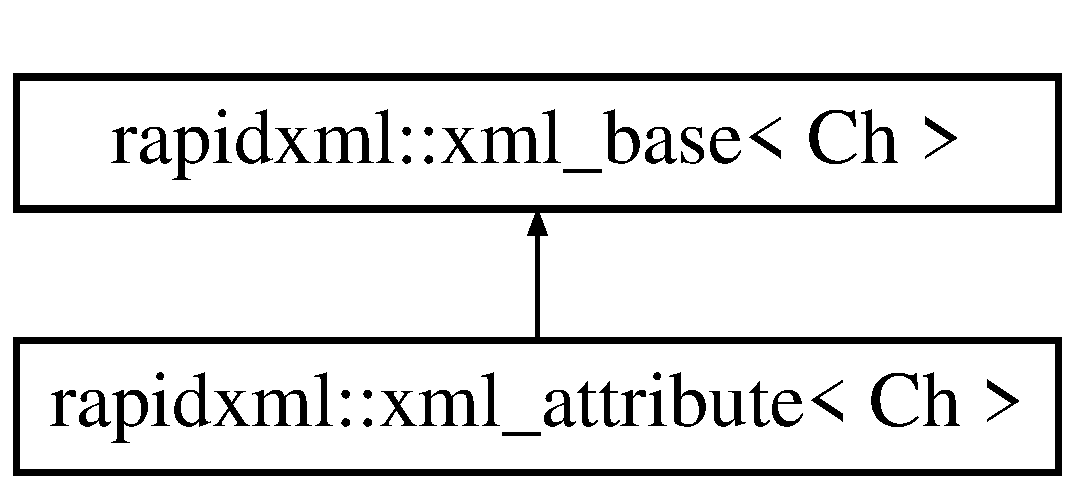
\includegraphics[height=2.000000cm]{classrapidxml_1_1xml__attribute}
\end{center}
\end{figure}
\subsection*{Public Member Functions}
\begin{DoxyCompactItemize}
\item 
\mbox{\hyperlink{classrapidxml_1_1xml__attribute_a26be291103917d3e8de110d46dd83816}{xml\+\_\+attribute}} ()
\item 
\mbox{\hyperlink{classrapidxml_1_1xml__document}{xml\+\_\+document}}$<$ Ch $>$ $\ast$ \mbox{\hyperlink{classrapidxml_1_1xml__attribute_ab0ff3bc7880a6969ddcf0bb1e0444077}{document}} () const
\item 
\mbox{\hyperlink{classrapidxml_1_1xml__attribute}{xml\+\_\+attribute}}$<$ Ch $>$ $\ast$ \mbox{\hyperlink{classrapidxml_1_1xml__attribute_abb0fb881f7247aefaec4b65b5eabc7ee}{previous\+\_\+attribute}} (const Ch $\ast$\mbox{\hyperlink{classrapidxml_1_1xml__base_aef8ae147fbee59209f714274afc80dc4}{name}}=0, std\+::size\+\_\+t \mbox{\hyperlink{classrapidxml_1_1xml__base_a20c8ffbe0c7a0b4231681ab8b99330a4}{name\+\_\+size}}=0, bool case\+\_\+sensitive=true) const
\item 
\mbox{\hyperlink{classrapidxml_1_1xml__attribute}{xml\+\_\+attribute}}$<$ Ch $>$ $\ast$ \mbox{\hyperlink{classrapidxml_1_1xml__attribute_affd0c8d0a9020df0998c507cae5474e5}{next\+\_\+attribute}} (const Ch $\ast$\mbox{\hyperlink{classrapidxml_1_1xml__base_aef8ae147fbee59209f714274afc80dc4}{name}}=0, std\+::size\+\_\+t \mbox{\hyperlink{classrapidxml_1_1xml__base_a20c8ffbe0c7a0b4231681ab8b99330a4}{name\+\_\+size}}=0, bool case\+\_\+sensitive=true) const
\end{DoxyCompactItemize}
\subsection*{Friends}
\begin{DoxyCompactItemize}
\item 
\mbox{\Hypertarget{classrapidxml_1_1xml__attribute_aa7e464ce3fe512598ff8dda47291941f}\label{classrapidxml_1_1xml__attribute_aa7e464ce3fe512598ff8dda47291941f}} 
class {\bfseries xml\+\_\+node$<$ Ch $>$}
\end{DoxyCompactItemize}
\subsection*{Additional Inherited Members}


\subsection{Detailed Description}
\subsubsection*{template$<$class Ch = char$>$\newline
class rapidxml\+::xml\+\_\+attribute$<$ Ch $>$}

Class representing attribute node of X\+ML document. Each attribute has name and value strings, which are available through \mbox{\hyperlink{classrapidxml_1_1xml__base_aef8ae147fbee59209f714274afc80dc4}{name()}} and \mbox{\hyperlink{classrapidxml_1_1xml__base_a6af65de5e59ac497cd69838f8a89d602}{value()}} functions (inherited from \mbox{\hyperlink{classrapidxml_1_1xml__base}{xml\+\_\+base}}). Note that after parse, both name and value of attribute will point to interior of source text used for parsing. Thus, this text must persist in memory for the lifetime of attribute. 
\begin{DoxyParams}{Parameters}
{\em Ch} & Character type to use. \\
\hline
\end{DoxyParams}


\subsection{Constructor \& Destructor Documentation}
\mbox{\Hypertarget{classrapidxml_1_1xml__attribute_a26be291103917d3e8de110d46dd83816}\label{classrapidxml_1_1xml__attribute_a26be291103917d3e8de110d46dd83816}} 
\index{rapidxml\+::xml\+\_\+attribute@{rapidxml\+::xml\+\_\+attribute}!xml\+\_\+attribute@{xml\+\_\+attribute}}
\index{xml\+\_\+attribute@{xml\+\_\+attribute}!rapidxml\+::xml\+\_\+attribute@{rapidxml\+::xml\+\_\+attribute}}
\subsubsection{\texorpdfstring{xml\+\_\+attribute()}{xml\_attribute()}}
{\footnotesize\ttfamily template$<$class Ch = char$>$ \\
\mbox{\hyperlink{classrapidxml_1_1xml__attribute}{rapidxml\+::xml\+\_\+attribute}}$<$ Ch $>$\+::\mbox{\hyperlink{classrapidxml_1_1xml__attribute}{xml\+\_\+attribute}} (\begin{DoxyParamCaption}{ }\end{DoxyParamCaption})\hspace{0.3cm}{\ttfamily [inline]}}

Constructs an empty attribute with the specified type. Consider using \mbox{\hyperlink{classrapidxml_1_1memory__pool}{memory\+\_\+pool}} of appropriate \mbox{\hyperlink{classrapidxml_1_1xml__document}{xml\+\_\+document}} if allocating attributes manually. 

\subsection{Member Function Documentation}
\mbox{\Hypertarget{classrapidxml_1_1xml__attribute_ab0ff3bc7880a6969ddcf0bb1e0444077}\label{classrapidxml_1_1xml__attribute_ab0ff3bc7880a6969ddcf0bb1e0444077}} 
\index{rapidxml\+::xml\+\_\+attribute@{rapidxml\+::xml\+\_\+attribute}!document@{document}}
\index{document@{document}!rapidxml\+::xml\+\_\+attribute@{rapidxml\+::xml\+\_\+attribute}}
\subsubsection{\texorpdfstring{document()}{document()}}
{\footnotesize\ttfamily template$<$class Ch = char$>$ \\
\mbox{\hyperlink{classrapidxml_1_1xml__document}{xml\+\_\+document}}$<$Ch$>$$\ast$ \mbox{\hyperlink{classrapidxml_1_1xml__attribute}{rapidxml\+::xml\+\_\+attribute}}$<$ Ch $>$\+::document (\begin{DoxyParamCaption}{ }\end{DoxyParamCaption}) const\hspace{0.3cm}{\ttfamily [inline]}}

Gets document of which attribute is a child. \begin{DoxyReturn}{Returns}
Pointer to document that contains this attribute, or 0 if there is no parent document. 
\end{DoxyReturn}
\mbox{\Hypertarget{classrapidxml_1_1xml__attribute_affd0c8d0a9020df0998c507cae5474e5}\label{classrapidxml_1_1xml__attribute_affd0c8d0a9020df0998c507cae5474e5}} 
\index{rapidxml\+::xml\+\_\+attribute@{rapidxml\+::xml\+\_\+attribute}!next\+\_\+attribute@{next\+\_\+attribute}}
\index{next\+\_\+attribute@{next\+\_\+attribute}!rapidxml\+::xml\+\_\+attribute@{rapidxml\+::xml\+\_\+attribute}}
\subsubsection{\texorpdfstring{next\+\_\+attribute()}{next\_attribute()}}
{\footnotesize\ttfamily template$<$class Ch = char$>$ \\
\mbox{\hyperlink{classrapidxml_1_1xml__attribute}{xml\+\_\+attribute}}$<$Ch$>$$\ast$ \mbox{\hyperlink{classrapidxml_1_1xml__attribute}{rapidxml\+::xml\+\_\+attribute}}$<$ Ch $>$\+::next\+\_\+attribute (\begin{DoxyParamCaption}\item[{const Ch $\ast$}]{name = {\ttfamily 0},  }\item[{std\+::size\+\_\+t}]{name\+\_\+size = {\ttfamily 0},  }\item[{bool}]{case\+\_\+sensitive = {\ttfamily true} }\end{DoxyParamCaption}) const\hspace{0.3cm}{\ttfamily [inline]}}

Gets next attribute, optionally matching attribute name. 
\begin{DoxyParams}{Parameters}
{\em name} & Name of attribute to find, or 0 to return next attribute regardless of its name; this string doesn\textquotesingle{}t have to be zero-\/terminated if name\+\_\+size is non-\/zero \\
\hline
{\em name\+\_\+size} & Size of name, in characters, or 0 to have size calculated automatically from string \\
\hline
{\em case\+\_\+sensitive} & Should name comparison be case-\/sensitive; non case-\/sensitive comparison works properly only for A\+S\+C\+II characters \\
\hline
\end{DoxyParams}
\begin{DoxyReturn}{Returns}
Pointer to found attribute, or 0 if not found. 
\end{DoxyReturn}
\mbox{\Hypertarget{classrapidxml_1_1xml__attribute_abb0fb881f7247aefaec4b65b5eabc7ee}\label{classrapidxml_1_1xml__attribute_abb0fb881f7247aefaec4b65b5eabc7ee}} 
\index{rapidxml\+::xml\+\_\+attribute@{rapidxml\+::xml\+\_\+attribute}!previous\+\_\+attribute@{previous\+\_\+attribute}}
\index{previous\+\_\+attribute@{previous\+\_\+attribute}!rapidxml\+::xml\+\_\+attribute@{rapidxml\+::xml\+\_\+attribute}}
\subsubsection{\texorpdfstring{previous\+\_\+attribute()}{previous\_attribute()}}
{\footnotesize\ttfamily template$<$class Ch = char$>$ \\
\mbox{\hyperlink{classrapidxml_1_1xml__attribute}{xml\+\_\+attribute}}$<$Ch$>$$\ast$ \mbox{\hyperlink{classrapidxml_1_1xml__attribute}{rapidxml\+::xml\+\_\+attribute}}$<$ Ch $>$\+::previous\+\_\+attribute (\begin{DoxyParamCaption}\item[{const Ch $\ast$}]{name = {\ttfamily 0},  }\item[{std\+::size\+\_\+t}]{name\+\_\+size = {\ttfamily 0},  }\item[{bool}]{case\+\_\+sensitive = {\ttfamily true} }\end{DoxyParamCaption}) const\hspace{0.3cm}{\ttfamily [inline]}}

Gets previous attribute, optionally matching attribute name. 
\begin{DoxyParams}{Parameters}
{\em name} & Name of attribute to find, or 0 to return previous attribute regardless of its name; this string doesn\textquotesingle{}t have to be zero-\/terminated if name\+\_\+size is non-\/zero \\
\hline
{\em name\+\_\+size} & Size of name, in characters, or 0 to have size calculated automatically from string \\
\hline
{\em case\+\_\+sensitive} & Should name comparison be case-\/sensitive; non case-\/sensitive comparison works properly only for A\+S\+C\+II characters \\
\hline
\end{DoxyParams}
\begin{DoxyReturn}{Returns}
Pointer to found attribute, or 0 if not found. 
\end{DoxyReturn}


The documentation for this class was generated from the following file\+:\begin{DoxyCompactItemize}
\item 
Tower\+Defence/\+Graphics\+Handler/\mbox{\hyperlink{rapidxml_8hpp}{rapidxml.\+hpp}}\end{DoxyCompactItemize}

\hypertarget{classrapidxml_1_1xml__base}{}\section{rapidxml\+:\+:xml\+\_\+base$<$ Ch $>$ Class Template Reference}
\label{classrapidxml_1_1xml__base}\index{rapidxml\+::xml\+\_\+base$<$ Ch $>$@{rapidxml\+::xml\+\_\+base$<$ Ch $>$}}


{\ttfamily \#include $<$rapidxml.\+hpp$>$}

Inheritance diagram for rapidxml\+:\+:xml\+\_\+base$<$ Ch $>$\+:\begin{figure}[H]
\begin{center}
\leavevmode
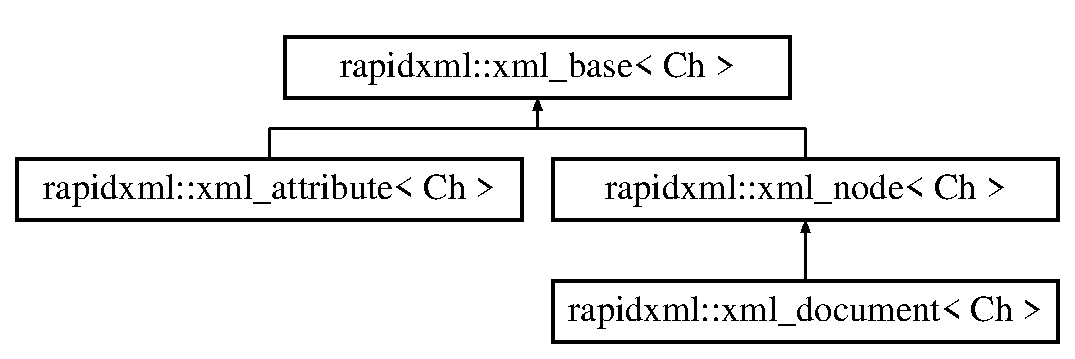
\includegraphics[height=3.000000cm]{classrapidxml_1_1xml__base}
\end{center}
\end{figure}
\subsection*{Public Member Functions}
\begin{DoxyCompactItemize}
\item 
Ch $\ast$ \mbox{\hyperlink{classrapidxml_1_1xml__base_aef8ae147fbee59209f714274afc80dc4}{name}} () const
\item 
std\+::size\+\_\+t \mbox{\hyperlink{classrapidxml_1_1xml__base_a20c8ffbe0c7a0b4231681ab8b99330a4}{name\+\_\+size}} () const
\item 
Ch $\ast$ \mbox{\hyperlink{classrapidxml_1_1xml__base_a6af65de5e59ac497cd69838f8a89d602}{value}} () const
\item 
std\+::size\+\_\+t \mbox{\hyperlink{classrapidxml_1_1xml__base_a2eb123d471b1567fa4832b6ee2b75493}{value\+\_\+size}} () const
\item 
void \mbox{\hyperlink{classrapidxml_1_1xml__base_ae55060ae958c6e6465d6c8db852ec6ce}{name}} (const Ch $\ast$name, std\+::size\+\_\+t size)
\item 
void \mbox{\hyperlink{classrapidxml_1_1xml__base_a4611ddc82ac83a527c65606600eb2a0d}{name}} (const Ch $\ast$name)
\item 
void \mbox{\hyperlink{classrapidxml_1_1xml__base_a3b183c2db7022a6d30494dd2f0ac11e9}{value}} (const Ch $\ast$value, std\+::size\+\_\+t size)
\item 
void \mbox{\hyperlink{classrapidxml_1_1xml__base_a81e63ec4bfd2d7ef0a6c2ed49be6e623}{value}} (const Ch $\ast$value)
\item 
\mbox{\hyperlink{classrapidxml_1_1xml__node}{xml\+\_\+node}}$<$ Ch $>$ $\ast$ \mbox{\hyperlink{classrapidxml_1_1xml__base_aa807062868d671a8c798d9d1bf016988}{parent}} () const
\end{DoxyCompactItemize}
\subsection*{Static Protected Member Functions}
\begin{DoxyCompactItemize}
\item 
\mbox{\Hypertarget{classrapidxml_1_1xml__base_ad96ff6b1e41dab3ff60b9bc4df769a75}\label{classrapidxml_1_1xml__base_ad96ff6b1e41dab3ff60b9bc4df769a75}} 
static Ch $\ast$ {\bfseries nullstr} ()
\end{DoxyCompactItemize}
\subsection*{Protected Attributes}
\begin{DoxyCompactItemize}
\item 
\mbox{\Hypertarget{classrapidxml_1_1xml__base_afd9851ed43e14619db0d7075ef8e9e8a}\label{classrapidxml_1_1xml__base_afd9851ed43e14619db0d7075ef8e9e8a}} 
Ch $\ast$ {\bfseries m\+\_\+name}
\item 
\mbox{\Hypertarget{classrapidxml_1_1xml__base_a278a1ea63b0b70219b946cec47fa00ea}\label{classrapidxml_1_1xml__base_a278a1ea63b0b70219b946cec47fa00ea}} 
Ch $\ast$ {\bfseries m\+\_\+value}
\item 
\mbox{\Hypertarget{classrapidxml_1_1xml__base_a5a8c76a7274b4180213796422c4df76f}\label{classrapidxml_1_1xml__base_a5a8c76a7274b4180213796422c4df76f}} 
std\+::size\+\_\+t {\bfseries m\+\_\+name\+\_\+size}
\item 
\mbox{\Hypertarget{classrapidxml_1_1xml__base_aa3a49d8ceddb8a8d7edb773a2226b89c}\label{classrapidxml_1_1xml__base_aa3a49d8ceddb8a8d7edb773a2226b89c}} 
std\+::size\+\_\+t {\bfseries m\+\_\+value\+\_\+size}
\item 
\mbox{\Hypertarget{classrapidxml_1_1xml__base_a90d5f660f078f66563fd7b2d8387ccb0}\label{classrapidxml_1_1xml__base_a90d5f660f078f66563fd7b2d8387ccb0}} 
\mbox{\hyperlink{classrapidxml_1_1xml__node}{xml\+\_\+node}}$<$ Ch $>$ $\ast$ {\bfseries m\+\_\+parent}
\end{DoxyCompactItemize}


\subsection{Detailed Description}
\subsubsection*{template$<$class Ch = char$>$\newline
class rapidxml\+::xml\+\_\+base$<$ Ch $>$}

Base class for \mbox{\hyperlink{classrapidxml_1_1xml__node}{xml\+\_\+node}} and \mbox{\hyperlink{classrapidxml_1_1xml__attribute}{xml\+\_\+attribute}} implementing common functions\+: \mbox{\hyperlink{classrapidxml_1_1xml__base_aef8ae147fbee59209f714274afc80dc4}{name()}}, \mbox{\hyperlink{classrapidxml_1_1xml__base_a20c8ffbe0c7a0b4231681ab8b99330a4}{name\+\_\+size()}}, \mbox{\hyperlink{classrapidxml_1_1xml__base_a6af65de5e59ac497cd69838f8a89d602}{value()}}, \mbox{\hyperlink{classrapidxml_1_1xml__base_a2eb123d471b1567fa4832b6ee2b75493}{value\+\_\+size()}} and \mbox{\hyperlink{classrapidxml_1_1xml__base_aa807062868d671a8c798d9d1bf016988}{parent()}}. 
\begin{DoxyParams}{Parameters}
{\em Ch} & Character type to use \\
\hline
\end{DoxyParams}


\subsection{Member Function Documentation}
\mbox{\Hypertarget{classrapidxml_1_1xml__base_aef8ae147fbee59209f714274afc80dc4}\label{classrapidxml_1_1xml__base_aef8ae147fbee59209f714274afc80dc4}} 
\index{rapidxml\+::xml\+\_\+base@{rapidxml\+::xml\+\_\+base}!name@{name}}
\index{name@{name}!rapidxml\+::xml\+\_\+base@{rapidxml\+::xml\+\_\+base}}
\subsubsection{\texorpdfstring{name()}{name()}\hspace{0.1cm}{\footnotesize\ttfamily [1/3]}}
{\footnotesize\ttfamily template$<$class Ch  = char$>$ \\
Ch$\ast$ \mbox{\hyperlink{classrapidxml_1_1xml__base}{rapidxml\+::xml\+\_\+base}}$<$ Ch $>$\+::name (\begin{DoxyParamCaption}{ }\end{DoxyParamCaption}) const\hspace{0.3cm}{\ttfamily [inline]}}

Gets name of the node. Interpretation of name depends on type of node. Note that name will not be zero-\/terminated if rapidxml\+::parse\+\_\+no\+\_\+string\+\_\+terminators option was selected during parse. ~\newline
~\newline
 Use \mbox{\hyperlink{classrapidxml_1_1xml__base_a20c8ffbe0c7a0b4231681ab8b99330a4}{name\+\_\+size()}} function to determine length of the name. \begin{DoxyReturn}{Returns}
Name of node, or empty string if node has no name. 
\end{DoxyReturn}
\mbox{\Hypertarget{classrapidxml_1_1xml__base_ae55060ae958c6e6465d6c8db852ec6ce}\label{classrapidxml_1_1xml__base_ae55060ae958c6e6465d6c8db852ec6ce}} 
\index{rapidxml\+::xml\+\_\+base@{rapidxml\+::xml\+\_\+base}!name@{name}}
\index{name@{name}!rapidxml\+::xml\+\_\+base@{rapidxml\+::xml\+\_\+base}}
\subsubsection{\texorpdfstring{name()}{name()}\hspace{0.1cm}{\footnotesize\ttfamily [2/3]}}
{\footnotesize\ttfamily template$<$class Ch  = char$>$ \\
void \mbox{\hyperlink{classrapidxml_1_1xml__base}{rapidxml\+::xml\+\_\+base}}$<$ Ch $>$\+::name (\begin{DoxyParamCaption}\item[{const Ch $\ast$}]{name,  }\item[{std\+::size\+\_\+t}]{size }\end{DoxyParamCaption})\hspace{0.3cm}{\ttfamily [inline]}}

Sets name of node to a non zero-\/terminated string. See ownership\+\_\+of\+\_\+strings. ~\newline
~\newline
 Note that node does not own its name or value, it only stores a pointer to it. It will not delete or otherwise free the pointer on destruction. It is reponsibility of the user to properly manage lifetime of the string. The easiest way to achieve it is to use \mbox{\hyperlink{classrapidxml_1_1memory__pool}{memory\+\_\+pool}} of the document to allocate the string -\/ on destruction of the document the string will be automatically freed. ~\newline
~\newline
 Size of name must be specified separately, because name does not have to be zero terminated. Use \mbox{\hyperlink{classrapidxml_1_1xml__base_a4611ddc82ac83a527c65606600eb2a0d}{name(const Ch $\ast$)}} function to have the length automatically calculated (string must be zero terminated). 
\begin{DoxyParams}{Parameters}
{\em name} & Name of node to set. Does not have to be zero terminated. \\
\hline
{\em size} & Size of name, in characters. This does not include zero terminator, if one is present. \\
\hline
\end{DoxyParams}
\mbox{\Hypertarget{classrapidxml_1_1xml__base_a4611ddc82ac83a527c65606600eb2a0d}\label{classrapidxml_1_1xml__base_a4611ddc82ac83a527c65606600eb2a0d}} 
\index{rapidxml\+::xml\+\_\+base@{rapidxml\+::xml\+\_\+base}!name@{name}}
\index{name@{name}!rapidxml\+::xml\+\_\+base@{rapidxml\+::xml\+\_\+base}}
\subsubsection{\texorpdfstring{name()}{name()}\hspace{0.1cm}{\footnotesize\ttfamily [3/3]}}
{\footnotesize\ttfamily template$<$class Ch  = char$>$ \\
void \mbox{\hyperlink{classrapidxml_1_1xml__base}{rapidxml\+::xml\+\_\+base}}$<$ Ch $>$\+::name (\begin{DoxyParamCaption}\item[{const Ch $\ast$}]{name }\end{DoxyParamCaption})\hspace{0.3cm}{\ttfamily [inline]}}

Sets name of node to a zero-\/terminated string. See also ownership\+\_\+of\+\_\+strings and \mbox{\hyperlink{classrapidxml_1_1xml__base_ae55060ae958c6e6465d6c8db852ec6ce}{xml\+\_\+node\+::name(const Ch $\ast$, std\+::size\+\_\+t)}}. 
\begin{DoxyParams}{Parameters}
{\em name} & Name of node to set. Must be zero terminated. \\
\hline
\end{DoxyParams}
\mbox{\Hypertarget{classrapidxml_1_1xml__base_a20c8ffbe0c7a0b4231681ab8b99330a4}\label{classrapidxml_1_1xml__base_a20c8ffbe0c7a0b4231681ab8b99330a4}} 
\index{rapidxml\+::xml\+\_\+base@{rapidxml\+::xml\+\_\+base}!name\+\_\+size@{name\+\_\+size}}
\index{name\+\_\+size@{name\+\_\+size}!rapidxml\+::xml\+\_\+base@{rapidxml\+::xml\+\_\+base}}
\subsubsection{\texorpdfstring{name\+\_\+size()}{name\_size()}}
{\footnotesize\ttfamily template$<$class Ch  = char$>$ \\
std\+::size\+\_\+t \mbox{\hyperlink{classrapidxml_1_1xml__base}{rapidxml\+::xml\+\_\+base}}$<$ Ch $>$\+::name\+\_\+size (\begin{DoxyParamCaption}{ }\end{DoxyParamCaption}) const\hspace{0.3cm}{\ttfamily [inline]}}

Gets size of node name, not including terminator character. This function works correctly irrespective of whether name is or is not zero terminated. \begin{DoxyReturn}{Returns}
Size of node name, in characters. 
\end{DoxyReturn}
\mbox{\Hypertarget{classrapidxml_1_1xml__base_aa807062868d671a8c798d9d1bf016988}\label{classrapidxml_1_1xml__base_aa807062868d671a8c798d9d1bf016988}} 
\index{rapidxml\+::xml\+\_\+base@{rapidxml\+::xml\+\_\+base}!parent@{parent}}
\index{parent@{parent}!rapidxml\+::xml\+\_\+base@{rapidxml\+::xml\+\_\+base}}
\subsubsection{\texorpdfstring{parent()}{parent()}}
{\footnotesize\ttfamily template$<$class Ch  = char$>$ \\
\mbox{\hyperlink{classrapidxml_1_1xml__node}{xml\+\_\+node}}$<$Ch$>$$\ast$ \mbox{\hyperlink{classrapidxml_1_1xml__base}{rapidxml\+::xml\+\_\+base}}$<$ Ch $>$\+::parent (\begin{DoxyParamCaption}{ }\end{DoxyParamCaption}) const\hspace{0.3cm}{\ttfamily [inline]}}

Gets node parent. \begin{DoxyReturn}{Returns}
Pointer to parent node, or 0 if there is no parent. 
\end{DoxyReturn}
\mbox{\Hypertarget{classrapidxml_1_1xml__base_a6af65de5e59ac497cd69838f8a89d602}\label{classrapidxml_1_1xml__base_a6af65de5e59ac497cd69838f8a89d602}} 
\index{rapidxml\+::xml\+\_\+base@{rapidxml\+::xml\+\_\+base}!value@{value}}
\index{value@{value}!rapidxml\+::xml\+\_\+base@{rapidxml\+::xml\+\_\+base}}
\subsubsection{\texorpdfstring{value()}{value()}\hspace{0.1cm}{\footnotesize\ttfamily [1/3]}}
{\footnotesize\ttfamily template$<$class Ch  = char$>$ \\
Ch$\ast$ \mbox{\hyperlink{classrapidxml_1_1xml__base}{rapidxml\+::xml\+\_\+base}}$<$ Ch $>$\+::value (\begin{DoxyParamCaption}{ }\end{DoxyParamCaption}) const\hspace{0.3cm}{\ttfamily [inline]}}

Gets value of node. Interpretation of value depends on type of node. Note that value will not be zero-\/terminated if rapidxml\+::parse\+\_\+no\+\_\+string\+\_\+terminators option was selected during parse. ~\newline
~\newline
 Use \mbox{\hyperlink{classrapidxml_1_1xml__base_a2eb123d471b1567fa4832b6ee2b75493}{value\+\_\+size()}} function to determine length of the value. \begin{DoxyReturn}{Returns}
Value of node, or empty string if node has no value. 
\end{DoxyReturn}
\mbox{\Hypertarget{classrapidxml_1_1xml__base_a3b183c2db7022a6d30494dd2f0ac11e9}\label{classrapidxml_1_1xml__base_a3b183c2db7022a6d30494dd2f0ac11e9}} 
\index{rapidxml\+::xml\+\_\+base@{rapidxml\+::xml\+\_\+base}!value@{value}}
\index{value@{value}!rapidxml\+::xml\+\_\+base@{rapidxml\+::xml\+\_\+base}}
\subsubsection{\texorpdfstring{value()}{value()}\hspace{0.1cm}{\footnotesize\ttfamily [2/3]}}
{\footnotesize\ttfamily template$<$class Ch  = char$>$ \\
void \mbox{\hyperlink{classrapidxml_1_1xml__base}{rapidxml\+::xml\+\_\+base}}$<$ Ch $>$\+::value (\begin{DoxyParamCaption}\item[{const Ch $\ast$}]{value,  }\item[{std\+::size\+\_\+t}]{size }\end{DoxyParamCaption})\hspace{0.3cm}{\ttfamily [inline]}}

Sets value of node to a non zero-\/terminated string. See ownership\+\_\+of\+\_\+strings. ~\newline
~\newline
 Note that node does not own its name or value, it only stores a pointer to it. It will not delete or otherwise free the pointer on destruction. It is reponsibility of the user to properly manage lifetime of the string. The easiest way to achieve it is to use \mbox{\hyperlink{classrapidxml_1_1memory__pool}{memory\+\_\+pool}} of the document to allocate the string -\/ on destruction of the document the string will be automatically freed. ~\newline
~\newline
 Size of value must be specified separately, because it does not have to be zero terminated. Use \mbox{\hyperlink{classrapidxml_1_1xml__base_a81e63ec4bfd2d7ef0a6c2ed49be6e623}{value(const Ch $\ast$)}} function to have the length automatically calculated (string must be zero terminated). ~\newline
~\newline
 If an element has a child node of type node\+\_\+data, it will take precedence over element value when printing. If you want to manipulate data of elements using values, use parser flag rapidxml\+::parse\+\_\+no\+\_\+data\+\_\+nodes to prevent creation of data nodes by the parser. 
\begin{DoxyParams}{Parameters}
{\em value} & value of node to set. Does not have to be zero terminated. \\
\hline
{\em size} & Size of value, in characters. This does not include zero terminator, if one is present. \\
\hline
\end{DoxyParams}
\mbox{\Hypertarget{classrapidxml_1_1xml__base_a81e63ec4bfd2d7ef0a6c2ed49be6e623}\label{classrapidxml_1_1xml__base_a81e63ec4bfd2d7ef0a6c2ed49be6e623}} 
\index{rapidxml\+::xml\+\_\+base@{rapidxml\+::xml\+\_\+base}!value@{value}}
\index{value@{value}!rapidxml\+::xml\+\_\+base@{rapidxml\+::xml\+\_\+base}}
\subsubsection{\texorpdfstring{value()}{value()}\hspace{0.1cm}{\footnotesize\ttfamily [3/3]}}
{\footnotesize\ttfamily template$<$class Ch  = char$>$ \\
void \mbox{\hyperlink{classrapidxml_1_1xml__base}{rapidxml\+::xml\+\_\+base}}$<$ Ch $>$\+::value (\begin{DoxyParamCaption}\item[{const Ch $\ast$}]{value }\end{DoxyParamCaption})\hspace{0.3cm}{\ttfamily [inline]}}

Sets value of node to a zero-\/terminated string. See also ownership\+\_\+of\+\_\+strings and \mbox{\hyperlink{classrapidxml_1_1xml__base_a3b183c2db7022a6d30494dd2f0ac11e9}{xml\+\_\+node\+::value(const Ch $\ast$, std\+::size\+\_\+t)}}. 
\begin{DoxyParams}{Parameters}
{\em value} & Vame of node to set. Must be zero terminated. \\
\hline
\end{DoxyParams}
\mbox{\Hypertarget{classrapidxml_1_1xml__base_a2eb123d471b1567fa4832b6ee2b75493}\label{classrapidxml_1_1xml__base_a2eb123d471b1567fa4832b6ee2b75493}} 
\index{rapidxml\+::xml\+\_\+base@{rapidxml\+::xml\+\_\+base}!value\+\_\+size@{value\+\_\+size}}
\index{value\+\_\+size@{value\+\_\+size}!rapidxml\+::xml\+\_\+base@{rapidxml\+::xml\+\_\+base}}
\subsubsection{\texorpdfstring{value\+\_\+size()}{value\_size()}}
{\footnotesize\ttfamily template$<$class Ch  = char$>$ \\
std\+::size\+\_\+t \mbox{\hyperlink{classrapidxml_1_1xml__base}{rapidxml\+::xml\+\_\+base}}$<$ Ch $>$\+::value\+\_\+size (\begin{DoxyParamCaption}{ }\end{DoxyParamCaption}) const\hspace{0.3cm}{\ttfamily [inline]}}

Gets size of node value, not including terminator character. This function works correctly irrespective of whether value is or is not zero terminated. \begin{DoxyReturn}{Returns}
Size of node value, in characters. 
\end{DoxyReturn}


The documentation for this class was generated from the following file\+:\begin{DoxyCompactItemize}
\item 
Tower\+Defence/\+Graphics\+Handler/\mbox{\hyperlink{rapidxml_8hpp}{rapidxml.\+hpp}}\end{DoxyCompactItemize}

\hypertarget{classrapidxml_1_1xml__document}{}\section{rapidxml\+:\+:xml\+\_\+document$<$ Ch $>$ Class Template Reference}
\label{classrapidxml_1_1xml__document}\index{rapidxml\+::xml\+\_\+document$<$ Ch $>$@{rapidxml\+::xml\+\_\+document$<$ Ch $>$}}


{\ttfamily \#include $<$rapidxml.\+hpp$>$}

Inheritance diagram for rapidxml\+:\+:xml\+\_\+document$<$ Ch $>$\+:\begin{figure}[H]
\begin{center}
\leavevmode
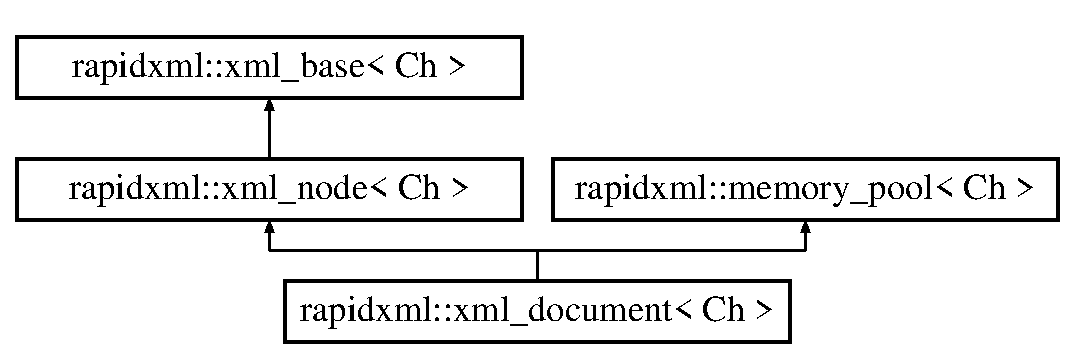
\includegraphics[height=3.000000cm]{classrapidxml_1_1xml__document}
\end{center}
\end{figure}
\subsection*{Public Member Functions}
\begin{DoxyCompactItemize}
\item 
\mbox{\Hypertarget{classrapidxml_1_1xml__document_aae8841b15085ba8f32ff46587ace28f5}\label{classrapidxml_1_1xml__document_aae8841b15085ba8f32ff46587ace28f5}} 
\mbox{\hyperlink{classrapidxml_1_1xml__document_aae8841b15085ba8f32ff46587ace28f5}{xml\+\_\+document}} ()
\begin{DoxyCompactList}\small\item\em Constructs empty X\+ML document. \end{DoxyCompactList}\item 
{\footnotesize template$<$int Flags$>$ }\\void \mbox{\hyperlink{classrapidxml_1_1xml__document_ac6e73ff9ac323bf5a370c38feb03a6b1}{parse}} (Ch $\ast$text)
\item 
void \mbox{\hyperlink{classrapidxml_1_1xml__document_a826929ff54242532198701f19ff5f83f}{clear}} ()
\end{DoxyCompactItemize}
\subsection*{Additional Inherited Members}


\subsection{Detailed Description}
\subsubsection*{template$<$class Ch = char$>$\newline
class rapidxml\+::xml\+\_\+document$<$ Ch $>$}

This class represents root of the D\+OM hierarchy. It is also an \mbox{\hyperlink{classrapidxml_1_1xml__node}{xml\+\_\+node}} and a \mbox{\hyperlink{classrapidxml_1_1memory__pool}{memory\+\_\+pool}} through public inheritance. Use \mbox{\hyperlink{classrapidxml_1_1xml__document_ac6e73ff9ac323bf5a370c38feb03a6b1}{parse()}} function to build a D\+OM tree from a zero-\/terminated X\+ML text string. \mbox{\hyperlink{classrapidxml_1_1xml__document_ac6e73ff9ac323bf5a370c38feb03a6b1}{parse()}} function allocates memory for nodes and attributes by using functions of \mbox{\hyperlink{classrapidxml_1_1xml__document}{xml\+\_\+document}}, which are inherited from \mbox{\hyperlink{classrapidxml_1_1memory__pool}{memory\+\_\+pool}}. To access root node of the document, use the document itself, as if it was an \mbox{\hyperlink{classrapidxml_1_1xml__node}{xml\+\_\+node}}. 
\begin{DoxyParams}{Parameters}
{\em Ch} & Character type to use. \\
\hline
\end{DoxyParams}


\subsection{Member Function Documentation}
\mbox{\Hypertarget{classrapidxml_1_1xml__document_a826929ff54242532198701f19ff5f83f}\label{classrapidxml_1_1xml__document_a826929ff54242532198701f19ff5f83f}} 
\index{rapidxml\+::xml\+\_\+document@{rapidxml\+::xml\+\_\+document}!clear@{clear}}
\index{clear@{clear}!rapidxml\+::xml\+\_\+document@{rapidxml\+::xml\+\_\+document}}
\subsubsection{\texorpdfstring{clear()}{clear()}}
{\footnotesize\ttfamily template$<$class Ch  = char$>$ \\
void \mbox{\hyperlink{classrapidxml_1_1xml__document}{rapidxml\+::xml\+\_\+document}}$<$ Ch $>$\+::clear (\begin{DoxyParamCaption}{ }\end{DoxyParamCaption})\hspace{0.3cm}{\ttfamily [inline]}}

Clears the document by deleting all nodes and clearing the memory pool. All nodes owned by document pool are destroyed. \mbox{\Hypertarget{classrapidxml_1_1xml__document_ac6e73ff9ac323bf5a370c38feb03a6b1}\label{classrapidxml_1_1xml__document_ac6e73ff9ac323bf5a370c38feb03a6b1}} 
\index{rapidxml\+::xml\+\_\+document@{rapidxml\+::xml\+\_\+document}!parse@{parse}}
\index{parse@{parse}!rapidxml\+::xml\+\_\+document@{rapidxml\+::xml\+\_\+document}}
\subsubsection{\texorpdfstring{parse()}{parse()}}
{\footnotesize\ttfamily template$<$class Ch  = char$>$ \\
template$<$int Flags$>$ \\
void \mbox{\hyperlink{classrapidxml_1_1xml__document}{rapidxml\+::xml\+\_\+document}}$<$ Ch $>$\+::parse (\begin{DoxyParamCaption}\item[{Ch $\ast$}]{text }\end{DoxyParamCaption})\hspace{0.3cm}{\ttfamily [inline]}}

Parses zero-\/terminated X\+ML string according to given flags. Passed string will be modified by the parser, unless rapidxml\+::parse\+\_\+non\+\_\+destructive flag is used. The string must persist for the lifetime of the document. In case of error, \mbox{\hyperlink{classrapidxml_1_1parse__error}{rapidxml\+::parse\+\_\+error}} exception will be thrown. ~\newline
~\newline
 If you want to parse contents of a file, you must first load the file into the memory, and pass pointer to its beginning. Make sure that data is zero-\/terminated. ~\newline
~\newline
 Document can be parsed into multiple times. Each new call to parse removes previous nodes and attributes (if any), but does not clear memory pool. 
\begin{DoxyParams}{Parameters}
{\em text} & X\+ML data to parse; pointer is non-\/const to denote fact that this data may be modified by the parser. \\
\hline
\end{DoxyParams}


The documentation for this class was generated from the following file\+:\begin{DoxyCompactItemize}
\item 
Tower\+Defence/\+Graphics\+Handler/\mbox{\hyperlink{rapidxml_8hpp}{rapidxml.\+hpp}}\end{DoxyCompactItemize}

\hypertarget{classrapidxml_1_1xml__node}{}\section{rapidxml\+:\+:xml\+\_\+node$<$ Ch $>$ Class Template Reference}
\label{classrapidxml_1_1xml__node}\index{rapidxml\+::xml\+\_\+node$<$ Ch $>$@{rapidxml\+::xml\+\_\+node$<$ Ch $>$}}


{\ttfamily \#include $<$rapidxml.\+hpp$>$}

Inheritance diagram for rapidxml\+:\+:xml\+\_\+node$<$ Ch $>$\+:\begin{figure}[H]
\begin{center}
\leavevmode
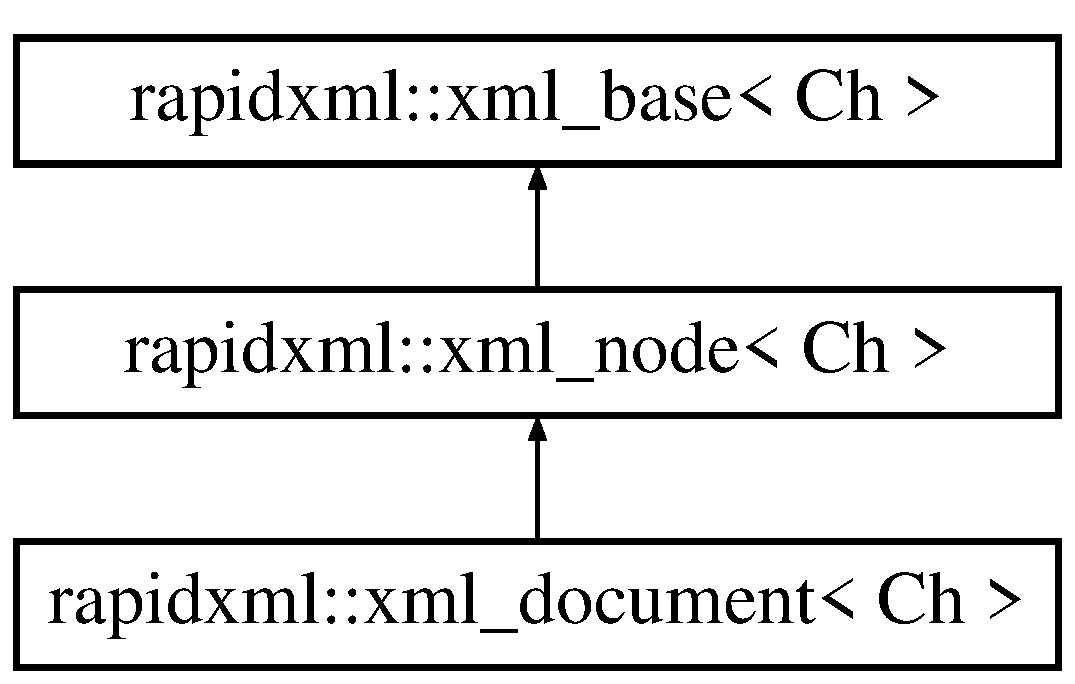
\includegraphics[height=3.000000cm]{classrapidxml_1_1xml__node}
\end{center}
\end{figure}
\subsection*{Public Member Functions}
\begin{DoxyCompactItemize}
\item 
\mbox{\hyperlink{classrapidxml_1_1xml__node_a8bd9019960b90605a45998b661fb1b0e}{xml\+\_\+node}} (\mbox{\hyperlink{rapidxml_8hpp_abb456db38f7efb746c4330eed6072a7c}{node\+\_\+type}} \mbox{\hyperlink{classrapidxml_1_1xml__node_a5f91729128856b0aaab598d4364ace60}{type}})
\item 
\mbox{\hyperlink{rapidxml_8hpp_abb456db38f7efb746c4330eed6072a7c}{node\+\_\+type}} \mbox{\hyperlink{classrapidxml_1_1xml__node_a5f91729128856b0aaab598d4364ace60}{type}} () const
\item 
\mbox{\hyperlink{classrapidxml_1_1xml__document}{xml\+\_\+document}}$<$ Ch $>$ $\ast$ \mbox{\hyperlink{classrapidxml_1_1xml__node_af23d2d56182411e9261ca6974bfd767f}{document}} () const
\item 
\mbox{\hyperlink{classrapidxml_1_1xml__node}{xml\+\_\+node}}$<$ Ch $>$ $\ast$ \mbox{\hyperlink{classrapidxml_1_1xml__node_acdf3691224d683f50692616a92a75d3f}{first\+\_\+node}} (const Ch $\ast$\mbox{\hyperlink{classrapidxml_1_1xml__base_aef8ae147fbee59209f714274afc80dc4}{name}}=0, std\+::size\+\_\+t \mbox{\hyperlink{classrapidxml_1_1xml__base_a20c8ffbe0c7a0b4231681ab8b99330a4}{name\+\_\+size}}=0, bool case\+\_\+sensitive=true) const
\item 
\mbox{\hyperlink{classrapidxml_1_1xml__node}{xml\+\_\+node}}$<$ Ch $>$ $\ast$ \mbox{\hyperlink{classrapidxml_1_1xml__node_a524d427e32c72fba9de1857e02e82fa7}{last\+\_\+node}} (const Ch $\ast$\mbox{\hyperlink{classrapidxml_1_1xml__base_aef8ae147fbee59209f714274afc80dc4}{name}}=0, std\+::size\+\_\+t \mbox{\hyperlink{classrapidxml_1_1xml__base_a20c8ffbe0c7a0b4231681ab8b99330a4}{name\+\_\+size}}=0, bool case\+\_\+sensitive=true) const
\item 
\mbox{\hyperlink{classrapidxml_1_1xml__node}{xml\+\_\+node}}$<$ Ch $>$ $\ast$ \mbox{\hyperlink{classrapidxml_1_1xml__node_aebcc42042ded78fb7020e2783f7d5426}{previous\+\_\+sibling}} (const Ch $\ast$\mbox{\hyperlink{classrapidxml_1_1xml__base_aef8ae147fbee59209f714274afc80dc4}{name}}=0, std\+::size\+\_\+t \mbox{\hyperlink{classrapidxml_1_1xml__base_a20c8ffbe0c7a0b4231681ab8b99330a4}{name\+\_\+size}}=0, bool case\+\_\+sensitive=true) const
\item 
\mbox{\hyperlink{classrapidxml_1_1xml__node}{xml\+\_\+node}}$<$ Ch $>$ $\ast$ \mbox{\hyperlink{classrapidxml_1_1xml__node_ad36aa4445ced578f93c3e06770cb3ef9}{next\+\_\+sibling}} (const Ch $\ast$\mbox{\hyperlink{classrapidxml_1_1xml__base_aef8ae147fbee59209f714274afc80dc4}{name}}=0, std\+::size\+\_\+t \mbox{\hyperlink{classrapidxml_1_1xml__base_a20c8ffbe0c7a0b4231681ab8b99330a4}{name\+\_\+size}}=0, bool case\+\_\+sensitive=true) const
\item 
\mbox{\hyperlink{classrapidxml_1_1xml__attribute}{xml\+\_\+attribute}}$<$ Ch $>$ $\ast$ \mbox{\hyperlink{classrapidxml_1_1xml__node_ab816ab6f13ee4b0588d5b76b0697511c}{first\+\_\+attribute}} (const Ch $\ast$\mbox{\hyperlink{classrapidxml_1_1xml__base_aef8ae147fbee59209f714274afc80dc4}{name}}=0, std\+::size\+\_\+t \mbox{\hyperlink{classrapidxml_1_1xml__base_a20c8ffbe0c7a0b4231681ab8b99330a4}{name\+\_\+size}}=0, bool case\+\_\+sensitive=true) const
\item 
\mbox{\hyperlink{classrapidxml_1_1xml__attribute}{xml\+\_\+attribute}}$<$ Ch $>$ $\ast$ \mbox{\hyperlink{classrapidxml_1_1xml__node_a67db03d1568dc6891573210ddba61520}{last\+\_\+attribute}} (const Ch $\ast$\mbox{\hyperlink{classrapidxml_1_1xml__base_aef8ae147fbee59209f714274afc80dc4}{name}}=0, std\+::size\+\_\+t \mbox{\hyperlink{classrapidxml_1_1xml__base_a20c8ffbe0c7a0b4231681ab8b99330a4}{name\+\_\+size}}=0, bool case\+\_\+sensitive=true) const
\item 
void \mbox{\hyperlink{classrapidxml_1_1xml__node_a499bbc9300c1b06821d5c08b24164c68}{type}} (\mbox{\hyperlink{rapidxml_8hpp_abb456db38f7efb746c4330eed6072a7c}{node\+\_\+type}} type)
\item 
void \mbox{\hyperlink{classrapidxml_1_1xml__node_ae86e92908c3eab40bbed8216e4f3f3cb}{prepend\+\_\+node}} (\mbox{\hyperlink{classrapidxml_1_1xml__node}{xml\+\_\+node}}$<$ Ch $>$ $\ast$child)
\item 
void \mbox{\hyperlink{classrapidxml_1_1xml__node_a8696d098ecc9c4d2a646b43e91d58e31}{append\+\_\+node}} (\mbox{\hyperlink{classrapidxml_1_1xml__node}{xml\+\_\+node}}$<$ Ch $>$ $\ast$child)
\item 
void \mbox{\hyperlink{classrapidxml_1_1xml__node_a666880f42a7e486d78cc45ed51c7c46d}{insert\+\_\+node}} (\mbox{\hyperlink{classrapidxml_1_1xml__node}{xml\+\_\+node}}$<$ Ch $>$ $\ast$where, \mbox{\hyperlink{classrapidxml_1_1xml__node}{xml\+\_\+node}}$<$ Ch $>$ $\ast$child)
\item 
void \mbox{\hyperlink{classrapidxml_1_1xml__node_a62bf7b276cf7a651a3337f5e0a0ef6ac}{remove\+\_\+first\+\_\+node}} ()
\item 
void \mbox{\hyperlink{classrapidxml_1_1xml__node_a9182512e948ec451a83f116cce7c7674}{remove\+\_\+last\+\_\+node}} ()
\item 
\mbox{\Hypertarget{classrapidxml_1_1xml__node_a98289923eb9e8889418a9eb0207ea35c}\label{classrapidxml_1_1xml__node_a98289923eb9e8889418a9eb0207ea35c}} 
void \mbox{\hyperlink{classrapidxml_1_1xml__node_a98289923eb9e8889418a9eb0207ea35c}{remove\+\_\+node}} (\mbox{\hyperlink{classrapidxml_1_1xml__node}{xml\+\_\+node}}$<$ Ch $>$ $\ast$where)
\begin{DoxyCompactList}\small\item\em Removes specified child from the node. \end{DoxyCompactList}\item 
\mbox{\Hypertarget{classrapidxml_1_1xml__node_a95735358b079ae0adcfbbac69aa1fbc3}\label{classrapidxml_1_1xml__node_a95735358b079ae0adcfbbac69aa1fbc3}} 
void \mbox{\hyperlink{classrapidxml_1_1xml__node_a95735358b079ae0adcfbbac69aa1fbc3}{remove\+\_\+all\+\_\+nodes}} ()
\begin{DoxyCompactList}\small\item\em Removes all child nodes (but not attributes). \end{DoxyCompactList}\item 
void \mbox{\hyperlink{classrapidxml_1_1xml__node_a8b62ee76489faf8e2d1210869d547684}{prepend\+\_\+attribute}} (\mbox{\hyperlink{classrapidxml_1_1xml__attribute}{xml\+\_\+attribute}}$<$ Ch $>$ $\ast$attribute)
\item 
void \mbox{\hyperlink{classrapidxml_1_1xml__node_a33ce3386f8c42dd4db658b75cbb6e6c4}{append\+\_\+attribute}} (\mbox{\hyperlink{classrapidxml_1_1xml__attribute}{xml\+\_\+attribute}}$<$ Ch $>$ $\ast$attribute)
\item 
void \mbox{\hyperlink{classrapidxml_1_1xml__node_a9fe659cdf4a5b3bbf5e8ffc98db5a84f}{insert\+\_\+attribute}} (\mbox{\hyperlink{classrapidxml_1_1xml__attribute}{xml\+\_\+attribute}}$<$ Ch $>$ $\ast$where, \mbox{\hyperlink{classrapidxml_1_1xml__attribute}{xml\+\_\+attribute}}$<$ Ch $>$ $\ast$attribute)
\item 
void \mbox{\hyperlink{classrapidxml_1_1xml__node_aa95192d2a165cca16c551ed2a2a06aec}{remove\+\_\+first\+\_\+attribute}} ()
\item 
void \mbox{\hyperlink{classrapidxml_1_1xml__node_a1781a2cbedc9a51d609ad5b528125635}{remove\+\_\+last\+\_\+attribute}} ()
\item 
void \mbox{\hyperlink{classrapidxml_1_1xml__node_a6f97b1b4f46a94a4587915df3c0c6b57}{remove\+\_\+attribute}} (\mbox{\hyperlink{classrapidxml_1_1xml__attribute}{xml\+\_\+attribute}}$<$ Ch $>$ $\ast$where)
\item 
\mbox{\Hypertarget{classrapidxml_1_1xml__node_aa8d5d9484aa1eb5ff1841a073c84c1aa}\label{classrapidxml_1_1xml__node_aa8d5d9484aa1eb5ff1841a073c84c1aa}} 
void \mbox{\hyperlink{classrapidxml_1_1xml__node_aa8d5d9484aa1eb5ff1841a073c84c1aa}{remove\+\_\+all\+\_\+attributes}} ()
\begin{DoxyCompactList}\small\item\em Removes all attributes of node. \end{DoxyCompactList}\end{DoxyCompactItemize}
\subsection*{Additional Inherited Members}


\subsection{Detailed Description}
\subsubsection*{template$<$class Ch = char$>$\newline
class rapidxml\+::xml\+\_\+node$<$ Ch $>$}

Class representing a node of X\+ML document. Each node may have associated name and value strings, which are available through \mbox{\hyperlink{classrapidxml_1_1xml__base_aef8ae147fbee59209f714274afc80dc4}{name()}} and \mbox{\hyperlink{classrapidxml_1_1xml__base_a6af65de5e59ac497cd69838f8a89d602}{value()}} functions. Interpretation of name and value depends on type of the node. Type of node can be determined by using \mbox{\hyperlink{classrapidxml_1_1xml__node_a5f91729128856b0aaab598d4364ace60}{type()}} function. ~\newline
~\newline
 Note that after parse, both name and value of node, if any, will point interior of source text used for parsing. Thus, this text must persist in the memory for the lifetime of node. 
\begin{DoxyParams}{Parameters}
{\em Ch} & Character type to use. \\
\hline
\end{DoxyParams}


\subsection{Constructor \& Destructor Documentation}
\mbox{\Hypertarget{classrapidxml_1_1xml__node_a8bd9019960b90605a45998b661fb1b0e}\label{classrapidxml_1_1xml__node_a8bd9019960b90605a45998b661fb1b0e}} 
\index{rapidxml\+::xml\+\_\+node@{rapidxml\+::xml\+\_\+node}!xml\+\_\+node@{xml\+\_\+node}}
\index{xml\+\_\+node@{xml\+\_\+node}!rapidxml\+::xml\+\_\+node@{rapidxml\+::xml\+\_\+node}}
\subsubsection{\texorpdfstring{xml\+\_\+node()}{xml\_node()}}
{\footnotesize\ttfamily template$<$class Ch = char$>$ \\
\mbox{\hyperlink{classrapidxml_1_1xml__node}{rapidxml\+::xml\+\_\+node}}$<$ Ch $>$\+::\mbox{\hyperlink{classrapidxml_1_1xml__node}{xml\+\_\+node}} (\begin{DoxyParamCaption}\item[{\mbox{\hyperlink{rapidxml_8hpp_abb456db38f7efb746c4330eed6072a7c}{node\+\_\+type}}}]{type }\end{DoxyParamCaption})\hspace{0.3cm}{\ttfamily [inline]}}

Constructs an empty node with the specified type. Consider using \mbox{\hyperlink{classrapidxml_1_1memory__pool}{memory\+\_\+pool}} of appropriate document to allocate nodes manually. 
\begin{DoxyParams}{Parameters}
{\em type} & Type of node to construct. \\
\hline
\end{DoxyParams}


\subsection{Member Function Documentation}
\mbox{\Hypertarget{classrapidxml_1_1xml__node_a33ce3386f8c42dd4db658b75cbb6e6c4}\label{classrapidxml_1_1xml__node_a33ce3386f8c42dd4db658b75cbb6e6c4}} 
\index{rapidxml\+::xml\+\_\+node@{rapidxml\+::xml\+\_\+node}!append\+\_\+attribute@{append\+\_\+attribute}}
\index{append\+\_\+attribute@{append\+\_\+attribute}!rapidxml\+::xml\+\_\+node@{rapidxml\+::xml\+\_\+node}}
\subsubsection{\texorpdfstring{append\+\_\+attribute()}{append\_attribute()}}
{\footnotesize\ttfamily template$<$class Ch = char$>$ \\
void \mbox{\hyperlink{classrapidxml_1_1xml__node}{rapidxml\+::xml\+\_\+node}}$<$ Ch $>$\+::append\+\_\+attribute (\begin{DoxyParamCaption}\item[{\mbox{\hyperlink{classrapidxml_1_1xml__attribute}{xml\+\_\+attribute}}$<$ Ch $>$ $\ast$}]{attribute }\end{DoxyParamCaption})\hspace{0.3cm}{\ttfamily [inline]}}

Appends a new attribute to the node. 
\begin{DoxyParams}{Parameters}
{\em attribute} & Attribute to append. \\
\hline
\end{DoxyParams}
\mbox{\Hypertarget{classrapidxml_1_1xml__node_a8696d098ecc9c4d2a646b43e91d58e31}\label{classrapidxml_1_1xml__node_a8696d098ecc9c4d2a646b43e91d58e31}} 
\index{rapidxml\+::xml\+\_\+node@{rapidxml\+::xml\+\_\+node}!append\+\_\+node@{append\+\_\+node}}
\index{append\+\_\+node@{append\+\_\+node}!rapidxml\+::xml\+\_\+node@{rapidxml\+::xml\+\_\+node}}
\subsubsection{\texorpdfstring{append\+\_\+node()}{append\_node()}}
{\footnotesize\ttfamily template$<$class Ch = char$>$ \\
void \mbox{\hyperlink{classrapidxml_1_1xml__node}{rapidxml\+::xml\+\_\+node}}$<$ Ch $>$\+::append\+\_\+node (\begin{DoxyParamCaption}\item[{\mbox{\hyperlink{classrapidxml_1_1xml__node}{xml\+\_\+node}}$<$ Ch $>$ $\ast$}]{child }\end{DoxyParamCaption})\hspace{0.3cm}{\ttfamily [inline]}}

Appends a new child node. The appended child becomes the last child. 
\begin{DoxyParams}{Parameters}
{\em child} & Node to append. \\
\hline
\end{DoxyParams}
\mbox{\Hypertarget{classrapidxml_1_1xml__node_af23d2d56182411e9261ca6974bfd767f}\label{classrapidxml_1_1xml__node_af23d2d56182411e9261ca6974bfd767f}} 
\index{rapidxml\+::xml\+\_\+node@{rapidxml\+::xml\+\_\+node}!document@{document}}
\index{document@{document}!rapidxml\+::xml\+\_\+node@{rapidxml\+::xml\+\_\+node}}
\subsubsection{\texorpdfstring{document()}{document()}}
{\footnotesize\ttfamily template$<$class Ch = char$>$ \\
\mbox{\hyperlink{classrapidxml_1_1xml__document}{xml\+\_\+document}}$<$Ch$>$$\ast$ \mbox{\hyperlink{classrapidxml_1_1xml__node}{rapidxml\+::xml\+\_\+node}}$<$ Ch $>$\+::document (\begin{DoxyParamCaption}{ }\end{DoxyParamCaption}) const\hspace{0.3cm}{\ttfamily [inline]}}

Gets document of which node is a child. \begin{DoxyReturn}{Returns}
Pointer to document that contains this node, or 0 if there is no parent document. 
\end{DoxyReturn}
\mbox{\Hypertarget{classrapidxml_1_1xml__node_ab816ab6f13ee4b0588d5b76b0697511c}\label{classrapidxml_1_1xml__node_ab816ab6f13ee4b0588d5b76b0697511c}} 
\index{rapidxml\+::xml\+\_\+node@{rapidxml\+::xml\+\_\+node}!first\+\_\+attribute@{first\+\_\+attribute}}
\index{first\+\_\+attribute@{first\+\_\+attribute}!rapidxml\+::xml\+\_\+node@{rapidxml\+::xml\+\_\+node}}
\subsubsection{\texorpdfstring{first\+\_\+attribute()}{first\_attribute()}}
{\footnotesize\ttfamily template$<$class Ch = char$>$ \\
\mbox{\hyperlink{classrapidxml_1_1xml__attribute}{xml\+\_\+attribute}}$<$Ch$>$$\ast$ \mbox{\hyperlink{classrapidxml_1_1xml__node}{rapidxml\+::xml\+\_\+node}}$<$ Ch $>$\+::first\+\_\+attribute (\begin{DoxyParamCaption}\item[{const Ch $\ast$}]{name = {\ttfamily 0},  }\item[{std\+::size\+\_\+t}]{name\+\_\+size = {\ttfamily 0},  }\item[{bool}]{case\+\_\+sensitive = {\ttfamily true} }\end{DoxyParamCaption}) const\hspace{0.3cm}{\ttfamily [inline]}}

Gets first attribute of node, optionally matching attribute name. 
\begin{DoxyParams}{Parameters}
{\em name} & Name of attribute to find, or 0 to return first attribute regardless of its name; this string doesn\textquotesingle{}t have to be zero-\/terminated if name\+\_\+size is non-\/zero \\
\hline
{\em name\+\_\+size} & Size of name, in characters, or 0 to have size calculated automatically from string \\
\hline
{\em case\+\_\+sensitive} & Should name comparison be case-\/sensitive; non case-\/sensitive comparison works properly only for A\+S\+C\+II characters \\
\hline
\end{DoxyParams}
\begin{DoxyReturn}{Returns}
Pointer to found attribute, or 0 if not found. 
\end{DoxyReturn}
\mbox{\Hypertarget{classrapidxml_1_1xml__node_acdf3691224d683f50692616a92a75d3f}\label{classrapidxml_1_1xml__node_acdf3691224d683f50692616a92a75d3f}} 
\index{rapidxml\+::xml\+\_\+node@{rapidxml\+::xml\+\_\+node}!first\+\_\+node@{first\+\_\+node}}
\index{first\+\_\+node@{first\+\_\+node}!rapidxml\+::xml\+\_\+node@{rapidxml\+::xml\+\_\+node}}
\subsubsection{\texorpdfstring{first\+\_\+node()}{first\_node()}}
{\footnotesize\ttfamily template$<$class Ch = char$>$ \\
\mbox{\hyperlink{classrapidxml_1_1xml__node}{xml\+\_\+node}}$<$Ch$>$$\ast$ \mbox{\hyperlink{classrapidxml_1_1xml__node}{rapidxml\+::xml\+\_\+node}}$<$ Ch $>$\+::first\+\_\+node (\begin{DoxyParamCaption}\item[{const Ch $\ast$}]{name = {\ttfamily 0},  }\item[{std\+::size\+\_\+t}]{name\+\_\+size = {\ttfamily 0},  }\item[{bool}]{case\+\_\+sensitive = {\ttfamily true} }\end{DoxyParamCaption}) const\hspace{0.3cm}{\ttfamily [inline]}}

Gets first child node, optionally matching node name. 
\begin{DoxyParams}{Parameters}
{\em name} & Name of child to find, or 0 to return first child regardless of its name; this string doesn\textquotesingle{}t have to be zero-\/terminated if name\+\_\+size is non-\/zero \\
\hline
{\em name\+\_\+size} & Size of name, in characters, or 0 to have size calculated automatically from string \\
\hline
{\em case\+\_\+sensitive} & Should name comparison be case-\/sensitive; non case-\/sensitive comparison works properly only for A\+S\+C\+II characters \\
\hline
\end{DoxyParams}
\begin{DoxyReturn}{Returns}
Pointer to found child, or 0 if not found. 
\end{DoxyReturn}
\mbox{\Hypertarget{classrapidxml_1_1xml__node_a9fe659cdf4a5b3bbf5e8ffc98db5a84f}\label{classrapidxml_1_1xml__node_a9fe659cdf4a5b3bbf5e8ffc98db5a84f}} 
\index{rapidxml\+::xml\+\_\+node@{rapidxml\+::xml\+\_\+node}!insert\+\_\+attribute@{insert\+\_\+attribute}}
\index{insert\+\_\+attribute@{insert\+\_\+attribute}!rapidxml\+::xml\+\_\+node@{rapidxml\+::xml\+\_\+node}}
\subsubsection{\texorpdfstring{insert\+\_\+attribute()}{insert\_attribute()}}
{\footnotesize\ttfamily template$<$class Ch = char$>$ \\
void \mbox{\hyperlink{classrapidxml_1_1xml__node}{rapidxml\+::xml\+\_\+node}}$<$ Ch $>$\+::insert\+\_\+attribute (\begin{DoxyParamCaption}\item[{\mbox{\hyperlink{classrapidxml_1_1xml__attribute}{xml\+\_\+attribute}}$<$ Ch $>$ $\ast$}]{where,  }\item[{\mbox{\hyperlink{classrapidxml_1_1xml__attribute}{xml\+\_\+attribute}}$<$ Ch $>$ $\ast$}]{attribute }\end{DoxyParamCaption})\hspace{0.3cm}{\ttfamily [inline]}}

Inserts a new attribute at specified place inside the node. All attributes after and including the specified attribute are moved one position back. 
\begin{DoxyParams}{Parameters}
{\em where} & Place where to insert the attribute, or 0 to insert at the back. \\
\hline
{\em attribute} & Attribute to insert. \\
\hline
\end{DoxyParams}
\mbox{\Hypertarget{classrapidxml_1_1xml__node_a666880f42a7e486d78cc45ed51c7c46d}\label{classrapidxml_1_1xml__node_a666880f42a7e486d78cc45ed51c7c46d}} 
\index{rapidxml\+::xml\+\_\+node@{rapidxml\+::xml\+\_\+node}!insert\+\_\+node@{insert\+\_\+node}}
\index{insert\+\_\+node@{insert\+\_\+node}!rapidxml\+::xml\+\_\+node@{rapidxml\+::xml\+\_\+node}}
\subsubsection{\texorpdfstring{insert\+\_\+node()}{insert\_node()}}
{\footnotesize\ttfamily template$<$class Ch = char$>$ \\
void \mbox{\hyperlink{classrapidxml_1_1xml__node}{rapidxml\+::xml\+\_\+node}}$<$ Ch $>$\+::insert\+\_\+node (\begin{DoxyParamCaption}\item[{\mbox{\hyperlink{classrapidxml_1_1xml__node}{xml\+\_\+node}}$<$ Ch $>$ $\ast$}]{where,  }\item[{\mbox{\hyperlink{classrapidxml_1_1xml__node}{xml\+\_\+node}}$<$ Ch $>$ $\ast$}]{child }\end{DoxyParamCaption})\hspace{0.3cm}{\ttfamily [inline]}}

Inserts a new child node at specified place inside the node. All children after and including the specified node are moved one position back. 
\begin{DoxyParams}{Parameters}
{\em where} & Place where to insert the child, or 0 to insert at the back. \\
\hline
{\em child} & Node to insert. \\
\hline
\end{DoxyParams}
\mbox{\Hypertarget{classrapidxml_1_1xml__node_a67db03d1568dc6891573210ddba61520}\label{classrapidxml_1_1xml__node_a67db03d1568dc6891573210ddba61520}} 
\index{rapidxml\+::xml\+\_\+node@{rapidxml\+::xml\+\_\+node}!last\+\_\+attribute@{last\+\_\+attribute}}
\index{last\+\_\+attribute@{last\+\_\+attribute}!rapidxml\+::xml\+\_\+node@{rapidxml\+::xml\+\_\+node}}
\subsubsection{\texorpdfstring{last\+\_\+attribute()}{last\_attribute()}}
{\footnotesize\ttfamily template$<$class Ch = char$>$ \\
\mbox{\hyperlink{classrapidxml_1_1xml__attribute}{xml\+\_\+attribute}}$<$Ch$>$$\ast$ \mbox{\hyperlink{classrapidxml_1_1xml__node}{rapidxml\+::xml\+\_\+node}}$<$ Ch $>$\+::last\+\_\+attribute (\begin{DoxyParamCaption}\item[{const Ch $\ast$}]{name = {\ttfamily 0},  }\item[{std\+::size\+\_\+t}]{name\+\_\+size = {\ttfamily 0},  }\item[{bool}]{case\+\_\+sensitive = {\ttfamily true} }\end{DoxyParamCaption}) const\hspace{0.3cm}{\ttfamily [inline]}}

Gets last attribute of node, optionally matching attribute name. 
\begin{DoxyParams}{Parameters}
{\em name} & Name of attribute to find, or 0 to return last attribute regardless of its name; this string doesn\textquotesingle{}t have to be zero-\/terminated if name\+\_\+size is non-\/zero \\
\hline
{\em name\+\_\+size} & Size of name, in characters, or 0 to have size calculated automatically from string \\
\hline
{\em case\+\_\+sensitive} & Should name comparison be case-\/sensitive; non case-\/sensitive comparison works properly only for A\+S\+C\+II characters \\
\hline
\end{DoxyParams}
\begin{DoxyReturn}{Returns}
Pointer to found attribute, or 0 if not found. 
\end{DoxyReturn}
\mbox{\Hypertarget{classrapidxml_1_1xml__node_a524d427e32c72fba9de1857e02e82fa7}\label{classrapidxml_1_1xml__node_a524d427e32c72fba9de1857e02e82fa7}} 
\index{rapidxml\+::xml\+\_\+node@{rapidxml\+::xml\+\_\+node}!last\+\_\+node@{last\+\_\+node}}
\index{last\+\_\+node@{last\+\_\+node}!rapidxml\+::xml\+\_\+node@{rapidxml\+::xml\+\_\+node}}
\subsubsection{\texorpdfstring{last\+\_\+node()}{last\_node()}}
{\footnotesize\ttfamily template$<$class Ch = char$>$ \\
\mbox{\hyperlink{classrapidxml_1_1xml__node}{xml\+\_\+node}}$<$Ch$>$$\ast$ \mbox{\hyperlink{classrapidxml_1_1xml__node}{rapidxml\+::xml\+\_\+node}}$<$ Ch $>$\+::last\+\_\+node (\begin{DoxyParamCaption}\item[{const Ch $\ast$}]{name = {\ttfamily 0},  }\item[{std\+::size\+\_\+t}]{name\+\_\+size = {\ttfamily 0},  }\item[{bool}]{case\+\_\+sensitive = {\ttfamily true} }\end{DoxyParamCaption}) const\hspace{0.3cm}{\ttfamily [inline]}}

Gets last child node, optionally matching node name. Behaviour is undefined if node has no children. Use \mbox{\hyperlink{classrapidxml_1_1xml__node_acdf3691224d683f50692616a92a75d3f}{first\+\_\+node()}} to test if node has children. 
\begin{DoxyParams}{Parameters}
{\em name} & Name of child to find, or 0 to return last child regardless of its name; this string doesn\textquotesingle{}t have to be zero-\/terminated if name\+\_\+size is non-\/zero \\
\hline
{\em name\+\_\+size} & Size of name, in characters, or 0 to have size calculated automatically from string \\
\hline
{\em case\+\_\+sensitive} & Should name comparison be case-\/sensitive; non case-\/sensitive comparison works properly only for A\+S\+C\+II characters \\
\hline
\end{DoxyParams}
\begin{DoxyReturn}{Returns}
Pointer to found child, or 0 if not found. 
\end{DoxyReturn}
\mbox{\Hypertarget{classrapidxml_1_1xml__node_ad36aa4445ced578f93c3e06770cb3ef9}\label{classrapidxml_1_1xml__node_ad36aa4445ced578f93c3e06770cb3ef9}} 
\index{rapidxml\+::xml\+\_\+node@{rapidxml\+::xml\+\_\+node}!next\+\_\+sibling@{next\+\_\+sibling}}
\index{next\+\_\+sibling@{next\+\_\+sibling}!rapidxml\+::xml\+\_\+node@{rapidxml\+::xml\+\_\+node}}
\subsubsection{\texorpdfstring{next\+\_\+sibling()}{next\_sibling()}}
{\footnotesize\ttfamily template$<$class Ch = char$>$ \\
\mbox{\hyperlink{classrapidxml_1_1xml__node}{xml\+\_\+node}}$<$Ch$>$$\ast$ \mbox{\hyperlink{classrapidxml_1_1xml__node}{rapidxml\+::xml\+\_\+node}}$<$ Ch $>$\+::next\+\_\+sibling (\begin{DoxyParamCaption}\item[{const Ch $\ast$}]{name = {\ttfamily 0},  }\item[{std\+::size\+\_\+t}]{name\+\_\+size = {\ttfamily 0},  }\item[{bool}]{case\+\_\+sensitive = {\ttfamily true} }\end{DoxyParamCaption}) const\hspace{0.3cm}{\ttfamily [inline]}}

Gets next sibling node, optionally matching node name. Behaviour is undefined if node has no parent. Use \mbox{\hyperlink{classrapidxml_1_1xml__base_aa807062868d671a8c798d9d1bf016988}{parent()}} to test if node has a parent. 
\begin{DoxyParams}{Parameters}
{\em name} & Name of sibling to find, or 0 to return next sibling regardless of its name; this string doesn\textquotesingle{}t have to be zero-\/terminated if name\+\_\+size is non-\/zero \\
\hline
{\em name\+\_\+size} & Size of name, in characters, or 0 to have size calculated automatically from string \\
\hline
{\em case\+\_\+sensitive} & Should name comparison be case-\/sensitive; non case-\/sensitive comparison works properly only for A\+S\+C\+II characters \\
\hline
\end{DoxyParams}
\begin{DoxyReturn}{Returns}
Pointer to found sibling, or 0 if not found. 
\end{DoxyReturn}
\mbox{\Hypertarget{classrapidxml_1_1xml__node_a8b62ee76489faf8e2d1210869d547684}\label{classrapidxml_1_1xml__node_a8b62ee76489faf8e2d1210869d547684}} 
\index{rapidxml\+::xml\+\_\+node@{rapidxml\+::xml\+\_\+node}!prepend\+\_\+attribute@{prepend\+\_\+attribute}}
\index{prepend\+\_\+attribute@{prepend\+\_\+attribute}!rapidxml\+::xml\+\_\+node@{rapidxml\+::xml\+\_\+node}}
\subsubsection{\texorpdfstring{prepend\+\_\+attribute()}{prepend\_attribute()}}
{\footnotesize\ttfamily template$<$class Ch = char$>$ \\
void \mbox{\hyperlink{classrapidxml_1_1xml__node}{rapidxml\+::xml\+\_\+node}}$<$ Ch $>$\+::prepend\+\_\+attribute (\begin{DoxyParamCaption}\item[{\mbox{\hyperlink{classrapidxml_1_1xml__attribute}{xml\+\_\+attribute}}$<$ Ch $>$ $\ast$}]{attribute }\end{DoxyParamCaption})\hspace{0.3cm}{\ttfamily [inline]}}

Prepends a new attribute to the node. 
\begin{DoxyParams}{Parameters}
{\em attribute} & Attribute to prepend. \\
\hline
\end{DoxyParams}
\mbox{\Hypertarget{classrapidxml_1_1xml__node_ae86e92908c3eab40bbed8216e4f3f3cb}\label{classrapidxml_1_1xml__node_ae86e92908c3eab40bbed8216e4f3f3cb}} 
\index{rapidxml\+::xml\+\_\+node@{rapidxml\+::xml\+\_\+node}!prepend\+\_\+node@{prepend\+\_\+node}}
\index{prepend\+\_\+node@{prepend\+\_\+node}!rapidxml\+::xml\+\_\+node@{rapidxml\+::xml\+\_\+node}}
\subsubsection{\texorpdfstring{prepend\+\_\+node()}{prepend\_node()}}
{\footnotesize\ttfamily template$<$class Ch = char$>$ \\
void \mbox{\hyperlink{classrapidxml_1_1xml__node}{rapidxml\+::xml\+\_\+node}}$<$ Ch $>$\+::prepend\+\_\+node (\begin{DoxyParamCaption}\item[{\mbox{\hyperlink{classrapidxml_1_1xml__node}{xml\+\_\+node}}$<$ Ch $>$ $\ast$}]{child }\end{DoxyParamCaption})\hspace{0.3cm}{\ttfamily [inline]}}

Prepends a new child node. The prepended child becomes the first child, and all existing children are moved one position back. 
\begin{DoxyParams}{Parameters}
{\em child} & Node to prepend. \\
\hline
\end{DoxyParams}
\mbox{\Hypertarget{classrapidxml_1_1xml__node_aebcc42042ded78fb7020e2783f7d5426}\label{classrapidxml_1_1xml__node_aebcc42042ded78fb7020e2783f7d5426}} 
\index{rapidxml\+::xml\+\_\+node@{rapidxml\+::xml\+\_\+node}!previous\+\_\+sibling@{previous\+\_\+sibling}}
\index{previous\+\_\+sibling@{previous\+\_\+sibling}!rapidxml\+::xml\+\_\+node@{rapidxml\+::xml\+\_\+node}}
\subsubsection{\texorpdfstring{previous\+\_\+sibling()}{previous\_sibling()}}
{\footnotesize\ttfamily template$<$class Ch = char$>$ \\
\mbox{\hyperlink{classrapidxml_1_1xml__node}{xml\+\_\+node}}$<$Ch$>$$\ast$ \mbox{\hyperlink{classrapidxml_1_1xml__node}{rapidxml\+::xml\+\_\+node}}$<$ Ch $>$\+::previous\+\_\+sibling (\begin{DoxyParamCaption}\item[{const Ch $\ast$}]{name = {\ttfamily 0},  }\item[{std\+::size\+\_\+t}]{name\+\_\+size = {\ttfamily 0},  }\item[{bool}]{case\+\_\+sensitive = {\ttfamily true} }\end{DoxyParamCaption}) const\hspace{0.3cm}{\ttfamily [inline]}}

Gets previous sibling node, optionally matching node name. Behaviour is undefined if node has no parent. Use \mbox{\hyperlink{classrapidxml_1_1xml__base_aa807062868d671a8c798d9d1bf016988}{parent()}} to test if node has a parent. 
\begin{DoxyParams}{Parameters}
{\em name} & Name of sibling to find, or 0 to return previous sibling regardless of its name; this string doesn\textquotesingle{}t have to be zero-\/terminated if name\+\_\+size is non-\/zero \\
\hline
{\em name\+\_\+size} & Size of name, in characters, or 0 to have size calculated automatically from string \\
\hline
{\em case\+\_\+sensitive} & Should name comparison be case-\/sensitive; non case-\/sensitive comparison works properly only for A\+S\+C\+II characters \\
\hline
\end{DoxyParams}
\begin{DoxyReturn}{Returns}
Pointer to found sibling, or 0 if not found. 
\end{DoxyReturn}
\mbox{\Hypertarget{classrapidxml_1_1xml__node_a6f97b1b4f46a94a4587915df3c0c6b57}\label{classrapidxml_1_1xml__node_a6f97b1b4f46a94a4587915df3c0c6b57}} 
\index{rapidxml\+::xml\+\_\+node@{rapidxml\+::xml\+\_\+node}!remove\+\_\+attribute@{remove\+\_\+attribute}}
\index{remove\+\_\+attribute@{remove\+\_\+attribute}!rapidxml\+::xml\+\_\+node@{rapidxml\+::xml\+\_\+node}}
\subsubsection{\texorpdfstring{remove\+\_\+attribute()}{remove\_attribute()}}
{\footnotesize\ttfamily template$<$class Ch = char$>$ \\
void \mbox{\hyperlink{classrapidxml_1_1xml__node}{rapidxml\+::xml\+\_\+node}}$<$ Ch $>$\+::remove\+\_\+attribute (\begin{DoxyParamCaption}\item[{\mbox{\hyperlink{classrapidxml_1_1xml__attribute}{xml\+\_\+attribute}}$<$ Ch $>$ $\ast$}]{where }\end{DoxyParamCaption})\hspace{0.3cm}{\ttfamily [inline]}}

Removes specified attribute from node. 
\begin{DoxyParams}{Parameters}
{\em where} & Pointer to attribute to be removed. \\
\hline
\end{DoxyParams}
\mbox{\Hypertarget{classrapidxml_1_1xml__node_aa95192d2a165cca16c551ed2a2a06aec}\label{classrapidxml_1_1xml__node_aa95192d2a165cca16c551ed2a2a06aec}} 
\index{rapidxml\+::xml\+\_\+node@{rapidxml\+::xml\+\_\+node}!remove\+\_\+first\+\_\+attribute@{remove\+\_\+first\+\_\+attribute}}
\index{remove\+\_\+first\+\_\+attribute@{remove\+\_\+first\+\_\+attribute}!rapidxml\+::xml\+\_\+node@{rapidxml\+::xml\+\_\+node}}
\subsubsection{\texorpdfstring{remove\+\_\+first\+\_\+attribute()}{remove\_first\_attribute()}}
{\footnotesize\ttfamily template$<$class Ch = char$>$ \\
void \mbox{\hyperlink{classrapidxml_1_1xml__node}{rapidxml\+::xml\+\_\+node}}$<$ Ch $>$\+::remove\+\_\+first\+\_\+attribute (\begin{DoxyParamCaption}{ }\end{DoxyParamCaption})\hspace{0.3cm}{\ttfamily [inline]}}

Removes first attribute of the node. If node has no attributes, behaviour is undefined. Use \mbox{\hyperlink{classrapidxml_1_1xml__node_ab816ab6f13ee4b0588d5b76b0697511c}{first\+\_\+attribute()}} to test if node has attributes. \mbox{\Hypertarget{classrapidxml_1_1xml__node_a62bf7b276cf7a651a3337f5e0a0ef6ac}\label{classrapidxml_1_1xml__node_a62bf7b276cf7a651a3337f5e0a0ef6ac}} 
\index{rapidxml\+::xml\+\_\+node@{rapidxml\+::xml\+\_\+node}!remove\+\_\+first\+\_\+node@{remove\+\_\+first\+\_\+node}}
\index{remove\+\_\+first\+\_\+node@{remove\+\_\+first\+\_\+node}!rapidxml\+::xml\+\_\+node@{rapidxml\+::xml\+\_\+node}}
\subsubsection{\texorpdfstring{remove\+\_\+first\+\_\+node()}{remove\_first\_node()}}
{\footnotesize\ttfamily template$<$class Ch = char$>$ \\
void \mbox{\hyperlink{classrapidxml_1_1xml__node}{rapidxml\+::xml\+\_\+node}}$<$ Ch $>$\+::remove\+\_\+first\+\_\+node (\begin{DoxyParamCaption}{ }\end{DoxyParamCaption})\hspace{0.3cm}{\ttfamily [inline]}}

Removes first child node. If node has no children, behaviour is undefined. Use \mbox{\hyperlink{classrapidxml_1_1xml__node_acdf3691224d683f50692616a92a75d3f}{first\+\_\+node()}} to test if node has children. \mbox{\Hypertarget{classrapidxml_1_1xml__node_a1781a2cbedc9a51d609ad5b528125635}\label{classrapidxml_1_1xml__node_a1781a2cbedc9a51d609ad5b528125635}} 
\index{rapidxml\+::xml\+\_\+node@{rapidxml\+::xml\+\_\+node}!remove\+\_\+last\+\_\+attribute@{remove\+\_\+last\+\_\+attribute}}
\index{remove\+\_\+last\+\_\+attribute@{remove\+\_\+last\+\_\+attribute}!rapidxml\+::xml\+\_\+node@{rapidxml\+::xml\+\_\+node}}
\subsubsection{\texorpdfstring{remove\+\_\+last\+\_\+attribute()}{remove\_last\_attribute()}}
{\footnotesize\ttfamily template$<$class Ch = char$>$ \\
void \mbox{\hyperlink{classrapidxml_1_1xml__node}{rapidxml\+::xml\+\_\+node}}$<$ Ch $>$\+::remove\+\_\+last\+\_\+attribute (\begin{DoxyParamCaption}{ }\end{DoxyParamCaption})\hspace{0.3cm}{\ttfamily [inline]}}

Removes last attribute of the node. If node has no attributes, behaviour is undefined. Use \mbox{\hyperlink{classrapidxml_1_1xml__node_ab816ab6f13ee4b0588d5b76b0697511c}{first\+\_\+attribute()}} to test if node has attributes. \mbox{\Hypertarget{classrapidxml_1_1xml__node_a9182512e948ec451a83f116cce7c7674}\label{classrapidxml_1_1xml__node_a9182512e948ec451a83f116cce7c7674}} 
\index{rapidxml\+::xml\+\_\+node@{rapidxml\+::xml\+\_\+node}!remove\+\_\+last\+\_\+node@{remove\+\_\+last\+\_\+node}}
\index{remove\+\_\+last\+\_\+node@{remove\+\_\+last\+\_\+node}!rapidxml\+::xml\+\_\+node@{rapidxml\+::xml\+\_\+node}}
\subsubsection{\texorpdfstring{remove\+\_\+last\+\_\+node()}{remove\_last\_node()}}
{\footnotesize\ttfamily template$<$class Ch = char$>$ \\
void \mbox{\hyperlink{classrapidxml_1_1xml__node}{rapidxml\+::xml\+\_\+node}}$<$ Ch $>$\+::remove\+\_\+last\+\_\+node (\begin{DoxyParamCaption}{ }\end{DoxyParamCaption})\hspace{0.3cm}{\ttfamily [inline]}}

Removes last child of the node. If node has no children, behaviour is undefined. Use \mbox{\hyperlink{classrapidxml_1_1xml__node_acdf3691224d683f50692616a92a75d3f}{first\+\_\+node()}} to test if node has children. \mbox{\Hypertarget{classrapidxml_1_1xml__node_a5f91729128856b0aaab598d4364ace60}\label{classrapidxml_1_1xml__node_a5f91729128856b0aaab598d4364ace60}} 
\index{rapidxml\+::xml\+\_\+node@{rapidxml\+::xml\+\_\+node}!type@{type}}
\index{type@{type}!rapidxml\+::xml\+\_\+node@{rapidxml\+::xml\+\_\+node}}
\subsubsection{\texorpdfstring{type()}{type()}\hspace{0.1cm}{\footnotesize\ttfamily [1/2]}}
{\footnotesize\ttfamily template$<$class Ch = char$>$ \\
\mbox{\hyperlink{rapidxml_8hpp_abb456db38f7efb746c4330eed6072a7c}{node\+\_\+type}} \mbox{\hyperlink{classrapidxml_1_1xml__node}{rapidxml\+::xml\+\_\+node}}$<$ Ch $>$\+::type (\begin{DoxyParamCaption}{ }\end{DoxyParamCaption}) const\hspace{0.3cm}{\ttfamily [inline]}}

Gets type of node. \begin{DoxyReturn}{Returns}
Type of node. 
\end{DoxyReturn}
\mbox{\Hypertarget{classrapidxml_1_1xml__node_a499bbc9300c1b06821d5c08b24164c68}\label{classrapidxml_1_1xml__node_a499bbc9300c1b06821d5c08b24164c68}} 
\index{rapidxml\+::xml\+\_\+node@{rapidxml\+::xml\+\_\+node}!type@{type}}
\index{type@{type}!rapidxml\+::xml\+\_\+node@{rapidxml\+::xml\+\_\+node}}
\subsubsection{\texorpdfstring{type()}{type()}\hspace{0.1cm}{\footnotesize\ttfamily [2/2]}}
{\footnotesize\ttfamily template$<$class Ch = char$>$ \\
void \mbox{\hyperlink{classrapidxml_1_1xml__node}{rapidxml\+::xml\+\_\+node}}$<$ Ch $>$\+::type (\begin{DoxyParamCaption}\item[{\mbox{\hyperlink{rapidxml_8hpp_abb456db38f7efb746c4330eed6072a7c}{node\+\_\+type}}}]{type }\end{DoxyParamCaption})\hspace{0.3cm}{\ttfamily [inline]}}

Sets type of node. 
\begin{DoxyParams}{Parameters}
{\em type} & Type of node to set. \\
\hline
\end{DoxyParams}


The documentation for this class was generated from the following file\+:\begin{DoxyCompactItemize}
\item 
Tower\+Defence/\+Graphics\+Handler/\mbox{\hyperlink{rapidxml_8hpp}{rapidxml.\+hpp}}\end{DoxyCompactItemize}

\hypertarget{class_zombie}{}\section{Zombie Class Reference}
\label{class_zombie}\index{Zombie@{Zombie}}


Class representing zombie.  




{\ttfamily \#include $<$Enemy\+Designer.\+h$>$}

Inheritance diagram for Zombie\+:\begin{figure}[H]
\begin{center}
\leavevmode
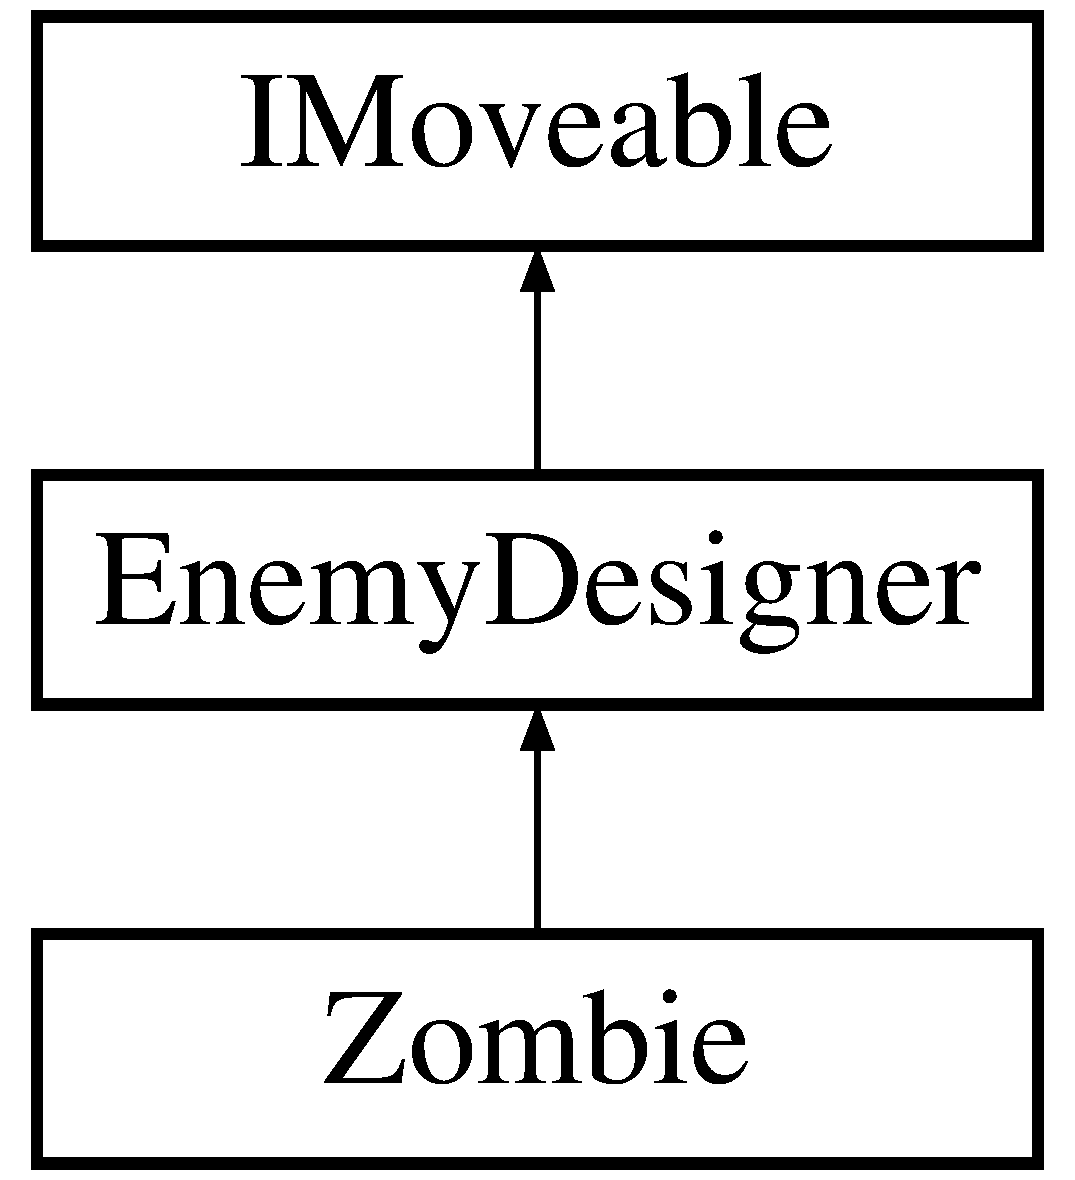
\includegraphics[height=3.000000cm]{class_zombie}
\end{center}
\end{figure}
\subsection*{Public Member Functions}
\begin{DoxyCompactItemize}
\item 
\mbox{\hyperlink{class_zombie_ae090d581d9788f7cd13a474f6f3f2667}{Zombie}} (sf\+::\+Vector2f origin, sf\+::\+Vector2f dimensions, sf\+::\+Color color, sf\+::\+Vector2f texture\+Dimensions, std\+::string=\char`\"{}zombie.\+png\char`\"{})
\begin{DoxyCompactList}\small\item\em constructor for zombie class \end{DoxyCompactList}\end{DoxyCompactItemize}
\subsection*{Additional Inherited Members}


\subsection{Detailed Description}
Class representing zombie. 

\subsection{Constructor \& Destructor Documentation}
\mbox{\Hypertarget{class_zombie_ae090d581d9788f7cd13a474f6f3f2667}\label{class_zombie_ae090d581d9788f7cd13a474f6f3f2667}} 
\index{Zombie@{Zombie}!Zombie@{Zombie}}
\index{Zombie@{Zombie}!Zombie@{Zombie}}
\subsubsection{\texorpdfstring{Zombie()}{Zombie()}}
{\footnotesize\ttfamily Zombie\+::\+Zombie (\begin{DoxyParamCaption}\item[{sf\+::\+Vector2f}]{origin,  }\item[{sf\+::\+Vector2f}]{dimensions,  }\item[{sf\+::\+Color}]{color,  }\item[{sf\+::\+Vector2f}]{texture\+Dimensions,  }\item[{std\+::string}]{texture\+File = {\ttfamily \char`\"{}zombie.png\char`\"{}} }\end{DoxyParamCaption})}



constructor for zombie class 


\begin{DoxyParams}{Parameters}
{\em origin} & point \\
\hline
{\em dimensions} & \\
\hline
{\em color} & \\
\hline
{\em texture} & dimensions \\
\hline
{\em file} & containing texture \\
\hline
\end{DoxyParams}


The documentation for this class was generated from the following files\+:\begin{DoxyCompactItemize}
\item 
Tower\+Defence/\+Graphics\+Handler/Enemy\+Designer.\+h\item 
Tower\+Defence/\+Graphics\+Handler/Enemy\+Designer.\+cpp\end{DoxyCompactItemize}

\chapter{File Documentation}
\hypertarget{rapidxml_8hpp}{}\section{Tower\+Defence/\+Graphics\+Handler/rapidxml.hpp File Reference}
\label{rapidxml_8hpp}\index{Tower\+Defence/\+Graphics\+Handler/rapidxml.\+hpp@{Tower\+Defence/\+Graphics\+Handler/rapidxml.\+hpp}}


This file contains rapidxml parser and D\+OM implementation.  


{\ttfamily \#include $<$cstdlib$>$}\newline
{\ttfamily \#include $<$cassert$>$}\newline
{\ttfamily \#include $<$new$>$}\newline
{\ttfamily \#include $<$exception$>$}\newline
\subsection*{Classes}
\begin{DoxyCompactItemize}
\item 
class \mbox{\hyperlink{classrapidxml_1_1parse__error}{rapidxml\+::parse\+\_\+error}}
\item 
class \mbox{\hyperlink{classrapidxml_1_1xml__node}{rapidxml\+::xml\+\_\+node$<$ Ch $>$}}
\item 
class \mbox{\hyperlink{classrapidxml_1_1xml__attribute}{rapidxml\+::xml\+\_\+attribute$<$ Ch $>$}}
\item 
class \mbox{\hyperlink{classrapidxml_1_1xml__document}{rapidxml\+::xml\+\_\+document$<$ Ch $>$}}
\item 
class \mbox{\hyperlink{classrapidxml_1_1memory__pool}{rapidxml\+::memory\+\_\+pool$<$ Ch $>$}}
\item 
class \mbox{\hyperlink{classrapidxml_1_1xml__base}{rapidxml\+::xml\+\_\+base$<$ Ch $>$}}
\item 
class \mbox{\hyperlink{classrapidxml_1_1xml__attribute}{rapidxml\+::xml\+\_\+attribute$<$ Ch $>$}}
\item 
class \mbox{\hyperlink{classrapidxml_1_1xml__node}{rapidxml\+::xml\+\_\+node$<$ Ch $>$}}
\item 
class \mbox{\hyperlink{classrapidxml_1_1xml__document}{rapidxml\+::xml\+\_\+document$<$ Ch $>$}}
\end{DoxyCompactItemize}
\subsection*{Macros}
\begin{DoxyCompactItemize}
\item 
\mbox{\Hypertarget{rapidxml_8hpp_a65f2be309896ffb841997d467c2f4fff}\label{rapidxml_8hpp_a65f2be309896ffb841997d467c2f4fff}} 
\#define {\bfseries R\+A\+P\+I\+D\+X\+M\+L\+\_\+\+P\+A\+R\+S\+E\+\_\+\+E\+R\+R\+OR}(what,  where)~throw parse\+\_\+error(what, where)
\item 
\mbox{\Hypertarget{rapidxml_8hpp_a001304844ab478e3b213749fc8d72ca2}\label{rapidxml_8hpp_a001304844ab478e3b213749fc8d72ca2}} 
\#define {\bfseries R\+A\+P\+I\+D\+X\+M\+L\+\_\+\+S\+T\+A\+T\+I\+C\+\_\+\+P\+O\+O\+L\+\_\+\+S\+I\+ZE}~(64 $\ast$ 1024)
\item 
\mbox{\Hypertarget{rapidxml_8hpp_a68d5603b71691d9dd745e45159259aa3}\label{rapidxml_8hpp_a68d5603b71691d9dd745e45159259aa3}} 
\#define {\bfseries R\+A\+P\+I\+D\+X\+M\+L\+\_\+\+D\+Y\+N\+A\+M\+I\+C\+\_\+\+P\+O\+O\+L\+\_\+\+S\+I\+ZE}~(64 $\ast$ 1024)
\item 
\mbox{\Hypertarget{rapidxml_8hpp_ad3344fdba5167e17f48a8b2318731198}\label{rapidxml_8hpp_ad3344fdba5167e17f48a8b2318731198}} 
\#define {\bfseries R\+A\+P\+I\+D\+X\+M\+L\+\_\+\+A\+L\+I\+G\+N\+M\+E\+NT}~sizeof(void $\ast$)
\end{DoxyCompactItemize}
\subsection*{Enumerations}
\begin{DoxyCompactItemize}
\item 
enum \mbox{\hyperlink{rapidxml_8hpp_abb456db38f7efb746c4330eed6072a7c}{rapidxml\+::node\+\_\+type}} \{ \newline
\mbox{\hyperlink{rapidxml_8hpp_abb456db38f7efb746c4330eed6072a7ca4023b6a1c7059fd8fbec2112d5c35424}{rapidxml\+::node\+\_\+document}}, 
\mbox{\hyperlink{rapidxml_8hpp_abb456db38f7efb746c4330eed6072a7ca89cbeb4d28046326e4ee953d3c4047ff}{rapidxml\+::node\+\_\+element}}, 
\mbox{\hyperlink{rapidxml_8hpp_abb456db38f7efb746c4330eed6072a7ca9d669d8e1f4ba9c7eeada4c14a11ad1d}{rapidxml\+::node\+\_\+data}}, 
\mbox{\hyperlink{rapidxml_8hpp_abb456db38f7efb746c4330eed6072a7caccf0b363d3876a3f83ff9b1bcdaaa536}{rapidxml\+::node\+\_\+cdata}}, 
\newline
\mbox{\hyperlink{rapidxml_8hpp_abb456db38f7efb746c4330eed6072a7ca1a695e1384ec3bd4df3eff65ec609a96}{rapidxml\+::node\+\_\+comment}}, 
\mbox{\hyperlink{rapidxml_8hpp_abb456db38f7efb746c4330eed6072a7cafe4ca44261e5fbedf0eab43131751212}{rapidxml\+::node\+\_\+declaration}}, 
\mbox{\hyperlink{rapidxml_8hpp_abb456db38f7efb746c4330eed6072a7cadf5002f2efabe231bed01d16f08f832c}{rapidxml\+::node\+\_\+doctype}}, 
\mbox{\hyperlink{rapidxml_8hpp_abb456db38f7efb746c4330eed6072a7caeb73b472e77347b9aa89525f16493b87}{rapidxml\+::node\+\_\+pi}}
 \}
\end{DoxyCompactItemize}
\subsection*{Variables}
\begin{DoxyCompactItemize}
\item 
const int \mbox{\hyperlink{rapidxml_8hpp_ac2d21ef14a4e8936b94aca5d38b1a74d}{rapidxml\+::parse\+\_\+no\+\_\+data\+\_\+nodes}} = 0x1
\item 
const int \mbox{\hyperlink{rapidxml_8hpp_a00e6fea134b786ea6efeed1c8bc4a668}{rapidxml\+::parse\+\_\+no\+\_\+element\+\_\+values}} = 0x2
\item 
const int \mbox{\hyperlink{rapidxml_8hpp_af3fc88ba6bee33482a2db81b1da36ea1}{rapidxml\+::parse\+\_\+no\+\_\+string\+\_\+terminators}} = 0x4
\item 
const int \mbox{\hyperlink{rapidxml_8hpp_a89113c103ffaf77615d1aa330c8dcca8}{rapidxml\+::parse\+\_\+no\+\_\+entity\+\_\+translation}} = 0x8
\item 
const int \mbox{\hyperlink{rapidxml_8hpp_a22d4aefaceb00d7afabfef7107b108da}{rapidxml\+::parse\+\_\+no\+\_\+utf8}} = 0x10
\item 
const int \mbox{\hyperlink{rapidxml_8hpp_a999d782659513f8015ea4236e3204c42}{rapidxml\+::parse\+\_\+declaration\+\_\+node}} = 0x20
\item 
const int \mbox{\hyperlink{rapidxml_8hpp_ae093dd49e2f59fa39eee95f1a6568e32}{rapidxml\+::parse\+\_\+comment\+\_\+nodes}} = 0x40
\item 
const int \mbox{\hyperlink{rapidxml_8hpp_a41002b49780a90a0bbcc28ce8b895fe4}{rapidxml\+::parse\+\_\+doctype\+\_\+node}} = 0x80
\item 
const int \mbox{\hyperlink{rapidxml_8hpp_a03fe68fcf5d28f38476e0fd31adecc4c}{rapidxml\+::parse\+\_\+pi\+\_\+nodes}} = 0x100
\item 
const int \mbox{\hyperlink{rapidxml_8hpp_a7ce8f40fda68338e20b56f41e48e49f3}{rapidxml\+::parse\+\_\+validate\+\_\+closing\+\_\+tags}} = 0x200
\item 
const int \mbox{\hyperlink{rapidxml_8hpp_a61912424b47db5038e726d4e1c22417f}{rapidxml\+::parse\+\_\+trim\+\_\+whitespace}} = 0x400
\item 
const int \mbox{\hyperlink{rapidxml_8hpp_a31f33885defb5176a7d99e524c35d386}{rapidxml\+::parse\+\_\+normalize\+\_\+whitespace}} = 0x800
\item 
const int \mbox{\hyperlink{rapidxml_8hpp_acf4edf952f59eb1b6124ea37ad7da3ab}{rapidxml\+::parse\+\_\+default}} = 0
\item 
const int \mbox{\hyperlink{rapidxml_8hpp_a45d4d8fef551beaaba23a83b847fd6a3}{rapidxml\+::parse\+\_\+non\+\_\+destructive}} = parse\+\_\+no\+\_\+string\+\_\+terminators $\vert$ parse\+\_\+no\+\_\+entity\+\_\+translation
\item 
const int \mbox{\hyperlink{rapidxml_8hpp_a64da06dfdab7c86ca954bda4fecb978f}{rapidxml\+::parse\+\_\+fastest}} = parse\+\_\+non\+\_\+destructive $\vert$ parse\+\_\+no\+\_\+data\+\_\+nodes
\item 
const int \mbox{\hyperlink{rapidxml_8hpp_abb48dc65db75d9e49734bc5bd2fabbfc}{rapidxml\+::parse\+\_\+full}} = parse\+\_\+declaration\+\_\+node $\vert$ parse\+\_\+comment\+\_\+nodes $\vert$ parse\+\_\+doctype\+\_\+node $\vert$ parse\+\_\+pi\+\_\+nodes $\vert$ parse\+\_\+validate\+\_\+closing\+\_\+tags
\end{DoxyCompactItemize}


\subsection{Detailed Description}
This file contains rapidxml parser and D\+OM implementation. 



\subsection{Enumeration Type Documentation}
\mbox{\Hypertarget{rapidxml_8hpp_file_abb456db38f7efb746c4330eed6072a7c}\label{rapidxml_8hpp_file_abb456db38f7efb746c4330eed6072a7c}} 
\index{rapidxml.\+hpp@{rapidxml.\+hpp}!node\+\_\+type@{node\+\_\+type}}
\index{node\+\_\+type@{node\+\_\+type}!rapidxml.\+hpp@{rapidxml.\+hpp}}
\subsubsection{\texorpdfstring{node\+\_\+type}{node\_type}}
{\footnotesize\ttfamily enum \mbox{\hyperlink{rapidxml_8hpp_abb456db38f7efb746c4330eed6072a7c}{rapidxml\+::node\+\_\+type}}}

Enumeration listing all node types produced by the parser. Use xml\+\_\+node\+::type() function to query node type. \begin{DoxyEnumFields}{Enumerator}
\raisebox{\heightof{T}}[0pt][0pt]{\index{node\+\_\+document@{node\+\_\+document}!rapidxml.\+hpp@{rapidxml.\+hpp}}\index{rapidxml.\+hpp@{rapidxml.\+hpp}!node\+\_\+document@{node\+\_\+document}}}\mbox{\Hypertarget{rapidxml_8hpp_abb456db38f7efb746c4330eed6072a7ca4023b6a1c7059fd8fbec2112d5c35424}\label{rapidxml_8hpp_abb456db38f7efb746c4330eed6072a7ca4023b6a1c7059fd8fbec2112d5c35424}} 
node\+\_\+document&A document node. Name and value are empty. \\
\hline

\raisebox{\heightof{T}}[0pt][0pt]{\index{node\+\_\+element@{node\+\_\+element}!rapidxml.\+hpp@{rapidxml.\+hpp}}\index{rapidxml.\+hpp@{rapidxml.\+hpp}!node\+\_\+element@{node\+\_\+element}}}\mbox{\Hypertarget{rapidxml_8hpp_abb456db38f7efb746c4330eed6072a7ca89cbeb4d28046326e4ee953d3c4047ff}\label{rapidxml_8hpp_abb456db38f7efb746c4330eed6072a7ca89cbeb4d28046326e4ee953d3c4047ff}} 
node\+\_\+element&An element node. Name contains element name. Value contains text of first data node. \\
\hline

\raisebox{\heightof{T}}[0pt][0pt]{\index{node\+\_\+data@{node\+\_\+data}!rapidxml.\+hpp@{rapidxml.\+hpp}}\index{rapidxml.\+hpp@{rapidxml.\+hpp}!node\+\_\+data@{node\+\_\+data}}}\mbox{\Hypertarget{rapidxml_8hpp_abb456db38f7efb746c4330eed6072a7ca9d669d8e1f4ba9c7eeada4c14a11ad1d}\label{rapidxml_8hpp_abb456db38f7efb746c4330eed6072a7ca9d669d8e1f4ba9c7eeada4c14a11ad1d}} 
node\+\_\+data&A data node. Name is empty. Value contains data text. \\
\hline

\raisebox{\heightof{T}}[0pt][0pt]{\index{node\+\_\+cdata@{node\+\_\+cdata}!rapidxml.\+hpp@{rapidxml.\+hpp}}\index{rapidxml.\+hpp@{rapidxml.\+hpp}!node\+\_\+cdata@{node\+\_\+cdata}}}\mbox{\Hypertarget{rapidxml_8hpp_abb456db38f7efb746c4330eed6072a7caccf0b363d3876a3f83ff9b1bcdaaa536}\label{rapidxml_8hpp_abb456db38f7efb746c4330eed6072a7caccf0b363d3876a3f83ff9b1bcdaaa536}} 
node\+\_\+cdata&A C\+D\+A\+TA node. Name is empty. Value contains data text. \\
\hline

\raisebox{\heightof{T}}[0pt][0pt]{\index{node\+\_\+comment@{node\+\_\+comment}!rapidxml.\+hpp@{rapidxml.\+hpp}}\index{rapidxml.\+hpp@{rapidxml.\+hpp}!node\+\_\+comment@{node\+\_\+comment}}}\mbox{\Hypertarget{rapidxml_8hpp_abb456db38f7efb746c4330eed6072a7ca1a695e1384ec3bd4df3eff65ec609a96}\label{rapidxml_8hpp_abb456db38f7efb746c4330eed6072a7ca1a695e1384ec3bd4df3eff65ec609a96}} 
node\+\_\+comment&A comment node. Name is empty. Value contains comment text. \\
\hline

\raisebox{\heightof{T}}[0pt][0pt]{\index{node\+\_\+declaration@{node\+\_\+declaration}!rapidxml.\+hpp@{rapidxml.\+hpp}}\index{rapidxml.\+hpp@{rapidxml.\+hpp}!node\+\_\+declaration@{node\+\_\+declaration}}}\mbox{\Hypertarget{rapidxml_8hpp_abb456db38f7efb746c4330eed6072a7cafe4ca44261e5fbedf0eab43131751212}\label{rapidxml_8hpp_abb456db38f7efb746c4330eed6072a7cafe4ca44261e5fbedf0eab43131751212}} 
node\+\_\+declaration&A declaration node. Name and value are empty. Declaration parameters (version, encoding and standalone) are in node attributes. \\
\hline

\raisebox{\heightof{T}}[0pt][0pt]{\index{node\+\_\+doctype@{node\+\_\+doctype}!rapidxml.\+hpp@{rapidxml.\+hpp}}\index{rapidxml.\+hpp@{rapidxml.\+hpp}!node\+\_\+doctype@{node\+\_\+doctype}}}\mbox{\Hypertarget{rapidxml_8hpp_abb456db38f7efb746c4330eed6072a7cadf5002f2efabe231bed01d16f08f832c}\label{rapidxml_8hpp_abb456db38f7efb746c4330eed6072a7cadf5002f2efabe231bed01d16f08f832c}} 
node\+\_\+doctype&A D\+O\+C\+T\+Y\+PE node. Name is empty. Value contains D\+O\+C\+T\+Y\+PE text. \\
\hline

\raisebox{\heightof{T}}[0pt][0pt]{\index{node\+\_\+pi@{node\+\_\+pi}!rapidxml.\+hpp@{rapidxml.\+hpp}}\index{rapidxml.\+hpp@{rapidxml.\+hpp}!node\+\_\+pi@{node\+\_\+pi}}}\mbox{\Hypertarget{rapidxml_8hpp_abb456db38f7efb746c4330eed6072a7caeb73b472e77347b9aa89525f16493b87}\label{rapidxml_8hpp_abb456db38f7efb746c4330eed6072a7caeb73b472e77347b9aa89525f16493b87}} 
node\+\_\+pi&A PI node. Name contains target. Value contains instructions. \\
\hline

\end{DoxyEnumFields}


\subsection{Variable Documentation}
\mbox{\Hypertarget{rapidxml_8hpp_file_ae093dd49e2f59fa39eee95f1a6568e32}\label{rapidxml_8hpp_file_ae093dd49e2f59fa39eee95f1a6568e32}} 
\index{rapidxml.\+hpp@{rapidxml.\+hpp}!parse\+\_\+comment\+\_\+nodes@{parse\+\_\+comment\+\_\+nodes}}
\index{parse\+\_\+comment\+\_\+nodes@{parse\+\_\+comment\+\_\+nodes}!rapidxml.\+hpp@{rapidxml.\+hpp}}
\subsubsection{\texorpdfstring{parse\+\_\+comment\+\_\+nodes}{parse\_comment\_nodes}}
{\footnotesize\ttfamily const int rapidxml\+::parse\+\_\+comment\+\_\+nodes = 0x40}

Parse flag instructing the parser to create comments nodes. By default, comment nodes are not created. Can be combined with other flags by use of $\vert$ operator. ~\newline
~\newline
 See xml\+\_\+document\+::parse() function. \mbox{\Hypertarget{rapidxml_8hpp_file_a999d782659513f8015ea4236e3204c42}\label{rapidxml_8hpp_file_a999d782659513f8015ea4236e3204c42}} 
\index{rapidxml.\+hpp@{rapidxml.\+hpp}!parse\+\_\+declaration\+\_\+node@{parse\+\_\+declaration\+\_\+node}}
\index{parse\+\_\+declaration\+\_\+node@{parse\+\_\+declaration\+\_\+node}!rapidxml.\+hpp@{rapidxml.\+hpp}}
\subsubsection{\texorpdfstring{parse\+\_\+declaration\+\_\+node}{parse\_declaration\_node}}
{\footnotesize\ttfamily const int rapidxml\+::parse\+\_\+declaration\+\_\+node = 0x20}

Parse flag instructing the parser to create X\+ML declaration node. By default, declaration node is not created. Can be combined with other flags by use of $\vert$ operator. ~\newline
~\newline
 See xml\+\_\+document\+::parse() function. \mbox{\Hypertarget{rapidxml_8hpp_file_acf4edf952f59eb1b6124ea37ad7da3ab}\label{rapidxml_8hpp_file_acf4edf952f59eb1b6124ea37ad7da3ab}} 
\index{rapidxml.\+hpp@{rapidxml.\+hpp}!parse\+\_\+default@{parse\+\_\+default}}
\index{parse\+\_\+default@{parse\+\_\+default}!rapidxml.\+hpp@{rapidxml.\+hpp}}
\subsubsection{\texorpdfstring{parse\+\_\+default}{parse\_default}}
{\footnotesize\ttfamily const int rapidxml\+::parse\+\_\+default = 0}

Parse flags which represent default behaviour of the parser. This is always equal to 0, so that all other flags can be simply ored together. Normally there is no need to inconveniently disable flags by anding with their negated ($\sim$) values. This also means that meaning of each flag is a {\itshape negation} of the default setting. For example, if flag name is rapidxml\+::parse\+\_\+no\+\_\+utf8, it means that utf-\/8 is {\itshape enabled} by default, and using the flag will disable it. ~\newline
~\newline
 See xml\+\_\+document\+::parse() function. \mbox{\Hypertarget{rapidxml_8hpp_file_a41002b49780a90a0bbcc28ce8b895fe4}\label{rapidxml_8hpp_file_a41002b49780a90a0bbcc28ce8b895fe4}} 
\index{rapidxml.\+hpp@{rapidxml.\+hpp}!parse\+\_\+doctype\+\_\+node@{parse\+\_\+doctype\+\_\+node}}
\index{parse\+\_\+doctype\+\_\+node@{parse\+\_\+doctype\+\_\+node}!rapidxml.\+hpp@{rapidxml.\+hpp}}
\subsubsection{\texorpdfstring{parse\+\_\+doctype\+\_\+node}{parse\_doctype\_node}}
{\footnotesize\ttfamily const int rapidxml\+::parse\+\_\+doctype\+\_\+node = 0x80}

Parse flag instructing the parser to create D\+O\+C\+T\+Y\+PE node. By default, doctype node is not created. Although W3C specification allows at most one D\+O\+C\+T\+Y\+PE node, Rapid\+Xml will silently accept documents with more than one. Can be combined with other flags by use of $\vert$ operator. ~\newline
~\newline
 See xml\+\_\+document\+::parse() function. \mbox{\Hypertarget{rapidxml_8hpp_file_a64da06dfdab7c86ca954bda4fecb978f}\label{rapidxml_8hpp_file_a64da06dfdab7c86ca954bda4fecb978f}} 
\index{rapidxml.\+hpp@{rapidxml.\+hpp}!parse\+\_\+fastest@{parse\+\_\+fastest}}
\index{parse\+\_\+fastest@{parse\+\_\+fastest}!rapidxml.\+hpp@{rapidxml.\+hpp}}
\subsubsection{\texorpdfstring{parse\+\_\+fastest}{parse\_fastest}}
{\footnotesize\ttfamily const int rapidxml\+::parse\+\_\+fastest = parse\+\_\+non\+\_\+destructive $\vert$ parse\+\_\+no\+\_\+data\+\_\+nodes}

A combination of parse flags resulting in fastest possible parsing, without sacrificing important data. ~\newline
~\newline
 See xml\+\_\+document\+::parse() function. \mbox{\Hypertarget{rapidxml_8hpp_file_abb48dc65db75d9e49734bc5bd2fabbfc}\label{rapidxml_8hpp_file_abb48dc65db75d9e49734bc5bd2fabbfc}} 
\index{rapidxml.\+hpp@{rapidxml.\+hpp}!parse\+\_\+full@{parse\+\_\+full}}
\index{parse\+\_\+full@{parse\+\_\+full}!rapidxml.\+hpp@{rapidxml.\+hpp}}
\subsubsection{\texorpdfstring{parse\+\_\+full}{parse\_full}}
{\footnotesize\ttfamily const int rapidxml\+::parse\+\_\+full = parse\+\_\+declaration\+\_\+node $\vert$ parse\+\_\+comment\+\_\+nodes $\vert$ parse\+\_\+doctype\+\_\+node $\vert$ parse\+\_\+pi\+\_\+nodes $\vert$ parse\+\_\+validate\+\_\+closing\+\_\+tags}

A combination of parse flags resulting in largest amount of data being extracted. This usually results in slowest parsing. ~\newline
~\newline
 See xml\+\_\+document\+::parse() function. \mbox{\Hypertarget{rapidxml_8hpp_file_ac2d21ef14a4e8936b94aca5d38b1a74d}\label{rapidxml_8hpp_file_ac2d21ef14a4e8936b94aca5d38b1a74d}} 
\index{rapidxml.\+hpp@{rapidxml.\+hpp}!parse\+\_\+no\+\_\+data\+\_\+nodes@{parse\+\_\+no\+\_\+data\+\_\+nodes}}
\index{parse\+\_\+no\+\_\+data\+\_\+nodes@{parse\+\_\+no\+\_\+data\+\_\+nodes}!rapidxml.\+hpp@{rapidxml.\+hpp}}
\subsubsection{\texorpdfstring{parse\+\_\+no\+\_\+data\+\_\+nodes}{parse\_no\_data\_nodes}}
{\footnotesize\ttfamily const int rapidxml\+::parse\+\_\+no\+\_\+data\+\_\+nodes = 0x1}

Parse flag instructing the parser to not create data nodes. Text of first data node will still be placed in value of parent element, unless rapidxml\+::parse\+\_\+no\+\_\+element\+\_\+values flag is also specified. Can be combined with other flags by use of $\vert$ operator. ~\newline
~\newline
 See xml\+\_\+document\+::parse() function. \mbox{\Hypertarget{rapidxml_8hpp_file_a00e6fea134b786ea6efeed1c8bc4a668}\label{rapidxml_8hpp_file_a00e6fea134b786ea6efeed1c8bc4a668}} 
\index{rapidxml.\+hpp@{rapidxml.\+hpp}!parse\+\_\+no\+\_\+element\+\_\+values@{parse\+\_\+no\+\_\+element\+\_\+values}}
\index{parse\+\_\+no\+\_\+element\+\_\+values@{parse\+\_\+no\+\_\+element\+\_\+values}!rapidxml.\+hpp@{rapidxml.\+hpp}}
\subsubsection{\texorpdfstring{parse\+\_\+no\+\_\+element\+\_\+values}{parse\_no\_element\_values}}
{\footnotesize\ttfamily const int rapidxml\+::parse\+\_\+no\+\_\+element\+\_\+values = 0x2}

Parse flag instructing the parser to not use text of first data node as a value of parent element. Can be combined with other flags by use of $\vert$ operator. Note that child data nodes of element node take precendence over its value when printing. That is, if element has one or more child data nodes {\itshape and} a value, the value will be ignored. Use rapidxml\+::parse\+\_\+no\+\_\+data\+\_\+nodes flag to prevent creation of data nodes if you want to manipulate data using values of elements. ~\newline
~\newline
 See xml\+\_\+document\+::parse() function. \mbox{\Hypertarget{rapidxml_8hpp_file_a89113c103ffaf77615d1aa330c8dcca8}\label{rapidxml_8hpp_file_a89113c103ffaf77615d1aa330c8dcca8}} 
\index{rapidxml.\+hpp@{rapidxml.\+hpp}!parse\+\_\+no\+\_\+entity\+\_\+translation@{parse\+\_\+no\+\_\+entity\+\_\+translation}}
\index{parse\+\_\+no\+\_\+entity\+\_\+translation@{parse\+\_\+no\+\_\+entity\+\_\+translation}!rapidxml.\+hpp@{rapidxml.\+hpp}}
\subsubsection{\texorpdfstring{parse\+\_\+no\+\_\+entity\+\_\+translation}{parse\_no\_entity\_translation}}
{\footnotesize\ttfamily const int rapidxml\+::parse\+\_\+no\+\_\+entity\+\_\+translation = 0x8}

Parse flag instructing the parser to not translate entities in the source text. By default entities are translated, modifying source text. Can be combined with other flags by use of $\vert$ operator. ~\newline
~\newline
 See xml\+\_\+document\+::parse() function. \mbox{\Hypertarget{rapidxml_8hpp_file_af3fc88ba6bee33482a2db81b1da36ea1}\label{rapidxml_8hpp_file_af3fc88ba6bee33482a2db81b1da36ea1}} 
\index{rapidxml.\+hpp@{rapidxml.\+hpp}!parse\+\_\+no\+\_\+string\+\_\+terminators@{parse\+\_\+no\+\_\+string\+\_\+terminators}}
\index{parse\+\_\+no\+\_\+string\+\_\+terminators@{parse\+\_\+no\+\_\+string\+\_\+terminators}!rapidxml.\+hpp@{rapidxml.\+hpp}}
\subsubsection{\texorpdfstring{parse\+\_\+no\+\_\+string\+\_\+terminators}{parse\_no\_string\_terminators}}
{\footnotesize\ttfamily const int rapidxml\+::parse\+\_\+no\+\_\+string\+\_\+terminators = 0x4}

Parse flag instructing the parser to not place zero terminators after strings in the source text. By default zero terminators are placed, modifying source text. Can be combined with other flags by use of $\vert$ operator. ~\newline
~\newline
 See xml\+\_\+document\+::parse() function. \mbox{\Hypertarget{rapidxml_8hpp_file_a22d4aefaceb00d7afabfef7107b108da}\label{rapidxml_8hpp_file_a22d4aefaceb00d7afabfef7107b108da}} 
\index{rapidxml.\+hpp@{rapidxml.\+hpp}!parse\+\_\+no\+\_\+utf8@{parse\+\_\+no\+\_\+utf8}}
\index{parse\+\_\+no\+\_\+utf8@{parse\+\_\+no\+\_\+utf8}!rapidxml.\+hpp@{rapidxml.\+hpp}}
\subsubsection{\texorpdfstring{parse\+\_\+no\+\_\+utf8}{parse\_no\_utf8}}
{\footnotesize\ttfamily const int rapidxml\+::parse\+\_\+no\+\_\+utf8 = 0x10}

Parse flag instructing the parser to disable U\+T\+F-\/8 handling and assume plain 8 bit characters. By default, U\+T\+F-\/8 handling is enabled. Can be combined with other flags by use of $\vert$ operator. ~\newline
~\newline
 See xml\+\_\+document\+::parse() function. \mbox{\Hypertarget{rapidxml_8hpp_file_a45d4d8fef551beaaba23a83b847fd6a3}\label{rapidxml_8hpp_file_a45d4d8fef551beaaba23a83b847fd6a3}} 
\index{rapidxml.\+hpp@{rapidxml.\+hpp}!parse\+\_\+non\+\_\+destructive@{parse\+\_\+non\+\_\+destructive}}
\index{parse\+\_\+non\+\_\+destructive@{parse\+\_\+non\+\_\+destructive}!rapidxml.\+hpp@{rapidxml.\+hpp}}
\subsubsection{\texorpdfstring{parse\+\_\+non\+\_\+destructive}{parse\_non\_destructive}}
{\footnotesize\ttfamily const int rapidxml\+::parse\+\_\+non\+\_\+destructive = parse\+\_\+no\+\_\+string\+\_\+terminators $\vert$ parse\+\_\+no\+\_\+entity\+\_\+translation}

A combination of parse flags that forbids any modifications of the source text. This also results in faster parsing. However, note that the following will occur\+: 
\begin{DoxyItemize}
\item names and values of nodes will not be zero terminated, you have to use xml\+\_\+base\+::name\+\_\+size() and xml\+\_\+base\+::value\+\_\+size() functions to determine where name and value ends 
\item entities will not be translated 
\item whitespace will not be normalized 
\end{DoxyItemize}See xml\+\_\+document\+::parse() function. \mbox{\Hypertarget{rapidxml_8hpp_file_a31f33885defb5176a7d99e524c35d386}\label{rapidxml_8hpp_file_a31f33885defb5176a7d99e524c35d386}} 
\index{rapidxml.\+hpp@{rapidxml.\+hpp}!parse\+\_\+normalize\+\_\+whitespace@{parse\+\_\+normalize\+\_\+whitespace}}
\index{parse\+\_\+normalize\+\_\+whitespace@{parse\+\_\+normalize\+\_\+whitespace}!rapidxml.\+hpp@{rapidxml.\+hpp}}
\subsubsection{\texorpdfstring{parse\+\_\+normalize\+\_\+whitespace}{parse\_normalize\_whitespace}}
{\footnotesize\ttfamily const int rapidxml\+::parse\+\_\+normalize\+\_\+whitespace = 0x800}

Parse flag instructing the parser to condense all whitespace runs of data nodes to a single space character. Trimming of leading and trailing whitespace of data is controlled by rapidxml\+::parse\+\_\+trim\+\_\+whitespace flag. By default, whitespace is not normalized. If this flag is specified, source text will be modified. Can be combined with other flags by use of $\vert$ operator. ~\newline
~\newline
 See xml\+\_\+document\+::parse() function. \mbox{\Hypertarget{rapidxml_8hpp_file_a03fe68fcf5d28f38476e0fd31adecc4c}\label{rapidxml_8hpp_file_a03fe68fcf5d28f38476e0fd31adecc4c}} 
\index{rapidxml.\+hpp@{rapidxml.\+hpp}!parse\+\_\+pi\+\_\+nodes@{parse\+\_\+pi\+\_\+nodes}}
\index{parse\+\_\+pi\+\_\+nodes@{parse\+\_\+pi\+\_\+nodes}!rapidxml.\+hpp@{rapidxml.\+hpp}}
\subsubsection{\texorpdfstring{parse\+\_\+pi\+\_\+nodes}{parse\_pi\_nodes}}
{\footnotesize\ttfamily const int rapidxml\+::parse\+\_\+pi\+\_\+nodes = 0x100}

Parse flag instructing the parser to create PI nodes. By default, PI nodes are not created. Can be combined with other flags by use of $\vert$ operator. ~\newline
~\newline
 See xml\+\_\+document\+::parse() function. \mbox{\Hypertarget{rapidxml_8hpp_file_a61912424b47db5038e726d4e1c22417f}\label{rapidxml_8hpp_file_a61912424b47db5038e726d4e1c22417f}} 
\index{rapidxml.\+hpp@{rapidxml.\+hpp}!parse\+\_\+trim\+\_\+whitespace@{parse\+\_\+trim\+\_\+whitespace}}
\index{parse\+\_\+trim\+\_\+whitespace@{parse\+\_\+trim\+\_\+whitespace}!rapidxml.\+hpp@{rapidxml.\+hpp}}
\subsubsection{\texorpdfstring{parse\+\_\+trim\+\_\+whitespace}{parse\_trim\_whitespace}}
{\footnotesize\ttfamily const int rapidxml\+::parse\+\_\+trim\+\_\+whitespace = 0x400}

Parse flag instructing the parser to trim all leading and trailing whitespace of data nodes. By default, whitespace is not trimmed. This flag does not cause the parser to modify source text. Can be combined with other flags by use of $\vert$ operator. ~\newline
~\newline
 See xml\+\_\+document\+::parse() function. \mbox{\Hypertarget{rapidxml_8hpp_file_a7ce8f40fda68338e20b56f41e48e49f3}\label{rapidxml_8hpp_file_a7ce8f40fda68338e20b56f41e48e49f3}} 
\index{rapidxml.\+hpp@{rapidxml.\+hpp}!parse\+\_\+validate\+\_\+closing\+\_\+tags@{parse\+\_\+validate\+\_\+closing\+\_\+tags}}
\index{parse\+\_\+validate\+\_\+closing\+\_\+tags@{parse\+\_\+validate\+\_\+closing\+\_\+tags}!rapidxml.\+hpp@{rapidxml.\+hpp}}
\subsubsection{\texorpdfstring{parse\+\_\+validate\+\_\+closing\+\_\+tags}{parse\_validate\_closing\_tags}}
{\footnotesize\ttfamily const int rapidxml\+::parse\+\_\+validate\+\_\+closing\+\_\+tags = 0x200}

Parse flag instructing the parser to validate closing tag names. If not set, name inside closing tag is irrelevant to the parser. By default, closing tags are not validated. Can be combined with other flags by use of $\vert$ operator. ~\newline
~\newline
 See xml\+\_\+document\+::parse() function. 
\hypertarget{rapidxml__iterators_8hpp}{}\section{Tower\+Defence/\+Graphics\+Handler/rapidxml\+\_\+iterators.hpp File Reference}
\label{rapidxml__iterators_8hpp}\index{Tower\+Defence/\+Graphics\+Handler/rapidxml\+\_\+iterators.\+hpp@{Tower\+Defence/\+Graphics\+Handler/rapidxml\+\_\+iterators.\+hpp}}


This file contains rapidxml iterators.  


{\ttfamily \#include \char`\"{}rapidxml.\+hpp\char`\"{}}\newline
\subsection*{Classes}
\begin{DoxyCompactItemize}
\item 
class \mbox{\hyperlink{classrapidxml_1_1node__iterator}{rapidxml\+::node\+\_\+iterator$<$ Ch $>$}}
\begin{DoxyCompactList}\small\item\em Iterator of child nodes of \mbox{\hyperlink{classrapidxml_1_1xml__node}{xml\+\_\+node}}. \end{DoxyCompactList}\item 
class \mbox{\hyperlink{classrapidxml_1_1attribute__iterator}{rapidxml\+::attribute\+\_\+iterator$<$ Ch $>$}}
\begin{DoxyCompactList}\small\item\em Iterator of child attributes of \mbox{\hyperlink{classrapidxml_1_1xml__node}{xml\+\_\+node}}. \end{DoxyCompactList}\end{DoxyCompactItemize}


\subsection{Detailed Description}
This file contains rapidxml iterators. 


\hypertarget{rapidxml__print_8hpp}{}\section{Tower\+Defence/\+Graphics\+Handler/rapidxml\+\_\+print.hpp File Reference}
\label{rapidxml__print_8hpp}\index{Tower\+Defence/\+Graphics\+Handler/rapidxml\+\_\+print.\+hpp@{Tower\+Defence/\+Graphics\+Handler/rapidxml\+\_\+print.\+hpp}}


This file contains rapidxml printer implementation.  


{\ttfamily \#include \char`\"{}rapidxml.\+hpp\char`\"{}}\newline
{\ttfamily \#include $<$ostream$>$}\newline
{\ttfamily \#include $<$iterator$>$}\newline
\subsection*{Functions}
\begin{DoxyCompactItemize}
\item 
{\footnotesize template$<$class Out\+It , class Ch $>$ }\\Out\+It \mbox{\hyperlink{rapidxml__print_8hpp_a0fb0be6eba49fb2e2646d5a72a0dc355}{rapidxml\+::print}} (Out\+It out, const xml\+\_\+node$<$ Ch $>$ \&node, int flags=0)
\item 
{\footnotesize template$<$class Ch $>$ }\\std\+::basic\+\_\+ostream$<$ Ch $>$ \& \mbox{\hyperlink{rapidxml__print_8hpp_a0d2e114d5dd85e13c23b8dab600720fe}{rapidxml\+::print}} (std\+::basic\+\_\+ostream$<$ Ch $>$ \&out, const xml\+\_\+node$<$ Ch $>$ \&node, int flags=0)
\item 
{\footnotesize template$<$class Ch $>$ }\\std\+::basic\+\_\+ostream$<$ Ch $>$ \& \mbox{\hyperlink{rapidxml__print_8hpp_a9ed8e626dd81348caede1f92a6c8418a}{rapidxml\+::operator$<$$<$}} (std\+::basic\+\_\+ostream$<$ Ch $>$ \&out, const xml\+\_\+node$<$ Ch $>$ \&node)
\end{DoxyCompactItemize}
\subsection*{Variables}
\begin{DoxyCompactItemize}
\item 
\mbox{\Hypertarget{rapidxml__print_8hpp_a65477b812a80f5bda693ec57e57de064}\label{rapidxml__print_8hpp_a65477b812a80f5bda693ec57e57de064}} 
const int \mbox{\hyperlink{rapidxml__print_8hpp_a65477b812a80f5bda693ec57e57de064}{rapidxml\+::print\+\_\+no\+\_\+indenting}} = 0x1
\begin{DoxyCompactList}\small\item\em Printer flag instructing the printer to suppress indenting of X\+ML. See \mbox{\hyperlink{rapidxml__print_8hpp_a0d2e114d5dd85e13c23b8dab600720fe}{print()}} function. \end{DoxyCompactList}\end{DoxyCompactItemize}


\subsection{Detailed Description}
This file contains rapidxml printer implementation. 



\subsection{Function Documentation}
\mbox{\Hypertarget{rapidxml__print_8hpp_file_a9ed8e626dd81348caede1f92a6c8418a}\label{rapidxml__print_8hpp_file_a9ed8e626dd81348caede1f92a6c8418a}} 
\index{rapidxml\+\_\+print.\+hpp@{rapidxml\+\_\+print.\+hpp}!operator$<$$<$@{operator$<$$<$}}
\index{operator$<$$<$@{operator$<$$<$}!rapidxml\+\_\+print.\+hpp@{rapidxml\+\_\+print.\+hpp}}
\subsubsection{\texorpdfstring{operator$<$$<$()}{operator<<()}}
{\footnotesize\ttfamily template$<$class Ch $>$ \\
std\+::basic\+\_\+ostream$<$Ch$>$\& rapidxml\+::operator$<$$<$ (\begin{DoxyParamCaption}\item[{std\+::basic\+\_\+ostream$<$ Ch $>$ \&}]{out,  }\item[{const \mbox{\hyperlink{classrapidxml_1_1xml__node}{xml\+\_\+node}}$<$ Ch $>$ \&}]{node }\end{DoxyParamCaption})\hspace{0.3cm}{\ttfamily [inline]}}

Prints formatted X\+ML to given output stream. Uses default printing flags. Use \mbox{\hyperlink{rapidxml__print_8hpp_a0d2e114d5dd85e13c23b8dab600720fe}{print()}} function to customize printing process. 
\begin{DoxyParams}{Parameters}
{\em out} & Output stream to print to. \\
\hline
{\em node} & Node to be printed. \\
\hline
\end{DoxyParams}
\begin{DoxyReturn}{Returns}
Output stream. 
\end{DoxyReturn}
\mbox{\Hypertarget{rapidxml__print_8hpp_file_a0fb0be6eba49fb2e2646d5a72a0dc355}\label{rapidxml__print_8hpp_file_a0fb0be6eba49fb2e2646d5a72a0dc355}} 
\index{rapidxml\+\_\+print.\+hpp@{rapidxml\+\_\+print.\+hpp}!print@{print}}
\index{print@{print}!rapidxml\+\_\+print.\+hpp@{rapidxml\+\_\+print.\+hpp}}
\subsubsection{\texorpdfstring{print()}{print()}\hspace{0.1cm}{\footnotesize\ttfamily [1/2]}}
{\footnotesize\ttfamily template$<$class Out\+It , class Ch $>$ \\
Out\+It rapidxml\+::print (\begin{DoxyParamCaption}\item[{Out\+It}]{out,  }\item[{const \mbox{\hyperlink{classrapidxml_1_1xml__node}{xml\+\_\+node}}$<$ Ch $>$ \&}]{node,  }\item[{int}]{flags = {\ttfamily 0} }\end{DoxyParamCaption})\hspace{0.3cm}{\ttfamily [inline]}}

Prints X\+ML to given output iterator. 
\begin{DoxyParams}{Parameters}
{\em out} & Output iterator to print to. \\
\hline
{\em node} & Node to be printed. Pass xml\+\_\+document to print entire document. \\
\hline
{\em flags} & Flags controlling how X\+ML is printed. \\
\hline
\end{DoxyParams}
\begin{DoxyReturn}{Returns}
Output iterator pointing to position immediately after last character of printed text. 
\end{DoxyReturn}
\mbox{\Hypertarget{rapidxml__print_8hpp_file_a0d2e114d5dd85e13c23b8dab600720fe}\label{rapidxml__print_8hpp_file_a0d2e114d5dd85e13c23b8dab600720fe}} 
\index{rapidxml\+\_\+print.\+hpp@{rapidxml\+\_\+print.\+hpp}!print@{print}}
\index{print@{print}!rapidxml\+\_\+print.\+hpp@{rapidxml\+\_\+print.\+hpp}}
\subsubsection{\texorpdfstring{print()}{print()}\hspace{0.1cm}{\footnotesize\ttfamily [2/2]}}
{\footnotesize\ttfamily template$<$class Ch $>$ \\
std\+::basic\+\_\+ostream$<$Ch$>$\& rapidxml\+::print (\begin{DoxyParamCaption}\item[{std\+::basic\+\_\+ostream$<$ Ch $>$ \&}]{out,  }\item[{const \mbox{\hyperlink{classrapidxml_1_1xml__node}{xml\+\_\+node}}$<$ Ch $>$ \&}]{node,  }\item[{int}]{flags = {\ttfamily 0} }\end{DoxyParamCaption})\hspace{0.3cm}{\ttfamily [inline]}}

Prints X\+ML to given output stream. 
\begin{DoxyParams}{Parameters}
{\em out} & Output stream to print to. \\
\hline
{\em node} & Node to be printed. Pass xml\+\_\+document to print entire document. \\
\hline
{\em flags} & Flags controlling how X\+ML is printed. \\
\hline
\end{DoxyParams}
\begin{DoxyReturn}{Returns}
Output stream. 
\end{DoxyReturn}

\hypertarget{rapidxml__utils_8hpp}{}\section{Tower\+Defence/\+Graphics\+Handler/rapidxml\+\_\+utils.hpp File Reference}
\label{rapidxml__utils_8hpp}\index{Tower\+Defence/\+Graphics\+Handler/rapidxml\+\_\+utils.\+hpp@{Tower\+Defence/\+Graphics\+Handler/rapidxml\+\_\+utils.\+hpp}}
{\ttfamily \#include \char`\"{}rapidxml.\+hpp\char`\"{}}\newline
{\ttfamily \#include $<$vector$>$}\newline
{\ttfamily \#include $<$string$>$}\newline
{\ttfamily \#include $<$fstream$>$}\newline
{\ttfamily \#include $<$stdexcept$>$}\newline
\subsection*{Classes}
\begin{DoxyCompactItemize}
\item 
class \mbox{\hyperlink{classrapidxml_1_1file}{rapidxml\+::file$<$ Ch $>$}}
\begin{DoxyCompactList}\small\item\em Represents data loaded from a file. \end{DoxyCompactList}\end{DoxyCompactItemize}
\subsection*{Functions}
\begin{DoxyCompactItemize}
\item 
{\footnotesize template$<$class Ch $>$ }\\std\+::size\+\_\+t \mbox{\hyperlink{rapidxml__utils_8hpp_a21c1cf2814019385e6b8d09e75af1d34}{rapidxml\+::count\+\_\+children}} (xml\+\_\+node$<$ Ch $>$ $\ast$node)
\item 
{\footnotesize template$<$class Ch $>$ }\\std\+::size\+\_\+t \mbox{\hyperlink{rapidxml__utils_8hpp_a6255d15e5d8ad12ebcd7c60da51c97e2}{rapidxml\+::count\+\_\+attributes}} (xml\+\_\+node$<$ Ch $>$ $\ast$node)
\end{DoxyCompactItemize}


\subsection{Detailed Description}
This file contains high-\/level rapidxml utilities that can be useful in certain simple scenarios. They should probably not be used if maximizing performance is the main objective. 

\subsection{Function Documentation}
\mbox{\Hypertarget{rapidxml__utils_8hpp_file_a6255d15e5d8ad12ebcd7c60da51c97e2}\label{rapidxml__utils_8hpp_file_a6255d15e5d8ad12ebcd7c60da51c97e2}} 
\index{rapidxml\+\_\+utils.\+hpp@{rapidxml\+\_\+utils.\+hpp}!count\+\_\+attributes@{count\+\_\+attributes}}
\index{count\+\_\+attributes@{count\+\_\+attributes}!rapidxml\+\_\+utils.\+hpp@{rapidxml\+\_\+utils.\+hpp}}
\subsubsection{\texorpdfstring{count\+\_\+attributes()}{count\_attributes()}}
{\footnotesize\ttfamily template$<$class Ch $>$ \\
std\+::size\+\_\+t rapidxml\+::count\+\_\+attributes (\begin{DoxyParamCaption}\item[{\mbox{\hyperlink{classrapidxml_1_1xml__node}{xml\+\_\+node}}$<$ Ch $>$ $\ast$}]{node }\end{DoxyParamCaption})\hspace{0.3cm}{\ttfamily [inline]}}

Counts attributes of node. Time complexity is O(n). \begin{DoxyReturn}{Returns}
Number of attributes of node 
\end{DoxyReturn}
\mbox{\Hypertarget{rapidxml__utils_8hpp_file_a21c1cf2814019385e6b8d09e75af1d34}\label{rapidxml__utils_8hpp_file_a21c1cf2814019385e6b8d09e75af1d34}} 
\index{rapidxml\+\_\+utils.\+hpp@{rapidxml\+\_\+utils.\+hpp}!count\+\_\+children@{count\+\_\+children}}
\index{count\+\_\+children@{count\+\_\+children}!rapidxml\+\_\+utils.\+hpp@{rapidxml\+\_\+utils.\+hpp}}
\subsubsection{\texorpdfstring{count\+\_\+children()}{count\_children()}}
{\footnotesize\ttfamily template$<$class Ch $>$ \\
std\+::size\+\_\+t rapidxml\+::count\+\_\+children (\begin{DoxyParamCaption}\item[{\mbox{\hyperlink{classrapidxml_1_1xml__node}{xml\+\_\+node}}$<$ Ch $>$ $\ast$}]{node }\end{DoxyParamCaption})\hspace{0.3cm}{\ttfamily [inline]}}

Counts children of node. Time complexity is O(n). \begin{DoxyReturn}{Returns}
Number of children of node 
\end{DoxyReturn}

%--- End generated contents ---

% Index
\backmatter
\newpage
\phantomsection
\clearemptydoublepage
\addcontentsline{toc}{chapter}{Index}
\printindex

\end{document}
